% Options for packages loaded elsewhere
\PassOptionsToPackage{unicode}{hyperref}
\PassOptionsToPackage{hyphens}{url}
%
\documentclass[
]{book}
\usepackage{amsmath,amssymb}
\usepackage{iftex}
\ifPDFTeX
  \usepackage[T1]{fontenc}
  \usepackage[utf8]{inputenc}
  \usepackage{textcomp} % provide euro and other symbols
\else % if luatex or xetex
  \usepackage{unicode-math} % this also loads fontspec
  \defaultfontfeatures{Scale=MatchLowercase}
  \defaultfontfeatures[\rmfamily]{Ligatures=TeX,Scale=1}
\fi
\usepackage{lmodern}
\ifPDFTeX\else
  % xetex/luatex font selection
\fi
% Use upquote if available, for straight quotes in verbatim environments
\IfFileExists{upquote.sty}{\usepackage{upquote}}{}
\IfFileExists{microtype.sty}{% use microtype if available
  \usepackage[]{microtype}
  \UseMicrotypeSet[protrusion]{basicmath} % disable protrusion for tt fonts
}{}
\makeatletter
\@ifundefined{KOMAClassName}{% if non-KOMA class
  \IfFileExists{parskip.sty}{%
    \usepackage{parskip}
  }{% else
    \setlength{\parindent}{0pt}
    \setlength{\parskip}{6pt plus 2pt minus 1pt}}
}{% if KOMA class
  \KOMAoptions{parskip=half}}
\makeatother
\usepackage{xcolor}
\usepackage{color}
\usepackage{fancyvrb}
\newcommand{\VerbBar}{|}
\newcommand{\VERB}{\Verb[commandchars=\\\{\}]}
\DefineVerbatimEnvironment{Highlighting}{Verbatim}{commandchars=\\\{\}}
% Add ',fontsize=\small' for more characters per line
\usepackage{framed}
\definecolor{shadecolor}{RGB}{248,248,248}
\newenvironment{Shaded}{\begin{snugshade}}{\end{snugshade}}
\newcommand{\AlertTok}[1]{\textcolor[rgb]{0.94,0.16,0.16}{#1}}
\newcommand{\AnnotationTok}[1]{\textcolor[rgb]{0.56,0.35,0.01}{\textbf{\textit{#1}}}}
\newcommand{\AttributeTok}[1]{\textcolor[rgb]{0.13,0.29,0.53}{#1}}
\newcommand{\BaseNTok}[1]{\textcolor[rgb]{0.00,0.00,0.81}{#1}}
\newcommand{\BuiltInTok}[1]{#1}
\newcommand{\CharTok}[1]{\textcolor[rgb]{0.31,0.60,0.02}{#1}}
\newcommand{\CommentTok}[1]{\textcolor[rgb]{0.56,0.35,0.01}{\textit{#1}}}
\newcommand{\CommentVarTok}[1]{\textcolor[rgb]{0.56,0.35,0.01}{\textbf{\textit{#1}}}}
\newcommand{\ConstantTok}[1]{\textcolor[rgb]{0.56,0.35,0.01}{#1}}
\newcommand{\ControlFlowTok}[1]{\textcolor[rgb]{0.13,0.29,0.53}{\textbf{#1}}}
\newcommand{\DataTypeTok}[1]{\textcolor[rgb]{0.13,0.29,0.53}{#1}}
\newcommand{\DecValTok}[1]{\textcolor[rgb]{0.00,0.00,0.81}{#1}}
\newcommand{\DocumentationTok}[1]{\textcolor[rgb]{0.56,0.35,0.01}{\textbf{\textit{#1}}}}
\newcommand{\ErrorTok}[1]{\textcolor[rgb]{0.64,0.00,0.00}{\textbf{#1}}}
\newcommand{\ExtensionTok}[1]{#1}
\newcommand{\FloatTok}[1]{\textcolor[rgb]{0.00,0.00,0.81}{#1}}
\newcommand{\FunctionTok}[1]{\textcolor[rgb]{0.13,0.29,0.53}{\textbf{#1}}}
\newcommand{\ImportTok}[1]{#1}
\newcommand{\InformationTok}[1]{\textcolor[rgb]{0.56,0.35,0.01}{\textbf{\textit{#1}}}}
\newcommand{\KeywordTok}[1]{\textcolor[rgb]{0.13,0.29,0.53}{\textbf{#1}}}
\newcommand{\NormalTok}[1]{#1}
\newcommand{\OperatorTok}[1]{\textcolor[rgb]{0.81,0.36,0.00}{\textbf{#1}}}
\newcommand{\OtherTok}[1]{\textcolor[rgb]{0.56,0.35,0.01}{#1}}
\newcommand{\PreprocessorTok}[1]{\textcolor[rgb]{0.56,0.35,0.01}{\textit{#1}}}
\newcommand{\RegionMarkerTok}[1]{#1}
\newcommand{\SpecialCharTok}[1]{\textcolor[rgb]{0.81,0.36,0.00}{\textbf{#1}}}
\newcommand{\SpecialStringTok}[1]{\textcolor[rgb]{0.31,0.60,0.02}{#1}}
\newcommand{\StringTok}[1]{\textcolor[rgb]{0.31,0.60,0.02}{#1}}
\newcommand{\VariableTok}[1]{\textcolor[rgb]{0.00,0.00,0.00}{#1}}
\newcommand{\VerbatimStringTok}[1]{\textcolor[rgb]{0.31,0.60,0.02}{#1}}
\newcommand{\WarningTok}[1]{\textcolor[rgb]{0.56,0.35,0.01}{\textbf{\textit{#1}}}}
\usepackage{longtable,booktabs,array}
\usepackage{calc} % for calculating minipage widths
% Correct order of tables after \paragraph or \subparagraph
\usepackage{etoolbox}
\makeatletter
\patchcmd\longtable{\par}{\if@noskipsec\mbox{}\fi\par}{}{}
\makeatother
% Allow footnotes in longtable head/foot
\IfFileExists{footnotehyper.sty}{\usepackage{footnotehyper}}{\usepackage{footnote}}
\makesavenoteenv{longtable}
\usepackage{graphicx}
\makeatletter
\def\maxwidth{\ifdim\Gin@nat@width>\linewidth\linewidth\else\Gin@nat@width\fi}
\def\maxheight{\ifdim\Gin@nat@height>\textheight\textheight\else\Gin@nat@height\fi}
\makeatother
% Scale images if necessary, so that they will not overflow the page
% margins by default, and it is still possible to overwrite the defaults
% using explicit options in \includegraphics[width, height, ...]{}
\setkeys{Gin}{width=\maxwidth,height=\maxheight,keepaspectratio}
% Set default figure placement to htbp
\makeatletter
\def\fps@figure{htbp}
\makeatother
\setlength{\emergencystretch}{3em} % prevent overfull lines
\providecommand{\tightlist}{%
  \setlength{\itemsep}{0pt}\setlength{\parskip}{0pt}}
\setcounter{secnumdepth}{5}
\usepackage{longtable}
\ifLuaTeX
  \usepackage{selnolig}  % disable illegal ligatures
\fi
\usepackage[]{natbib}
\bibliographystyle{apalike}
\usepackage{bookmark}
\IfFileExists{xurl.sty}{\usepackage{xurl}}{} % add URL line breaks if available
\urlstyle{same}
\hypersetup{
  pdftitle={Genomic Insights into Walnut Blight: A Workbook},
  pdfauthor={Aidan C. Shands},
  hidelinks,
  pdfcreator={LaTeX via pandoc}}

\title{Genomic Insights into Walnut Blight: A Workbook}
\author{Aidan C. Shands}
\date{2025-03-05}

\begin{document}
\maketitle

{
\setcounter{tocdepth}{1}
\tableofcontents
}
\chapter{Preface}\label{preface}

This is a digital laboratory notebook that I used for my postdoctoral research in the lab of Dr.~James E. Adaskaveg at University of California, Riverside.

Enjoy.

\begin{figure}

{\centering 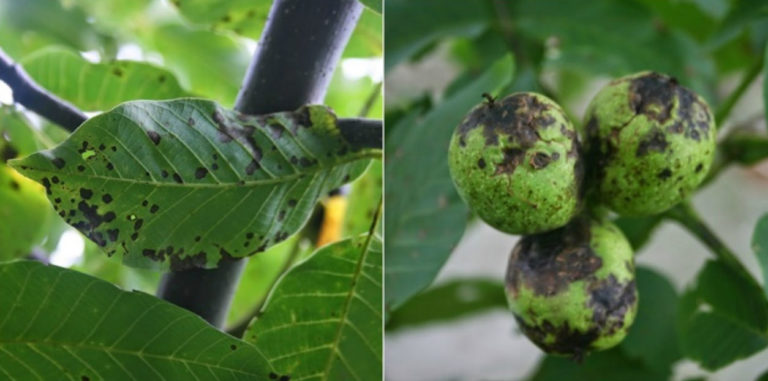
\includegraphics[width=10.67in]{Figures/walnutblight} 

}

\caption{Walnut blight symptoms. Credit: James E. Adaskaveg and Helga Förster}\label{fig:walnutblight}
\end{figure}

\chapter{Introduction}\label{intro}

The objective of this research is to characterize the population structure and prevalence of copper resistance of the walnut blight pathogen, \emph{Xanthomonas arboricola} pv. \emph{juglandis} ( \emph{Xaj} ) collected in central and Northern California between the years of 1994 to 2019. Additionally, we are interested in elucidating the type III secretion system effector (T3E) diversity and assessing where the Californian \emph{Xaj} population fits in a global context. We also sequenced 20 strains of \emph{Xanthomonas arboricola} pv. \emph{pruni} ( \emph{Xap} ), the causal agent of bacterial spot of almond, and included those in some of the analyses.

\section{Hypotheses}\label{hypotheses}

\begin{itemize}
\tightlist
\item
  Genes associated with and/or responsible for copper resistance are prevalent in the CA \emph{Xanthomonas arboricola} pv. \emph{juglandis} population and correlate
  with the respective copper-sensitivity phenotype \emph{in vitro}.
\item
  \emph{Xaj} and \emph{Xap} exhibit variation in type III secretion system effector repertoires.
\item
  CA \emph{Xaj} strains form distinct genetic clusters when compared with other global strains.
\item
  The CA \emph{Xaj} population does not encode any plasmids.
\end{itemize}

\chapter{Methods}\label{methods}

\section{Read Processing}\label{read-processing}

Whole-genome sequencing from Novogene generated high-quality reads (Table \ref{tab:SeqRes}). Novogene provides reads that have been filtered based on the following criteria:

\begin{enumerate}
\def\labelenumi{(\arabic{enumi})}
\item
  Remove reads containing adapters.
\item
  Remove reads containing N \textgreater{} 10\% (N represents the base cannot be determined).
\item
  Remove reads containing low quality (Qscore\textless= 5) base which is over 50\% of the total base.
\end{enumerate}

However, I performed an additional filtering step using FastP v0.23.4 (\citet{chen2018}). The filters I'm applying are as follows:

\begin{Shaded}
\begin{Highlighting}[]
\ExtensionTok{{-}q}\NormalTok{ 30 }\ErrorTok{(}\ExtensionTok{the}\NormalTok{ quality value that a base is qualified}\KeywordTok{)}
\ExtensionTok{{-}{-}detect\_adapter\_for\_pe} \ErrorTok{(}\ExtensionTok{automatically}\NormalTok{ detect adapter sequence based on paired end reads, and remove them}\KeywordTok{)}
\end{Highlighting}
\end{Shaded}

Since we received \textasciitilde2x the amount of sequencing data than we were quoted for, I chose to filter the data for the highest quality reads (q \(\geq 30\)). I also opted to enable the auto-detection for adapter removal. Novogene removes most adapter sequences but \textless{} 1\% of the read sets contain adapter sequences so FastP \emph{should} detect and remove the remainders. Please refer to \hyperref[fastp-script]{FastP.sh} (\ref{fastp-script}) for the script.

\section{Genome Assembly and Annotation}\label{genome-assembly-and-annotation}

Prior to settling on the pipeline detailed below, I tested several other pipelines that are detailed in \texttt{XAJ\_XAP\_Project.v1.md}, \texttt{AS\_Progress\_Report\_090924.v3.pptx}, and \texttt{Assembly\_Pipeline\_102424.pptx}. Based on the findings from the pipeline tests, we settled on the following steps for \emph{de novo} genome assembly and annotation (\ref{fig:AssemblyPipeline}):

\begin{enumerate}
\def\labelenumi{\arabic{enumi}.}
\tightlist
\item
  \emph{De novo} assembly using Platanus\_B v1.3.2 (\citet{Kajitani2020}).
\item
  Generate assembly stats via QUAST v5.1.0rc1 (\citet{gurevich2013}).
\item
  Scaffold contigs using Ragout v2.3 (\citet{Kolmogorov2014}).

  \begin{itemize}
  \tightlist
  \item
    Xaj isolate IVIA 1317 (NCBI Accession: GCF\_023375035.1) (\citet{cuesta2022}) was used as the reference for the Xaj population.
  \item
    Xap isolate 15-088 (NCBI Accession: GCF\_008761555.1) was used as the reference for the Xap population.
  \end{itemize}
\item
  Polish scaffolds with Pilon (\citet{Walker2014}).
\item
  Assess completeness and contamination with CheckM (\citet{Parks2015}).
\item
  Annotate with NCBI PGAP (\citet{Tatusova2016}).

  \begin{itemize}
  \tightlist
  \item
    Since I already generated the Bioproject and Biosamples I was able to generate NCBI-submission ready annotations.
  \item
    These are currently being processed by NCBI. Two samples had an error and I'm in communication with NCBI on how to resolve these errors.
  \end{itemize}
\end{enumerate}

\begin{figure}

{\centering 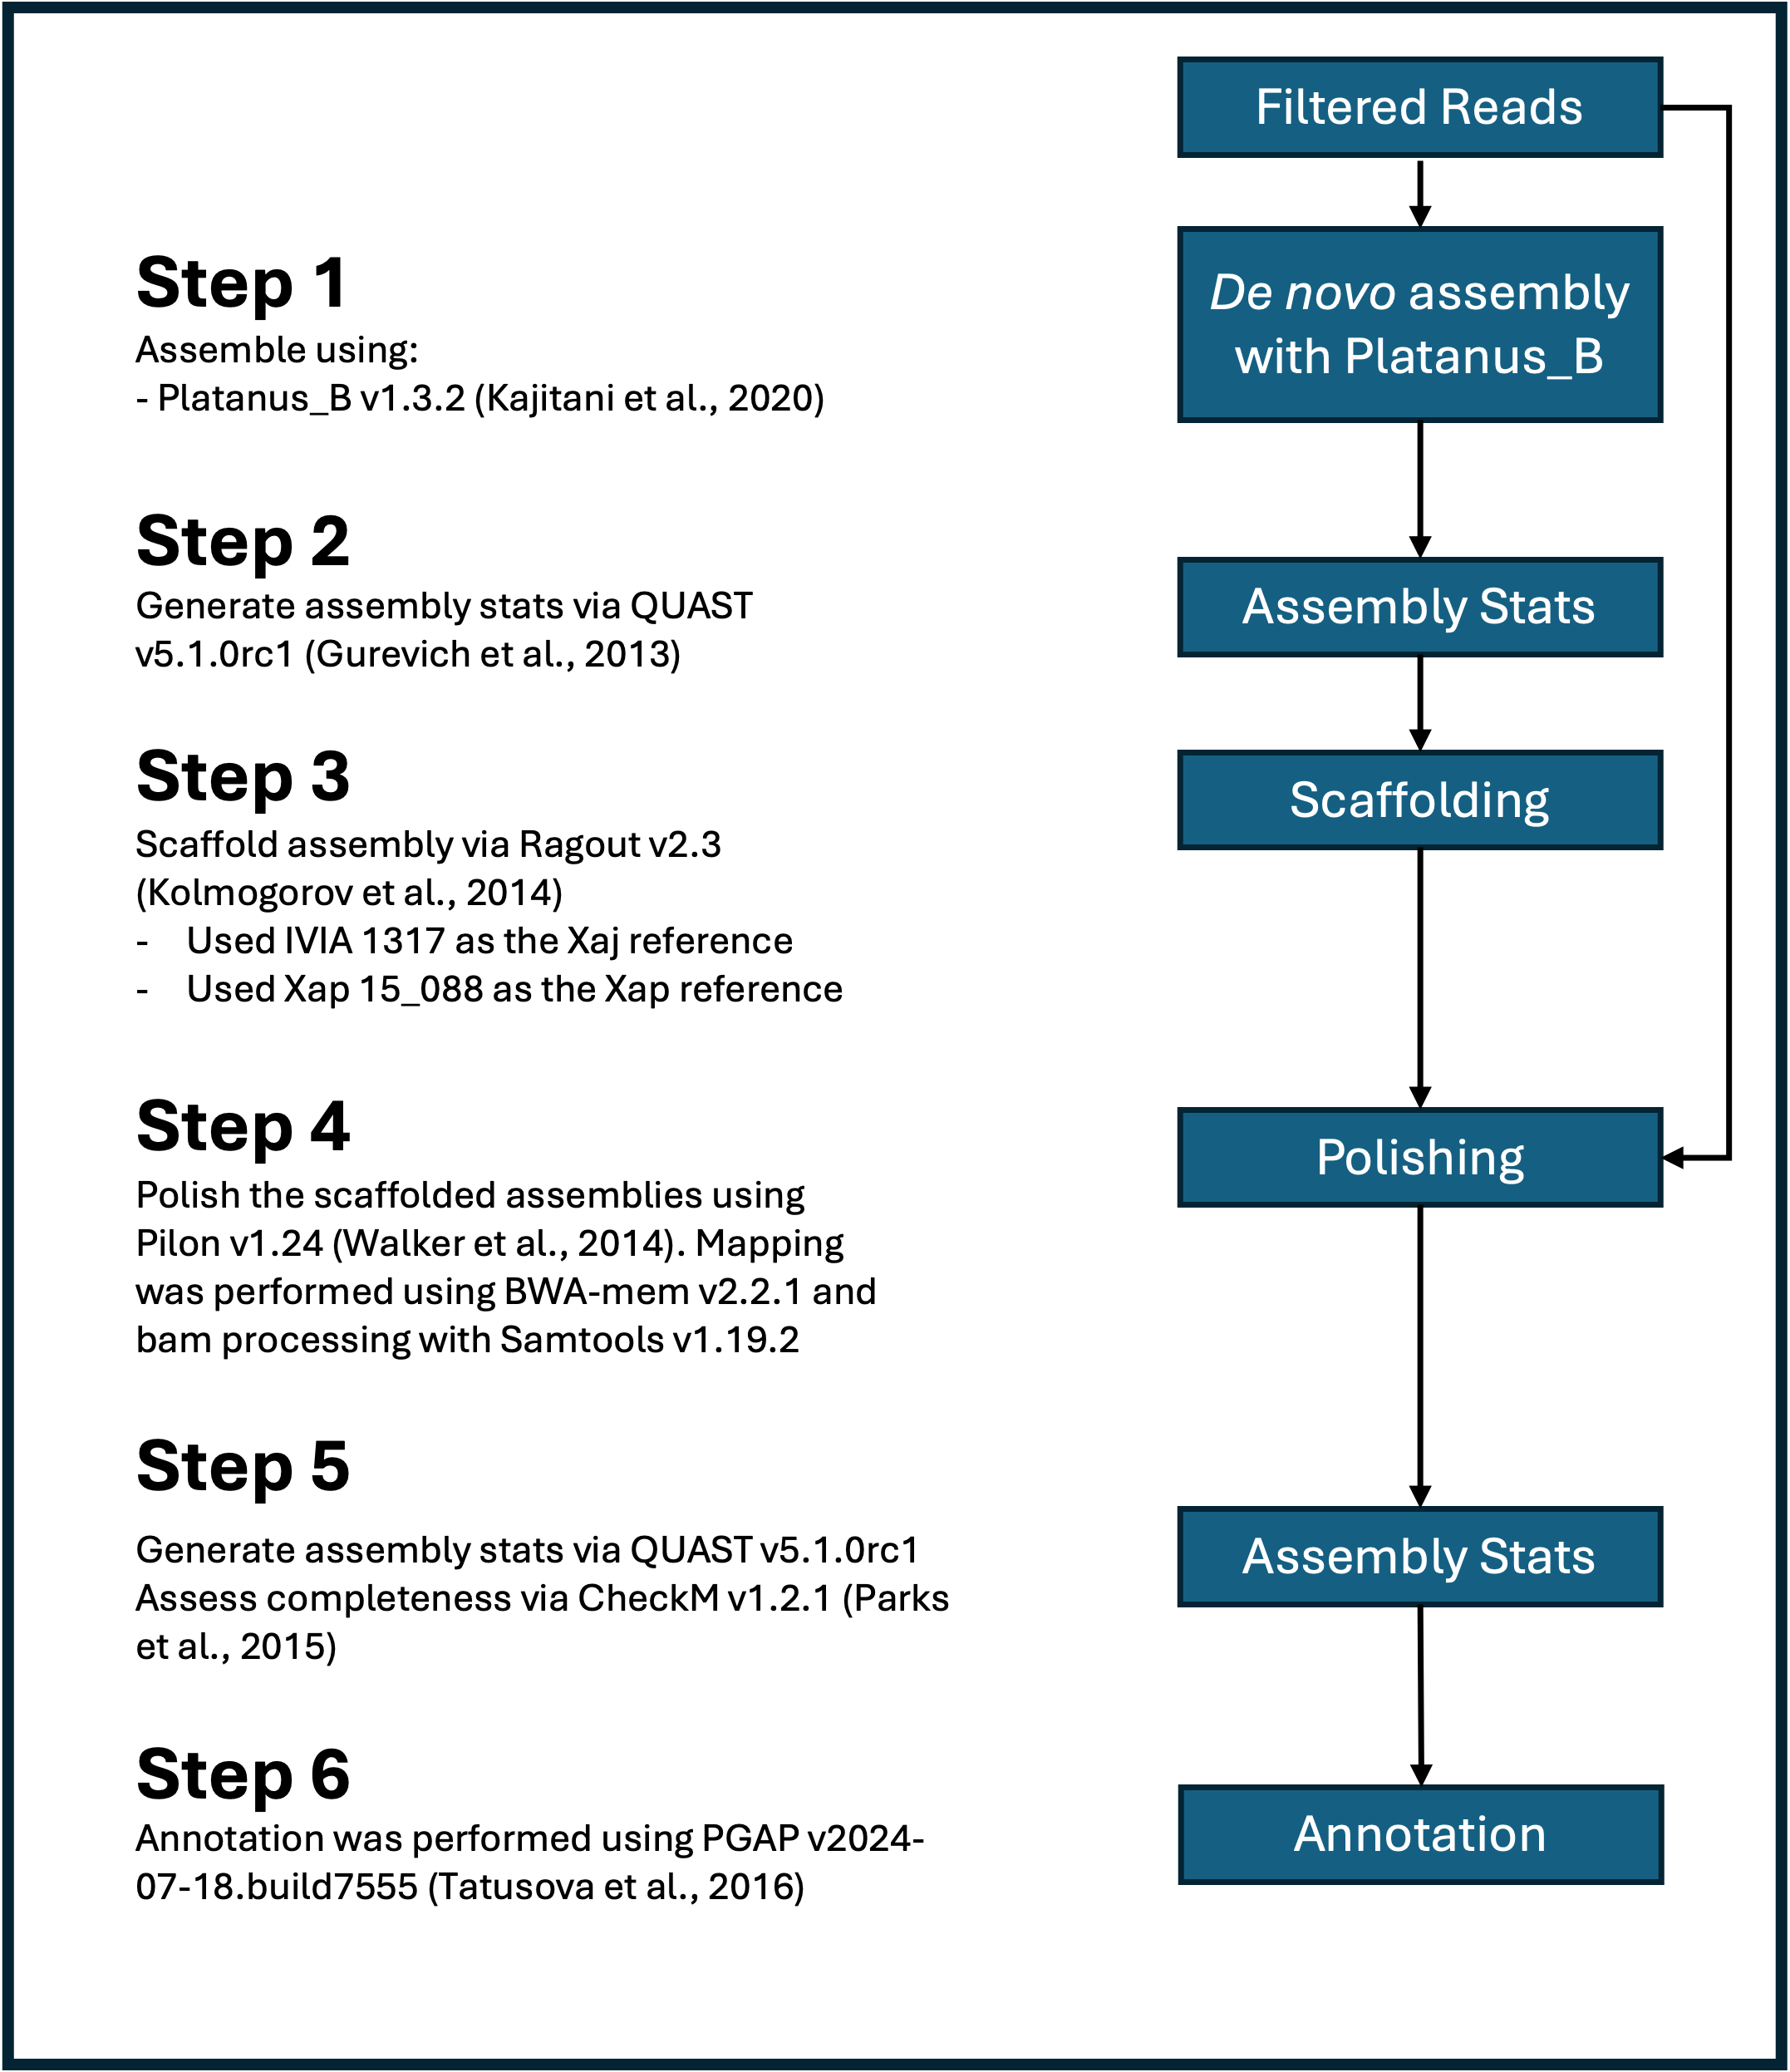
\includegraphics[width=0.8\linewidth,height=1\textheight]{Figures/Assembly_Pipeline} 

}

\caption{Xaj and Xap assembly pipeline}\label{fig:AssemblyPipeline}
\end{figure}

\subsection{Steps 1-2. Platanus\_B \& QUAST}\label{steps-1-2.-platanus_b-quast}

I generated \texttt{Assembly\_Workflow\_Platanus\_B.csv} and used it as my \texttt{\$SAMPFILE} variable for running Platanus\_B with the \hyperref[Assemble-script]{Step1.Assemble.sh} (\ref{Assemble-script}) script. It contains 5 columns that detail the sample ID, Strain, filtered Read1, filtered Read2, and organism. The \texttt{Assembly\_Workflow\_Platanus\_B.csv} file was converted to unix format using the \texttt{dos2unix} \texttt{Assembly\_Workflow\_Platanus\_B.csv} command on the cluster and afterwards the nano \texttt{Assembly\_Workflow\_Platanus\_B.csv} command was used to add one blank line at the end. \hyperref[Assemble-script]{Step1.Assemble.sh} (\ref{Assemble-script}) generated the de novo assemblies (contigs) and QUAST was used to generate assembly statistics.

I wrote a series of scripts to summarize the annotation and assembly results. These scripts are:

\hyperref[ANI-script]{Summarize\_ANI.sh} (\ref{ANI-script}), \hyperref[CheckM-script]{Summarize\_CheckM.sh} (\ref{CheckM-script}), and \hyperref[Genbank-script]{Summarize\_Genbank.py} (\ref{Genbank-script})

\subsection{Step 3. Scaffolding}\label{step-3.-scaffolding}

\texttt{Ragout\ v2.3} was used to scaffold the assemblies using \hyperref[Ragout-script]{Step2.Scaffold.sh} (\ref{Ragout-script}) . I used Xaj 417 and IVIA 1317 as reference strains for Xaj and 15-088 as the reference strain for Xap. As mentioned previously, we opted to proceed with the Ragout scaffolds using the IVIA 1317 reference since it gave better results (see \texttt{Assembly\_Pipeline\_102424.pptx}). QUAST was also used to generate statistics for comparisons.

Ragout uses \texttt{.rcp} files as inputs to set specific variables. I generated two template \texttt{.rcp} files for Xaj (\texttt{XAJ\_Template.rcp}) and Xap (\texttt{XAP\_Template.rcp}), respectively. These template files served as an input for \texttt{.rcp} file generation for each strain. \texttt{XAJ\_Strains.RCP.csv} and \texttt{XAP\_Strains.RCP.csv} served as input files for generating the \texttt{.rcp} files using \hyperref[RCP-script]{Generate\_RCP.sh} (\ref{RCP-script}).

\subsection{Step 4. Polishing with Pilon}\label{step-4.-polishing-with-pilon}

Based on the the previous findings (see \texttt{Assembly\_Pipeline\_102424.pptx}), Pilon increased assembly quality. \texttt{Pilon\ v1.24} using default settings were applied to the Ragout assemblies using \hyperref[Polish-script]{Step3.Polish.sh} (\ref{Polish-script}). I used \texttt{BWA-mem2\ v2.2.1} (\citet{Vasimuddin2019}), and \texttt{samtools\ v1.19.2} (\citet{Li2009}) prior to Pilon. These Pilon polished assemblies were used for the PGAP annotations. The Pilon-polished assemblies were then subjected to CheckM (\citet{Parks2015}) using the taxonomy option with \emph{Xanthomonas} as the reference genus to assess completeness and contamination (see \hyperref[CheckM2-script]{Step3.CheckM.sh} (\ref{CheckM2-script})).

\subsection{Step 5. Annotation}\label{step-5.-annotation}

I downloaded \texttt{PGAP\ v2024-07-18.build7555} on my local computer because I was running into issues trying to install it on the cluster. Since these assemblies and annotations will be submitted to NCBI, I needed to generate \texttt{\$STRAIN.generic.yaml} and \texttt{\$STRAIN.submol.yaml} as inputs for PGAP to ensure that all metadata is correctly assigned. I wrote \hyperref[GenYAML-script]{Generate\_Generic\_YAML.sh} (\ref{GenYAML-script}) and \hyperref[SubmolYAML-script]{Generate\_Submol\_YAML.sh} (\ref{SubmolYAML-script}) to efficiently generate the .yaml files. The metadata was stored in \texttt{Reference\_Data\_For\_YAML.txt} and each of the .yaml scripts used that file to generate the respective .yaml files. Next I wrote \hyperref[PGAP-script]{PGAP.sh} (\ref{PGAP-script}), the core PGAP command, to generate the annotations and I called that script using \hyperref[Annotate-script]{Step4.Annotate.sh} (\ref{Annotate-script}) because I was running this locally.

\subsection{NCBI Submission}\label{ncbi-submission}

Before we publish the manuscript we must submit our data (raw Illumina reads \& annotated assemblies) to NCBI. I submitted all the raw reads from Novogene to the SRA under the BioProject PRJNA1151720 (\ref{tab:SRA}). The SRA submission has already been processed and will be released upon publication. The genomes are currently being processed as of January 17,2025.

Unfortunately, XAJ2128 and XAJ934 had one error each that I must address before submission. The error is the same for both: \texttt{{[}SEQ\_FEAT.FeatureBeginsOrEndsInGap{]}\ Feature\ begins\ or\ ends\ in\ gap} and only occurs for one gene (transposase) in each strain, respectively. Specifically, the beginning of the genes start with an `N', but the respective protein started with an `M'. According to NCBI, the fix is to either remove the gene entirely or label the gene as `partial'. Since I've already performed genomic analyses (phylogeny, pangenome, etc.) I do not want to remove the gene. I emailed NCBI on January 21, 2025 to ask for assistance to make these changes to indicate that the transposase is indicated as `partial'. I'm confident that they will be able to help me make these changes. This is likely due to me using the \texttt{-\/-ignore-all-errors} argument in \hyperref[PGAP-script]{PGAP.sh} (\ref{PGAP-script}). I had to use that argument in order to make the program run.. otherwise the annotations would fail. It's fine as the other annotations are processing just fine.

Here are the BioProject details (please note that this information can be modified if needed, as I wrote these as placeholders):

\textbf{BioProject Accession:}

\begin{itemize}
\tightlist
\item
  PRJNA1151720
\end{itemize}

\textbf{Title:}

\begin{itemize}
\tightlist
\item
  Population genomics of \emph{Xanthomonas arboricola} pv. \emph{juglandis} and \emph{X. arboricola} pv. \emph{pruni} from California
\end{itemize}

\textbf{Description:}

\begin{itemize}
\tightlist
\item
  \emph{Xanthomonas arboricola} pv. \emph{juglandis} ( \emph{Xaj} ) and \emph{X. arboricola} pv. \emph{pruni} ( \emph{Xap} ) are the causal agents of walnut blight and bacterial spot of almond, respectively. California is the global leader in almond production and the top producer of walnuts in the United States, but both crops face challenges from \emph{Xaj} and \emph{Xap}, respectively. Moreover, the persistent use of copper-based bactericides has led to copper-resistant strains of \emph{Xaj} and \emph{Xap}. In this study, we sequenced and assembled the genomes of 120 \emph{Xaj} and 20 \emph{Xap} strains isolated from walnut and almond in Central and Northern California, respectively, to determine their population structure, detect copper resistance within the populations, and characterize their type III secretion system effector repertoires.
\end{itemize}

\begin{longtable}[]{@{}ccccc@{}}
\caption{\label{tab:SRA} List of all Xaj and Xap strains with SRA information.}\tabularnewline
\toprule\noalign{}
\textbf{Strain} & \textbf{BioSample} & \textbf{BioProject} & \textbf{Study} & \textbf{SRA Accession} \\
\midrule\noalign{}
\endfirsthead
\toprule\noalign{}
\textbf{Strain} & \textbf{BioSample} & \textbf{BioProject} & \textbf{Study} & \textbf{SRA Accession} \\
\midrule\noalign{}
\endhead
\bottomrule\noalign{}
\endlastfoot
XAJ1028 & SAMN43323323 & PRJNA1151720 & SRP528351 & SRR30358100 \\
XAJ1046 & SAMN43323324 & PRJNA1151720 & SRP528351 & SRR30358099 \\
XAJ1048 & SAMN43323325 & PRJNA1151720 & SRP528351 & SRR30358014 \\
XAJ1049 & SAMN43323326 & PRJNA1151720 & SRP528351 & SRR30358003 \\
XAJ1054 & SAMN43323327 & PRJNA1151720 & SRP528351 & SRR30357970 \\
XAJ1082 & SAMN43323328 & PRJNA1151720 & SRP528351 & SRR30358043 \\
XAJ1086 & SAMN43323329 & PRJNA1151720 & SRP528351 & SRR30358035 \\
XAJ1148 & SAMN43323330 & PRJNA1151720 & SRP528351 & SRR30358000 \\
XAJ1149 & SAMN43323331 & PRJNA1151720 & SRP528351 & SRR30357988 \\
XAJ1197 & SAMN43323332 & PRJNA1151720 & SRP528351 & SRR30358075 \\
XAJ1213 & SAMN43323333 & PRJNA1151720 & SRP528351 & SRR30358098 \\
XAJ1239 & SAMN43323334 & PRJNA1151720 & SRP528351 & SRR30358087 \\
XAJ1246 & SAMN43323335 & PRJNA1151720 & SRP528351 & SRR30358063 \\
XAJ1250 & SAMN43323336 & PRJNA1151720 & SRP528351 & SRR30358052 \\
XAJ1395 & SAMN43323337 & PRJNA1151720 & SRP528351 & SRR30358019 \\
XAJ1399 & SAMN43323338 & PRJNA1151720 & SRP528351 & SRR30358018 \\
XAJ145 & SAMN43323339 & PRJNA1151720 & SRP528351 & SRR30358021 \\
XAJ1498 & SAMN43323340 & PRJNA1151720 & SRP528351 & SRR30358017 \\
XAJ1535 & SAMN43323341 & PRJNA1151720 & SRP528351 & SRR30358016 \\
XAJ1537 & SAMN43323342 & PRJNA1151720 & SRP528351 & SRR30358015 \\
XAJ1539 & SAMN43323343 & PRJNA1151720 & SRP528351 & SRR30358013 \\
XAJ1551 & SAMN43323344 & PRJNA1151720 & SRP528351 & SRR30358012 \\
XAJ1554 & SAMN43323345 & PRJNA1151720 & SRP528351 & SRR30358011 \\
XAJ1556 & SAMN43323346 & PRJNA1151720 & SRP528351 & SRR30358010 \\
XAJ1557 & SAMN43323347 & PRJNA1151720 & SRP528351 & SRR30358009 \\
XAJ1558 & SAMN43323348 & PRJNA1151720 & SRP528351 & SRR30358008 \\
XAJ1595 & SAMN43323349 & PRJNA1151720 & SRP528351 & SRR30358007 \\
XAJ1606 & SAMN43323350 & PRJNA1151720 & SRP528351 & SRR30358006 \\
XAJ1613 & SAMN43323351 & PRJNA1151720 & SRP528351 & SRR30358005 \\
XAJ1614 & SAMN43323352 & PRJNA1151720 & SRP528351 & SRR30358004 \\
XAJ1615 & SAMN43323353 & PRJNA1151720 & SRP528351 & SRR30357980 \\
XAJ1616 & SAMN43323354 & PRJNA1151720 & SRP528351 & SRR30357979 \\
XAJ1617 & SAMN43323355 & PRJNA1151720 & SRP528351 & SRR30357978 \\
XAJ1626 & SAMN43323356 & PRJNA1151720 & SRP528351 & SRR30357977 \\
XAJ163 & SAMN43323357 & PRJNA1151720 & SRP528351 & SRR30357976 \\
XAJ165 & SAMN43323358 & PRJNA1151720 & SRP528351 & SRR30357975 \\
XAJ169 & SAMN43323359 & PRJNA1151720 & SRP528351 & SRR30357974 \\
XAJ1710 & SAMN43323360 & PRJNA1151720 & SRP528351 & SRR30357973 \\
XAJ1711 & SAMN43323361 & PRJNA1151720 & SRP528351 & SRR30357972 \\
XAJ1808 & SAMN43323362 & PRJNA1151720 & SRP528351 & SRR30357971 \\
XAJ181 & SAMN43323363 & PRJNA1151720 & SRP528351 & SRR30357969 \\
XAJ1822 & SAMN43323364 & PRJNA1151720 & SRP528351 & SRR30357968 \\
XAJ1824 & SAMN43323365 & PRJNA1151720 & SRP528351 & SRR30357967 \\
XAJ2122 & SAMN43323366 & PRJNA1151720 & SRP528351 & SRR30357966 \\
XAJ2124 & SAMN43323367 & PRJNA1151720 & SRP528351 & SRR30357965 \\
XAJ2125 & SAMN43323368 & PRJNA1151720 & SRP528351 & SRR30357964 \\
XAJ2128 & SAMN43323369 & PRJNA1151720 & SRP528351 & SRR30357963 \\
XAJ2129 & SAMN43323370 & PRJNA1151720 & SRP528351 & SRR30357962 \\
XAJ2131 & SAMN43323371 & PRJNA1151720 & SRP528351 & SRR30357961 \\
XAJ2165 & SAMN43323372 & PRJNA1151720 & SRP528351 & SRR30358044 \\
XAJ2167 & SAMN43323373 & PRJNA1151720 & SRP528351 & SRR30358042 \\
XAJ2169 & SAMN43323374 & PRJNA1151720 & SRP528351 & SRR30358041 \\
XAJ2170 & SAMN43323375 & PRJNA1151720 & SRP528351 & SRR30358040 \\
XAJ2178 & SAMN43323376 & PRJNA1151720 & SRP528351 & SRR30358039 \\
XAJ2180 & SAMN43323377 & PRJNA1151720 & SRP528351 & SRR30358038 \\
XAJ283A & SAMN43323378 & PRJNA1151720 & SRP528351 & SRR30358037 \\
XAJ283B & SAMN43323379 & PRJNA1151720 & SRP528351 & SRR30358036 \\
XAJ30 & SAMN43323380 & PRJNA1151720 & SRP528351 & SRR30358034 \\
XAJ31 & SAMN43323381 & PRJNA1151720 & SRP528351 & SRR30358033 \\
XAJ32 & SAMN43323382 & PRJNA1151720 & SRP528351 & SRR30358032 \\
XAJ321 & SAMN43323383 & PRJNA1151720 & SRP528351 & SRR30358031 \\
XAJ322 & SAMN43323384 & PRJNA1151720 & SRP528351 & SRR30358030 \\
XAJ33 & SAMN43323385 & PRJNA1151720 & SRP528351 & SRR30358029 \\
XAJ330 & SAMN43323386 & PRJNA1151720 & SRP528351 & SRR30358028 \\
XAJ333 & SAMN43323387 & PRJNA1151720 & SRP528351 & SRR30358026 \\
XAJ338 & SAMN43323388 & PRJNA1151720 & SRP528351 & SRR30358025 \\
XAJ34 & SAMN43323389 & PRJNA1151720 & SRP528351 & SRR30358024 \\
XAJ340 & SAMN43323390 & PRJNA1151720 & SRP528351 & SRR30358027 \\
XAJ341 & SAMN43323391 & PRJNA1151720 & SRP528351 & SRR30358002 \\
XAJ344 & SAMN43323392 & PRJNA1151720 & SRP528351 & SRR30358001 \\
XAJ345 & SAMN43323393 & PRJNA1151720 & SRP528351 & SRR30357999 \\
XAJ347 & SAMN43323394 & PRJNA1151720 & SRP528351 & SRR30357997 \\
XAJ349 & SAMN43323395 & PRJNA1151720 & SRP528351 & SRR30357996 \\
XAJ35 & SAMN43323396 & PRJNA1151720 & SRP528351 & SRR30357995 \\
XAJ355 & SAMN43323397 & PRJNA1151720 & SRP528351 & SRR30357998 \\
XAJ36 & SAMN43323398 & PRJNA1151720 & SRP528351 & SRR30357994 \\
XAJ372 & SAMN43323399 & PRJNA1151720 & SRP528351 & SRR30357993 \\
XAJ38 & SAMN43323400 & PRJNA1151720 & SRP528351 & SRR30357992 \\
XAJ390 & SAMN43323401 & PRJNA1151720 & SRP528351 & SRR30357991 \\
XAJ402 & SAMN43323402 & PRJNA1151720 & SRP528351 & SRR30357989 \\
XAJ426 & SAMN43323403 & PRJNA1151720 & SRP528351 & SRR30357987 \\
XAJ427 & SAMN43323404 & PRJNA1151720 & SRP528351 & SRR30357990 \\
XAJ428 & SAMN43323405 & PRJNA1151720 & SRP528351 & SRR30357986 \\
XAJ432 & SAMN43323406 & PRJNA1151720 & SRP528351 & SRR30357985 \\
XAJ435 & SAMN43323407 & PRJNA1151720 & SRP528351 & SRR30357984 \\
XAJ438 & SAMN43323408 & PRJNA1151720 & SRP528351 & SRR30357983 \\
XAJ439 & SAMN43323409 & PRJNA1151720 & SRP528351 & SRR30357981 \\
XAJ456 & SAMN43323410 & PRJNA1151720 & SRP528351 & SRR30358077 \\
XAJ458 & SAMN43323411 & PRJNA1151720 & SRP528351 & SRR30358076 \\
XAJ462 & SAMN43323412 & PRJNA1151720 & SRP528351 & SRR30357982 \\
XAJ464 & SAMN43323413 & PRJNA1151720 & SRP528351 & SRR30358074 \\
XAJ465 & SAMN43323414 & PRJNA1151720 & SRP528351 & SRR30358073 \\
XAJ466 & SAMN43323415 & PRJNA1151720 & SRP528351 & SRR30358072 \\
XAJ467 & SAMN43323416 & PRJNA1151720 & SRP528351 & SRR30358070 \\
XAJ469 & SAMN43323417 & PRJNA1151720 & SRP528351 & SRR30358069 \\
XAJ470 & SAMN43323418 & PRJNA1151720 & SRP528351 & SRR30358068 \\
XAJ473 & SAMN43323419 & PRJNA1151720 & SRP528351 & SRR30358071 \\
XAJ476 & SAMN43323420 & PRJNA1151720 & SRP528351 & SRR30358067 \\
XAJ477 & SAMN43323421 & PRJNA1151720 & SRP528351 & SRR30358066 \\
XAJ669 & SAMN43323422 & PRJNA1151720 & SRP528351 & SRR30358064 \\
XAJ670 & SAMN43323423 & PRJNA1151720 & SRP528351 & SRR30358097 \\
XAJ671 & SAMN43323424 & PRJNA1151720 & SRP528351 & SRR30358096 \\
XAJ672 & SAMN43323425 & PRJNA1151720 & SRP528351 & SRR30358095 \\
XAJ673 & SAMN43323426 & PRJNA1151720 & SRP528351 & SRR30358094 \\
XAJ674 & SAMN43323427 & PRJNA1151720 & SRP528351 & SRR30358093 \\
XAJ675 & SAMN43323428 & PRJNA1151720 & SRP528351 & SRR30358092 \\
XAJ729 & SAMN43323429 & PRJNA1151720 & SRP528351 & SRR30358090 \\
XAJ730 & SAMN43323430 & PRJNA1151720 & SRP528351 & SRR30358089 \\
XAJ731 & SAMN43323431 & PRJNA1151720 & SRP528351 & SRR30358088 \\
XAJ929 & SAMN43323432 & PRJNA1151720 & SRP528351 & SRR30358091 \\
XAJ930 & SAMN43323433 & PRJNA1151720 & SRP528351 & SRR30358086 \\
XAJ934 & SAMN43323434 & PRJNA1151720 & SRP528351 & SRR30358085 \\
XAJ935 & SAMN43323435 & PRJNA1151720 & SRP528351 & SRR30358084 \\
XAJ936 & SAMN43323436 & PRJNA1151720 & SRP528351 & SRR30358082 \\
XAJ939 & SAMN43323437 & PRJNA1151720 & SRP528351 & SRR30358081 \\
XAJ940 & SAMN43323438 & PRJNA1151720 & SRP528351 & SRR30358080 \\
XAJ968 & SAMN43323439 & PRJNA1151720 & SRP528351 & SRR30358083 \\
XAJ969 & SAMN43323440 & PRJNA1151720 & SRP528351 & SRR30358079 \\
XAJ973 & SAMN43323441 & PRJNA1151720 & SRP528351 & SRR30358078 \\
XAJ984 & SAMN43323442 & PRJNA1151720 & SRP528351 & SRR30358065 \\
XAP1007 & SAMN43323443 & PRJNA1151720 & SRP528351 & SRR30358062 \\
XAP1010 & SAMN43323444 & PRJNA1151720 & SRP528351 & SRR30358061 \\
XAP1159 & SAMN43323445 & PRJNA1151720 & SRP528351 & SRR30358060 \\
XAP1265 & SAMN43323446 & PRJNA1151720 & SRP528351 & SRR30358059 \\
XAP1657 & SAMN43323447 & PRJNA1151720 & SRP528351 & SRR30358058 \\
XAP1741 & SAMN43323448 & PRJNA1151720 & SRP528351 & SRR30358057 \\
XAP2004 & SAMN43323449 & PRJNA1151720 & SRP528351 & SRR30358056 \\
XAP2016 & SAMN43323450 & PRJNA1151720 & SRP528351 & SRR30358055 \\
XAP2023 & SAMN43323451 & PRJNA1151720 & SRP528351 & SRR30358054 \\
XAP2029 & SAMN43323452 & PRJNA1151720 & SRP528351 & SRR30358053 \\
XAP2036 & SAMN43323453 & PRJNA1151720 & SRP528351 & SRR30358051 \\
XAP2039 & SAMN43323454 & PRJNA1151720 & SRP528351 & SRR30358050 \\
XAP2106 & SAMN43323455 & PRJNA1151720 & SRP528351 & SRR30358049 \\
XAP2113 & SAMN43323456 & PRJNA1151720 & SRP528351 & SRR30358048 \\
XAP2150 & SAMN43323457 & PRJNA1151720 & SRP528351 & SRR30358047 \\
XAP664 & SAMN43323458 & PRJNA1151720 & SRP528351 & SRR30358046 \\
XAP667 & SAMN43323459 & PRJNA1151720 & SRP528351 & SRR30358045 \\
XAP880 & SAMN43323460 & PRJNA1151720 & SRP528351 & SRR30358023 \\
XAP883 & SAMN43323461 & PRJNA1151720 & SRP528351 & SRR30358022 \\
XAP948 & SAMN43323462 & PRJNA1151720 & SRP528351 & SRR30358020 \\
\end{longtable}

\subsection{\texorpdfstring{\emph{Xaj}, \emph{Xap}, and \emph{Xhg} RefSeq Genomic Resources}{Xaj, Xap, and Xhg RefSeq Genomic Resources}}\label{xaj-xap-and-xhg-refseq-genomic-resources}

I downloaded several RefSeq accessions for various \emph{Xaj}, \emph{Xap} and \emph{X. hortorum} pv. \emph{gardneri} ( \emph{Xhg} ) for my phylogenetic analyses (\ref{tab:RefSeq}).

\begin{longtable}[]{@{}
  >{\centering\arraybackslash}p{(\columnwidth - 20\tabcolsep) * \real{0.0909}}
  >{\centering\arraybackslash}p{(\columnwidth - 20\tabcolsep) * \real{0.0909}}
  >{\centering\arraybackslash}p{(\columnwidth - 20\tabcolsep) * \real{0.0909}}
  >{\centering\arraybackslash}p{(\columnwidth - 20\tabcolsep) * \real{0.0909}}
  >{\centering\arraybackslash}p{(\columnwidth - 20\tabcolsep) * \real{0.0909}}
  >{\centering\arraybackslash}p{(\columnwidth - 20\tabcolsep) * \real{0.0909}}
  >{\centering\arraybackslash}p{(\columnwidth - 20\tabcolsep) * \real{0.0909}}
  >{\centering\arraybackslash}p{(\columnwidth - 20\tabcolsep) * \real{0.0909}}
  >{\centering\arraybackslash}p{(\columnwidth - 20\tabcolsep) * \real{0.0909}}
  >{\centering\arraybackslash}p{(\columnwidth - 20\tabcolsep) * \real{0.0909}}
  >{\centering\arraybackslash}p{(\columnwidth - 20\tabcolsep) * \real{0.0909}}@{}}
\caption{\label{tab:RefSeq} NCBI RefSeq accessions for \emph{Xap} (n=22), \emph{Xaj} (n=26) and \emph{Xhg} (n=1) genome(s) used in analyses. The sample collection date, host and location information for NCPPB 1447 was found in Table 1. (\citet{Scortichini2001}).}\tabularnewline
\toprule\noalign{}
\begin{minipage}[b]{\linewidth}\centering
\textbf{Accession}
\end{minipage} & \begin{minipage}[b]{\linewidth}\centering
\textbf{BioProject Accession}
\end{minipage} & \begin{minipage}[b]{\linewidth}\centering
\textbf{Protein Coding Genes}
\end{minipage} & \begin{minipage}[b]{\linewidth}\centering
\textbf{Gene count total}
\end{minipage} & \begin{minipage}[b]{\linewidth}\centering
\textbf{Assembly level}
\end{minipage} & \begin{minipage}[b]{\linewidth}\centering
\textbf{Organism}
\end{minipage} & \begin{minipage}[b]{\linewidth}\centering
\textbf{Number of Component Sequences}
\end{minipage} & \begin{minipage}[b]{\linewidth}\centering
\textbf{Strain}
\end{minipage} & \begin{minipage}[b]{\linewidth}\centering
\textbf{Collection Date}
\end{minipage} & \begin{minipage}[b]{\linewidth}\centering
\textbf{Host}
\end{minipage} & \begin{minipage}[b]{\linewidth}\centering
\textbf{Location}
\end{minipage} \\
\midrule\noalign{}
\endfirsthead
\toprule\noalign{}
\begin{minipage}[b]{\linewidth}\centering
\textbf{Accession}
\end{minipage} & \begin{minipage}[b]{\linewidth}\centering
\textbf{BioProject Accession}
\end{minipage} & \begin{minipage}[b]{\linewidth}\centering
\textbf{Protein Coding Genes}
\end{minipage} & \begin{minipage}[b]{\linewidth}\centering
\textbf{Gene count total}
\end{minipage} & \begin{minipage}[b]{\linewidth}\centering
\textbf{Assembly level}
\end{minipage} & \begin{minipage}[b]{\linewidth}\centering
\textbf{Organism}
\end{minipage} & \begin{minipage}[b]{\linewidth}\centering
\textbf{Number of Component Sequences}
\end{minipage} & \begin{minipage}[b]{\linewidth}\centering
\textbf{Strain}
\end{minipage} & \begin{minipage}[b]{\linewidth}\centering
\textbf{Collection Date}
\end{minipage} & \begin{minipage}[b]{\linewidth}\centering
\textbf{Host}
\end{minipage} & \begin{minipage}[b]{\linewidth}\centering
\textbf{Location}
\end{minipage} \\
\midrule\noalign{}
\endhead
\bottomrule\noalign{}
\endlastfoot
GCF\_000306055.1 & PRJNA84273 & 4155 & 4517 & Contig & Xaj & 371 & NCPPB 1447 & 1963 & Juglans & Romnia \\
GCF\_001013475.1 & PRJNA275685 & 4165 & 4387 & Scaffold & Xaj & 8 & CFBP 2528 & 1956 & Juglans regia & New Zealand \\
GCF\_001013495.1 & PRJNA275691 & 4238 & 4477 & Scaffold & Xaj & 14 & CFBP 7179 & 2002 & Juglans regia & France:Lot-et-Garonne \\
GCF\_001237985.1 & PRJNA291479 & 4216 & 4454 & Chromosome & Xaj & 1 & Xaj 417 & 2012 & Juglans regia & USA \\
GCF\_001643295.1 & PRJNA310300 & 4148 & 4385 & Contig & Xaj & 161 & J303 & 2011 & Juglans regia & Chile: Concepcion \\
GCF\_002879695.1 & PRJNA428855 & 4191 & 4415 & Contig & Xaj & 8 & DW3F3 & 2015 & walnut (Juglans regia L. cv. Qingxiang). & China: Hubei Province, Danjiangkou City \\
GCF\_002940235.1 & PRJNA339511 & 4059 & 4279 & Contig & Xaj & 91 & CFBP 8253 & 2002 & Juglans regia cv. Franquette & France: Isere, Saint Hilaire Le Rosier \\
GCF\_023375035.1 & PRJNA736723 & 4269 & 4502 & Complete Genome & Xaj & 1 & IVIA 1317 & 1993 & Juglans regia & Spain \\
GCF\_023375055.1 & PRJNA736725 & 4275 & 4508 & Complete Genome & Xaj & 1 & IVIA 2499 & 2001 & Juglans regia & Spain \\
GCF\_030388855.1 & PRJNA982436 & 4012 & 4235 & Contig & Xaj & 78 & OS5 & 2020 & Juglans & Serbia:Sirig \\
GCF\_030388865.1 & PRJNA982436 & 4245 & 4471 & Contig & Xaj & 80 & OVM2 & 2020 & Juglans & Serbia:Milicinica \\
GCF\_030388905.1 & PRJNA982436 & 4242 & 4466 & Contig & Xaj & 81 & OVM3 & 2020 & Juglans & Serbia:Milicinica \\
GCF\_030388925.1 & PRJNA982436 & 4025 & 4248 & Contig & Xaj & 81 & OS2 & 2020 & Juglans & Serbia:Sirig \\
GCF\_030388945.1 & PRJNA982436 & 4247 & 4473 & Contig & Xaj & 79 & OVM1 & 2020 & Juglans & Serbia:Milicinica \\
GCF\_030388965.1 & PRJNA982436 & 4244 & 4465 & Contig & Xaj & 76 & OC4 & 2020 & Juglans & Serbia:Crvenka \\
GCF\_030388985.1 & PRJNA982436 & 4250 & 4471 & Contig & Xaj & 75 & OC3 & 2020 & Juglans & Serbia:Crvenka \\
GCF\_030388995.1 & PRJNA982436 & 4245 & 4468 & Contig & Xaj & 75 & OC1 & 2020 & Juglans & Serbia:Crvenka \\
GCF\_030389015.1 & PRJNA982436 & 4249 & 4471 & Contig & Xaj & 75 & OC2 & 2020 & Juglans & Serbia:Crvenka \\
GCF\_030389445.1 & PRJNA982436 & 4107 & 4335 & Contig & Xaj & 75 & XjL1 & 2019 & Juglans & Serbia:Prokuplje \\
GCF\_030389555.1 & PRJNA982436 & 4096 & 4318 & Contig & Xaj & 82 & OS3 & 2020 & Juglans & Serbia:Sirig \\
GCF\_030389575.1 & PRJNA982436 & 4031 & 4252 & Contig & Xaj & 77 & OS4 & 2020 & Juglans & Serbia:Sirig \\
GCF\_040201855.1 & PRJNA991976 & 4204 & 4417 & Scaffold & Xaj & 68 & WHRI 5692A & 1996 & Juglans regia & United Kingdom \\
GCF\_900476315.1 & PRJEB27248 & 4260 & 4528 & Contig & Xaj & 56 & CPBF 1521 & 2014 & Juglans regia & Portugal \\
GCF\_903989475.2 & PRJEB39139 & 4258 & 4490 & Complete Genome & Xaj & 1 & CPBF 427 & 2016 & Juglans regia & Portugal \\
GCF\_905367715.1 & PRJEB43653 & 4170 & 4314 & Complete Genome & Xaj & 1 & CPBF 1494 & 2014 & Carya illinoinensis & Portugal \\
GCF\_905367745.1 & PRJEB43653 & 4249 & 4399 & Complete Genome & Xaj & 1 & CPBF 765 & 2016 & Carya illinoinensis & Portugal \\
GCF\_001741965.1 & PRJNA305230 & 4070 & 4353 & Scaffold & Xap & 77 & CFBP 3894 & 1953 & Prunus salicina & New Zealand: Auckland \\
GCF\_003984685.1 & PRJNA509257 & 4110 & 4411 & Contig & Xap & 57 & CITA 9 & 2008 & Prunus persica & Spain: Aragon \\
GCF\_003984725.1 & PRJNA509270 & 4113 & 4410 & Contig & Xap & 60 & CITA 99 & 2006 & Prunus dulcis & Spain: Alicante \\
GCF\_008761555.1 & PRJNA573813 & 4136 & 4424 & Complete Genome & Xap & 1 & 15-088 & 2015 & Prunus persica & South Korea \\
GCF\_020002335.2 & PRJNA762221 & 4151 & 4462 & Complete Genome & Xap & 3 & R1 & 2020 & Prunus persica & USA: South Carolina \\
GCF\_020012115.1 & PRJNA762222 & 4291 & 4604 & Contig & Xap & 190 & F1 & 2020 & Prunus persica & USA: South Carolina \\
GCF\_020012175.1 & PRJNA762223 & 4132 & 4425 & Contig & Xap & 174 & M1 & 2017 & Prunus persica & USA: South Carolina \\
GCF\_020043425.2 & PRJNA762226 & 4148 & 4463 & Complete Genome & Xap & 3 & T1 & 2017 & Prunus persica & USA: South Carolina \\
GCF\_021733585.2 & PRJNA796325 & 4144 & 4441 & Complete Genome & Xap & 2 & Xcp1 & 1992 & Prunus persica var. nucipersica & USA:North Carolina \\
GCF\_023375015.1 & PRJNA736578 & 4140 & 4426 & Complete Genome & Xap & 2 & IVIA 2626.1 & 2002 & Prunus salicina & Spain \\
GCF\_023375075.1 & PRJNA737276 & 4116 & 4410 & Complete Genome & Xap & 2 & CITA 33 & 2009 & Prunus dulcis & Spain \\
GCF\_030388845.1 & PRJNA982436 & 4083 & 4358 & Contig & Xap & 90 & Xp10 & 2019 & Prunus persica & Montenegro \\
GCF\_030389325.1 & PRJNA982436 & 4090 & 4369 & Contig & Xap & 76 & Xp720 & 2020 & Prunus armeniaca & Serbia:Besenovo \\
GCF\_030389345.1 & PRJNA982436 & 4093 & 4367 & Contig & Xap & 75 & Xp520 & 2020 & Prunus armeniaca & Serbia:Besenovo \\
GCF\_030389365.1 & PRJNA982436 & 4078 & 4351 & Contig & Xap & 78 & Xp419 & 2019 & Prunus persica & Serbia:Irig \\
GCF\_030389375.1 & PRJNA982436 & 4141 & 4423 & Contig & Xap & 79 & Xp619 & 2019 & Prunus persica & Serbia:Irig \\
GCF\_030389385.1 & PRJNA982436 & 4094 & 4369 & Contig & Xap & 77 & Xp320 & 2020 & Prunus armeniaca & Serbia:Besenovo \\
GCF\_030389435.1 & PRJNA982436 & 4091 & 4370 & Contig & Xap & 80 & Xp1 & 2019 & Prunus persica & Montenegro \\
GCF\_030389455.1 & PRJNA982436 & 4082 & 4358 & Contig & Xap & 87 & Xp4 & 2019 & Prunus persica & Montenegro \\
GCF\_030389485.1 & PRJNA982436 & 4055 & 4337 & Contig & Xap & 78 & Xp7 & 2019 & Prunus persica & Montenegro \\
GCF\_030389525.1 & PRJNA982436 & 4087 & 4363 & Contig & Xap & 79 & Xp219 & 2019 & Prunus persica & Serbia:Irig \\
GCF\_036541245.1 & PRJNA1061488 & 4089 & 4370 & Scaffold & Xap & 60 & PVCT 262.1 & 2020 & Prunus dulcis & Italy:Sicily \\
GCF\_001908755.1 & PRJNA344031 & 4437 & 4687 & Complete Genome & Xhg & 3 & JS749-3 & 1997 & Solanum lycopersicum & Réunion \\
\end{longtable}

\section{\texorpdfstring{\emph{In Vitro} Copper Sensistivity}{In Vitro Copper Sensistivity}}\label{in-vitro-copper-sensistivity}

I screened the 120 \emph{Xaj} and 20 \emph{Xap} strains for copper sensitivity using NA agar amended with copper sulfate (\(CuSO_4\)). We performed this in duplicates using the following concentrations: 0 (control), 1k, 5k, 7.5k, and 10k ppm. Strains were incubated at room temperature (22-25\(^\circ\)C) for 3 days before measuring.

\section{Pangenome Analyses}\label{pangenome-analyses}

\texttt{PPanGGOLiN\ v2.2.0} (\citet{Gautreau2020}) will be used to generate the pangenomes for this study. I will run several different combinations of samples that include the RefSeq genomes (\ref{tab:RefSeq}). I chose to use PPanGGOLiN because I found the output files to be very user-friendly and clearly defines regions of genomic plasticity (RGPs) (e.g.~Genomic Islands) and it's been widely cited (\textasciitilde180). The primary use of PPanGGOLiN in our study will be to generate a presence-absence matrix that will help with the identification of copper resistance-related genes, type 3 secretion system effectors, and identify RGPs associated with these respective genes.

Several runs of PPanGGOLiN were performed including:

\begin{enumerate}
\def\labelenumi{\arabic{enumi}.}
\tightlist
\item
  California \emph{Xaj} (n=120 and n=115)
\item
  California \emph{Xap} (n=20)
\item
  California \emph{Xaj} + 26 NCBI RefSeq \emph{Xaj} strians (n=146 and n=141)
\item
  California \emph{Xaj} + 24 NCBI RefSeq \emph{Xaj} strians (No pecan strains: CPBF 1494 and CPBF 765) (n=144 and n=139)
\item
  California \emph{Xap} + 22 NCBI RefSeq \emph{Xaj} strians (n=42)
\item
  California \emph{Xaj} + NCBI RefSeq \emph{Xaj} strians + California \emph{Xap} + NCBI RefSeq \emph{Xaj} strians (n=188 and n=183)
\item
  California \emph{Xaj} + NCBI RefSeq \emph{Xaj} strians + California \emph{Xap} + NCBI RefSeq \emph{Xaj} strians + NCBI RefSeq \emph{Xhg} (outgroup) (n=189 and n=184)
\item
  California \emph{Xaj} + California \emph{Xap} (n=140 and n=135)
\end{enumerate}

\textbf{NOTE}: The alternative values (e.g.~115, 141, etc.) are referring to the five `problematic strains' that were removed because the genomic data (e.g.~presence of copper resistance-related genes) did not align with the \emph{in vitro} copper sensitivity data (See Section \ref{CuSensitivity}).

Here are the respective directories for the analyses above (Not shown are the directories with \_115):

\begin{enumerate}
\def\labelenumi{\arabic{enumi}.}
\tightlist
\item
  CA\_XAJ
\item
  CA\_XAP
\item
  CA\_XAJ\_and\_NCBI26
\item
  CA\_XAJ\_and\_NCBI24
\item
  CA\_XAP\_and\_NCBI22
\item
  CA\_XAJ\_XAP\_and\_NCBI\_XAJ\_XAP
\item
  CA\_XAJ\_XAP\_and\_NCBI\_XAJ\_XAP\_and\_Outgroup
\end{enumerate}

\textbf{PPanGGOLiN Workflow}

\begin{enumerate}
\def\labelenumi{\arabic{enumi}.}
\tightlist
\item
  Run PPanGGOLiN using the \texttt{-all} mode to run all the pangenome analyses using \hyperref[Ppang-script]{PPanggolin.sh} (\ref{Ppang-script}).
\item
  Generate MSA of the `shell' genome for each run. (NEED TO RUN 11/25/24)
\end{enumerate}

PPanGGOLiN requires a \texttt{.tsv} file that contains two columns: strain and path to \texttt{.gbk} files. I created a \texttt{.tsv} named after the respective directories above but with the \texttt{\_Path.tsv} suffix. Each run had its own script, and both the script and .tsv files were in their respective directories, see \hyperref[PpangTSV-script]{PPanggolin\_TSV.sh} (\ref{PpangTSV-script}).

\textbf{HPCC working directory:}

\begin{verbatim}
/bigdata/adaskaveglab/ashan007/Assembly_Workflow_PlatanusB/Step5_Analyses/Pangenome/Ppanggolin
\end{verbatim}

\textbf{Local working directory:}

\begin{verbatim}
/Volumes/AS_Postdoc/Postdoc2024/Assembly_Workflow_PlatanusB/Step5_Analyses/Pangenome/Ppanggolin
\end{verbatim}

\section{Phylogenetic Analyses}\label{phylogenetic-analyses}

Phylogenetic analysis was conducted using the workflow described in Figure \ref{fig:PhyloWorkflow}.

\begin{figure}

{\centering 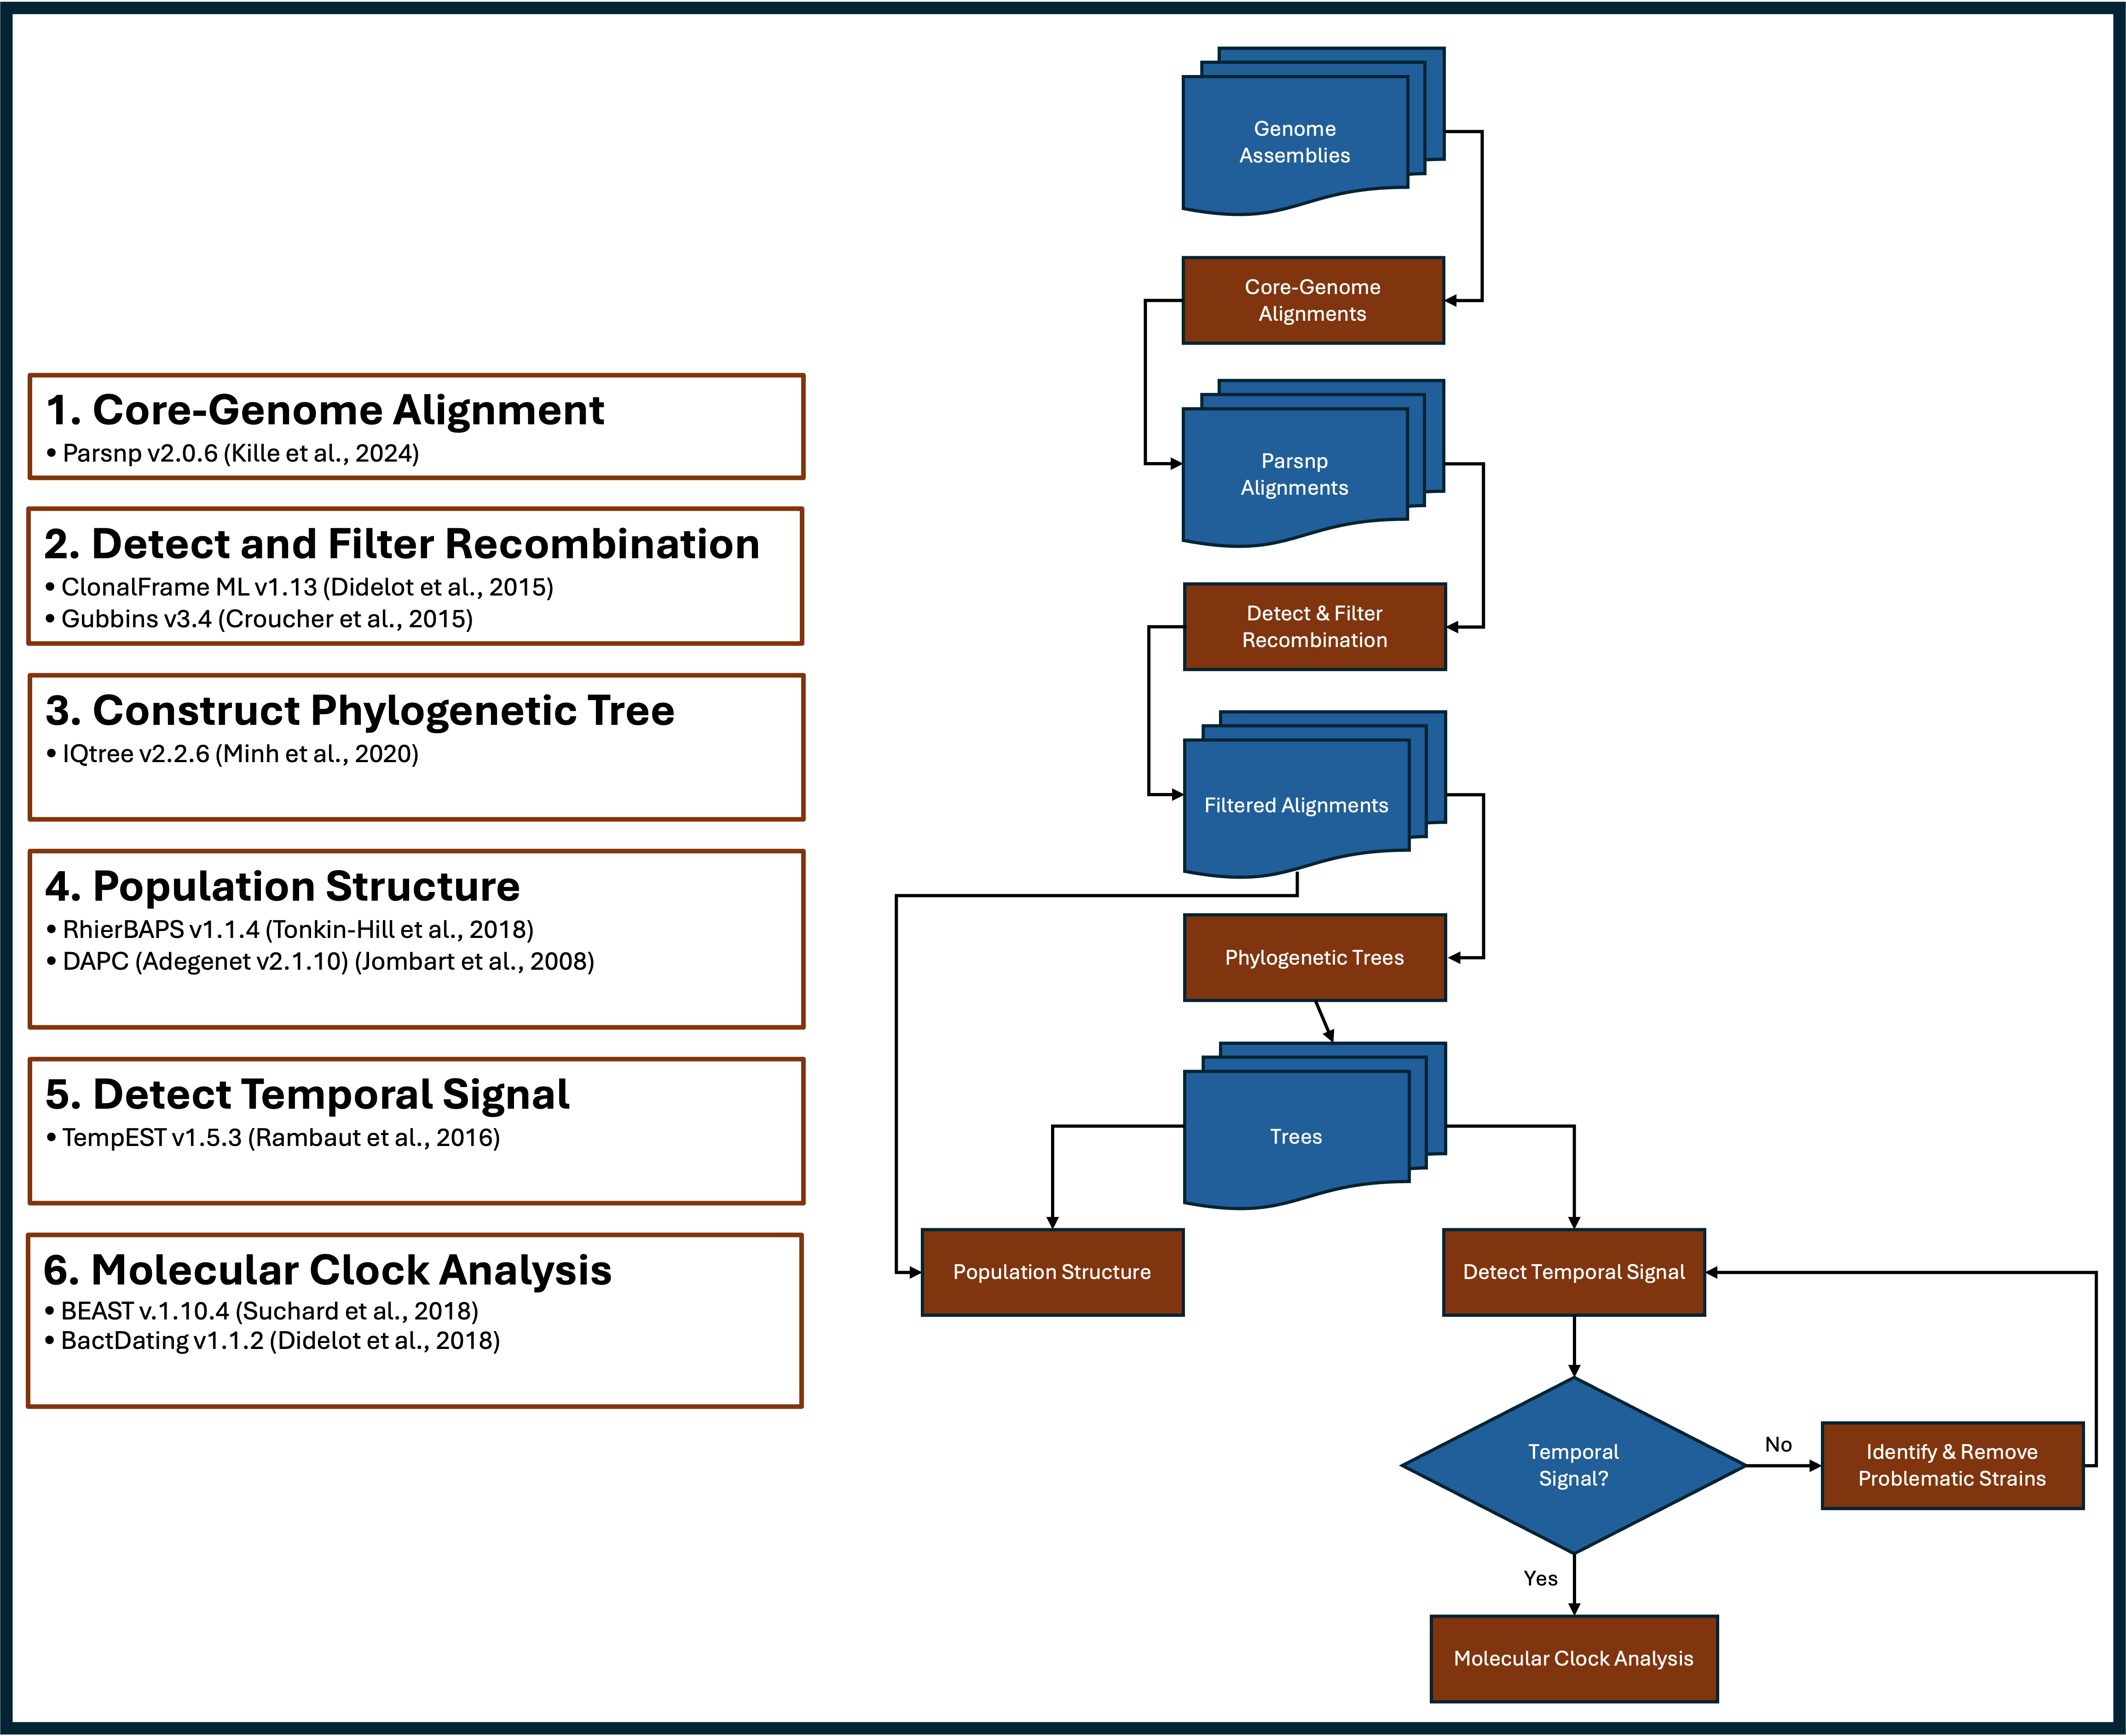
\includegraphics[width=0.8\linewidth,height=1\textheight]{Figures/Phylogentic_Workflow} 

}

\caption{Phylogenetic workflow}\label{fig:PhyloWorkflow}
\end{figure}

\subsection{Core-Genome Alignments}\label{core-genome-alignments}

I downloaded \texttt{Parsnp\ v2.0.6} (\citet{Kille2024}) to perform whole-genome core alignments. I used IVIA 1317 as a reference for \emph{XaJ} and I used isolate 15-088 as the \emph{Xap} reference therefore, I did not need to supply it as one of the genomes (in the /bigdata/adaskaveglab/ashan007/Assembly\_Workflow\_PlatanusB/Step5\_Analyses/Genomic\_Resources/Genomes directory) since it is included in the trees. Other than the CA\_XAP and CA\_XAP\_and\_NCBI22 runs, the reference is IVIA 1317. I then used \texttt{HarvestTools\ v1.3} (\citet{Treangen2014}) to convert the \texttt{.xmfa} to \texttt{.aln} (fasta) and concatenate the Local Colinear Blocks (LCBs).

\begin{itemize}
\tightlist
\item
  I removed the IVIA 1317 genomes from: CA\_XAJ\_and\_NCBI26, CA\_XAJ\_XAP\_and\_NCBI\_XAJ\_XAP and CA\_XAJ\_XAP\_and\_NCBI\_XAJ\_XAP\_and\_Outgroup Genomes subdirectories.
\item
  I removed the 15-088 genome from: CA\_XAP\_and\_NCBI22 Genomes subdirectory.
\item
  I also modified the \texttt{.aln} files to remove \texttt{.fa}, \texttt{.fna}, \texttt{.gbk}, or \texttt{.gbk.fna} extension in the sample name using \texttt{awk}. This code was applied to all runs:
\end{itemize}

\begin{Shaded}
\begin{Highlighting}[]
      \FunctionTok{awk} \StringTok{\textquotesingle{}/\^{}\textgreater{}/ \{ sub(/\textbackslash{}.gbk\textbackslash{}.fna$/, ""); sub(/\textbackslash{}.gbk$/, ""); sub(/\textbackslash{}.fna$/, ""); sub(/\textbackslash{}.fa$/, ""); \} 1\textquotesingle{}}\NormalTok{ CA\_XAJ.LCBs.aln }\OperatorTok{\textgreater{}}\NormalTok{ CA\_XAJ.LCBs.fasta}
\end{Highlighting}
\end{Shaded}

\begin{itemize}
\tightlist
\item
  I then checked it see if the sample names were correctly renamed using \texttt{grep} + \texttt{sed}:
\end{itemize}

\begin{Shaded}
\begin{Highlighting}[]
      \FunctionTok{grep} \StringTok{\textquotesingle{}\^{}\textgreater{}\textquotesingle{}}\NormalTok{ CA\_XAJ.LCBs.fasta }\KeywordTok{|} \FunctionTok{sed} \StringTok{\textquotesingle{}s/\^{}\textgreater{}//\textquotesingle{}} \OperatorTok{\textgreater{}}\NormalTok{ CA\_XAJ.LCBs.names.txt }
\end{Highlighting}
\end{Shaded}

\textbf{Scripts}

I used \texttt{Parsnp\_Final.sh} (\ref{Parsnp-script}) to generate the initial alignments and \texttt{HarvestTools\_Final.sh} (\ref{Harvest-script}) to extract the LCBs.

\subsection{Detect and Filter Recombination}\label{detect-and-filter-recombination}

\texttt{Gubbins\ v3.4} (\citet{croucher2015}) and \texttt{ClonalFrameML\ v1.13} (\citet{didelot2015}) (CFML) are two commonly used programs to detect and filter bacterial recombination. In order to produce accurate phylogenies we must account for recombination. I will use these two methods and compare the results (e.g.~core-genome alignments) using \texttt{AMAS} (\citet{borowiec2016}).

\textbf{Relevant Literature Phylogentetic Analyses}

\begin{itemize}
\tightlist
\item
  Parsnp + ClonalFrameML

  \begin{itemize}
  \tightlist
  \item
    Emergence of linezolid-resistant \emph{Enterococcus faecium} in a tertiary hospital in Copenhagen (2023) (\url{https://doi.org/10.1099/mgen.0.001055})
  \item
    Emergence and spread of \emph{Mycobacterium ulcerans} at different geographic scales (2024) (\url{https://journals.asm.org/doi/full/10.1128/spectrum.03827-23})
  \item
    Whole genome sequencing for investigations of meningococcal outbreaks in the United States: a retrospective analysis (2018) (\url{https://doi.org/10.1038/s41598-018-33622-5})
  \item
    Acquisition and dissemination of cephalosporin-resistant \emph{E. coli} in migratory birds sampled at an Alaska landfill as inferred through genomic analysis (2018) (\url{https://doi.org/10.1038/s41598-018-25474-w})
  \item
    The Green Revolution shaped the population structure of the rice pathogen \emph{Xanthomonas oryzae} pv. \emph{oryzae} (2020) (\url{https://doi.org/10.1038/s41396-019-0545-2})
  \item
    Evolutionary and epidemiological insights from historical and modern genomes of \emph{Xanthomonas oryzae} pv. \emph{oryzicola}, the causal agent of bacterial leaf streak of rice (2024) (\url{https://doi.org/10.1094/MPMI-05-24-0062-SC})
  \end{itemize}
\item
  Parsnp + Gubbins

  \begin{itemize}
  \tightlist
  \item
    Genomic Traits Associated with Virulence and Antimicrobial Resistance of Invasive Group B Streptococcus Isolates with Reduced Penicillin Susceptibility from Elderly Adults (2022) (\url{https://doi.org/10.1128/spectrum.00568-22})
  \item
    Population genomics and pathotypic evaluation of the bacterial leaf blight pathogen of rice reveals rapid evolutionary dynamics of a plant pathogen (2023) (\url{https://doi.org/10.3389/fcimb.2023.1183416})
  \item
    Natural Recombination among Type I Restriction-Modification Systems Creates Diverse Genomic Methylation Patterns among \emph{Xylella fastidiosa} Strains (2023) (\url{https://doi.org/10.1128/aem.01873-22})
  \item
    Genomic analysis of the multi-host pathogen \emph{Erysipelothrix rhusiopathiae} reveals extensive recombination as well as the existence of three generalist clades with wide geographic distribution (2016) (\url{https://doi.org/10.1186/s12864-016-2643-0})
  \item
    Global phylogenomic analyses of \emph{Mycobacterium abscessus} provide context for non cystic fibrosis infections and the evolution of antibiotic resistance (2021) (\url{https://doi.org/10.1038/s41467-021-25484-9})
  \end{itemize}
\end{itemize}

\subsection{Phylogenetic Tree}\label{phylogenetic-tree}

\texttt{IQtree2\ v.2.2.6} (\citet{Minh2020}) will be used to generate the phylogenetic tree based on the recombination-filtered genome alignments from \texttt{CFML} and \texttt{Gubbins}. Prior to generating the tree I ran \texttt{ModelFinder} (\citet{Kalyaanamoorthy2017}) to determine the optimal substitution model based on the alignments (Table \ref{tab:ModelF}). I compared the trees generated by \texttt{IQtree} + \texttt{Gubbins} and \texttt{IQtree} + \texttt{ClonalFrameML} using TreeCMP (\citet{goluch2020}).

\textbf{Models determined by ModelFinder}

The models are found within the \texttt{MFout.iqtree} file in the respective Parsnp run subdirectories, for example:

\begin{verbatim}
/bigdata/adaskaveglab/ashan007/Assembly_Workflow_PlatanusB/Step5_Analyses/IQtree2/Parsnp_CFML/CA_XAJ/ModelFinder

/bigdata/adaskaveglab/ashan007/Assembly_Workflow_PlatanusB/Step5_Analyses/IQtree2/Parsnp_Gubbins/CA_XAJ/ModelFinder
\end{verbatim}

\begin{longtable}[]{@{}
  >{\centering\arraybackslash}p{(\columnwidth - 6\tabcolsep) * \real{0.2500}}
  >{\centering\arraybackslash}p{(\columnwidth - 6\tabcolsep) * \real{0.2500}}
  >{\centering\arraybackslash}p{(\columnwidth - 6\tabcolsep) * \real{0.2500}}
  >{\centering\arraybackslash}p{(\columnwidth - 6\tabcolsep) * \real{0.2500}}@{}}
\caption{\label{tab:ModelF} Models determined by \texttt{ModelFinder.}}\tabularnewline
\toprule\noalign{}
\begin{minipage}[b]{\linewidth}\centering
\textbf{Run}
\end{minipage} & \begin{minipage}[b]{\linewidth}\centering
\textbf{ClonalFrameML}
\end{minipage} & \begin{minipage}[b]{\linewidth}\centering
\textbf{Gubbins}
\end{minipage} & \begin{minipage}[b]{\linewidth}\centering
\textbf{Outgroup}
\end{minipage} \\
\midrule\noalign{}
\endfirsthead
\toprule\noalign{}
\begin{minipage}[b]{\linewidth}\centering
\textbf{Run}
\end{minipage} & \begin{minipage}[b]{\linewidth}\centering
\textbf{ClonalFrameML}
\end{minipage} & \begin{minipage}[b]{\linewidth}\centering
\textbf{Gubbins}
\end{minipage} & \begin{minipage}[b]{\linewidth}\centering
\textbf{Outgroup}
\end{minipage} \\
\midrule\noalign{}
\endhead
\bottomrule\noalign{}
\endlastfoot
CA\_XAJ & HKY+F+I & HKY+F+I & NONE \\
CA\_XAJ\_and\_NCBI26 & TPM3u+F+I & TPM3u+F+I & NONE \\
CA\_XAJ\_XAP\_and\_NCBI\_XAJ\_XAP & TVM+F+I & GTR+F+I & NONE \\
CA\_XAJ\_XAP\_and\_NCBI\_XAJ\_XAP\_and\_Outgroup & TVM+F+I+G4 & GTR+F+I & JS749\_3 \\
CA\_XAJ\_XAP & HKY+F+I & GTR+F+I & NONE \\
CA\_XAJ\_and\_NCBI24 & HKY+F+I & HKY+F+I & NONE \\
CA\_XAP & K3Pu+F+I & K3Pu+F+I & NONE \\
\end{longtable}

\textbf{Scripts}
ClonalFrameML: ModelFinder and IQtree were ran using \texttt{IQTree2\_MF\_Parsnp\_CFML\_Final.sh} (\ref{MFCFML-script}) and \texttt{IQTree2\_Parsnp\_CFML\_Final.sh} (\ref{IQCFML-script}), respectively.\\
Gubbins: ModelFinder and IQtree were ran using \texttt{IQTree2\_MF\_Parsnp\_Gubbins\_Final.sh} (\ref{MFGUB-script}) and \texttt{IQTree2\_Gubbins\_Final.sh} (\ref{IQGUB-script}), respectively.

\subsection{Population Structure}\label{population-structure}

To complement and support the phylogenies, I wanted to elucidate the population structure using two methods: \texttt{RhierBAPS} (\citet{TonkinHill2018}) and DAPC (\citet{Jombart2008}). \texttt{RhierBAPS} is a Bayesian clustering approach and DAPC is a model-free approach that combined PCA (Principal Component Analysis) for dimensionality reduction and DA (Discriminant Analysis) to maximize the separation between pre-defined or inferred clusters.

First I ran RheirBAPS to generate the clusters based on the input recombination-filtered genome alignment and respective IQtree tree. The recombination-filtered genome alignment was converted into a SNP matrix then into a \texttt{genind} object in order to perform the DAPC. The clusters then served as the groups (\texttt{grp}) for the DAPC analysis.

\textbf{Scripts}:

I will only provide the scripts that we will likely use for the manuscripts.

Parsnp + CFML + IQtree

\begin{itemize}
\tightlist
\item
  CA\_XAJ: \texttt{CA\_XAJ\_hierBAPS.R}
\item
  CA\_XAJ\_115: \texttt{CA\_XAJ\_hierBAPS.R} ((\ref{CAXAJ115BAPS-script}))
\item
  CA\_XAJ\_115\_and\_NCBI24: \texttt{CA\_XAJ\_and\_NCBI24\_hierBAPS.R} ((\ref{CAXAJNCBI24BAPS-script}))
\item
  CA\_XAJ\_115\_and\_NCBI26: \texttt{CA\_XAJ\_and\_NCBI26\_hierBAPS.R}
\item
  CA\_XAJ\_115\_XAP: \texttt{CA\_XAJ\_hierBAPS.R}
\item
  CA\_XAJ\_115\_XAP\_and\_NCBI\_XAJ\_XAP: \texttt{CA\_XAJ\_XAP\_and\_NCBI\_XAJ\_XAP\_hierBAPS.R}
\item
  CA\_XAJ\_115\_XAP\_and\_NCBI\_XAJ\_XAP\_and\_Outgroup: \texttt{CA\_XAJ\_XAP\_and\_NCBI\_XAJ\_XAP\_and\_Outgroup\_hierBAPS.R} ((\ref{ALLBAPS-script}))
\item
  CA\_XAJ\_and\_NCBI24: \texttt{CA\_XAJ\_and\_NCBI24\_hierBAPS.R}
\item
  CA\_XAJ\_and\_NCBI26: \texttt{CA\_XAJ\_and\_NCBI26\_hierBAPS.R}
\item
  CA\_XAJ\_XAP: \texttt{CA\_XAJ\_XAP\_hierBAPS.R}
\item
  CA\_XAJ\_XAP\_and\_NCBI\_XAJ\_XAP: \texttt{CA\_XAJ\_XAP\_and\_NCBI\_XAJ\_XAP\_hierBAPS.R}
\item
  CA\_XAJ\_XAP\_and\_NCBI\_XAJ\_XAP\_and\_Outgroup: \texttt{CA\_XAJ\_XAP\_and\_NCBI\_XAJ\_XAP\_and\_Outgroup\_hierBAPS.R}
\item
  CA\_XAP: \texttt{CA\_XAP\_hierBAPS.R}
\item
  CA\_XAP\_and\_NCBI22: \texttt{CA\_XAP\_NCBI22\_hierBAPS.R}
\end{itemize}

\subsection{Molecular Clock}\label{molecular-clock}

I wanted to see if our data was `clock-like' and fit for a dated phylogenetic analysis. To determine if the data is `clock-like' you must detect a significant temporal signal by performing a root-to-tip regression analysis.

``A data set is considered to have temporal signal if it can be treated as a measurably evolving population, defined by \citet{Drummond2003} as ``populations from which molecular sequences can be taken at different points in time, among which there are a statistically significant number of genetic differences. (\citet{Duchene2020})''

If there is a weak temporal signal, then the data does not exhibit clock-like behavior and is unfit for molecular dating analysis.

I used two programs to detect temporal signal:

\begin{itemize}
\tightlist
\item
  \texttt{TempEST\ v1.5.3} (\citet{Rambaut2016})

  \begin{itemize}
  \item
    TempEst (short for ``Temporal Explorer of Sequence Trees,'' formerly known as Path-O-Gen) is a tool designed for analyzing the temporal signal and ``clocklikeness'' of molecular phylogenies. It's widely used in evolutionary biology to assess whether a dataset of genetic sequences (e.g., from viruses or bacteria) shows a measurable rate of evolution over time. TempEst can handle both contemporaneous trees (all sequences collected at the same time) and dated-tip trees (sequences collected at different times). It helps researchers visualize the relationship between genetic divergence and sampling dates through root-to-tip regression plots, and it can suggest an optimal root for the tree that aligns with a molecular clock assumption.
  \item
    Since \texttt{TempEST} is a stand-alone software package with a GUI, I do not have any associated code. I followed the tutorial described \href{https://beast.community/tempest_tutorial}{here}.
  \end{itemize}
\item
  \texttt{BactDating\ v1.1.2} (\citet{didelot2018})

  \begin{itemize}
  \tightlist
  \item
    BactDating is a Bayesian tool for dating ancestral nodes in bacterial phylogenetic trees, integrating molecular clock models with epidemiological or historical data. It's particularly useful for reconstructing the evolutionary history of bacterial pathogens, estimating when key events (like outbreaks or divergences) occurred. Built in R, it uses a relaxed molecular clock and can incorporate uncertainty in tip dates (sampling times), making it flexible for messy real-world datasets.
  \end{itemize}
\end{itemize}

I performed temporal analysis using \texttt{BactDating} on the CA\_XAJ and CA\_XAJ\_and\_NCBI24 runs using the following data and scripts:

\begin{itemize}
\tightlist
\item
  ClonalFrameML output

  \begin{itemize}
  \tightlist
  \item
    CA\_XAJ script: \texttt{CA\_XAJ\_CFML\_BactDating.R} (\ref{BDCFML-script})
  \item
    CA\_XAJ\_and\_NCBI24 script: \texttt{CA\_XAJ\_NCBI24\_CFML\_BactDating.R}
  \end{itemize}
\item
  Gubbins output

  \begin{itemize}
  \tightlist
  \item
    CA\_XAJ script: \texttt{CA\_XAJ\_Gub\_BactDating.R} (\ref{BDGUB-script})
  \item
    CA\_XAJ\_and\_NCBI24 script: \texttt{CA\_XAJ\_NCBI24\_Gub\_BactDating.R}
  \end{itemize}
\item
  IQtree2 tree based on the CFML-filtered alignment

  \begin{itemize}
  \tightlist
  \item
    CA\_XAJ script: \texttt{CA\_XAJ\_CFML\_IQtree\_BactDating.R} (\ref{BDIQCFML-script})
  \item
    CA\_XAJ\_and\_NCBI24 script: \texttt{CA\_XAJ\_NCBI24\_CFML\_IQtree\_BactDating.R}
  \end{itemize}
\item
  IQtree2 tree based on the Gubbins-filtered alignment

  \begin{itemize}
  \tightlist
  \item
    CA\_XAJ script: \texttt{CA\_XAJ\_Gub\_IQtree\_BactDating.R} (\ref{BDIQGUB-script})
  \item
    CA\_XAJ\_and\_NCBI24 script: \texttt{CA\_XAJ\_NCBI24\_Gub\_IQtree\_BactDating.R}
  \end{itemize}
\end{itemize}

\textbf{NOTE}: I only provided one example for each of the data because the code is the same for the runs.

\section{Type III Effectors}\label{T3EMeth}

I downloaded Xanthomonas type III secretion system effectors (T3E) (n= 76) (Accessed July 19, 2024) from \href{https://euroxanth.ipn.pt/doku.php?id=bacteria:t3e:t3e}{Euroxanth} to serve as BLAST reference/queries for BlastP and tBLASTn against our CA Xaj and Xap populations. See \texttt{Xanthomonas\_Effectors.xlsx} for more information on these reference T3Es and the preliminary results.

This work was performed on the HPCC in the following directory:

\begin{verbatim}
/bigdata/adaskaveglab/ashan007/Assembly_Workflow_PlatanusB/Step5_Analyses/Effectors
\end{verbatim}

\textbf{BLAST}

\begin{itemize}
\item
  tBLASTn was ran using \texttt{Xaj\_Xap\_T3SSE\_tBLASTn.sh} (\ref{tblastn-script})
\item
  BLASTp was ran using \texttt{Xaj\_Xap\_T3SSE\_BLASTp.sh} (\ref{blastp-script})
\item
  Both BLASTp and tBLASTn had these settings:

\begin{verbatim}
-evalue 1e-10
-num_threads 8
-max_target_seqs 5
-max_hsps 5 
\end{verbatim}
\item
  Both the .txt and alignment outputs were generated.
\end{itemize}

\subsubsection{Method 1}\label{method-1}

\textbf{\citet{Subedi2024}}

``The presence of 72 T3Es (Supplementary Table S2) was investigated for all genomes using tBLASTn with E-value greater than 10--5. A threshold of \textgreater{} 80\% amino acid identity covering \textgreater80\% of query length was considered as the presence of an effector.'' with the addition of BLASTp using the same filtering criteria.

\textbf{Steps:}

\begin{enumerate}
\def\labelenumi{\arabic{enumi}.}
\tightlist
\item
  Run tBLASTn using \texttt{Xaj\_Xap\_T3SSE\_tBLASTn.sh} (\ref{tblastn-script}).
\item
  Filter the tBLASTn output for effectors using a threshold of \textgreater{} 80\% amino acid identity covering \textgreater{} 80\% of query length using \texttt{Filter\_tBLASTn.py} (\ref{filtertblastn-script}).
\item
  Identify duplicate hits for qseqid and remove the hits with a lower percent ID (my modification) using \texttt{Filter\_tBLASTn.RemoveDups.py} (\ref{reduptblastn-script}).
\item
  Generate a presence/absence matrix using \texttt{BLAST\_Matrix\_FamilyName.method1.py} (\ref{mxfnmeth1-script}) and \texttt{BLAST\_Matrix\_RefSeqID.method1.py} (\ref{mxrsmeth1-script}).
\end{enumerate}

\subsubsection{Method 2}\label{method-2}

\textbf{\citet{Fernandes2021}}

``The genome sequences of the four Xanthomonas strains used in this study were scrutinized for the presence of protein homologs by tBLASTn analysis (tBLASTn v. 2.10.1 ) against a created database of protein sequences previously reported to be involved in the pathogenesis and virulence of Xanthomonas (Table S3). To ensure that only closely-related orthologous proteins were selected, the tBLASTn cut-offs criteria to identify protein homologs were \(\geq 40\)\% identity and \(\geq 75\)\% query sequence length.''

\textbf{Steps:}

\begin{enumerate}
\def\labelenumi{\arabic{enumi}.}
\tightlist
\item
  Run tBLASTn using \texttt{Xaj\_Xap\_T3SSE\_tBLASTn.sh} (\ref{tblastn-script}).
\item
  Filter the tBLASTn output for effectors using a threshold of \(\geq 40\)\% identity and \(\geq 75\)\% query sequence length using \texttt{Filter\_tBLASTn.v2.py} (\ref{filtertblastn2-script}).
\item
  Identify duplicate hits for qseqid and remove the hits with a lower percent ID (my modification) using \texttt{Filter\_tBLASTn.RemoveDups.py} (\ref{reduptblastn-script}).
\item
  Generate a presence/absence matrix using \texttt{BLAST\_Matrix\_FamilyName.method2.py} (\ref{mxfnmeth2-script}) and \texttt{BLAST\_Matrix\_RefSeqID.method2.py} (\ref{mxrsmeth2-script}).
\end{enumerate}

\subsubsection{Method 3}\label{method-3}

\textbf{\citet{assis2021}}

``A set of 63 type III effectors from the Xanthomonas Resource \href{http://www.xanthomonas.org/tools.html}{website} was analyzed by protein-nucleotide six-frame translation (tBlastn) searches {[}74{]} with E-value 1e-50 against the set of 32 Xaj genomes.''

\textbf{Steps:}

\begin{enumerate}
\def\labelenumi{\arabic{enumi}.}
\tightlist
\item
  Run tBLASTn using \texttt{Xaj\_Xap\_T3SSE\_tBLASTn.sh} (\ref{tblastn-script}).
\item
  Filter the tBLASTn output for effectors using a threshold of E-value \(\leq 1e-50\) using \texttt{Filter\_tBLASTn.v3.py} (\ref{filtertblastn3-script}).
\item
  Generate a presence/absence matrix using \texttt{BLAST\_Matrix\_FamilyName.v2.py} (\ref{mxfn2-script}) and \texttt{BLAST\_Matrix\_RefSeqID.v2.py} (\ref{mxrs2-script}).
\end{enumerate}

\subsubsection{Method 4}\label{method-4}

Inspecting the PPanGGoLiN data matrix for the presence of annotated T3Es.

\begin{itemize}
\tightlist
\item
  (CA\_XAJ\_XAP run: CA\_XAJ\_XAP\_PPanGGOLiN\_Matrix.xlsx)
\item
  (CA\_XAJ\_115 run: matrix\_Xaj\_115.xlsx)
\end{itemize}

\textbf{Steps}

\begin{enumerate}
\def\labelenumi{\arabic{enumi}.}
\tightlist
\item
  CA\_XAJ\_XAP\_PPanGGOLiN\_Matrix.xlsx was used to identify effectors by name and then by searching for genes present in method 3 by gene ID to identify those genes in the PPanGGOLiN results.
\item
  for select genes I took a representative sequence from one strain and performed a web-based BLASTp to confirm that the protein is the respective effector. See Note 4 on the Preliminary\_Results tab of \texttt{Xanthomonas\_Effectors.xlsx}.
\end{enumerate}

\chapter{Results}\label{Results}

\section{Read Processing}\label{read-processing-1}

On average, 3.92 ± 0.44 G of raw data was generated for each strain (Table \ref{tab:SeqRes}).

\begin{longtable}[]{@{}
  >{\centering\arraybackslash}p{(\columnwidth - 14\tabcolsep) * \real{0.1250}}
  >{\centering\arraybackslash}p{(\columnwidth - 14\tabcolsep) * \real{0.1250}}
  >{\centering\arraybackslash}p{(\columnwidth - 14\tabcolsep) * \real{0.1250}}
  >{\centering\arraybackslash}p{(\columnwidth - 14\tabcolsep) * \real{0.1250}}
  >{\centering\arraybackslash}p{(\columnwidth - 14\tabcolsep) * \real{0.1250}}
  >{\centering\arraybackslash}p{(\columnwidth - 14\tabcolsep) * \real{0.1250}}
  >{\centering\arraybackslash}p{(\columnwidth - 14\tabcolsep) * \real{0.1250}}
  >{\centering\arraybackslash}p{(\columnwidth - 14\tabcolsep) * \real{0.1250}}@{}}
\caption{\label{tab:SeqRes} Sequencing results from Novogene.}\tabularnewline
\toprule\noalign{}
\begin{minipage}[b]{\linewidth}\centering
\textbf{Sample}
\end{minipage} & \begin{minipage}[b]{\linewidth}\centering
\textbf{Raw reads}
\end{minipage} & \begin{minipage}[b]{\linewidth}\centering
\textbf{Raw data}
\end{minipage} & \begin{minipage}[b]{\linewidth}\centering
\textbf{Effective(\%)}
\end{minipage} & \begin{minipage}[b]{\linewidth}\centering
\textbf{Error(\%)}
\end{minipage} & \begin{minipage}[b]{\linewidth}\centering
\textbf{Q20(\%)}
\end{minipage} & \begin{minipage}[b]{\linewidth}\centering
\textbf{Q30(\%)}
\end{minipage} & \begin{minipage}[b]{\linewidth}\centering
\textbf{GC(\%)}
\end{minipage} \\
\midrule\noalign{}
\endfirsthead
\toprule\noalign{}
\begin{minipage}[b]{\linewidth}\centering
\textbf{Sample}
\end{minipage} & \begin{minipage}[b]{\linewidth}\centering
\textbf{Raw reads}
\end{minipage} & \begin{minipage}[b]{\linewidth}\centering
\textbf{Raw data}
\end{minipage} & \begin{minipage}[b]{\linewidth}\centering
\textbf{Effective(\%)}
\end{minipage} & \begin{minipage}[b]{\linewidth}\centering
\textbf{Error(\%)}
\end{minipage} & \begin{minipage}[b]{\linewidth}\centering
\textbf{Q20(\%)}
\end{minipage} & \begin{minipage}[b]{\linewidth}\centering
\textbf{Q30(\%)}
\end{minipage} & \begin{minipage}[b]{\linewidth}\centering
\textbf{GC(\%)}
\end{minipage} \\
\midrule\noalign{}
\endhead
\bottomrule\noalign{}
\endlastfoot
XAJ1028 & 25591934 & 3.8 & 99.8 & 0.03 & 97.84 & 94.32 & 65.61 \\
XAJ1046 & 27128744 & 4.1 & 99.78 & 0.03 & 97.84 & 94.33 & 65.62 \\
XAJ1048 & 22783072 & 3.4 & 99.78 & 0.02 & 97.91 & 94.49 & 65.53 \\
XAJ1049 & 24548562 & 3.7 & 99.72 & 0.02 & 97.91 & 94.51 & 65.47 \\
XAJ1054 & 21141570 & 3.2 & 99.4 & 0.03 & 97 & 93.14 & 65.35 \\
XAJ1082 & 23517808 & 3.5 & 99.79 & 0.02 & 97.92 & 94.52 & 65.58 \\
XAJ1086 & 22371990 & 3.4 & 99.79 & 0.02 & 97.96 & 94.58 & 65.6 \\
XAJ1148 & 25554480 & 3.8 & 99.79 & 0.02 & 97.96 & 94.6 & 65.53 \\
XAJ1149 & 24621852 & 3.7 & 99.81 & 0.02 & 97.86 & 94.42 & 65.59 \\
XAJ1197 & 26704772 & 4 & 99.82 & 0.03 & 97.79 & 94.26 & 65.48 \\
XAJ1213 & 22911558 & 3.4 & 99.83 & 0.02 & 97.88 & 94.38 & 65.46 \\
XAJ1239 & 28284048 & 4.2 & 99.82 & 0.03 & 97.77 & 94.2 & 65.54 \\
XAJ1246 & 24498244 & 3.7 & 99.82 & 0.02 & 97.92 & 94.46 & 65.49 \\
XAJ1250 & 27743394 & 4.2 & 99.85 & 0.02 & 97.92 & 94.52 & 65.48 \\
XAJ1395 & 23141436 & 3.5 & 99.78 & 0.02 & 98.2 & 95.06 & 65.49 \\
XAJ1399 & 23736590 & 3.6 & 99.7 & 0.02 & 98.12 & 94.94 & 65.49 \\
XAJ145 & 30305706 & 4.5 & 99.79 & 0.03 & 97.7 & 93.98 & 65.55 \\
XAJ1498 & 22844534 & 3.4 & 99.73 & 0.02 & 98.11 & 94.9 & 65.54 \\
XAJ1535 & 20554072 & 3.1 & 99.73 & 0.02 & 97.95 & 94.38 & 60.1 \\
XAJ1537 & 28392148 & 4.3 & 99.75 & 0.02 & 98.14 & 94.97 & 65.47 \\
XAJ1539 & 25641200 & 3.8 & 99.77 & 0.02 & 98.1 & 94.88 & 65.54 \\
XAJ1551 & 24648774 & 3.7 & 99.76 & 0.02 & 98.17 & 95.03 & 65.63 \\
XAJ1554 & 24667592 & 3.7 & 99.81 & 0.02 & 98.12 & 94.93 & 65.64 \\
XAJ1556 & 26642296 & 4 & 99.77 & 0.02 & 98.11 & 94.91 & 65.53 \\
XAJ1557 & 32063060 & 4.8 & 99.74 & 0.02 & 98.18 & 95.03 & 65.48 \\
XAJ1558 & 22755570 & 3.4 & 99.79 & 0.02 & 98.16 & 94.97 & 65.5 \\
XAJ1595 & 26746834 & 4 & 99.8 & 0.03 & 97.8 & 94.17 & 65.51 \\
XAJ1606 & 22419850 & 3.4 & 99.83 & 0.02 & 97.95 & 94.57 & 65.48 \\
XAJ1613 & 27831348 & 4.2 & 99.79 & 0.03 & 97.79 & 94.18 & 65.4 \\
XAJ1614 & 27277774 & 4.1 & 99.8 & 0.03 & 97.75 & 94.1 & 65.53 \\
XAJ1615 & 26327478 & 3.9 & 99.8 & 0.02 & 97.86 & 94.34 & 65.34 \\
XAJ1616 & 30127594 & 4.5 & 99.82 & 0.03 & 97.77 & 94.12 & 65.55 \\
XAJ1617 & 27929602 & 4.2 & 99.8 & 0.03 & 97.77 & 94.11 & 65.62 \\
XAJ1626 & 26635082 & 4 & 99.78 & 0.03 & 97.81 & 94.21 & 65.52 \\
XAJ163 & 27523144 & 4.1 & 99.81 & 0.02 & 97.88 & 94.37 & 65.5 \\
XAJ165 & 29565610 & 4.4 & 99.83 & 0.03 & 97.69 & 93.98 & 65.5 \\
XAJ169 & 29377416 & 4.4 & 99.83 & 0.03 & 97.82 & 94.24 & 65.5 \\
XAJ1710 & 23142910 & 3.5 & 99.81 & 0.03 & 97.74 & 94.07 & 65.41 \\
XAJ1711 & 25659456 & 3.8 & 99.81 & 0.03 & 97.75 & 94.09 & 65.36 \\
XAJ1808 & 26157004 & 3.9 & 99.84 & 0.03 & 97.61 & 93.78 & 65.55 \\
XAJ181 & 30304682 & 4.5 & 99.83 & 0.03 & 97.75 & 94.07 & 65.49 \\
XAJ1822 & 25639610 & 3.8 & 99.84 & 0.03 & 97.65 & 93.89 & 65.51 \\
XAJ1824 & 27202276 & 4.1 & 99.83 & 0.03 & 97.83 & 94.25 & 65.53 \\
XAJ2122 & 29431940 & 4.4 & 99.77 & 0.02 & 97.89 & 94.38 & 65.52 \\
XAJ2124 & 24947322 & 3.7 & 99.85 & 0.02 & 97.87 & 94.33 & 65.32 \\
XAJ2125 & 21836920 & 3.3 & 99.79 & 0.03 & 97.77 & 94.18 & 65.32 \\
XAJ2128 & 27026812 & 4.1 & 99.87 & 0.02 & 97.9 & 94.44 & 65.25 \\
XAJ2129 & 28275218 & 4.2 & 99.86 & 0.02 & 97.91 & 94.48 & 65.29 \\
XAJ2131 & 29505070 & 4.4 & 99.82 & 0.03 & 97.81 & 94.27 & 65.46 \\
XAJ2165 & 16555726 & 2.5 & 99.74 & 0.02 & 97.9 & 94.48 & 65.35 \\
XAJ2167 & 27266132 & 4.1 & 99.84 & 0.02 & 97.89 & 94.46 & 65.28 \\
XAJ2169 & 26778130 & 4 & 99.85 & 0.02 & 97.98 & 94.59 & 64.07 \\
XAJ2170 & 23357712 & 3.5 & 99.85 & 0.03 & 97.79 & 94.22 & 65.4 \\
XAJ2178 & 25383038 & 3.8 & 99.82 & 0.02 & 97.9 & 94.48 & 65.4 \\
XAJ2180 & 25701552 & 3.9 & 99.79 & 0.02 & 97.86 & 94.37 & 65.58 \\
XAJ283A & 31719184 & 4.8 & 99.75 & 0.03 & 97.76 & 94.14 & 65.55 \\
XAJ283B & 23850040 & 3.6 & 99.58 & 0.02 & 97.86 & 94.35 & 65.53 \\
XAJ30 & 28549684 & 4.3 & 99.83 & 0.03 & 97.85 & 94.28 & 65.68 \\
XAJ31 & 30944874 & 4.6 & 99.79 & 0.03 & 97.65 & 93.89 & 65.69 \\
XAJ32 & 26826246 & 4 & 99.83 & 0.03 & 97.67 & 93.92 & 65.39 \\
XAJ321 & 28989620 & 4.3 & 99.83 & 0.03 & 97.73 & 94.05 & 65.36 \\
XAJ322 & 29391010 & 4.4 & 99.64 & 0.03 & 97.61 & 93.81 & 65.52 \\
XAJ33 & 29806428 & 4.5 & 99.56 & 0.03 & 97.28 & 93.22 & 65.51 \\
XAJ330 & 25695714 & 3.9 & 99.8 & 0.03 & 97.71 & 94.01 & 65.48 \\
XAJ333 & 25529262 & 3.8 & 99.74 & 0.03 & 97.83 & 94.28 & 65.46 \\
XAJ338 & 29804220 & 4.5 & 99.76 & 0.02 & 97.92 & 94.46 & 65.51 \\
XAJ34 & 22366134 & 3.4 & 99.85 & 0.03 & 97.74 & 94.08 & 65.42 \\
XAJ340 & 30453802 & 4.6 & 99.82 & 0.02 & 97.9 & 94.44 & 65.43 \\
XAJ341 & 22967944 & 3.4 & 99.76 & 0.03 & 97.72 & 94.21 & 64.7 \\
XAJ344 & 32172478 & 4.8 & 99.81 & 0.03 & 97.84 & 94.33 & 65.16 \\
XAJ345 & 26215790 & 3.9 & 99.81 & 0.03 & 97.85 & 94.33 & 65.5 \\
XAJ347 & 23904350 & 3.6 & 99.56 & 0.02 & 98.23 & 95.18 & 65.32 \\
XAJ349 & 24222738 & 3.6 & 99.5 & 0.02 & 98.21 & 95.12 & 65.46 \\
XAJ35 & 30751938 & 4.6 & 99.8 & 0.03 & 97.65 & 93.84 & 65.49 \\
XAJ355 & 26167538 & 3.9 & 99.76 & 0.03 & 97.81 & 94.24 & 65.4 \\
XAJ36 & 25042538 & 3.8 & 99.8 & 0.03 & 97.72 & 94.04 & 65.63 \\
XAJ372 & 26460434 & 4 & 99.72 & 0.02 & 98.05 & 94.71 & 65.5 \\
XAJ38 & 34529828 & 5.2 & 99.81 & 0.03 & 97.69 & 93.95 & 65.47 \\
XAJ390 & 28702950 & 4.3 & 99.81 & 0.03 & 97.78 & 94.21 & 65.59 \\
XAJ402 & 24876514 & 3.7 & 99.77 & 0.02 & 97.93 & 94.53 & 65.48 \\
XAJ426 & 25297070 & 3.8 & 99.79 & 0.03 & 97.74 & 94.1 & 65.46 \\
XAJ427 & 22565974 & 3.4 & 99.81 & 0.02 & 98.05 & 94.72 & 64.6 \\
XAJ428 & 24115680 & 3.6 & 99.75 & 0.02 & 98.18 & 95.05 & 65.51 \\
XAJ432 & 24746174 & 3.7 & 99.78 & 0.02 & 98.17 & 95.03 & 65.52 \\
XAJ435 & 22312592 & 3.3 & 99.77 & 0.02 & 98.16 & 94.97 & 65.45 \\
XAJ438 & 25001438 & 3.8 & 99.78 & 0.02 & 98.19 & 95.05 & 65.51 \\
XAJ439 & 23152004 & 3.5 & 99.75 & 0.02 & 98.15 & 94.95 & 65.5 \\
XAJ456 & 25371674 & 3.8 & 99.78 & 0.02 & 98.26 & 95.21 & 65.56 \\
XAJ458 & 24367088 & 3.7 & 99.73 & 0.02 & 98.04 & 94.73 & 65.57 \\
XAJ462 & 25507154 & 3.8 & 99.77 & 0.02 & 98.11 & 94.9 & 65.52 \\
XAJ464 & 25831450 & 3.9 & 99.12 & 0.02 & 97.89 & 94.37 & 65.61 \\
XAJ465 & 22375006 & 3.4 & 99.67 & 0.02 & 98.09 & 94.85 & 65.6 \\
XAJ466 & 24006834 & 3.6 & 99.64 & 0.02 & 98.06 & 94.8 & 65.59 \\
XAJ467 & 24139960 & 3.6 & 99.68 & 0.02 & 98.16 & 95.03 & 65.59 \\
XAJ469 & 25378860 & 3.8 & 99.82 & 0.02 & 97.98 & 94.58 & 65.63 \\
XAJ470 & 26132060 & 3.9 & 99.76 & 0.02 & 97.92 & 94.5 & 65.62 \\
XAJ473 & 27096368 & 4.1 & 99.79 & 0.03 & 97.75 & 94.07 & 65.65 \\
XAJ476 & 32787634 & 4.9 & 99.74 & 0.02 & 97.94 & 94.52 & 65.63 \\
XAJ477 & 27245078 & 4.1 & 99.81 & 0.02 & 97.96 & 94.57 & 65.67 \\
XAJ669 & 23070940 & 3.5 & 99.8 & 0.02 & 98.09 & 94.78 & 65.47 \\
XAJ670 & 26035570 & 3.9 & 99.74 & 0.02 & 97.93 & 94.52 & 65.61 \\
XAJ671 & 28669172 & 4.3 & 99.74 & 0.02 & 97.97 & 94.57 & 65.56 \\
XAJ672 & 24008700 & 3.6 & 99.75 & 0.02 & 97.9 & 94.4 & 65.43 \\
XAJ673 & 26955266 & 4 & 99.76 & 0.03 & 97.82 & 94.25 & 65.44 \\
XAJ674 & 26455670 & 4 & 99.77 & 0.03 & 97.82 & 94.26 & 65.61 \\
XAJ675 & 23235694 & 3.5 & 99.78 & 0.02 & 97.87 & 94.37 & 65.63 \\
XAJ729 & 26190522 & 3.9 & 99.77 & 0.02 & 98.03 & 94.72 & 65.53 \\
XAJ730 & 28142470 & 4.2 & 99.77 & 0.02 & 97.91 & 94.5 & 65.41 \\
XAJ731 & 35859524 & 5.4 & 99.74 & 0.03 & 97.82 & 94.28 & 65.51 \\
XAJ929 & 26992496 & 4 & 99.72 & 0.02 & 97.86 & 94.41 & 65.57 \\
XAJ930 & 24434222 & 3.7 & 99.74 & 0.02 & 97.98 & 94.59 & 65.54 \\
XAJ934 & 26225454 & 3.9 & 99.78 & 0.02 & 97.94 & 94.55 & 65.57 \\
XAJ935 & 25156038 & 3.8 & 99.72 & 0.02 & 97.86 & 94.41 & 65.58 \\
XAJ936 & 21308058 & 3.2 & 99.76 & 0.02 & 97.91 & 94.49 & 65.57 \\
XAJ939 & 25645362 & 3.8 & 99.81 & 0.03 & 97.8 & 94.23 & 65.42 \\
XAJ940 & 27863848 & 4.2 & 99.77 & 0.02 & 97.94 & 94.5 & 65.35 \\
XAJ968 & 21680944 & 3.3 & 99.8 & 0.02 & 97.87 & 94.41 & 65.64 \\
XAJ969 & 22272334 & 3.3 & 99.74 & 0.03 & 97.83 & 94.32 & 65.59 \\
XAJ973 & 23804496 & 3.6 & 99.56 & 0.03 & 97.76 & 94.16 & 65.49 \\
XAJ984 & 21104792 & 3.2 & 98.65 & 0.03 & 96.53 & 92.82 & 65.19 \\
XAP1007 & 23944430 & 3.6 & 99.8 & 0.02 & 98.05 & 94.72 & 65.71 \\
XAP1010 & 27496956 & 4.1 & 99.82 & 0.02 & 98.13 & 94.92 & 65.7 \\
XAP1159 & 28628180 & 4.3 & 99.78 & 0.02 & 98.19 & 95.05 & 65.14 \\
XAP1265 & 28189252 & 4.2 & 99.82 & 0.02 & 98.16 & 94.99 & 65.24 \\
XAP1657 & 29414488 & 4.4 & 99.84 & 0.03 & 97.77 & 94.15 & 65.72 \\
XAP1741 & 29420356 & 4.4 & 99.84 & 0.03 & 97.7 & 93.98 & 65.3 \\
XAP2004 & 24706482 & 3.7 & 99.83 & 0.03 & 97.75 & 94.08 & 65.72 \\
XAP2016 & 28494208 & 4.3 & 99.8 & 0.03 & 97.79 & 94.14 & 65.79 \\
XAP2023 & 27413818 & 4.1 & 99.85 & 0.03 & 97.72 & 94.04 & 65.73 \\
XAP2029 & 25694988 & 3.9 & 99.84 & 0.03 & 97.76 & 94.1 & 65.5 \\
XAP2036 & 26720266 & 4 & 99.83 & 0.03 & 97.78 & 94.17 & 65.27 \\
XAP2039 & 32014862 & 4.8 & 99.82 & 0.03 & 97.85 & 94.31 & 65.65 \\
XAP2106 & 26342358 & 4 & 99.83 & 0.02 & 97.85 & 94.37 & 65.68 \\
XAP2113 & 30149044 & 4.5 & 99.85 & 0.02 & 97.91 & 94.45 & 65.42 \\
XAP2150 & 24668520 & 3.7 & 99.86 & 0.02 & 97.9 & 94.45 & 65.4 \\
XAP664 & 26119486 & 3.9 & 99.83 & 0.02 & 97.98 & 94.62 & 65.48 \\
XAP667 & 25615846 & 3.8 & 99.85 & 0.03 & 97.78 & 94.21 & 65.49 \\
XAP880 & 23391520 & 3.5 & 99.81 & 0.03 & 97.78 & 94.23 & 65.69 \\
XAP883 & 23847148 & 3.6 & 99.83 & 0.02 & 97.85 & 94.36 & 65.68 \\
XAP948 & 24923122 & 3.7 & 99.77 & 0.02 & 98.14 & 94.92 & 65.05 \\
\end{longtable}

\section{Genome Assembly and Annotation}\label{genome-assembly-and-annotation-1}

The assembly pipeline was successful and generated contiguous, high-quality draft assemblies for the \emph{Xaj} and \emph{Xap} populations. The \emph{Xaj} assemblies were comprised of 61.4 ± 7.4 contigs with a length of 5.14 ± 0.07 Mb and an N50 of 167.1 Kb ± 27.7 Kb. The \emph{Xaj} PGAP annotations yielded 4,485.8 ± 79.1 genes and 4,217 ± 73 proteins. These assembly and annotation results are consistent with other \emph{Xaj} assemblies (n=32) that were included in Table S1 described in \citet{assis2021}. The results from CheckM run on the polished assemblies are found in Table \ref{tab:CheckMres}.

The \emph{Xap} assemblies were comprised of 34.9 ± 7 contigs with a length of 4.97 ± 0.02 Mb and an N50 317.6 ± 139.2 Kb. The \emph{Xap} PGAP annotations yielded 4,276.7 ± 22.6 genes and 3,987 ± 24.2 proteins. These assembly and annotation reports were consistent with other publicly available Xap genomic \href{https://www.ncbi.nlm.nih.gov/datasets/genome/?taxon=69929&annotated_only=true&refseq_annotation=true}{resources} (accessed August 24, 2024). The results from PGAP are found in \ref{tab:PGAPres}.

All the ANI reports indicated the isolates were \texttt{CONFIRMED} with \texttt{HIGH} confidence in the assigned taxonomy with \(\geq 98.081%
\) (Xaj) and \(\geq 97.299%
\) (Xap) identity to \emph{Xanthomonas arboricola} pv. \emph{juglandis} (GCA\_001013475.1, ASM101347v1) in \texttt{ani\_summary\_table.tsv}. CheckM reports indicated \(\geq 97.03%
\) and 98.62\% completeness and \(\leq 1.32%
\) and 1.87\% contamination for the Xaj and Xap populations, respectively.

Overall, I'm satisfied with the genome assembly and annotation results of the \emph{Xap} and \emph{Xaj} populations. Our results are consistent with other published assemblies and will serve as a reliable resource for future studies.

\begin{longtable}[]{@{}
  >{\centering\arraybackslash}p{(\columnwidth - 34\tabcolsep) * \real{0.0556}}
  >{\centering\arraybackslash}p{(\columnwidth - 34\tabcolsep) * \real{0.0556}}
  >{\centering\arraybackslash}p{(\columnwidth - 34\tabcolsep) * \real{0.0556}}
  >{\centering\arraybackslash}p{(\columnwidth - 34\tabcolsep) * \real{0.0556}}
  >{\centering\arraybackslash}p{(\columnwidth - 34\tabcolsep) * \real{0.0556}}
  >{\centering\arraybackslash}p{(\columnwidth - 34\tabcolsep) * \real{0.0556}}
  >{\centering\arraybackslash}p{(\columnwidth - 34\tabcolsep) * \real{0.0556}}
  >{\centering\arraybackslash}p{(\columnwidth - 34\tabcolsep) * \real{0.0556}}
  >{\centering\arraybackslash}p{(\columnwidth - 34\tabcolsep) * \real{0.0556}}
  >{\centering\arraybackslash}p{(\columnwidth - 34\tabcolsep) * \real{0.0556}}
  >{\centering\arraybackslash}p{(\columnwidth - 34\tabcolsep) * \real{0.0556}}
  >{\centering\arraybackslash}p{(\columnwidth - 34\tabcolsep) * \real{0.0556}}
  >{\centering\arraybackslash}p{(\columnwidth - 34\tabcolsep) * \real{0.0556}}
  >{\centering\arraybackslash}p{(\columnwidth - 34\tabcolsep) * \real{0.0556}}
  >{\centering\arraybackslash}p{(\columnwidth - 34\tabcolsep) * \real{0.0556}}
  >{\centering\arraybackslash}p{(\columnwidth - 34\tabcolsep) * \real{0.0556}}
  >{\centering\arraybackslash}p{(\columnwidth - 34\tabcolsep) * \real{0.0556}}
  >{\centering\arraybackslash}p{(\columnwidth - 34\tabcolsep) * \real{0.0556}}@{}}
\caption{\label{tab:CheckMres} Summarized \emph{Xaj} and \emph{Xap} CheckM (non-PGAP run) results. This data was generated by using \hyperref[CheckM-script]{Summarize\_CheckM.sh} (\ref{CheckM-script})}\tabularnewline
\toprule\noalign{}
\begin{minipage}[b]{\linewidth}\centering
\textbf{Pathovar}
\end{minipage} & \begin{minipage}[b]{\linewidth}\centering
\textbf{Ragout Reference}
\end{minipage} & \begin{minipage}[b]{\linewidth}\centering
\textbf{CheckM Completeness (\%)}
\end{minipage} & \begin{minipage}[b]{\linewidth}\centering
\textbf{CheckM Contamination (\%)}
\end{minipage} & \begin{minipage}[b]{\linewidth}\centering
\textbf{GC \%}
\end{minipage} & \begin{minipage}[b]{\linewidth}\centering
\textbf{Genome size}
\end{minipage} & \begin{minipage}[b]{\linewidth}\centering
\textbf{Number of ambiguous bases (Ns)}
\end{minipage} & \begin{minipage}[b]{\linewidth}\centering
\textbf{Number of scaffolds}
\end{minipage} & \begin{minipage}[b]{\linewidth}\centering
\textbf{Number of contigs}
\end{minipage} & \begin{minipage}[b]{\linewidth}\centering
\textbf{Longest scaffold}
\end{minipage} & \begin{minipage}[b]{\linewidth}\centering
\textbf{Longest contig}
\end{minipage} & \begin{minipage}[b]{\linewidth}\centering
\textbf{N50 scaffolds}
\end{minipage} & \begin{minipage}[b]{\linewidth}\centering
\textbf{N50 contigs}
\end{minipage} & \begin{minipage}[b]{\linewidth}\centering
\textbf{Scaffold length}
\end{minipage} & \begin{minipage}[b]{\linewidth}\centering
\textbf{Mean Contig length}
\end{minipage} & \begin{minipage}[b]{\linewidth}\centering
\textbf{Number of predicted genes (CheckM)}
\end{minipage} & \begin{minipage}[b]{\linewidth}\centering
\textbf{Genome Size Mb (No Ns)}
\end{minipage} & \begin{minipage}[b]{\linewidth}\centering
\textbf{\% Ns}
\end{minipage} \\
\midrule\noalign{}
\endfirsthead
\toprule\noalign{}
\begin{minipage}[b]{\linewidth}\centering
\textbf{Pathovar}
\end{minipage} & \begin{minipage}[b]{\linewidth}\centering
\textbf{Ragout Reference}
\end{minipage} & \begin{minipage}[b]{\linewidth}\centering
\textbf{CheckM Completeness (\%)}
\end{minipage} & \begin{minipage}[b]{\linewidth}\centering
\textbf{CheckM Contamination (\%)}
\end{minipage} & \begin{minipage}[b]{\linewidth}\centering
\textbf{GC \%}
\end{minipage} & \begin{minipage}[b]{\linewidth}\centering
\textbf{Genome size}
\end{minipage} & \begin{minipage}[b]{\linewidth}\centering
\textbf{Number of ambiguous bases (Ns)}
\end{minipage} & \begin{minipage}[b]{\linewidth}\centering
\textbf{Number of scaffolds}
\end{minipage} & \begin{minipage}[b]{\linewidth}\centering
\textbf{Number of contigs}
\end{minipage} & \begin{minipage}[b]{\linewidth}\centering
\textbf{Longest scaffold}
\end{minipage} & \begin{minipage}[b]{\linewidth}\centering
\textbf{Longest contig}
\end{minipage} & \begin{minipage}[b]{\linewidth}\centering
\textbf{N50 scaffolds}
\end{minipage} & \begin{minipage}[b]{\linewidth}\centering
\textbf{N50 contigs}
\end{minipage} & \begin{minipage}[b]{\linewidth}\centering
\textbf{Scaffold length}
\end{minipage} & \begin{minipage}[b]{\linewidth}\centering
\textbf{Mean Contig length}
\end{minipage} & \begin{minipage}[b]{\linewidth}\centering
\textbf{Number of predicted genes (CheckM)}
\end{minipage} & \begin{minipage}[b]{\linewidth}\centering
\textbf{Genome Size Mb (No Ns)}
\end{minipage} & \begin{minipage}[b]{\linewidth}\centering
\textbf{\% Ns}
\end{minipage} \\
\midrule\noalign{}
\endhead
\bottomrule\noalign{}
\endlastfoot
Xaj & IVIA1317 & 99.49 & 0.93 & 0.65 & 5,261,225 & 113,773.84 & 1.00 & 61.45 & 5,261,225.13 & 445,364.49 & 5,261,225.13 & 167,258.18 & 5,261,225.13 & 85,121.91 & 4,345.87 & 5.15 & 2.16 \\
Xap & 15\_088 & 99.70 & 0.71 & 0.66 & 5,090,341 & 110,063.00 & 1.00 & 34.95 & 5,090,341.15 & 694,894.65 & 5,090,341.15 & 317,644.50 & 5,090,341.15 & 148,701.74 & 4,187.15 & 4.98 & 2.16 \\
\end{longtable}

\begin{longtable}[]{@{}
  >{\centering\arraybackslash}p{(\columnwidth - 18\tabcolsep) * \real{0.1000}}
  >{\centering\arraybackslash}p{(\columnwidth - 18\tabcolsep) * \real{0.1000}}
  >{\centering\arraybackslash}p{(\columnwidth - 18\tabcolsep) * \real{0.1000}}
  >{\centering\arraybackslash}p{(\columnwidth - 18\tabcolsep) * \real{0.1000}}
  >{\centering\arraybackslash}p{(\columnwidth - 18\tabcolsep) * \real{0.1000}}
  >{\centering\arraybackslash}p{(\columnwidth - 18\tabcolsep) * \real{0.1000}}
  >{\centering\arraybackslash}p{(\columnwidth - 18\tabcolsep) * \real{0.1000}}
  >{\centering\arraybackslash}p{(\columnwidth - 18\tabcolsep) * \real{0.1000}}
  >{\centering\arraybackslash}p{(\columnwidth - 18\tabcolsep) * \real{0.1000}}
  >{\centering\arraybackslash}p{(\columnwidth - 18\tabcolsep) * \real{0.1000}}@{}}
\caption{\label{tab:PGAPres} \emph{Xaj} and \emph{Xap} annotation results. This data was generated by using \hyperref[Genbank-script]{Summarize\_Genbank.py} (\ref{Genbank-script}).}\tabularnewline
\toprule\noalign{}
\begin{minipage}[b]{\linewidth}\centering
\textbf{Strain}
\end{minipage} & \begin{minipage}[b]{\linewidth}\centering
\textbf{Genes (total)}
\end{minipage} & \begin{minipage}[b]{\linewidth}\centering
\textbf{CDSs (total)}
\end{minipage} & \begin{minipage}[b]{\linewidth}\centering
\textbf{Genes (coding)}
\end{minipage} & \begin{minipage}[b]{\linewidth}\centering
\textbf{CDSs (with protein)}
\end{minipage} & \begin{minipage}[b]{\linewidth}\centering
\textbf{Genes (RNA)}
\end{minipage} & \begin{minipage}[b]{\linewidth}\centering
\textbf{tRNAs}
\end{minipage} & \begin{minipage}[b]{\linewidth}\centering
\textbf{ncRNAs}
\end{minipage} & \begin{minipage}[b]{\linewidth}\centering
\textbf{Pseudo Genes (total)}
\end{minipage} & \begin{minipage}[b]{\linewidth}\centering
\textbf{CDSs (without protein)}
\end{minipage} \\
\midrule\noalign{}
\endfirsthead
\toprule\noalign{}
\begin{minipage}[b]{\linewidth}\centering
\textbf{Strain}
\end{minipage} & \begin{minipage}[b]{\linewidth}\centering
\textbf{Genes (total)}
\end{minipage} & \begin{minipage}[b]{\linewidth}\centering
\textbf{CDSs (total)}
\end{minipage} & \begin{minipage}[b]{\linewidth}\centering
\textbf{Genes (coding)}
\end{minipage} & \begin{minipage}[b]{\linewidth}\centering
\textbf{CDSs (with protein)}
\end{minipage} & \begin{minipage}[b]{\linewidth}\centering
\textbf{Genes (RNA)}
\end{minipage} & \begin{minipage}[b]{\linewidth}\centering
\textbf{tRNAs}
\end{minipage} & \begin{minipage}[b]{\linewidth}\centering
\textbf{ncRNAs}
\end{minipage} & \begin{minipage}[b]{\linewidth}\centering
\textbf{Pseudo Genes (total)}
\end{minipage} & \begin{minipage}[b]{\linewidth}\centering
\textbf{CDSs (without protein)}
\end{minipage} \\
\midrule\noalign{}
\endhead
\bottomrule\noalign{}
\endlastfoot
Xaj & 4485.2 ± 79 & 4383.3 ± 79.8 & 4217 ± 73.1 & 4217 ± 73.1 & 102.5 ± 3.9 & 54.7 ± 1.5 & 42 ± 2.9 & 166.3 ± 14.8 & 166.3 ± 14.8 \\
Xap & 4276.7 ± 22.7 & 4181.4 ± 22.2 & 3987.5 ± 24.3 & 3987.5 ± 24.3 & 95.3 ± 0.6 & 53.3 ± 0.6 & 36 ± 0 & 193.9 ± 7.1 & 193.9 ± 7.1 \\
\end{longtable}

\section{\texorpdfstring{\emph{In Vitro} Copper Sensitivity}{In Vitro Copper Sensitivity}}\label{CuSensitivity}

We identified 77 \emph{Xaj} strains that were resistant to copper, the remaining \emph{Xaj} and all \emph{Xap} strains were sensitive. Resistance was characterized by growth at \(\geq 5,000 ppm\) (\ref{fig:CuPlates}, \ref{fig:CuAll}, \ref{fig:CuRes}).

I identified five strains, XAJ321, XAJ341, XAJ939, XAJ1614, XAJ355, that did not align with the genomic data. These strains were all found to be resistant but did not encode copper resistance-related genes (see SECTION 4.4 Pangenome results). I removed these strains from the study and re-ran the pangenome and phylogenetic analyses. These updated runs have ``XAJ\_115'' in the name. The results throughout this book will reflect these changes.

\begin{figure}

{\centering 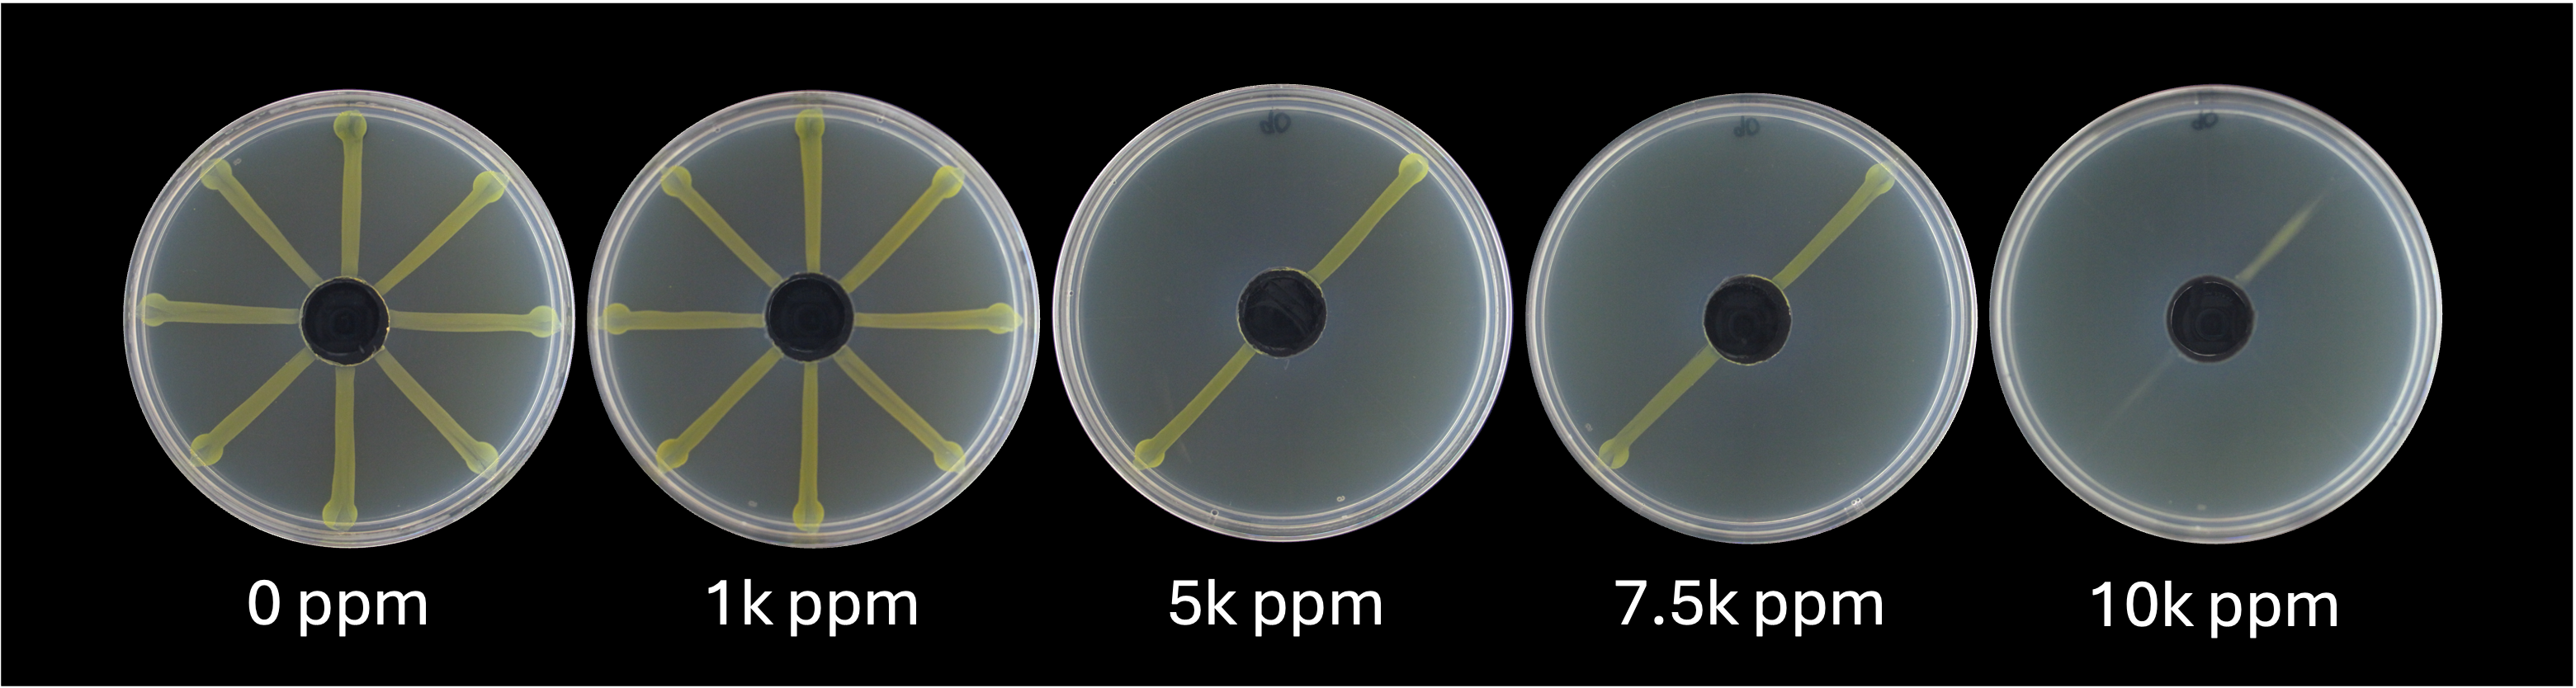
\includegraphics[width=0.8\linewidth,height=1\textheight]{Figures/Cu_Plates} 

}

\caption{\textit{In vitro} copper sensitivity. Pictured are strains $\text{XAJ}1606$, $\text{XAJ}355$, $\text{XAP}880$, and $\text{XAP}883$.}\label{fig:CuPlates}
\end{figure}

\begin{figure}

{\centering 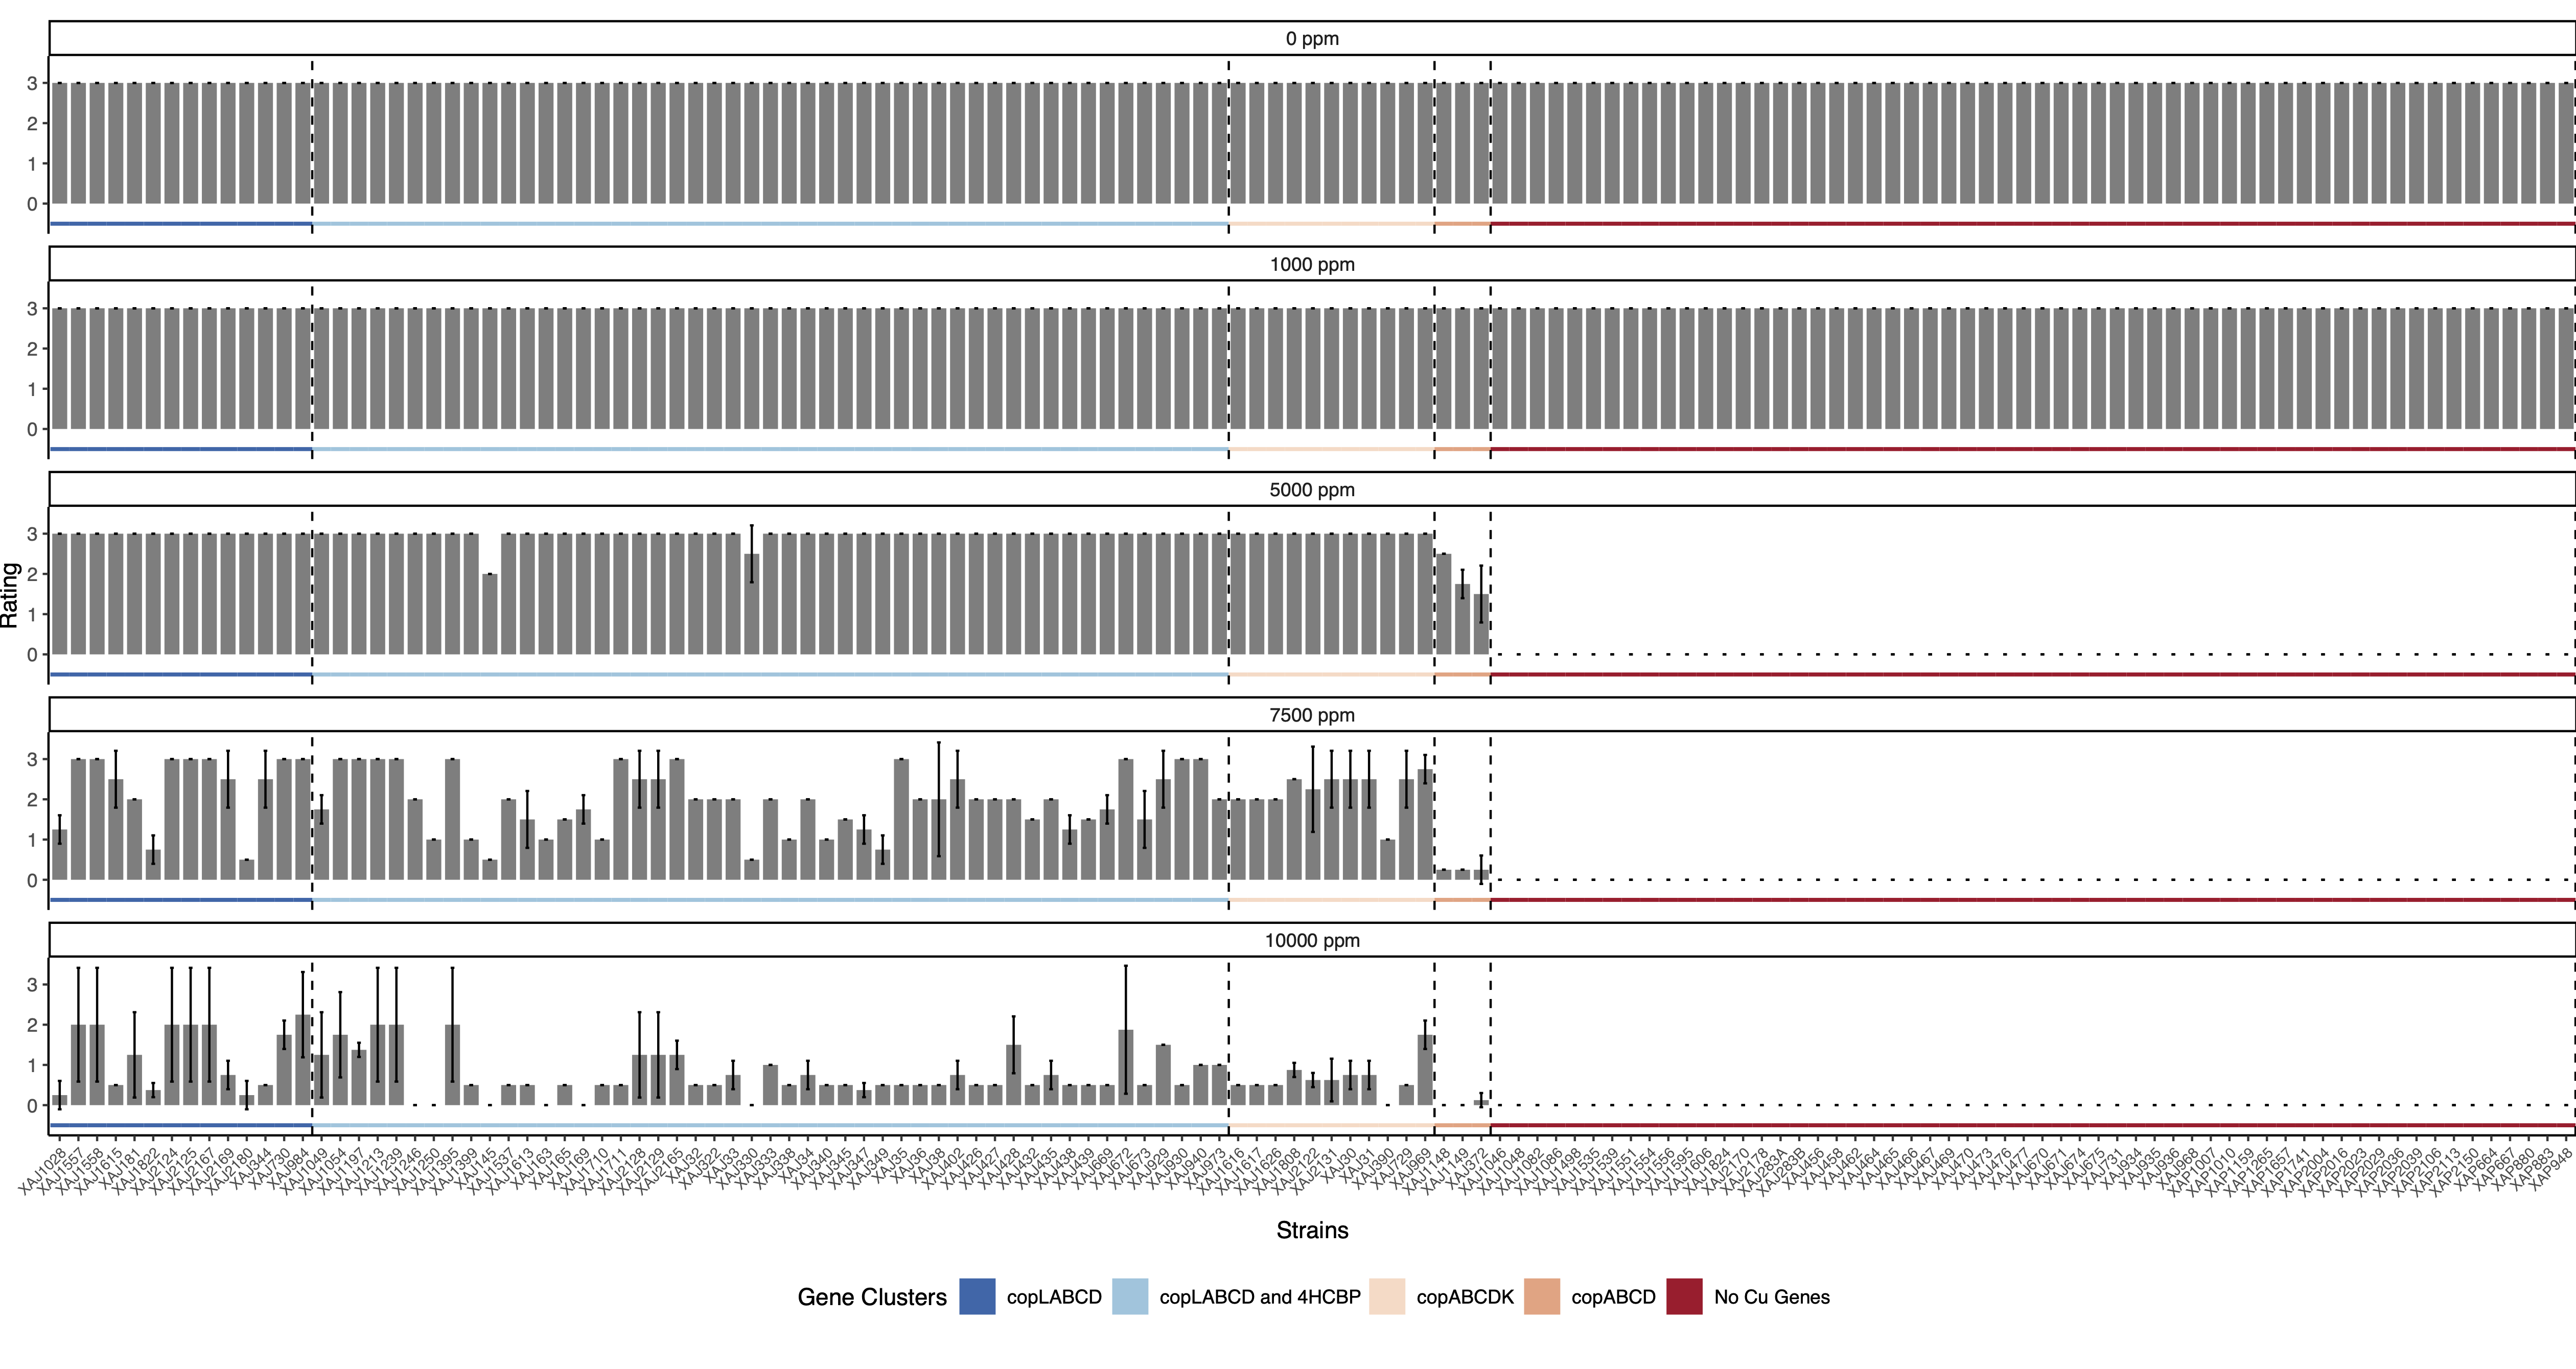
\includegraphics[width=1\linewidth,height=1\textheight]{Figures/Xaj_Xap_Cu_Assay_Barplot} 

}

\caption{\textit{In vitro} copper sensitivity results for all strains ($\text{n}=135$).}\label{fig:CuAll}
\end{figure}

\begin{figure}

{\centering 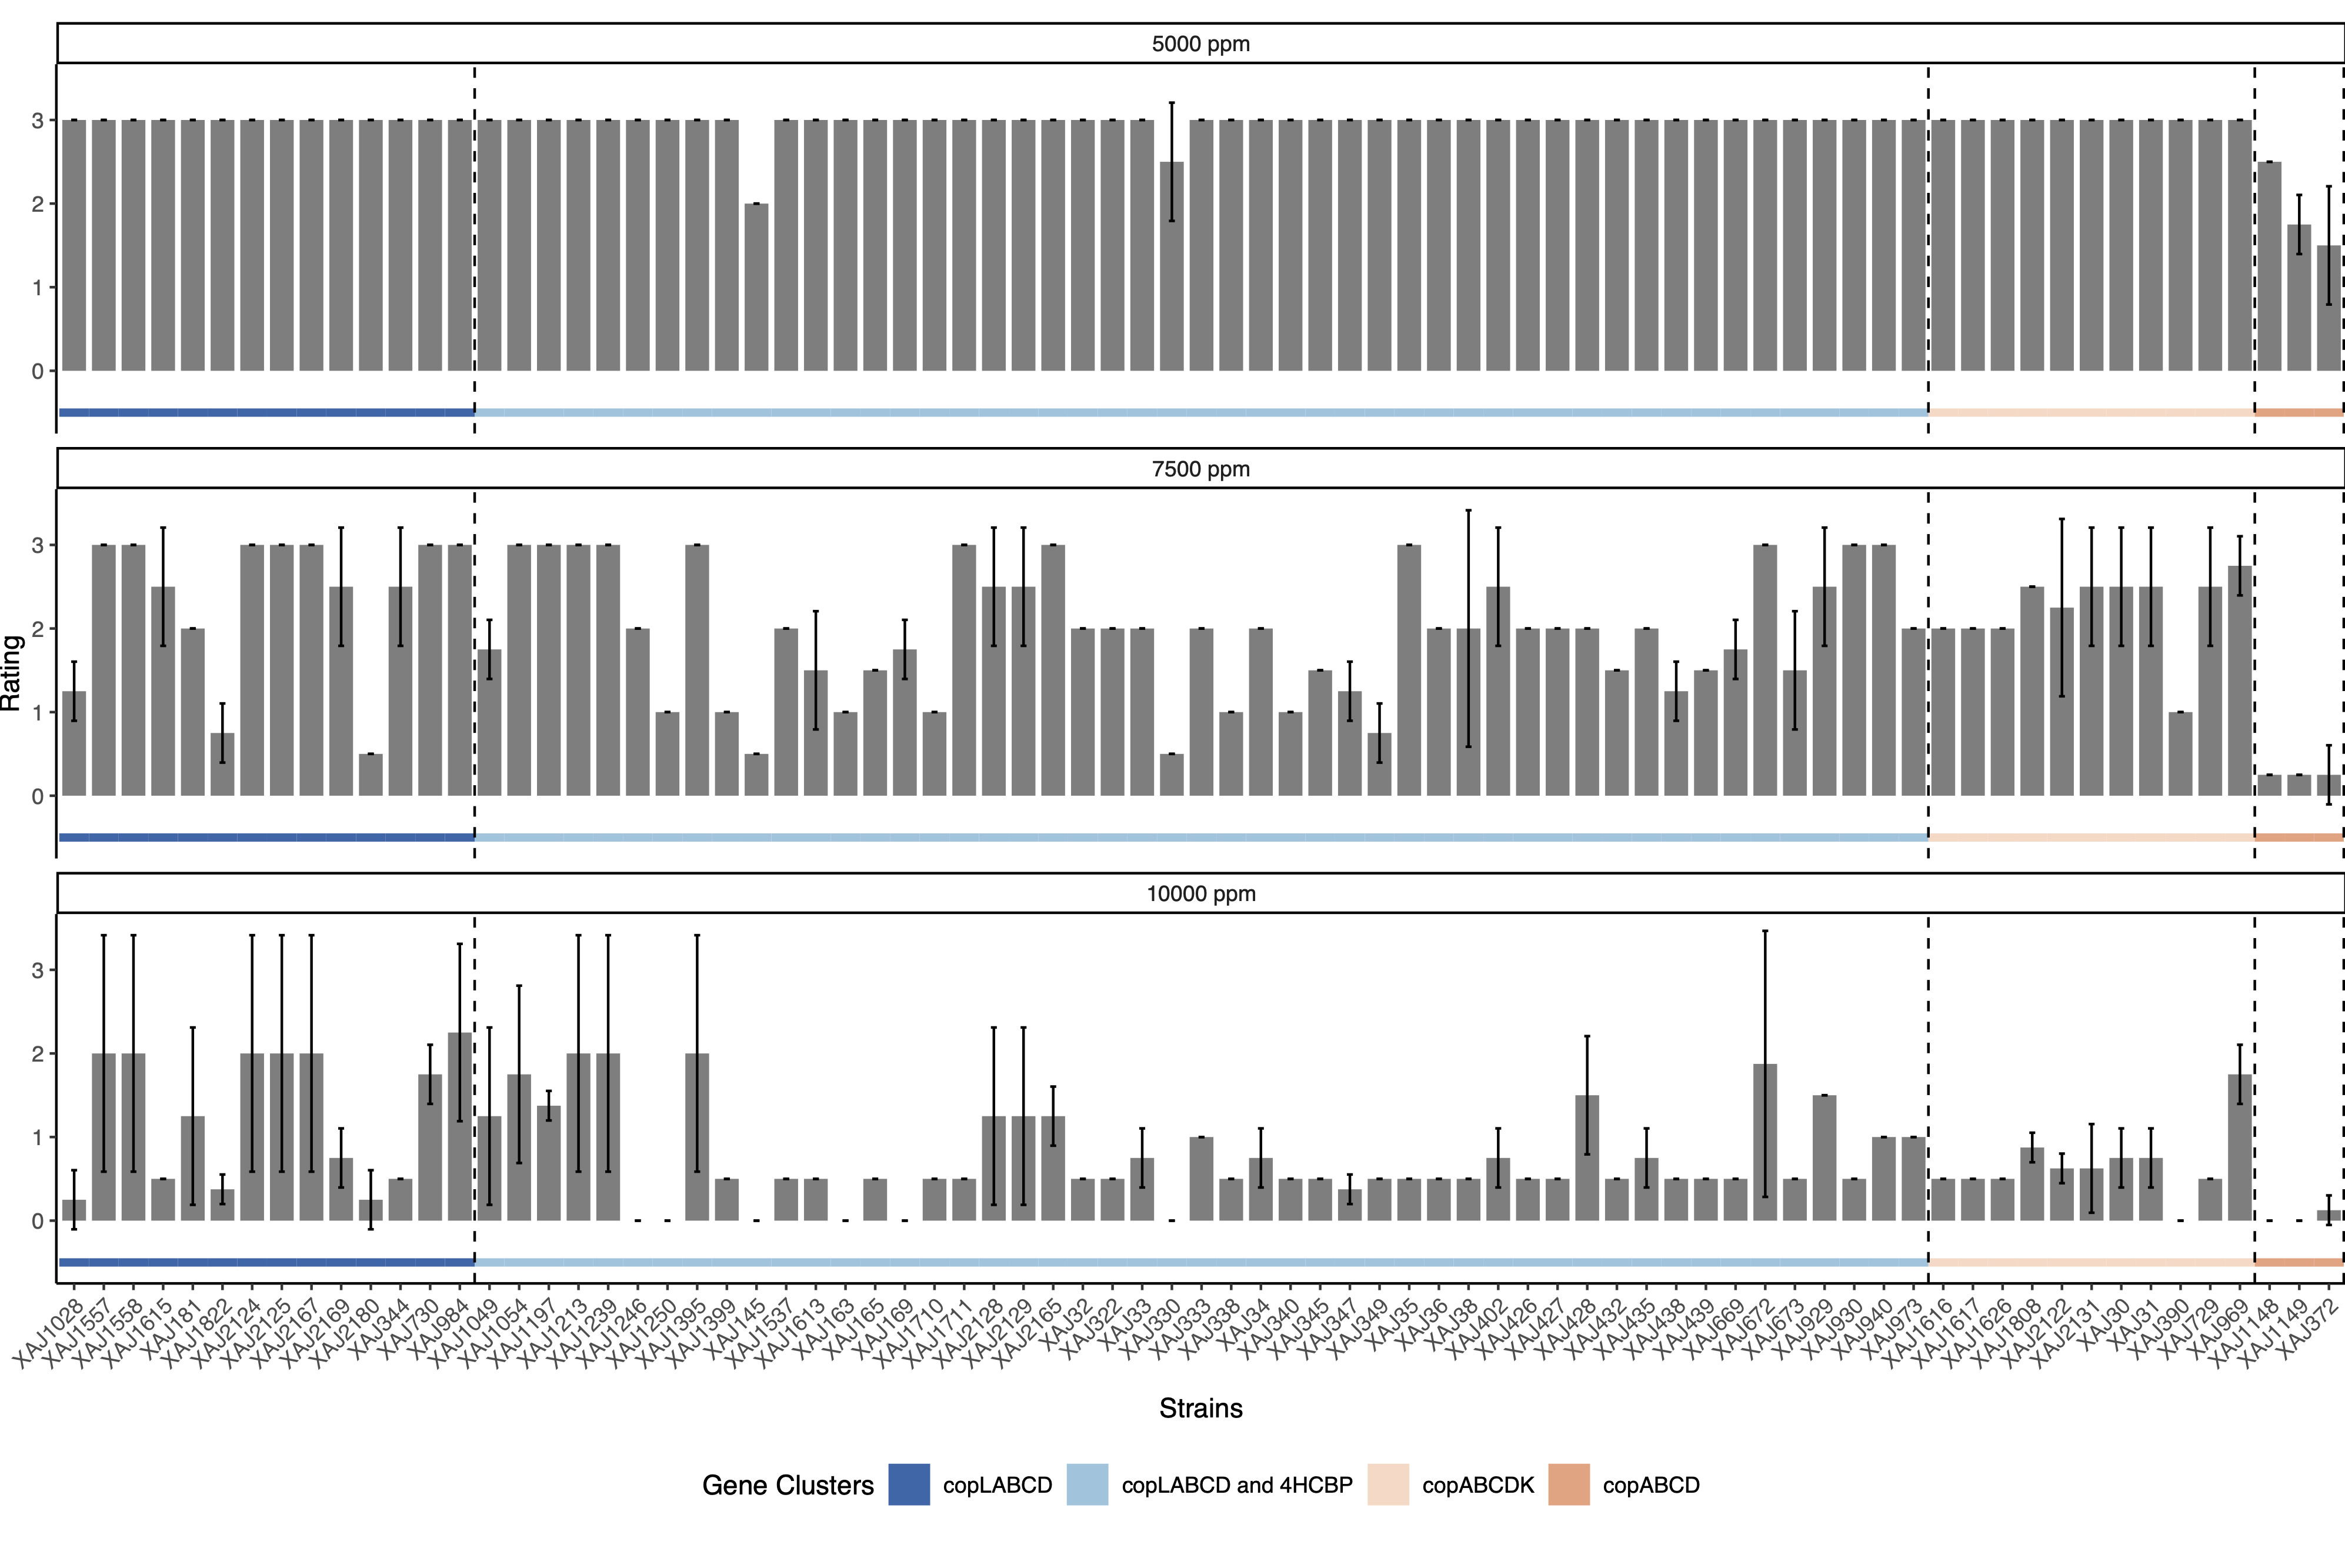
\includegraphics[width=1\linewidth,height=1\textheight]{Figures/Xaj_Xap_Cu_Assay_Barplot_CuResistantOnly} 

}

\caption{\textit{In vitro} copper sensitivity of the copper-resistant strains ($\text{n}=77$).}\label{fig:CuRes}
\end{figure}

\section{Pangenome Analyses (NEED TO FINISH)}\label{pangenome-analyses-need-to-finish}

The pangenome analysis using \texttt{PPanGGoLiN} was successful. I will describe the results based on the respective runs: CA\_XAJ\_115 (n=115) and CA\_XAJ\_115\_XAP (n=135), with more emphasis on the CA\_XAJ\_115 since that will be the data we use for the manuscript. The gene presence/absence data was used to identify genes related to copper resistance as well as Type III effectors. The pangenome graph was used to visualize the various partitions (`persistent', `shell', and `cloud').

\subsection{\texorpdfstring{CA \emph{Xaj} (n=115)}{CA Xaj (n=115)}}\label{ca-xaj-n115}

The presence absence matrix file this data was acquired from is \texttt{matrix\_Xaj\_115.xlsx}.

\subsubsection{Pangenome Partitions}\label{pangenome-partitions}

A pangenome graph was generated with \texttt{Gephi} using the \texttt{pangenomeGraph.gexf} as the input file. Nodes represent gene families (clusters of homologous genes across the input genomes). Edges connect gene families that are genomic neighbors (i.e., their sequences are adjacent in at least one genome). The graph is partitioned into categories---persistent, shell, and cloud---based on how frequently gene families appear across genomes and their neighborhood relationships. This structure resembles a ``subway map'' of genomic diversity, allowing you to visualize the core and variable components of a species' pangenome. The `persistent,' `shell,' and `cloud' genomes constitute 69.95\%, 19.14\%, and 10.91\% of the pangenome, respectively (\ref{fig:PGgraph}).

\begin{figure}

{\centering 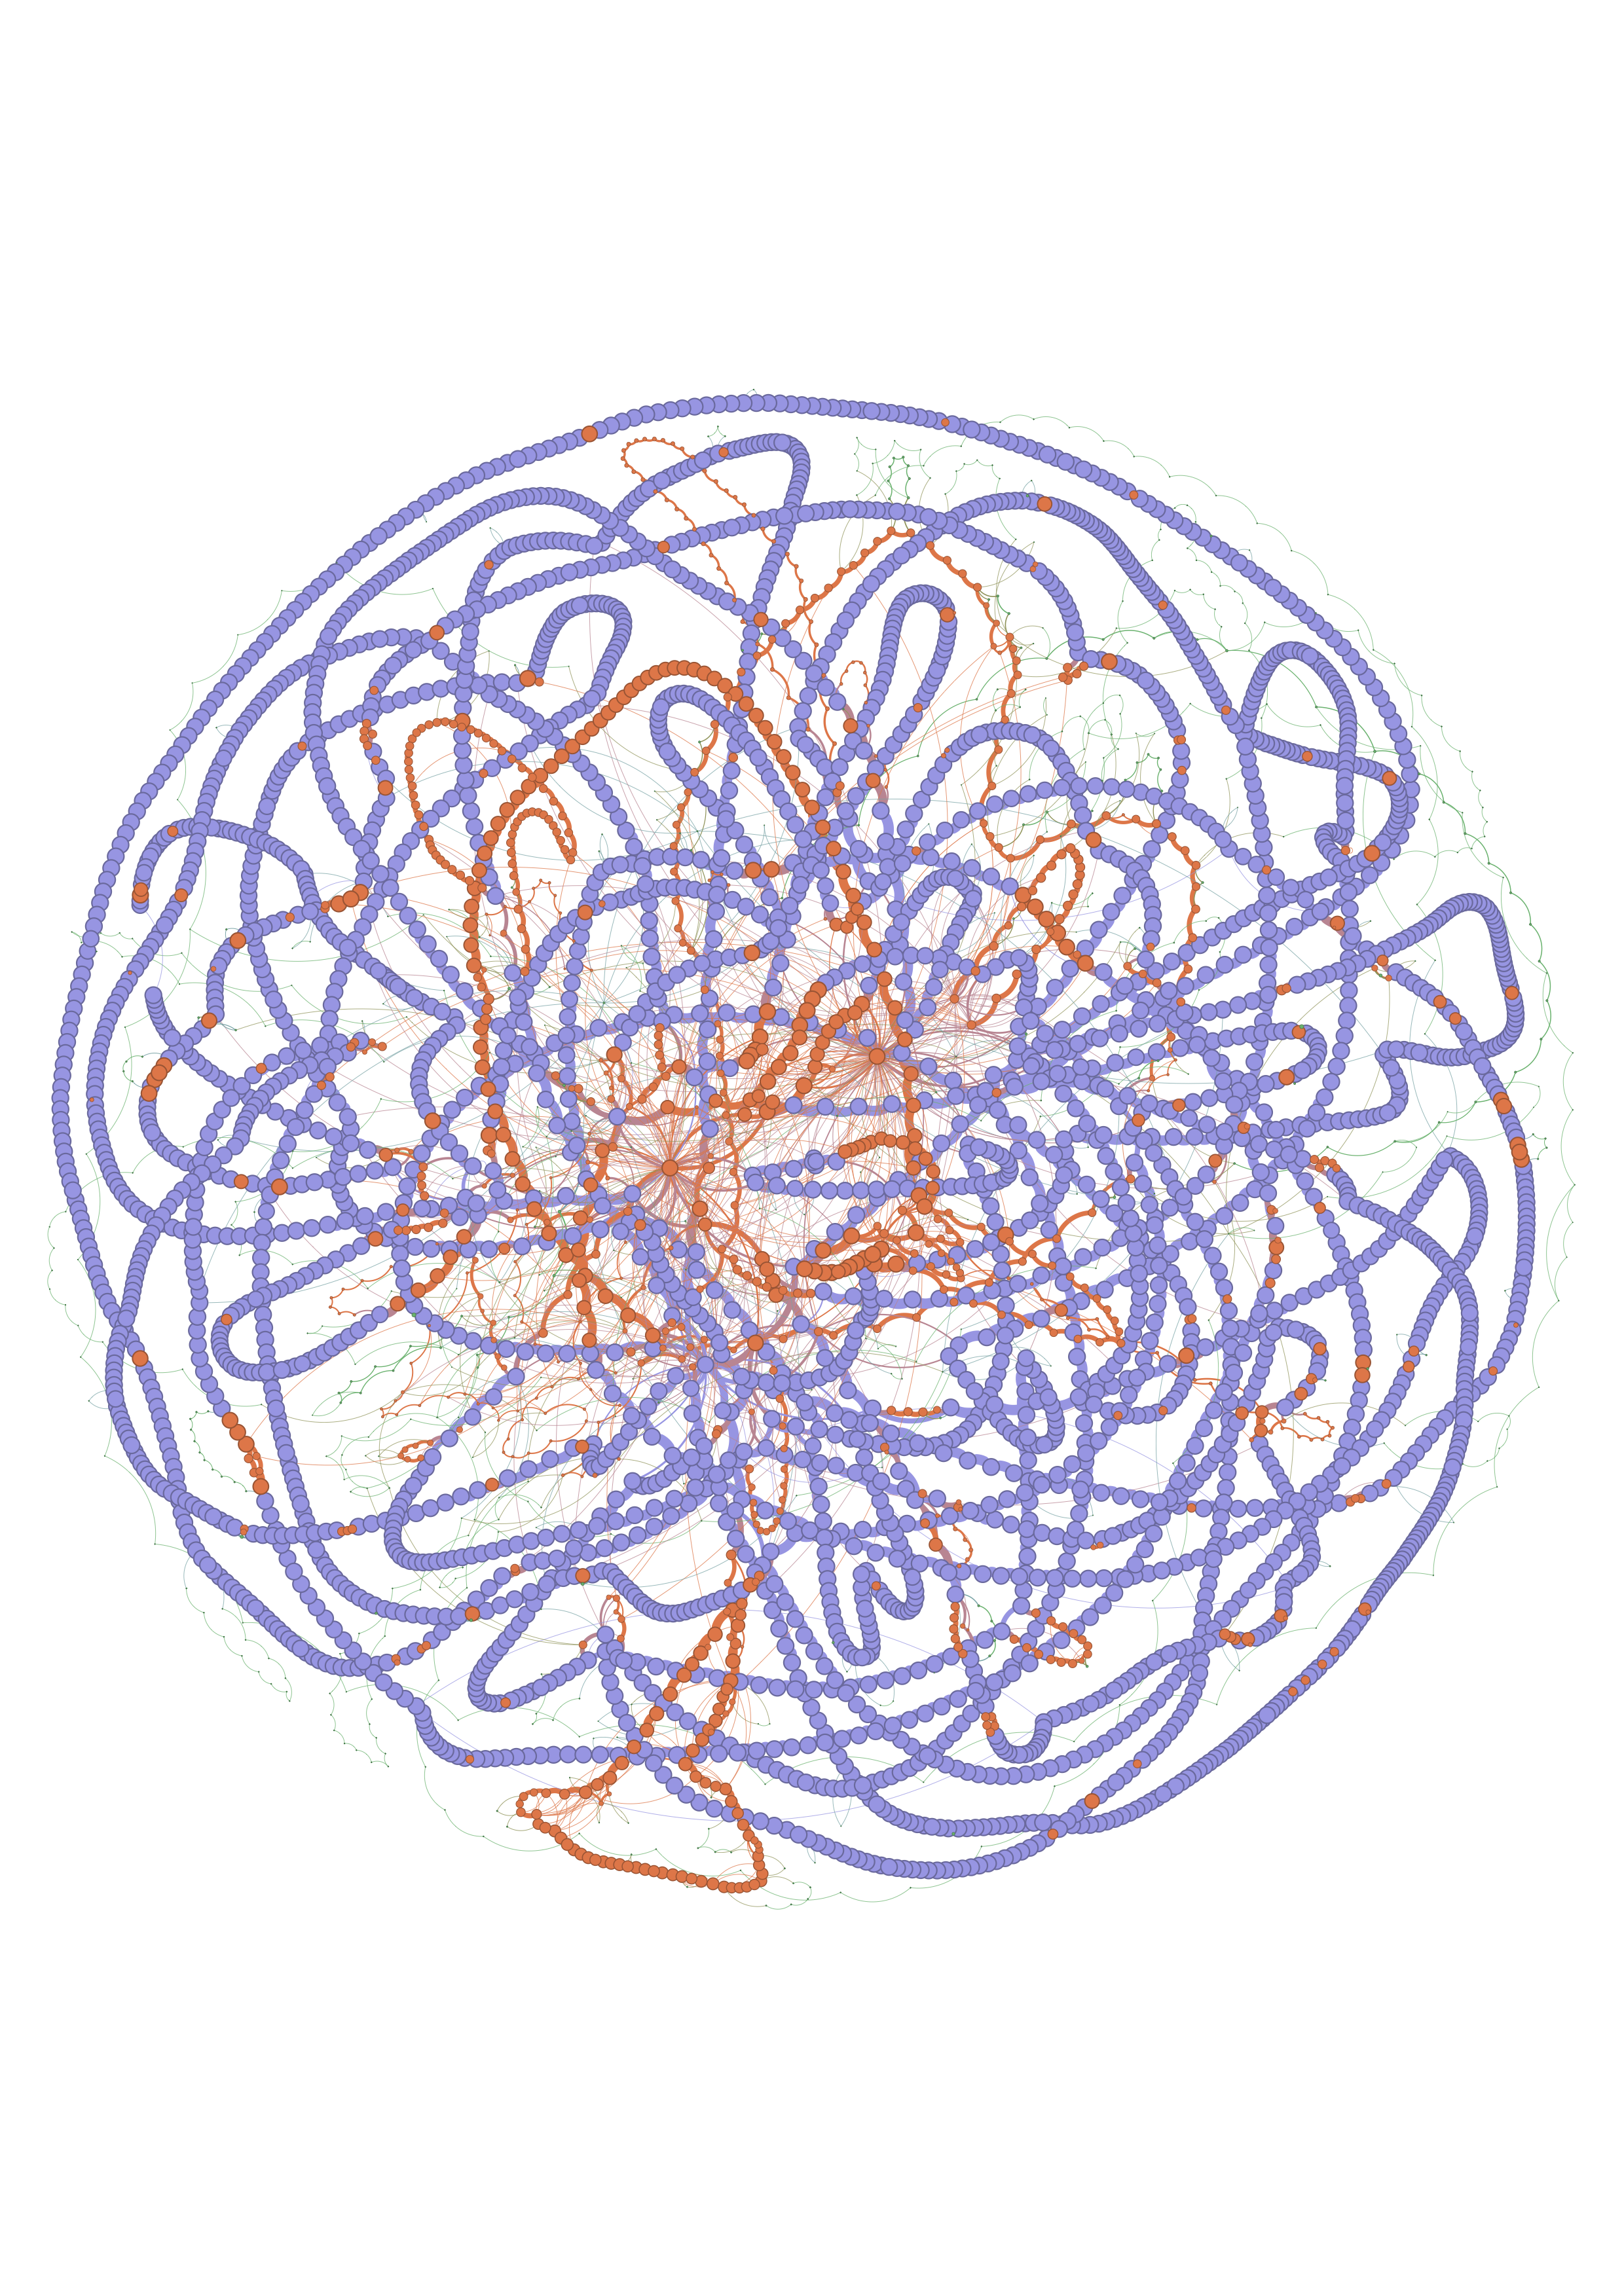
\includegraphics[width=1\linewidth,height=1\textheight]{Figures/CA_XAJ_115_Pangenome_Graph} 

}

\caption{Pangenome graph of the 115 CA \textit{Xaj} strains. 'Persistent': purple; 'shell': orange; 'cloud': green.}\label{fig:PGgraph}
\end{figure}

\subsubsection{Copper Resistance-Related Genes}\label{copper-resistance-related-genes}

Various copper resistance-related genes have been characterized in \emph{Xanthomonas} and in \emph{Xaj}. These genes include: \emph{copL}, \emph{copA}, \emph{copB}, \emph{copC}, \emph{copD}, and \emph{copK} (\citet{lee1994}; cesbron2015; \citet{marin2019}; \citet{assis2021}). The \emph{copA} and \emph{copC} genes encode periplasmic copper-binding proteins, conferring partial copper resistance in \emph{P. syringae} (\citet{marin2019}). In \emph{X. citri}, \citet{richard2017} reported plasmid-bore copper resistance genes termed \emph{copABCD}, however in \emph{Xaj} these genes are found on the chromosome (\citet{lee1994}; \citet{giovanardi2016}; \citet{assis2021}). In both copper-sensitive (CuS) and copper-resistant (CuR) \emph{Xanthomonas} strains, the chromosomal genes \emph{cohL}, \emph{cohA}, and \emph{cohB}, involved in copper homeostasis, exhibit homology to cop resistance genes located on plasmids (\citet{behlau2011}; \citet{behlau2016}).

The \texttt{PPanGGoLiN} analysis successfully identified copper resistance-related genes as well as the copper homeostatsis genes. The genes associated with copper resistance are \emph{copL} family metal-binding regulatory protein, copper resistance system multicopper oxidase ( \emph{copA} ), copper resistance protein B ( \emph{copB} ), copper homeostasis periplasmic binding protein \emph{copC}, copper homeostasis membrane protein \emph{copD}, and \emph{copK} family periplasmic copper-binding protein. Each of these six genes are present in the `shell' or `cloud' partitions and while the respective \emph{copL}, \emph{copA}, \emph{copB} homeostasis genes are present in the `persistent' genome and found in all 115 strains (\ref{tab:CAxajCuGenes}).

A total of 77 strains were found to encode copper resistance genes ( \emph{copA}, \emph{copB}, \emph{copC}, \emph{copD}, and \emph{copK}) in various combinations and copy number. These same 77 strains were also characterized as CuR based on the \emph{in vitro} sensitivity assay.

\begin{longtable}[]{@{}
  >{\centering\arraybackslash}p{(\columnwidth - 10\tabcolsep) * \real{0.1667}}
  >{\centering\arraybackslash}p{(\columnwidth - 10\tabcolsep) * \real{0.1667}}
  >{\centering\arraybackslash}p{(\columnwidth - 10\tabcolsep) * \real{0.1667}}
  >{\centering\arraybackslash}p{(\columnwidth - 10\tabcolsep) * \real{0.1667}}
  >{\centering\arraybackslash}p{(\columnwidth - 10\tabcolsep) * \real{0.1667}}
  >{\centering\arraybackslash}p{(\columnwidth - 10\tabcolsep) * \real{0.1667}}@{}}
\caption{\label{tab:CAxajCuGenes} Genes associated with copper resistance and homeostasis. The annotations have been shortened, see \texttt{matrix\_Xaj\_115.xlsx} tab \texttt{Copper-resistance} for the full annotations.}\tabularnewline
\toprule\noalign{}
\begin{minipage}[b]{\linewidth}\centering
\textbf{Gene (PPanGGoLiN ID)}
\end{minipage} & \begin{minipage}[b]{\linewidth}\centering
\textbf{Partition}
\end{minipage} & \begin{minipage}[b]{\linewidth}\centering
\textbf{Annotation}
\end{minipage} & \begin{minipage}[b]{\linewidth}\centering
\textbf{No.~strains}
\end{minipage} & \begin{minipage}[b]{\linewidth}\centering
\textbf{No.~seqs}
\end{minipage} & \begin{minipage}[b]{\linewidth}\centering
\textbf{Avg seq per strain}
\end{minipage} \\
\midrule\noalign{}
\endfirsthead
\toprule\noalign{}
\begin{minipage}[b]{\linewidth}\centering
\textbf{Gene (PPanGGoLiN ID)}
\end{minipage} & \begin{minipage}[b]{\linewidth}\centering
\textbf{Partition}
\end{minipage} & \begin{minipage}[b]{\linewidth}\centering
\textbf{Annotation}
\end{minipage} & \begin{minipage}[b]{\linewidth}\centering
\textbf{No.~strains}
\end{minipage} & \begin{minipage}[b]{\linewidth}\centering
\textbf{No.~seqs}
\end{minipage} & \begin{minipage}[b]{\linewidth}\centering
\textbf{Avg seq per strain}
\end{minipage} \\
\midrule\noalign{}
\endhead
\bottomrule\noalign{}
\endlastfoot
ACETXQ\_000680 & cloud & \emph{copA} & 3 & 3 & 1 \\
ACETXQ\_000681 & cloud & \emph{copB} & 3 & 3 & 1 \\
ACETXQ\_000677 & cloud & \emph{copC} & 3 & 3 & 1 \\
ACETXQ\_000676 & cloud & \emph{copD} & 3 & 3 & 1 \\
ACETZU\_002144 & cloud & \emph{copA} & 11 & 11 & 1 \\
ACETY7\_002282 & cloud & \emph{copB} & 11 & 11 & 1 \\
ACETY7\_002278 & cloud & \emph{copC} & 11 & 11 & 1 \\
ACETY7\_002277 & cloud & \emph{copD} & 11 & 11 & 1 \\
ACETY7\_002276 & cloud & \emph{copK} & 11 & 11 & 1 \\
ACETYR\_002169 & shell & \emph{copL} & 59 & 107 & 1.81 \\
ACETYY\_002111 & shell & \emph{copL} & 63 & 111 & 1.76 \\
ACETZG\_002299 & shell & \emph{copA} & 63 & 111 & 1.76 \\
ACETZG\_002300 & shell & \emph{copB} & 63 & 111 & 1.76 \\
ACETZG\_002301 & shell & \emph{copC} & 63 & 111 & 1.76 \\
ACETZG\_002302 & shell & \emph{copD} & 63 & 111 & 1.76 \\
ACETZG\_003906 & persistent & \emph{copL} & 115 & 115 & 1 \\
ACET0S\_003856 & persistent & \emph{copA} & 115 & 115 & 1 \\
ACETZG\_003908 & persistent & \emph{copB} & 115 & 115 & 1 \\
\end{longtable}

\subsubsection{Type III Effectors}\label{type-iii-effectors}

The presence/absence matrix (\texttt{matrix\_Xaj\_115.xlsx}) was used to identify type III effectors (T3Es) by searching for the term ``tpye III secretion system effector'' in the `Annotations' column. I was able to identify 18 effectors using this method. After cross-referencing the tBLASTn \& BLASTp results, I was able to identify 4 more that did not have ``type III secretion system effector'' in the annotation but were determined to be T3Es by Method 3 (\ref{T3EMeth}).

Only two T3Es were identified in the presence/absence matrix, \emph{XopR} and \emph{XopAH}, that were not captured by Method 3 (\textbf{LINK METHOD 3 RESULTS TABLE}).

\begin{itemize}
\item
  The XAJ283A \emph{XopAH} gene (ACET0C\_003701) was present in the raw \texttt{BLASTp} and \texttt{tBLASTn} outputs but exhibited \textasciitilde28\% identity with E-values of 5.11e-33 and 1.53e-36 to WP\_011037263.1 (\emph{XopAH}), respectively. I performed a web-based BLASTp with XAJ283A's \emph{XopAH} gene ACET0C\_003701 it yielded \textgreater99\% ID to X. arboricola ``XopAH/AvrB family type III secretion system effector'' (WP\_372159172.1, WP\_080591327.1, and WP\_258077835.1) and to Xaj ``type III effector protein AvrB3'' (AKU50911.1). The reason that this gene was not captured in the BLAST analyses is likely because the reference \emph{XopAH} \href{https://www.ncbi.nlm.nih.gov/protein/WP_011037263.1}{WP\_011037263.1} is a \emph{X. campestris} protein and exhibited too much sequence variation to the query \emph{Xaj} sequences.
\item
  The XAJ283A \emph{XopR} gene (ACET0C\_000329) was present in the raw \texttt{BLASTp} and \texttt{tBLASTn} outputs but exhibited \textasciitilde37\% and \textasciitilde44\% identity with E-values of 2.12e-60 and 4.89e-36 to WP\_011260681.1 (\emph{XopR}), respectively. I performed a web-based BLASTp with XAJ283A's \emph{XopR} gene ACET0C\_000329 it yielded 100\% and 99.76 \% idenetity to \emph{X. arboricola} ``type III secretion system effector protein \emph{XopR}'' (WP\_104538897.1) and to the \emph{X. arboricola} pv. \emph{corylina} ``type III secretion system effector protein \emph{XopR}'' (WIX26666.1), respectively. The reason this gene was not captured in the BLAST analyses is likely because the reference \emph{XopR} sequence (\href{https://www.ncbi.nlm.nih.gov/protein/WP_011260681.1}{WP\_011260681.1}) is a MULTISPECIES \emph{Xanthomonas} \emph{XopR} sequence and exhibited too much sequence variation to the query \emph{Xaj} sequences.
\end{itemize}

The respective protein sequences for XopR and XopAH in strain Xaj283A were subjected to a web-based BLASTp search and the results yielded (\ref{tab:PangT3E}).

\begin{longtable}[]{@{}
  >{\centering\arraybackslash}p{(\columnwidth - 14\tabcolsep) * \real{0.1250}}
  >{\centering\arraybackslash}p{(\columnwidth - 14\tabcolsep) * \real{0.1250}}
  >{\centering\arraybackslash}p{(\columnwidth - 14\tabcolsep) * \real{0.1250}}
  >{\centering\arraybackslash}p{(\columnwidth - 14\tabcolsep) * \real{0.1250}}
  >{\centering\arraybackslash}p{(\columnwidth - 14\tabcolsep) * \real{0.1250}}
  >{\centering\arraybackslash}p{(\columnwidth - 14\tabcolsep) * \real{0.1250}}
  >{\centering\arraybackslash}p{(\columnwidth - 14\tabcolsep) * \real{0.1250}}
  >{\centering\arraybackslash}p{(\columnwidth - 14\tabcolsep) * \real{0.1250}}@{}}
\caption{\label{tab:PangT3E} Type III effectors identified from the PPanGGoLiN presence/absence matrix (\texttt{matrix\_Xaj\_115.xlsx}).}\tabularnewline
\toprule\noalign{}
\begin{minipage}[b]{\linewidth}\centering
\textbf{Gene (PPanGGoLiN ID)}
\end{minipage} & \begin{minipage}[b]{\linewidth}\centering
\textbf{Partition}
\end{minipage} & \begin{minipage}[b]{\linewidth}\centering
\textbf{T3E}
\end{minipage} & \begin{minipage}[b]{\linewidth}\centering
\textbf{No.~strains}
\end{minipage} & \begin{minipage}[b]{\linewidth}\centering
\textbf{No.~sequences}
\end{minipage} & \begin{minipage}[b]{\linewidth}\centering
\textbf{Avg sequences per strain}
\end{minipage} & \begin{minipage}[b]{\linewidth}\centering
\textbf{Captured by Method 3?}
\end{minipage} & \begin{minipage}[b]{\linewidth}\centering
\textbf{Type}
\end{minipage} \\
\midrule\noalign{}
\endfirsthead
\toprule\noalign{}
\begin{minipage}[b]{\linewidth}\centering
\textbf{Gene (PPanGGoLiN ID)}
\end{minipage} & \begin{minipage}[b]{\linewidth}\centering
\textbf{Partition}
\end{minipage} & \begin{minipage}[b]{\linewidth}\centering
\textbf{T3E}
\end{minipage} & \begin{minipage}[b]{\linewidth}\centering
\textbf{No.~strains}
\end{minipage} & \begin{minipage}[b]{\linewidth}\centering
\textbf{No.~sequences}
\end{minipage} & \begin{minipage}[b]{\linewidth}\centering
\textbf{Avg sequences per strain}
\end{minipage} & \begin{minipage}[b]{\linewidth}\centering
\textbf{Captured by Method 3?}
\end{minipage} & \begin{minipage}[b]{\linewidth}\centering
\textbf{Type}
\end{minipage} \\
\midrule\noalign{}
\endhead
\bottomrule\noalign{}
\endlastfoot
ACETYW\_002316 & cloud & \emph{AvrBs1} & 2 & 2 & 1 & Yes & Variable \\
ACETYW\_002318 & cloud & \emph{XopH1} & 2 & 2 & 1 & Yes & Variable \\
ACETZ0\_003513 & cloud & \emph{XopG2} & 14 & 14 & 1 & Yes & Variable \\
ACETZG\_004545 & persistent & \emph{AvrBs2} & 115 & 115 & 1 & Yes & Core \\
ACETZV\_000338 & persistent & \emph{XopR} & 115 & 115 & 1 & No & Core \\
ACETZG\_001290 & persistent & \emph{XopAV1} & 115 & 115 & 1 & Yes & Core \\
ACETZG\_001291 & persistent & \emph{XopAV2} & 115 & 115 & 1 & Yes & Core \\
ACETZG\_000577 & persistent & \emph{XopF1} & 115 & 115 & 1 & Yes & Core \\
ACETZG\_003328 & persistent & \emph{XopK} & 115 & 115 & 1 & Yes & Core \\
ACETZG\_003062 & persistent & \emph{XopK} & 115 & 115 & 1 & Yes & Core \\
ACETZG\_001289 & persistent & \emph{XopQ} & 115 & 115 & 1 & Yes & Core \\
ACETZG\_003209 & persistent & \emph{XopAW} & 112 & 112 & 1 & Yes & Variable \\
ACETZG\_000745 & persistent & \emph{XopV} & 115 & 115 & 1 & Yes & Core \\
ACETZG\_000656 & persistent & \emph{XopX} & 115 & 115 & 1 & Yes & Core \\
ACETZG\_002419 & persistent & \emph{XopZ} & 115 & 115 & 1 & Yes & Core \\
ACETZG\_003349 & persistent & \emph{XopL} & 115 & 115 & 1 & Yes & Core \\
ACETZG\_000602 & persistent & \emph{XopM} & 115 & 115 & 1 & Yes & Core \\
ACETZG\_001505 & persistent & \emph{XopAZ} & 115 & 115 & 1 & Yes & Core \\
ACETZG\_001286 & shell & \emph{XopG3} & 110 & 110 & 1 & Yes & Variable \\
ACETY6\_003877 & shell & \emph{XopAI} & 48 & 48 & 1 & Yes & Variable \\
ACETYR\_003597 & shell & \emph{XopAH} & 78 & 79 & 1.01 & No & Variable \\
ACETZG\_002185 & shell & \emph{XopE4} & 53 & 53 & 1 & Yes & Variable \\
\end{longtable}

\subsubsection{\texorpdfstring{Modules, Spots, and RGPs (\textbf{LEFT OFF HERE!!!})}{Modules, Spots, and RGPs (LEFT OFF HERE!!!)}}\label{modules-spots-and-rgps-left-off-here}

\textbf{Modules}

\begin{itemize}
\item
  Definition: Modules in PPanGGOLiN are conserved groups of genes, typically from the variable (shell and cloud) genome, that tend to co-occur and are co-localized across multiple genomes in the pangenome. These are often hypothesized to represent functional units that are gained or lost together.
\item
  How They're Generated: Modules are predicted using the panModule method, which analyzes patterns of gene co-occurrence and genomic neighborhood within RGPs. The process involves identifying clusters of genes that consistently appear together in the variable regions of the pangenome.
\end{itemize}

\textbf{Spots}

\begin{itemize}
\item
  Definition: Spots, or Spots of Insertion, are groups of RGPs from different genomes that share conserved flanking persistent genes, indicating a common insertion site in the pangenome. They represent hotspots of genomic variability.
\item
  How They're Generated: After RGPs are identified, the spot command groups them into Spots based on shared genomic context (persistent gene borders). This clustering reflects where RGPs tend to integrate across the pangenome.
\end{itemize}

\textbf{RGPs (Regions of Genomic Plasticity)}

\begin{itemize}
\item
  Definition: RGPs are genomic regions in individual genomes that consist of genes from the shell and cloud partitions (i.e., non-persistent genes). These regions are typically associated with horizontal gene transfer (HGT) and often correspond to Genomic Islands (GIs).
\item
  How They're Generated: The panRGP method identifies RGPs by scanning each genome and detecting clusters of consecutive shell or cloud genes, using a score-based algorithm to define boundaries. Persistent genes flanking these regions help delineate them.
\end{itemize}

\textbf{Interconnection}

\begin{itemize}
\item
  Modules, RGPs, and Spots are interconnected: Modules are often subsets of genes within RGPs, and Spots group RGPs across genomes. The --spot\_modules option ties these together by associating Modules with specific Spots and RGPs, enabling a deeper understanding of how conserved gene clusters relate to variable genomic regions.
\item
  Purpose: Together, these features allow PPanGGOLiN to depict microbial diversity by partitioning the pangenome into persistent, shell, and cloud components, then analyzing the variable regions for patterns of conservation and plasticity.
\end{itemize}

\section{Phylogenetic Analyses (NEED TO FINISH)}\label{phylogenetic-analyses-need-to-finish}

\begin{figure}

{\centering 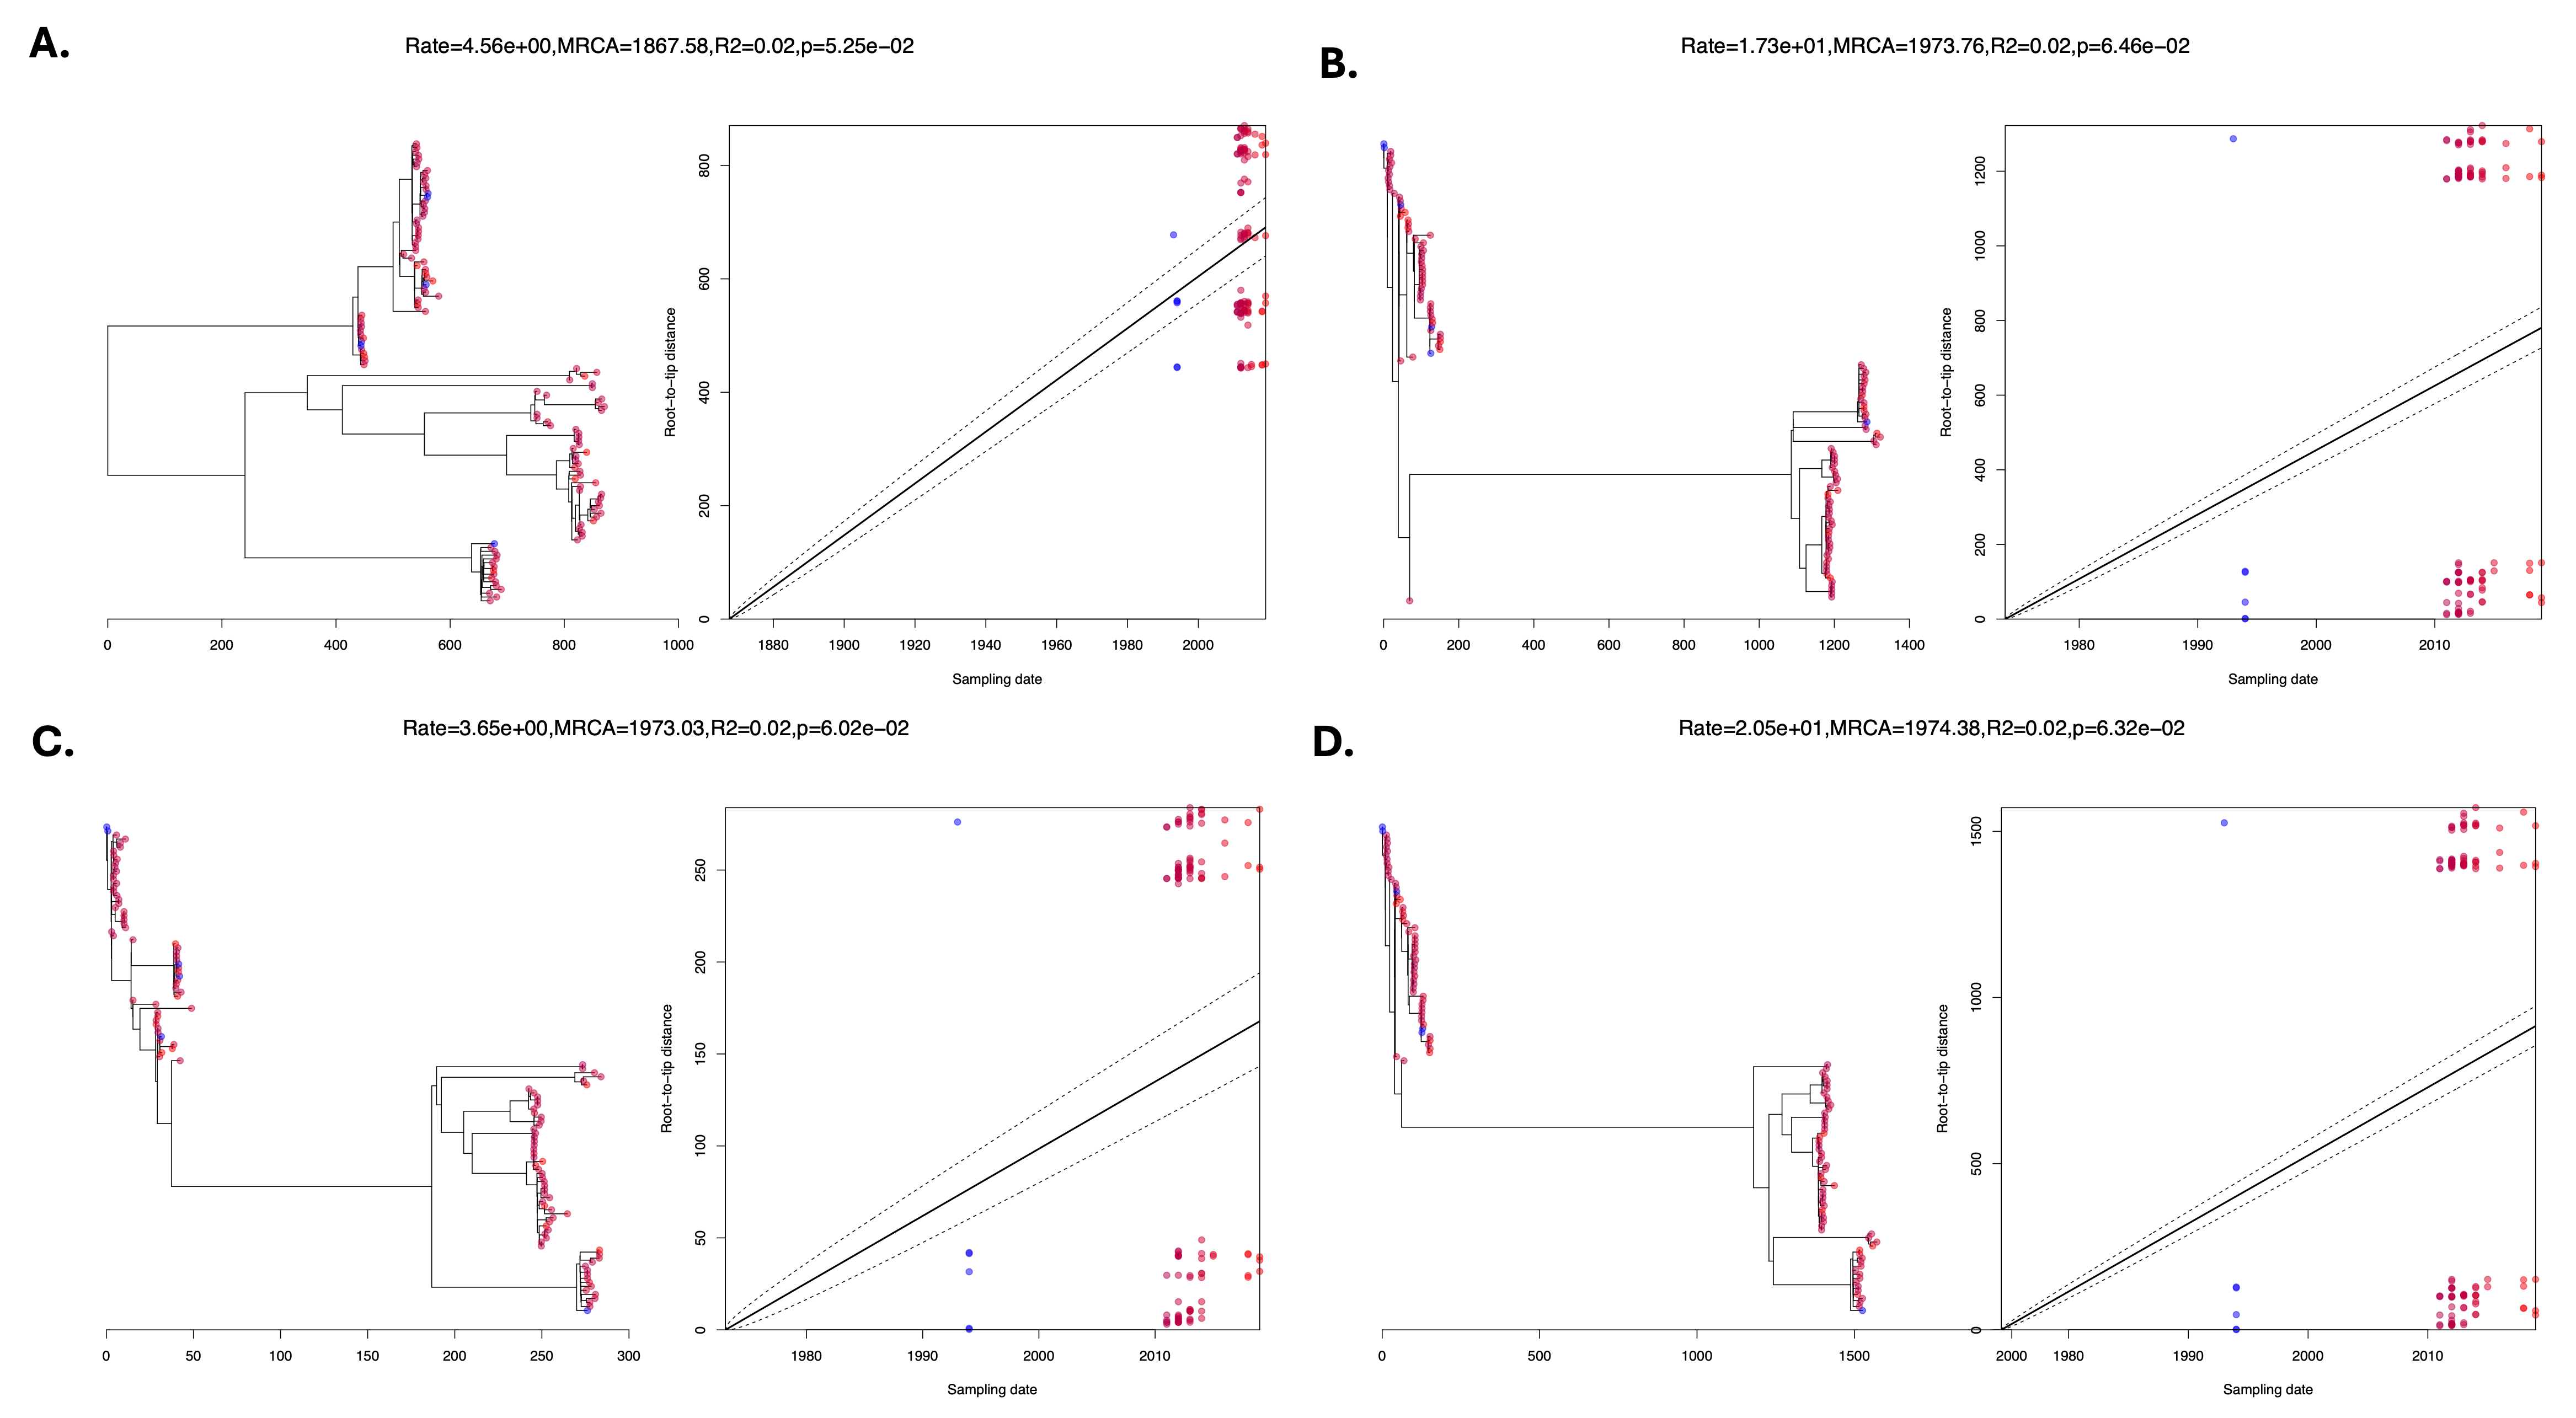
\includegraphics[width=1\linewidth,height=1\textheight]{Figures/CA_XAJ_Root2tip} 

}

\caption{Root-to-tip regression analysis on CA\_XAJ using BactDating. \textbf{A.} ClonalFrameML. \textbf{B.} Gubbins. \textbf{C.} ClonalFrameML and IQtree. \textbf{D.} ClonalFrameML and Gubbins}\label{fig:CAXAJR2T}
\end{figure}

\begin{figure}

{\centering 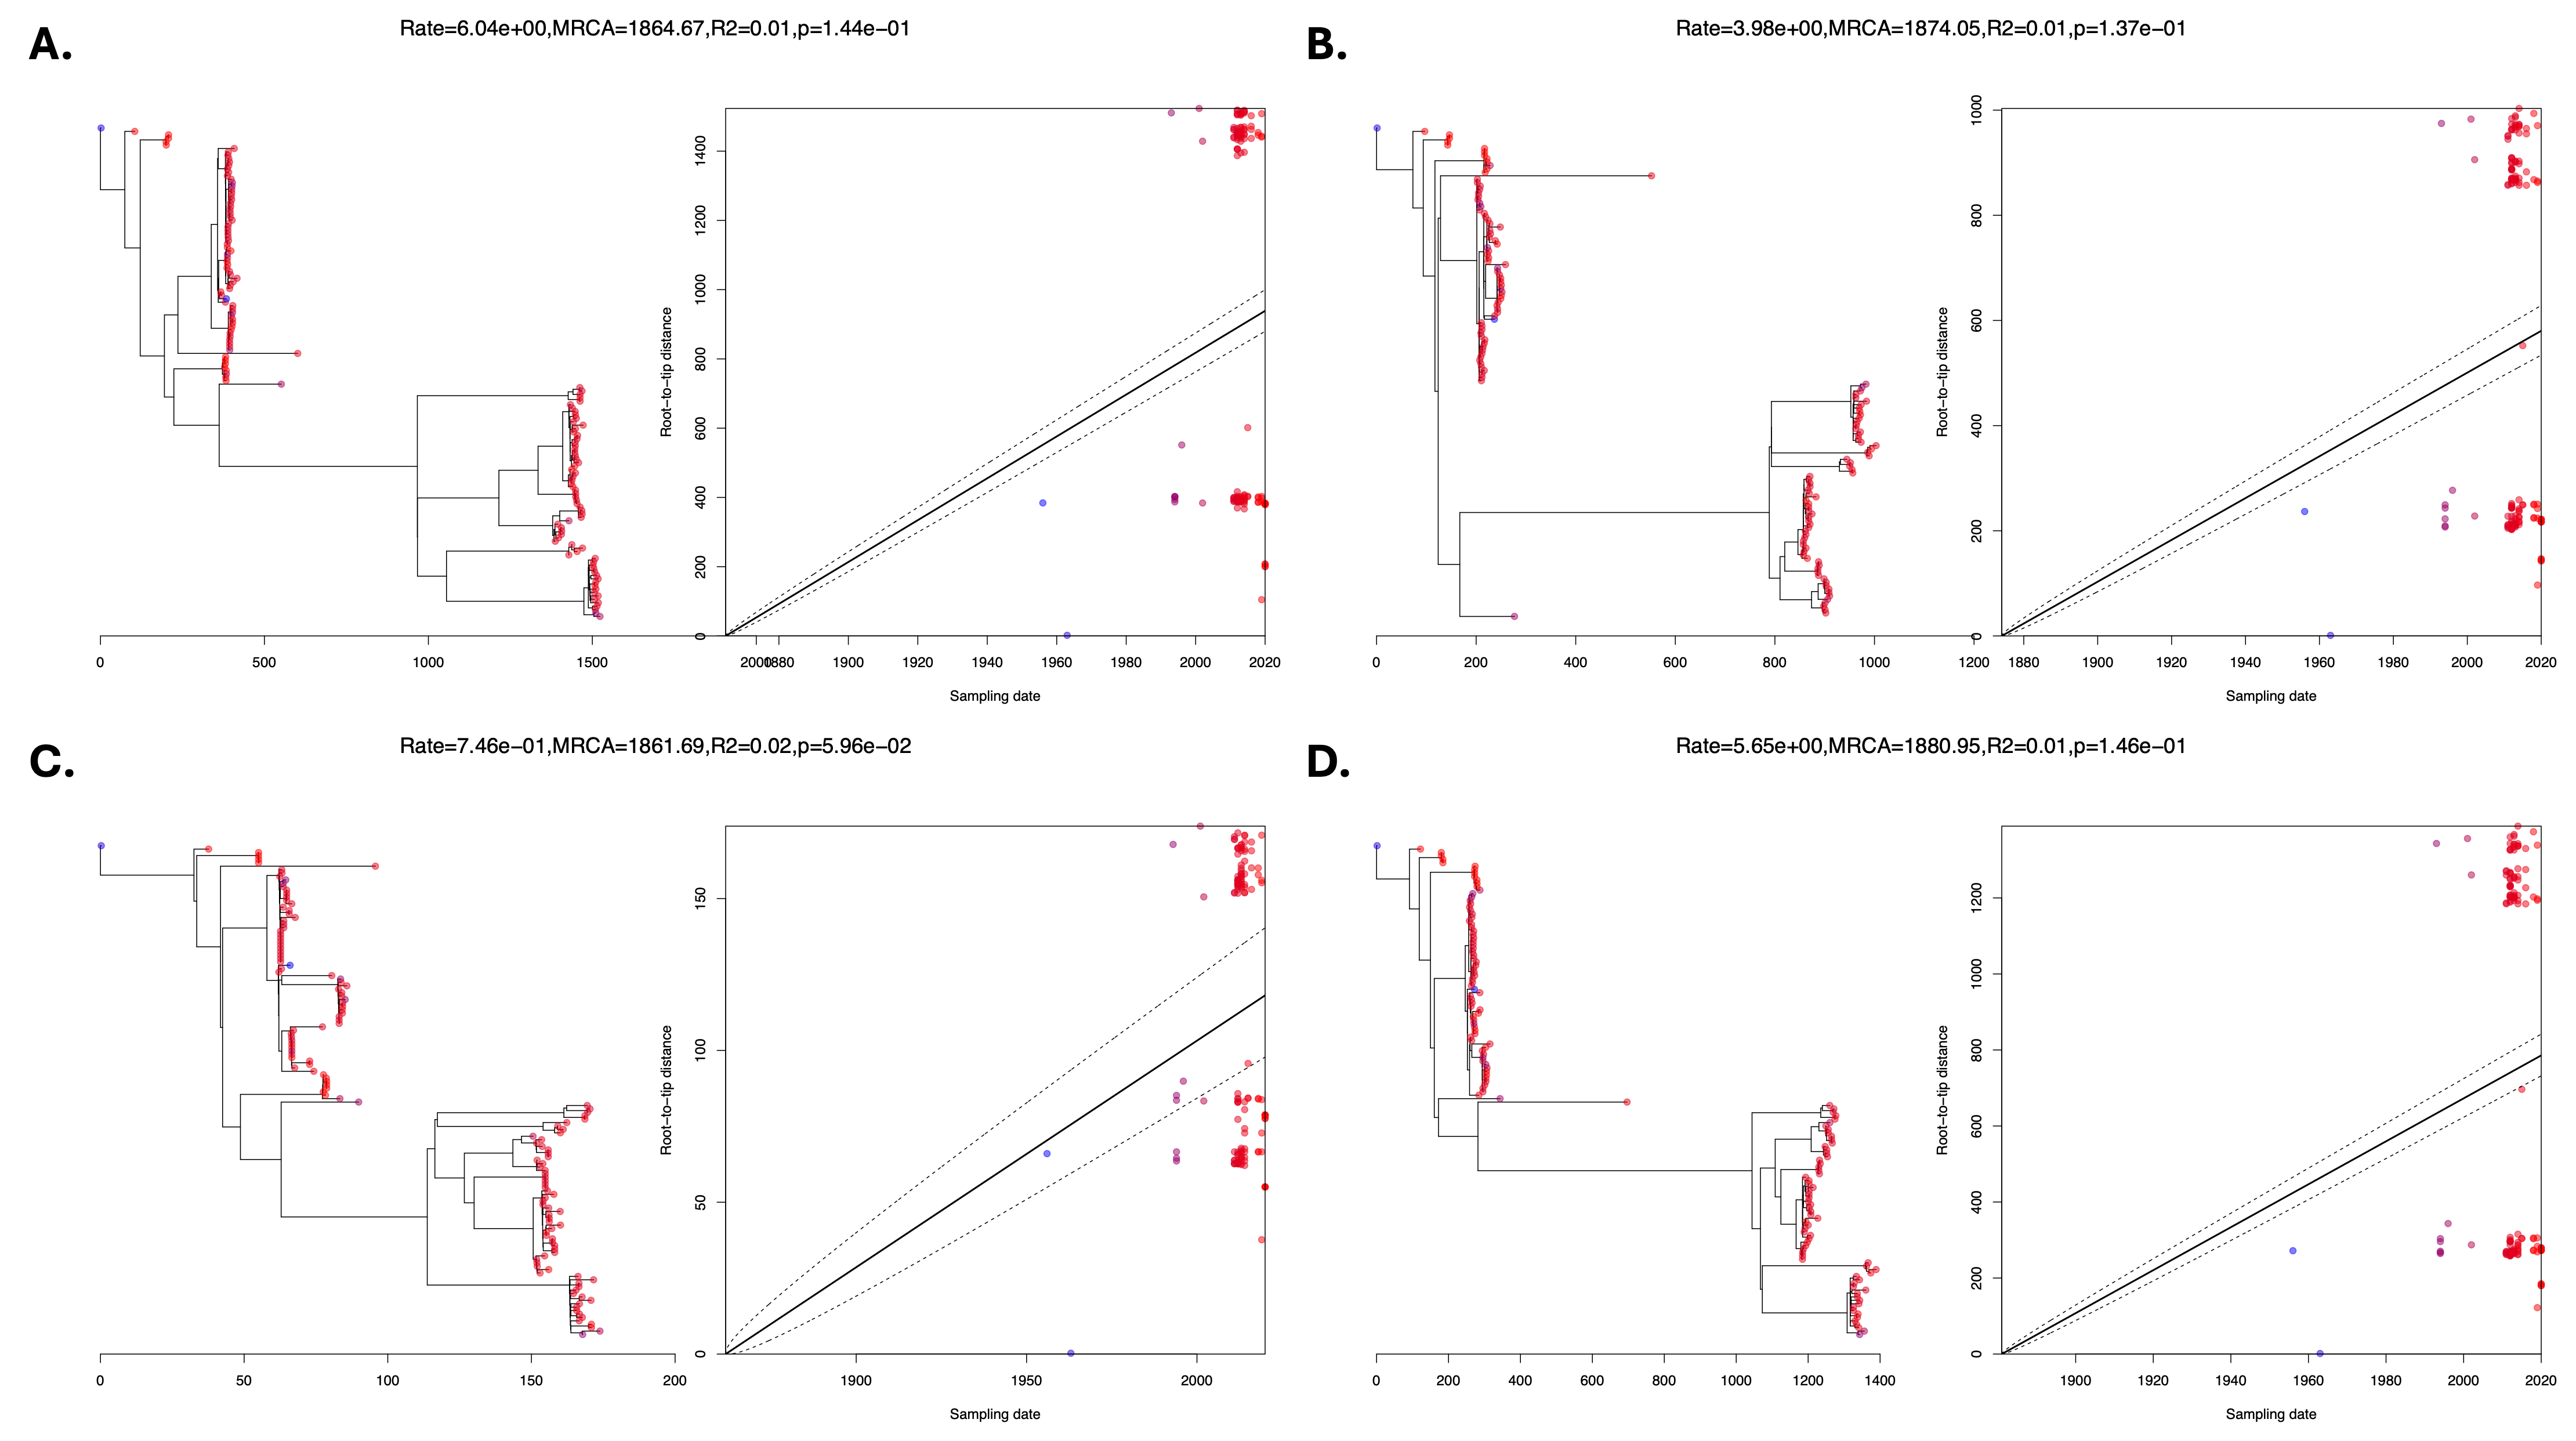
\includegraphics[width=1\linewidth,height=1\textheight]{Figures/CA_XAJ_NCBI24_Root2tip} 

}

\caption{Root-to-tip regression analysis on CA\_XAJ\_NCBI\_24 using BactDating. \textbf{A.} ClonalFrameML. \textbf{B.} Gubbins. \textbf{C.} ClonalFrameML and IQtree. \textbf{D.} ClonalFrameML and Gubbins}\label{fig:CAXAJNCBI24R2T}
\end{figure}

\chapter{Scripts}\label{Scripts}

\section{Read Processing}\label{read-processing-2}

\subsection{FastP.sh}\label{fastp-script}

\begin{Shaded}
\begin{Highlighting}[]
\CommentTok{\#!/bin/bash {-}l}

\CommentTok{\#SBATCH {-}{-}nodes=1}
\CommentTok{\#SBATCH {-}{-}cpus{-}per{-}task=4}
\CommentTok{\#SBATCH{-}{-}mem=16G}
\CommentTok{\#SBATCH {-}{-}time=7{-}00:00:00}
\CommentTok{\#\#SBATCH {-}{-}output=my.stdout}
\CommentTok{\#SBATCH {-}{-}mail{-}user=ashan007@ucr.edu}
\CommentTok{\#SBATCH {-}{-}mail{-}type=ALL}
\CommentTok{\#SBATCH {-}{-}job{-}name="FastP"}
\CommentTok{\#SBATCH {-}p batch}

\CommentTok{\# Setting sample files}
\VariableTok{SAMPFILE}\OperatorTok{=}\NormalTok{/bigdata/adaskaveglab/ashan007/Scripts/Strain\_CSV/Strains.csv}
\CommentTok{\# Setting Output directory variables}
\VariableTok{FILTERED}\OperatorTok{=}\NormalTok{/bigdata/adaskaveglab/ashan007/Filtered\_Reads}
\VariableTok{REPORTS}\OperatorTok{=}\NormalTok{/bigdata/adaskaveglab/ashan007/FastP\_Reports}
\VariableTok{IFS}\OperatorTok{=}\NormalTok{,}
\CommentTok{\# Run FastP v.0.23.4}
\FunctionTok{tail} \AttributeTok{{-}n}\NormalTok{ +2 }\VariableTok{$SAMPFILE} \KeywordTok{|} \ControlFlowTok{while} \BuiltInTok{read} \VariableTok{SID} \VariableTok{STRAIN} \VariableTok{READ1} \VariableTok{READ2} \VariableTok{ORGANISM} 
\ControlFlowTok{do}
  \ExtensionTok{/bigdata/adaskaveglab/ashan007/Programs/fastp} \DataTypeTok{\textbackslash{}}
  \AttributeTok{{-}i} \VariableTok{$READ1} \AttributeTok{{-}I} \VariableTok{$READ2} \DataTypeTok{\textbackslash{}}
  \AttributeTok{{-}o} \VariableTok{$FILTERED}\NormalTok{/}\VariableTok{$SID}\NormalTok{.F.1.fq.gz }\AttributeTok{{-}O} \VariableTok{$FILTERED}\NormalTok{/}\VariableTok{$SID}\NormalTok{.F.2.fq.gz }\DataTypeTok{\textbackslash{}}
  \AttributeTok{{-}q}\NormalTok{ 30 }\DataTypeTok{\textbackslash{}}
  \AttributeTok{{-}{-}detect\_adapter\_for\_pe} \DataTypeTok{\textbackslash{}}
  \AttributeTok{{-}h} \VariableTok{$REPORTS}\NormalTok{/}\VariableTok{$SID}\NormalTok{.html}
\ControlFlowTok{done}
\end{Highlighting}
\end{Shaded}

\section{De Novo Genome Assembly}\label{de-novo-genome-assembly}

\subsection{Step1.Assemble.sh}\label{Assemble-script}

\begin{Shaded}
\begin{Highlighting}[]
\CommentTok{\#!/bin/bash {-}l}

\CommentTok{\#SBATCH {-}{-}nodes=1}
\CommentTok{\#SBATCH {-}{-}ntasks=1}
\CommentTok{\#SBATCH {-}{-}cpus{-}per{-}task=16}
\CommentTok{\#SBATCH {-}{-}mem=64G}
\CommentTok{\#SBATCH {-}{-}time=14{-}00:00:00}
\CommentTok{\#\#SBATCH {-}{-}output=my.stdout}
\CommentTok{\#SBATCH {-}{-}mail{-}user=ashan007@ucr.edu}
\CommentTok{\#SBATCH {-}{-}mail{-}type=ALL}
\CommentTok{\#SBATCH {-}{-}job{-}name="Step 1"}
\CommentTok{\#SBATCH {-}p batch}
\CommentTok{\#SBATCH {-}{-}array 1{-}140}

\CommentTok{\#\#\#\#\#\#\#\#\#\#\#\#\#\#\#\#\#\#\#\#\#\#\#\#\#\#\#\#\#\#\#\#\#\#\#\#\#\#\#\#\#\#\#\#\#\#\#\#\#\#\#\#\#\#\#\#\#\#\#\#\#\#\#\#\#\#\#\#\#\#\#\#\#\#\#\#\#\#\#\#\#\#}
\CommentTok{\#\#\#\#\#\#\#\#\#\#\#\#\#\#\#\#\#\#\#\#\#\#\#\#\#\#\#\#\#\#\#\#\# Load Modules \#\#\#\#\#\#\#\#\#\#\#\#\#\#\#\#\#\#\#\#\#\#\#\#\#\#\#\#\#\#\#\#\#\#\#}
\CommentTok{\#\#\#\#\#\#\#\#\#\#\#\#\#\#\#\#\#\#\#\#\#\#\#\#\#\#\#\#\#\#\#\#\#\#\#\#\#\#\#\#\#\#\#\#\#\#\#\#\#\#\#\#\#\#\#\#\#\#\#\#\#\#\#\#\#\#\#\#\#\#\#\#\#\#\#\#\#\#\#\#\#\#}
\ExtensionTok{module}\NormalTok{ load quast/5.1.0rc1}
\CommentTok{\#\#\#\#\#\#\#\#\#\#\#\#\#\#\#\#\#\#\#\#\#\#\#\#\#\#\#\#\#\#\#\#\#\#\#\#\#\#\#\#\#\#\#\#\#\#\#\#\#\#\#\#\#\#\#\#\#\#\#\#\#\#\#\#\#\#\#\#\#\#\#\#\#\#\#\#\#\#\#\#\#\#}
\CommentTok{\#\#\#\#\#\#\#\#\#\#\#\#\#\#\#\#\#\#\#\#\#\#\#\#\#\#\#\#\#\#\# Define Variables \#\#\#\#\#\#\#\#\#\#\#\#\#\#\#\#\#\#\#\#\#\#\#\#\#\#\#\#\#\#\#\#\#}
\CommentTok{\#\#\#\#\#\#\#\#\#\#\#\#\#\#\#\#\#\#\#\#\#\#\#\#\#\#\#\#\#\#\#\#\#\#\#\#\#\#\#\#\#\#\#\#\#\#\#\#\#\#\#\#\#\#\#\#\#\#\#\#\#\#\#\#\#\#\#\#\#\#\#\#\#\#\#\#\#\#\#\#\#\#}
\CommentTok{\# Defining Step Directories}
\VariableTok{STEP1}\OperatorTok{=}\NormalTok{/bigdata/adaskaveglab/ashan007/Assembly\_Workflow\_PlatanusB/Step1\_Assembly/Results}
\VariableTok{STATS}\OperatorTok{=}\NormalTok{/bigdata/adaskaveglab/ashan007/Assembly\_Workflow\_PlatanusB/Step1\_Assembly/Stats}
\VariableTok{SAMPFILE}\OperatorTok{=}\NormalTok{/bigdata/adaskaveglab/ashan007/Scripts/Strain\_CSV/Assembly\_Workflow\_Platanus\_B.csv }
\VariableTok{SCAFFOLD}\OperatorTok{=}\NormalTok{/bigdata/adaskaveglab/ashan007/Scripts/Assembly\_Workflow\_PlatanusB}

\CommentTok{\# Defining Program paths}
\VariableTok{PLATANUS}\OperatorTok{=}\NormalTok{/bigdata/adaskaveglab/ashan007/Programs/Platanus\_B{-}1.3.2}
\CommentTok{\#\#\#\#\#\#\#\#\#\#\#\#\#\#\#\#\#\#\#\#\#\#\#\#\#\#\#\#\#\#\#\#\#\#\#\#\#\#\#\#\#\#\#\#\#\#\#\#\#\#\#\#\#\#\#\#\#\#\#\#\#\#\#\#\#\#\#\#\#\#\#\#\#\#\#\#\#\#\#\#\#\#}
\CommentTok{\#\#\#\#\#\#\#\#\#\#\#\#\#\#\#\#\#\#\#\#\#\#\#\#\#\#\#\#\#\#\# Define Array Vars \#\#\#\#\#\#\#\#\#\#\#\#\#\#\#\#\#\#\#\#\#\#\#\#\#\#\#\#\#\#\#\#}
\CommentTok{\#\#\#\#\#\#\#\#\#\#\#\#\#\#\#\#\#\#\#\#\#\#\#\#\#\#\#\#\#\#\#\#\#\#\#\#\#\#\#\#\#\#\#\#\#\#\#\#\#\#\#\#\#\#\#\#\#\#\#\#\#\#\#\#\#\#\#\#\#\#\#\#\#\#\#\#\#\#\#\#\#\#}
\VariableTok{CPU}\OperatorTok{=}\NormalTok{1}

\ControlFlowTok{if} \BuiltInTok{[} \VariableTok{$SLURM\_CPUS\_ON\_NODE} \BuiltInTok{]}\KeywordTok{;} \ControlFlowTok{then}
 \VariableTok{CPU}\OperatorTok{=}\VariableTok{$SLURM\_CPUS\_ON\_NODE}
\ControlFlowTok{fi}

\VariableTok{N}\OperatorTok{=}\VariableTok{$\{SLURM\_ARRAY\_TASK\_ID\}}

\ControlFlowTok{if} \BuiltInTok{[} \OtherTok{!} \VariableTok{$N} \BuiltInTok{]}\KeywordTok{;} \ControlFlowTok{then}
 \VariableTok{N}\OperatorTok{=}\VariableTok{$1}
\ControlFlowTok{fi}

\ControlFlowTok{if} \BuiltInTok{[} \OtherTok{!} \VariableTok{$N} \BuiltInTok{]}\KeywordTok{;} \ControlFlowTok{then}
 \BuiltInTok{echo} \StringTok{"need to provide a number by {-}{-}array slurm or on the cmdline"}
 \BuiltInTok{exit}
\ControlFlowTok{fi}
\CommentTok{\#\#\#\#\#\#\#\#\#\#\#\#\#\#\#\#\#\#\#\#\#\#\#\#\#\#\#\#\#\#\#\#\#\#\#\#\#\#\#\#\#\#\#\#\#\#\#\#\#\#\#\#\#\#\#\#\#\#\#\#\#\#\#\#\#\#\#\#\#\#\#\#\#\#\#\#\#\#\#\#\#\#\#\#\#\#\#\#\#\#\#\#\#\#\#\#\#\#\#\#\#\#\#\#\#\#\#\#\#\#\#\#\#\#\#\#\#\#\#\#\#\#\#}
\CommentTok{\#                                                   Begin Pipeline                                                        \#}
\CommentTok{\#\#\#\#\#\#\#\#\#\#\#\#\#\#\#\#\#\#\#\#\#\#\#\#\#\#\#\#\#\#\#\#\#\#\#\#\#\#\#\#\#\#\#\#\#\#\#\#\#\#\#\#\#\#\#\#\#\#\#\#\#\#\#\#\#\#\#\#\#\#\#\#\#\#\#\#\#\#\#\#\#\#\#\#\#\#\#\#\#\#\#\#\#\#\#\#\#\#\#\#\#\#\#\#\#\#\#\#\#\#\#\#\#\#\#\#\#\#\#\#\#\#\#}
\VariableTok{IFS}\OperatorTok{=}\NormalTok{,}
\FunctionTok{tail} \AttributeTok{{-}n}\NormalTok{ +2 }\StringTok{"}\VariableTok{$SAMPFILE}\StringTok{"} \KeywordTok{|} \FunctionTok{sed} \AttributeTok{{-}n} \StringTok{"}\VariableTok{$\{N\}}\StringTok{p"} \KeywordTok{|} \ControlFlowTok{while} \BuiltInTok{read} \AttributeTok{{-}r} \VariableTok{SID} \VariableTok{STRAIN} \VariableTok{READ1} \VariableTok{READ2} \VariableTok{ORGANISM}\KeywordTok{;} \ControlFlowTok{do}
  \CommentTok{\#\#\#\#\#\#\#\#\#\#\#\#\#\#\#\#\#\#\#\#\#\#\#\#\#\#\#\#\#\#\#\#\#\#\#\#\#\#\#\#\#\#\#\#\#\#\#\#\#\#\#\#\#\#\#\#\#\#\#\#\#\#\#\#\#\#\#\#\#\#\#\#\#\#\#\#\#\#\#\#\#\#\#\#\#\#\#\#\#\#\#\#\#\#\#\#\#\#\#\#\#\#\#\#\#\#\#\#\#\#\#\#\#\#\#\#\#\#\#\#\#\#\#}
  \CommentTok{\#\#\#\#\#\#\#\#\#\#\#\#\#\#\#\#\#\#\#\#\#\#\#\#\#\#\#\#\#\#\#\#\#\#\#\#\#\#\#\#\#\#\#\#\#\#\#\#\#\#\#\#\#\#\#\#\#\#\#\#\#\#\#\#\#\#\#\#\#\#\#\#\#\#\#\#\#\#\#\#\#\#\#\#\#\#\#\#\#\#\#\#\#\#\#\#\#\#\#\#\#\#\#\#\#\#\#\#\#\#\#\#\#\#\#\#\#\#\#\#\#\#\#}
  \CommentTok{\#                                     Step 2 Generate Assembly via Platanus\_B                                             \#}
  \CommentTok{\#\#\#\#\#\#\#\#\#\#\#\#\#\#\#\#\#\#\#\#\#\#\#\#\#\#\#\#\#\#\#\#\#\#\#\#\#\#\#\#\#\#\#\#\#\#\#\#\#\#\#\#\#\#\#\#\#\#\#\#\#\#\#\#\#\#\#\#\#\#\#\#\#\#\#\#\#\#\#\#\#\#\#\#\#\#\#\#\#\#\#\#\#\#\#\#\#\#\#\#\#\#\#\#\#\#\#\#\#\#\#\#\#\#\#\#\#\#\#\#\#\#\#}
  \CommentTok{\#\#\#\#\#\#\#\#\#\#\#\#\#\#\#\#\#\#\#\#\#\#\#\#\#\#\#\#\#\#\#\#\#\#\#\#\#\#\#\#\#\#\#\#\#\#\#\#\#\#\#\#\#\#\#\#\#\#\#\#\#\#\#\#\#\#\#\#\#\#\#\#\#\#\#\#\#\#\#\#\#\#\#\#\#\#\#\#\#\#\#\#\#\#\#\#\#\#\#\#\#\#\#\#\#\#\#\#\#\#\#\#\#\#\#\#\#\#\#\#\#\#\#}
  \ControlFlowTok{if} \BuiltInTok{[} \OtherTok{{-}d} \StringTok{"}\VariableTok{$STEP1}\StringTok{/}\VariableTok{$STRAIN}\StringTok{"} \BuiltInTok{]}\KeywordTok{;} \ControlFlowTok{then}
    \BuiltInTok{echo} \StringTok{"Skipping }\VariableTok{$STRAIN}\StringTok{ {-} Directory already exists"}
    \ControlFlowTok{continue}  \CommentTok{\# Skip to the next iteration if directory exists}
  \ControlFlowTok{else}
    \CommentTok{\# Create the directory and check if the command succeeds}
    \ControlFlowTok{if} \FunctionTok{mkdir} \AttributeTok{{-}p} \StringTok{"}\VariableTok{$STEP1}\StringTok{/}\VariableTok{$STRAIN}\StringTok{"}\KeywordTok{;} \ControlFlowTok{then}
      \BuiltInTok{echo} \StringTok{"Processing }\VariableTok{$STRAIN}\StringTok{ via Platanus\_B... STEP 1"}

      \VariableTok{$PLATANUS}\ExtensionTok{/./platanus\_b}\NormalTok{ assemble }\DataTypeTok{\textbackslash{}}
      \AttributeTok{{-}o} \StringTok{"}\VariableTok{$STEP1}\StringTok{/}\VariableTok{$STRAIN}\StringTok{/}\VariableTok{$STRAIN}\StringTok{"} \DataTypeTok{\textbackslash{}}
      \AttributeTok{{-}f} \StringTok{"}\VariableTok{$READ1}\StringTok{"} \StringTok{"}\VariableTok{$READ2}\StringTok{"} \DataTypeTok{\textbackslash{}}
      \AttributeTok{{-}t}\NormalTok{ 16 }\AttributeTok{{-}m}\NormalTok{ 64}
    \ControlFlowTok{else}
      \BuiltInTok{echo} \StringTok{"Error: Failed to create directory "}\VariableTok{$STEP1}\NormalTok{/}\VariableTok{$STRAIN}\StringTok{""}
    \ControlFlowTok{fi}
  \ControlFlowTok{fi}
  \CommentTok{\#\#\#\#\#\#\#\#\#\#\#\#\#\#\#\#\#\#\#\#\#\#\#\#\#\#\#\#\#\#\#\#\#\#\#\#\#\#\#\#\#\#\#\#\#\#\#\#\#\#\#\#\#\#\#\#\#\#\#\#\#\#\#\#\#\#\#\#\#\#\#\#\#\#\#\#\#\#\#\#\#\#\#\#\#\#\#\#\#\#\#\#\#\#\#\#\#\#\#\#\#\#\#\#\#\#\#\#\#\#\#\#\#\#\#\#\#\#\#\#\#\#\#}
  \CommentTok{\#\#\#\#\#\#\#\#\#\#\#\#\#\#\#\#\#\#\#\#\#\#\#\#\#\#\#\#\#\#\#\#\#\#\#\#\#\#\#\#\#\#\#\#\#\#\#\#\#\#\#\#\#\#\#\#\#\#\#\#\#\#\#\#\#\#\#\#\#\#\#\#\#\#\#\#\#\#\#\#\#\#\#\#\#\#\#\#\#\#\#\#\#\#\#\#\#\#\#\#\#\#\#\#\#\#\#\#\#\#\#\#\#\#\#\#\#\#\#\#\#\#\#}
  \CommentTok{\#                                     Generate Assembly Statistics via QUAST                                              \#}
  \CommentTok{\#\#\#\#\#\#\#\#\#\#\#\#\#\#\#\#\#\#\#\#\#\#\#\#\#\#\#\#\#\#\#\#\#\#\#\#\#\#\#\#\#\#\#\#\#\#\#\#\#\#\#\#\#\#\#\#\#\#\#\#\#\#\#\#\#\#\#\#\#\#\#\#\#\#\#\#\#\#\#\#\#\#\#\#\#\#\#\#\#\#\#\#\#\#\#\#\#\#\#\#\#\#\#\#\#\#\#\#\#\#\#\#\#\#\#\#\#\#\#\#\#\#\#}
  \CommentTok{\#\#\#\#\#\#\#\#\#\#\#\#\#\#\#\#\#\#\#\#\#\#\#\#\#\#\#\#\#\#\#\#\#\#\#\#\#\#\#\#\#\#\#\#\#\#\#\#\#\#\#\#\#\#\#\#\#\#\#\#\#\#\#\#\#\#\#\#\#\#\#\#\#\#\#\#\#\#\#\#\#\#\#\#\#\#\#\#\#\#\#\#\#\#\#\#\#\#\#\#\#\#\#\#\#\#\#\#\#\#\#\#\#\#\#\#\#\#\#\#\#\#\#}

  \ControlFlowTok{if} \BuiltInTok{[} \OtherTok{{-}d} \StringTok{"}\VariableTok{$STATS}\StringTok{/Contigs/}\VariableTok{$STRAIN}\StringTok{"} \BuiltInTok{]}\KeywordTok{;} \ControlFlowTok{then}
    \BuiltInTok{echo} \StringTok{"Skipping }\VariableTok{$STRAIN}\StringTok{ {-} Directory already exists"}
    \ControlFlowTok{continue}  \CommentTok{\# Skip to the next iteration if directory exists}
  \ControlFlowTok{else}
    \CommentTok{\# Create the directory and check if the command succeeds}
    \ControlFlowTok{if} \FunctionTok{mkdir} \AttributeTok{{-}p} \StringTok{"}\VariableTok{$STATS}\StringTok{/Contigs/}\VariableTok{$STRAIN}\StringTok{"}\KeywordTok{;} \ControlFlowTok{then}
      \BuiltInTok{echo} \StringTok{"Processing }\VariableTok{$STRAIN}\StringTok{ via QUAST... STEP 2"}
      \CommentTok{\# Contigs}
      \ExtensionTok{quast.py} \StringTok{"}\VariableTok{$STEP1}\StringTok{/}\VariableTok{$STRAIN}\StringTok{/}\VariableTok{$\{STRAIN\}}\StringTok{\_contig.fa"} \AttributeTok{{-}o} \StringTok{"}\VariableTok{$STATS}\StringTok{/Contigs/}\VariableTok{$STRAIN}\StringTok{"}
    \ControlFlowTok{else}
      \BuiltInTok{echo} \StringTok{"Error: Failed to create directory "}\VariableTok{$STATS}\NormalTok{/Contigs/}\VariableTok{$STRAIN}\StringTok{""}
    \ControlFlowTok{fi}
  \ControlFlowTok{fi}
\ControlFlowTok{done}
\end{Highlighting}
\end{Shaded}

\subsection{Summarize\_ANI.sh}\label{ANI-script}

\begin{Shaded}
\begin{Highlighting}[]
\CommentTok{\#!/bin/bash}

\CommentTok{\# Initialize the output file with the header}
\BuiltInTok{echo} \AttributeTok{{-}e} \StringTok{"Sample\textbackslash{}tAssembly\textbackslash{}tSubmitted Organism\textbackslash{}tPredicted Organism\textbackslash{}tSubmitted Type\textbackslash{}tStatus\textbackslash{}tConfidence\textbackslash{}tBest Hit"} \OperatorTok{\textgreater{}}\NormalTok{ ani\_summary\_table.tsv}

\CommentTok{\# Loop over each subdirectory}
\ControlFlowTok{for}\NormalTok{ dir }\KeywordTok{in} \PreprocessorTok{*}\NormalTok{/}\KeywordTok{;} \ControlFlowTok{do}
    \CommentTok{\# Check if the directory contains the ani{-}tax{-}report.txt file}
    \ControlFlowTok{if} \KeywordTok{[[} \OtherTok{{-}f} \StringTok{"}\VariableTok{$\{dir\}}\StringTok{ani{-}tax{-}report.txt"} \KeywordTok{]];} \ControlFlowTok{then}
        \CommentTok{\# Extract the relevant lines from the ani{-}tax{-}report.txt file}
        \VariableTok{assembly}\OperatorTok{=}\VariableTok{$(}\FunctionTok{sed} \AttributeTok{{-}n} \StringTok{\textquotesingle{}1p\textquotesingle{}} \StringTok{"}\VariableTok{$\{dir\}}\StringTok{ani{-}tax{-}report.txt"} \KeywordTok{|} \FunctionTok{cut} \AttributeTok{{-}d}\StringTok{\textquotesingle{}:\textquotesingle{}} \AttributeTok{{-}f2} \KeywordTok{|} \FunctionTok{xargs}\VariableTok{)}
        \VariableTok{submitted\_organism}\OperatorTok{=}\VariableTok{$(}\FunctionTok{sed} \AttributeTok{{-}n} \StringTok{\textquotesingle{}2p\textquotesingle{}} \StringTok{"}\VariableTok{$\{dir\}}\StringTok{ani{-}tax{-}report.txt"} \KeywordTok{|} \FunctionTok{cut} \AttributeTok{{-}d}\StringTok{\textquotesingle{}:\textquotesingle{}} \AttributeTok{{-}f2} \KeywordTok{|} \FunctionTok{xargs}\VariableTok{)}
        \VariableTok{predicted\_organism}\OperatorTok{=}\VariableTok{$(}\FunctionTok{sed} \AttributeTok{{-}n} \StringTok{\textquotesingle{}3p\textquotesingle{}} \StringTok{"}\VariableTok{$\{dir\}}\StringTok{ani{-}tax{-}report.txt"} \KeywordTok{|} \FunctionTok{cut} \AttributeTok{{-}d}\StringTok{\textquotesingle{}:\textquotesingle{}} \AttributeTok{{-}f2} \KeywordTok{|} \FunctionTok{xargs}\VariableTok{)}
        \VariableTok{submitted\_type}\OperatorTok{=}\VariableTok{$(}\FunctionTok{sed} \AttributeTok{{-}n} \StringTok{\textquotesingle{}4p\textquotesingle{}} \StringTok{"}\VariableTok{$\{dir\}}\StringTok{ani{-}tax{-}report.txt"} \KeywordTok{|} \FunctionTok{cut} \AttributeTok{{-}d}\StringTok{\textquotesingle{}:\textquotesingle{}} \AttributeTok{{-}f2} \KeywordTok{|} \FunctionTok{xargs}\VariableTok{)}
        \VariableTok{status}\OperatorTok{=}\VariableTok{$(}\FunctionTok{sed} \AttributeTok{{-}n} \StringTok{\textquotesingle{}5p\textquotesingle{}} \StringTok{"}\VariableTok{$\{dir\}}\StringTok{ani{-}tax{-}report.txt"} \KeywordTok{|} \FunctionTok{cut} \AttributeTok{{-}d}\StringTok{\textquotesingle{}:\textquotesingle{}} \AttributeTok{{-}f2} \KeywordTok{|} \FunctionTok{xargs}\VariableTok{)}
        \VariableTok{confidence}\OperatorTok{=}\VariableTok{$(}\FunctionTok{sed} \AttributeTok{{-}n} \StringTok{\textquotesingle{}6p\textquotesingle{}} \StringTok{"}\VariableTok{$\{dir\}}\StringTok{ani{-}tax{-}report.txt"} \KeywordTok{|} \FunctionTok{cut} \AttributeTok{{-}d}\StringTok{\textquotesingle{}:\textquotesingle{}} \AttributeTok{{-}f2} \KeywordTok{|} \FunctionTok{xargs}\VariableTok{)}

        \CommentTok{\# Capture the ANI value from the first data row under the dashed line following the "ANI" header}
        \VariableTok{best\_hit}\OperatorTok{=}\VariableTok{$(}\FunctionTok{awk} \StringTok{\textquotesingle{}/\^{}{-}{-}{-}{-}{-}{-}{-}/\{getline; print $1; exit\}\textquotesingle{}} \StringTok{"}\VariableTok{$\{dir\}}\StringTok{ani{-}tax{-}report.txt"} \KeywordTok{|} \FunctionTok{xargs}\VariableTok{)}
        
        \CommentTok{\# Get the directory name without the trailing slash (which is the sample name)}
        \VariableTok{sample}\OperatorTok{=}\VariableTok{$\{dir}\OperatorTok{\%}\NormalTok{/}\VariableTok{\}}
        
        \CommentTok{\# Append the data to the summary table}
        \BuiltInTok{echo} \AttributeTok{{-}e} \StringTok{"}\VariableTok{$\{sample\}}\StringTok{\textbackslash{}t}\VariableTok{$\{assembly\}}\StringTok{\textbackslash{}t}\VariableTok{$\{submitted\_organism\}}\StringTok{\textbackslash{}t}\VariableTok{$\{predicted\_organism\}}\StringTok{\textbackslash{}t}\VariableTok{$\{submitted\_type\}}\StringTok{\textbackslash{}t}\VariableTok{$\{status\}}\StringTok{\textbackslash{}t}\VariableTok{$\{confidence\}}\StringTok{\textbackslash{}t}\VariableTok{$\{best\_hit\}}\StringTok{"} \OperatorTok{\textgreater{}\textgreater{}}\NormalTok{ ani\_summary\_table.tsv}
    \ControlFlowTok{fi}
\ControlFlowTok{done}

\BuiltInTok{echo} \StringTok{"ANI summary table has been created in ani\_summary\_table.tsv"}
\end{Highlighting}
\end{Shaded}

\subsection{Summarize\_CheckM.sh}\label{CheckM-script}

\begin{Shaded}
\begin{Highlighting}[]
\CommentTok{\#!/bin/bash}

\CommentTok{\# Initialize the output file with the header}
\BuiltInTok{echo} \AttributeTok{{-}e} \StringTok{"Sample\textbackslash{}tBin Id\textbackslash{}tMarker lineage\textbackslash{}t\# genomes\textbackslash{}t\# markers\textbackslash{}t\# marker sets\textbackslash{}t0\textbackslash{}t1\textbackslash{}t2\textbackslash{}t3\textbackslash{}t4\textbackslash{}t5+\textbackslash{}tCompleteness\textbackslash{}tContamination\textbackslash{}tStrain heterogeneity"} \OperatorTok{\textgreater{}}\NormalTok{ checkm\_summary\_table.tsv}

\CommentTok{\# Loop over each subdirectory}
\ControlFlowTok{for}\NormalTok{ dir }\KeywordTok{in} \PreprocessorTok{*}\NormalTok{/}\KeywordTok{;} \ControlFlowTok{do}
    \CommentTok{\# Check if the directory contains the checkm.txt file}
    \ControlFlowTok{if} \KeywordTok{[[} \OtherTok{{-}f} \StringTok{"}\VariableTok{$\{dir\}}\StringTok{checkm.txt"} \KeywordTok{]];} \ControlFlowTok{then}
        \CommentTok{\# Extract the second line (data) from the checkm.txt file}
        \VariableTok{data}\OperatorTok{=}\VariableTok{$(}\FunctionTok{sed} \AttributeTok{{-}n} \StringTok{\textquotesingle{}2p\textquotesingle{}} \StringTok{"}\VariableTok{$\{dir\}}\StringTok{checkm.txt"}\VariableTok{)}
        \CommentTok{\# Get the directory name without the trailing slash (which is the sample name)}
        \VariableTok{sample}\OperatorTok{=}\VariableTok{$\{dir}\OperatorTok{\%}\NormalTok{/}\VariableTok{\}}
        \CommentTok{\# Append the sample name and the data to the final table}
        \BuiltInTok{echo} \AttributeTok{{-}e} \StringTok{"}\VariableTok{$\{sample\}}\StringTok{\textbackslash{}t}\VariableTok{$\{data\}}\StringTok{"} \OperatorTok{\textgreater{}\textgreater{}}\NormalTok{ checkm\_summary\_table.tsv}
    \ControlFlowTok{fi}
\ControlFlowTok{done}

\BuiltInTok{echo} \StringTok{"CheckM summary table has been created in checkm\_summary\_table.tsv"}
\end{Highlighting}
\end{Shaded}

\subsection{Summarize\_Genbank.py}\label{Genbank-script}

\begin{Shaded}
\begin{Highlighting}[]
\CommentTok{\#!/usr/bin/env python}
\CommentTok{\# coding: utf{-}8}

\ImportTok{import}\NormalTok{ os}
\ImportTok{import}\NormalTok{ re}
\ImportTok{import}\NormalTok{ pandas }\ImportTok{as}\NormalTok{ pd}

\KeywordTok{def}\NormalTok{ extract\_genome\_annotation\_data(file\_path):}
    \ControlFlowTok{try}\NormalTok{:}
        \ControlFlowTok{with} \BuiltInTok{open}\NormalTok{(file\_path, }\StringTok{\textquotesingle{}r\textquotesingle{}}\NormalTok{, encoding}\OperatorTok{=}\StringTok{\textquotesingle{}utf{-}8\textquotesingle{}}\NormalTok{, errors}\OperatorTok{=}\StringTok{\textquotesingle{}ignore\textquotesingle{}}\NormalTok{) }\ImportTok{as} \BuiltInTok{file}\NormalTok{:}
\NormalTok{            content }\OperatorTok{=} \BuiltInTok{file}\NormalTok{.read()}
    \ControlFlowTok{except} \PreprocessorTok{UnicodeDecodeError}\NormalTok{:}
        \BuiltInTok{print}\NormalTok{(}\SpecialStringTok{f"Failed to decode file: }\SpecialCharTok{\{}\NormalTok{file\_path}\SpecialCharTok{\}}\SpecialStringTok{"}\NormalTok{)}
        \ControlFlowTok{return} \VariableTok{None}
    
    \CommentTok{\# Find the section starting with "\#Genome{-}Annotation{-}Data{-}START\#\#"}
\NormalTok{    start\_index }\OperatorTok{=}\NormalTok{ content.find(}\StringTok{"\#Genome{-}Annotation{-}Data{-}START\#\#"}\NormalTok{)}
    \ControlFlowTok{if}\NormalTok{ start\_index }\OperatorTok{==} \OperatorTok{{-}}\DecValTok{1}\NormalTok{:}
        \BuiltInTok{print}\NormalTok{(}\SpecialStringTok{f"Section not found in file: }\SpecialCharTok{\{}\NormalTok{file\_path}\SpecialCharTok{\}}\SpecialStringTok{"}\NormalTok{)}
        \ControlFlowTok{return} \VariableTok{None}  \CommentTok{\# Section not found}
    
    \CommentTok{\# Extract the section}
\NormalTok{    section }\OperatorTok{=}\NormalTok{ content[start\_index:]}
    
    \CommentTok{\# Define the keys to extract}
\NormalTok{    keys }\OperatorTok{=}\NormalTok{ [}
        \StringTok{"Genes (total)"}\NormalTok{, }\StringTok{"CDSs (total)"}\NormalTok{, }\StringTok{"Genes (coding)"}\NormalTok{, }
        \StringTok{"CDSs (with protein)"}\NormalTok{, }\StringTok{"Genes (RNA)"}\NormalTok{, }\StringTok{"rRNAs"}\NormalTok{, }
        \StringTok{"complete rRNAs"}\NormalTok{, }\StringTok{"partial rRNAs"}\NormalTok{, }\StringTok{"tRNAs"}\NormalTok{, }
        \StringTok{"ncRNAs"}\NormalTok{, }\StringTok{"Pseudo Genes (total)"}\NormalTok{, }\StringTok{"CDSs (without protein)"}
\NormalTok{    ]}
    
\NormalTok{    data }\OperatorTok{=}\NormalTok{ \{\}}
    \ControlFlowTok{for}\NormalTok{ key }\KeywordTok{in}\NormalTok{ keys:}
\NormalTok{        match }\OperatorTok{=}\NormalTok{ re.search(}\VerbatimStringTok{rf"}\SpecialCharTok{\{}\NormalTok{re}\SpecialCharTok{.}\NormalTok{escape(key)}\SpecialCharTok{\}}\VerbatimStringTok{\textbackslash{}s*::\textbackslash{}s*(.+)"}\NormalTok{, section)}
        \ControlFlowTok{if}\NormalTok{ match:}
\NormalTok{            value }\OperatorTok{=}\NormalTok{ match.group(}\DecValTok{1}\NormalTok{).strip()}
            \CommentTok{\# Convert values to int if possible}
            \ControlFlowTok{try}\NormalTok{:}
\NormalTok{                value }\OperatorTok{=} \BuiltInTok{int}\NormalTok{(value.replace(}\StringTok{\textquotesingle{},\textquotesingle{}}\NormalTok{, }\StringTok{\textquotesingle{}\textquotesingle{}}\NormalTok{))}
            \ControlFlowTok{except} \PreprocessorTok{ValueError}\NormalTok{:}
                \ControlFlowTok{pass}
\NormalTok{            data[key] }\OperatorTok{=}\NormalTok{ value}
        \ControlFlowTok{else}\NormalTok{:}
\NormalTok{            data[key] }\OperatorTok{=} \VariableTok{None}  \CommentTok{\# Key not found or no value}
            \BuiltInTok{print}\NormalTok{(}\SpecialStringTok{f"Key \textquotesingle{}}\SpecialCharTok{\{}\NormalTok{key}\SpecialCharTok{\}}\SpecialStringTok{\textquotesingle{} not found in section of file: }\SpecialCharTok{\{}\NormalTok{file\_path}\SpecialCharTok{\}}\SpecialStringTok{"}\NormalTok{)}
    
    \ControlFlowTok{return}\NormalTok{ data}

\KeywordTok{def}\NormalTok{ process\_genbank\_files(base\_directory):}
\NormalTok{    result }\OperatorTok{=}\NormalTok{ []}
    \CommentTok{\# Iterate over each subdirectory}
    \ControlFlowTok{for}\NormalTok{ root, dirs, files }\KeywordTok{in}\NormalTok{ os.walk(base\_directory):}
        \ControlFlowTok{for}\NormalTok{ filename }\KeywordTok{in}\NormalTok{ files:}
            \ControlFlowTok{if}\NormalTok{ filename.endswith(}\StringTok{".gbk"}\NormalTok{):}
\NormalTok{                sample\_name }\OperatorTok{=}\NormalTok{ os.path.basename(root)  }\CommentTok{\# Get the subdirectory name as sample name}
\NormalTok{                file\_path }\OperatorTok{=}\NormalTok{ os.path.join(root, filename)}
\NormalTok{                data }\OperatorTok{=}\NormalTok{ extract\_genome\_annotation\_data(file\_path)}
                \ControlFlowTok{if}\NormalTok{ data:}
                    \CommentTok{\# Add the sample name to the data}
\NormalTok{                    data[}\StringTok{\textquotesingle{}Sample\textquotesingle{}}\NormalTok{] }\OperatorTok{=}\NormalTok{ sample\_name}
\NormalTok{                    result.append(data)}
                \ControlFlowTok{else}\NormalTok{:}
                    \BuiltInTok{print}\NormalTok{(}\SpecialStringTok{f"No data extracted from file: }\SpecialCharTok{\{}\NormalTok{file\_path}\SpecialCharTok{\}}\SpecialStringTok{"}\NormalTok{)}
    
    \ControlFlowTok{return}\NormalTok{ result}

\KeywordTok{def}\NormalTok{ main():}
\NormalTok{    base\_directory }\OperatorTok{=} \StringTok{"/Volumes/AS\_Postdoc/Postdoc2024/Assembly\_Workflow\_PlatanusB/Step4\_Annotate/Step2\_Annotate/Results"}  \CommentTok{\# Replace with the path to your subdirectories}
\NormalTok{    data }\OperatorTok{=}\NormalTok{ process\_genbank\_files(base\_directory)}
    
    \ControlFlowTok{if}\NormalTok{ data:}
        \CommentTok{\# Convert the list of dictionaries to a pandas DataFrame}
\NormalTok{        df }\OperatorTok{=}\NormalTok{ pd.DataFrame(data)}
        
        \CommentTok{\# Reorder columns to place \textquotesingle{}Sample\textquotesingle{} at the beginning}
\NormalTok{        cols }\OperatorTok{=}\NormalTok{ [}\StringTok{\textquotesingle{}Sample\textquotesingle{}}\NormalTok{] }\OperatorTok{+}\NormalTok{ [col }\ControlFlowTok{for}\NormalTok{ col }\KeywordTok{in}\NormalTok{ df.columns }\ControlFlowTok{if}\NormalTok{ col }\OperatorTok{!=} \StringTok{\textquotesingle{}Sample\textquotesingle{}}\NormalTok{]}
\NormalTok{        df }\OperatorTok{=}\NormalTok{ df[cols]}
        
        \CommentTok{\# Save the DataFrame to a CSV file}
\NormalTok{        df.to\_csv(}\StringTok{\textquotesingle{}Genome\_Annotation\_Summary.csv\textquotesingle{}}\NormalTok{, index}\OperatorTok{=}\VariableTok{False}\NormalTok{)}
        
        \BuiltInTok{print}\NormalTok{(}\StringTok{"Genome annotation data has been extracted and saved to Genome\_Annotation\_Summary.csv"}\NormalTok{)}
    \ControlFlowTok{else}\NormalTok{:}
        \BuiltInTok{print}\NormalTok{(}\StringTok{"No genome annotation data found in the provided files."}\NormalTok{)}

\ControlFlowTok{if} \VariableTok{\_\_name\_\_} \OperatorTok{==} \StringTok{"\_\_main\_\_"}\NormalTok{:}
\NormalTok{    main()}
\end{Highlighting}
\end{Shaded}

\subsection{Generate\_RCP.sh}\label{RCP-script}

\begin{Shaded}
\begin{Highlighting}[]
\CommentTok{\#!/bin/bash}

\CommentTok{\# Set the path to your strains file}
\VariableTok{STRAINS\_FILE}\OperatorTok{=}\StringTok{"/Volumes/AS\_Postdoc/Postdoc2024/Strain\_Datasets/XAJ\_Strains.RCP.csv"} 

\CommentTok{\# Set the path to your template file}
\VariableTok{TEMPLATE\_FILE}\OperatorTok{=}\StringTok{"/Volumes/AS\_Postdoc/Postdoc2024/Ragout/Template\_RCP\_Files/Platanus\_B/XAJ\_Template.rcp"}  

\CommentTok{\# Directory to save the output .rcp files }
\VariableTok{OUTPUT\_DIR}\OperatorTok{=}\StringTok{"//Volumes/AS\_Postdoc/Postdoc2024/Assembly\_Workflow\_PlatanusB/Step2\_Scaffold/rcp\_files\_contig\_IVIA1317ref"}
\FunctionTok{mkdir} \AttributeTok{{-}p} \VariableTok{$OUTPUT\_DIR}

\CommentTok{\# Skip the header and loop through each strain in the strains file}
\FunctionTok{tail} \AttributeTok{{-}n}\NormalTok{ +2 }\StringTok{"}\VariableTok{$STRAINS\_FILE}\StringTok{"} \KeywordTok{|} \ControlFlowTok{while} \VariableTok{IFS}\OperatorTok{=}\NormalTok{, }\BuiltInTok{read} \AttributeTok{{-}r} \VariableTok{strain}\KeywordTok{;} \ControlFlowTok{do}
    \CommentTok{\# Replace $STRAIN with the actual strain name in the template file and ensure .fa stays attached}
    \FunctionTok{sed} \StringTok{"s/}\DataTypeTok{\textbackslash{}$}\StringTok{STRAIN/}\VariableTok{$strain}\StringTok{/g"} \StringTok{"}\VariableTok{$TEMPLATE\_FILE}\StringTok{"} \KeywordTok{|} \FunctionTok{sed} \StringTok{"s/}\VariableTok{$strain}\StringTok{ \textbackslash{}.fa/}\VariableTok{$strain}\StringTok{.fa/g"} \OperatorTok{\textgreater{}} \StringTok{"}\VariableTok{$OUTPUT\_DIR}\StringTok{/}\VariableTok{$strain}\StringTok{.rcp"}
    \ExtensionTok{dos2unix} \StringTok{"}\VariableTok{$OUTPUT\_DIR}\StringTok{/}\VariableTok{$strain}\StringTok{.rcp"}

    \BuiltInTok{echo} \StringTok{"Generated: }\VariableTok{$OUTPUT\_DIR}\StringTok{/}\VariableTok{$strain}\StringTok{.rcp"}
\ControlFlowTok{done}
\end{Highlighting}
\end{Shaded}

\subsection{Step2.Scaffold.sh}\label{Ragout-script}

\begin{Shaded}
\begin{Highlighting}[]
\CommentTok{\#!/bin/bash {-}l}

\CommentTok{\#SBATCH {-}{-}nodes=1}
\CommentTok{\#SBATCH {-}{-}ntasks=1}
\CommentTok{\#SBATCH {-}{-}cpus{-}per{-}task=16}
\CommentTok{\#SBATCH {-}{-}mem=64G}
\CommentTok{\#SBATCH {-}{-}time=14{-}00:00:00}
\CommentTok{\#\#SBATCH {-}{-}output=my.stdout}
\CommentTok{\#SBATCH {-}{-}mail{-}user=ashan007@ucr.edu}
\CommentTok{\#SBATCH {-}{-}mail{-}type=ALL}
\CommentTok{\#SBATCH {-}{-}job{-}name="Pipeline"}
\CommentTok{\#SBATCH {-}p batch}
\CommentTok{\#SBATCH {-}{-}array 1{-}140}

\CommentTok{\#\#\#\#\#\#\#\#\#\#\#\#\#\#\#\#\#\#\#\#\#\#\#\#\#\#\#\#\#\#\#\#\#\#\#\#\#\#\#\#\#\#\#\#\#\#\#\#\#\#\#\#\#\#\#\#\#\#\#\#\#\#\#\#\#\#\#\#\#\#\#\#\#\#\#\#\#\#\#\#\#\#}
\CommentTok{\#\#\#\#\#\#\#\#\#\#\#\#\#\#\#\#\#\#\#\#\#\#\#\#\#\#\#\#\#\#\#\#\# }\AlertTok{NOTE}\CommentTok{!!!!!!!! \#\#\#\#\#\#\#\#\#\#\#\#\#\#\#\#\#\#\#\#\#\#\#\#\#\#\#\#\#\#\#\#\#\#\#}
\CommentTok{\#\#\#\#\#\#\#\#\#\#\#\#\#\#\#\#\#\#\#\#\#\#\#\#\#\#\#\#\#\#\#\#\#\#\#\#\#\#\#\#\#\#\#\#\#\#\#\#\#\#\#\#\#\#\#\#\#\#\#\#\#\#\#\#\#\#\#\#\#\#\#\#\#\#\#\#\#\#\#\#\#\#}
\CommentTok{\# I renamed the chromosomes in the refernce fasta files used for the scaffolding }
\CommentTok{\# IVIA1317 and 15\_088) becuase Ragout will use their ID to name our strains. I do }
\CommentTok{\# not want out population to have the same NCBI assembly ID for obvious reasons so }
\CommentTok{\# I renamed the chromosome to chr1 for both. I only modified those two fastas }
\CommentTok{\# located: /bigdata/adaskaveglab/ashan007/Assembly\_Workflow/Step3\_Scaffold/References}
\CommentTok{\#\#\#\#\#\#\#\#\#\#\#\#\#\#\#\#\#\#\#\#\#\#\#\#\#\#\#\#\#\#\#\#\#\#\#\#\#\#\#\#\#\#\#\#\#\#\#\#\#\#\#\#\#\#\#\#\#\#\#\#\#\#\#\#\#\#\#\#\#\#\#\#\#\#\#\#\#\#\#\#\#\#}
\CommentTok{\#\#\#\#\#\#\#\#\#\#\#\#\#\#\#\#\#\#\#\#\#\#\#\#\#\#\#\#\#\#\#\#\# Load Modules \#\#\#\#\#\#\#\#\#\#\#\#\#\#\#\#\#\#\#\#\#\#\#\#\#\#\#\#\#\#\#\#\#\#\#}
\CommentTok{\#\#\#\#\#\#\#\#\#\#\#\#\#\#\#\#\#\#\#\#\#\#\#\#\#\#\#\#\#\#\#\#\#\#\#\#\#\#\#\#\#\#\#\#\#\#\#\#\#\#\#\#\#\#\#\#\#\#\#\#\#\#\#\#\#\#\#\#\#\#\#\#\#\#\#\#\#\#\#\#\#\#}
\CommentTok{\# module load ragout/v2.3}
\CommentTok{\# module load quast/5.1.0rc1}
\CommentTok{\#\#\#\#\#\#\#\#\#\#\#\#\#\#\#\#\#\#\#\#\#\#\#\#\#\#\#\#\#\#\#\#\#\#\#\#\#\#\#\#\#\#\#\#\#\#\#\#\#\#\#\#\#\#\#\#\#\#\#\#\#\#\#\#\#\#\#\#\#\#\#\#\#\#\#\#\#\#\#\#\#\#}
\CommentTok{\#\#\#\#\#\#\#\#\#\#\#\#\#\#\#\#\#\#\#\#\#\#\#\#\#\#\#\#\#\#\# Define Variables \#\#\#\#\#\#\#\#\#\#\#\#\#\#\#\#\#\#\#\#\#\#\#\#\#\#\#\#\#\#\#\#\#}
\CommentTok{\#\#\#\#\#\#\#\#\#\#\#\#\#\#\#\#\#\#\#\#\#\#\#\#\#\#\#\#\#\#\#\#\#\#\#\#\#\#\#\#\#\#\#\#\#\#\#\#\#\#\#\#\#\#\#\#\#\#\#\#\#\#\#\#\#\#\#\#\#\#\#\#\#\#\#\#\#\#\#\#\#\#}
\CommentTok{\# Defining Step Directories}
\VariableTok{SAMPFILE}\OperatorTok{=}\NormalTok{/bigdata/adaskaveglab/ashan007/Scripts/Strain\_CSV/Assembly\_Workflow\_Platanus\_B.csv}

\CommentTok{\# IVIA as reference with contigs}
\VariableTok{IVIACONRES}\OperatorTok{=}\NormalTok{/bigdata/adaskaveglab/ashan007/Assembly\_Workflow\_PlatanusB/Step2\_Scaffold/IVIA\_Contig\_Results}
\VariableTok{IVIACONSTATS}\OperatorTok{=}\NormalTok{/bigdata/adaskaveglab/ashan007/Assembly\_Workflow\_PlatanusB/Step2\_Scaffold/Stats/IVIA\_Contig}
\VariableTok{IVIACONRECIPEDIR}\OperatorTok{=}\NormalTok{/bigdata/adaskaveglab/ashan007/Assembly\_Workflow\_PlatanusB/Step2\_Scaffold/rcp\_files\_contig\_IVIA1317ref}

\CommentTok{\#\#\#\#\#\#\#\#\#\#\#\#\#\#\#\#\#\#\#\#\#\#\#\#\#\#\#\#\#\#\#\#\#\#\#\#\#\#\#\#\#\#\#\#\#\#\#\#\#\#\#\#\#\#\#\#\#\#\#\#\#\#\#\#\#\#\#\#\#\#\#\#\#\#\#\#\#\#\#\#\#\#}
\CommentTok{\#\#\#\#\#\#\#\#\#\#\#\#\#\#\#\#\#\#\#\#\#\#\#\#\#\#\#\#\#\#\# Define Array Vars \#\#\#\#\#\#\#\#\#\#\#\#\#\#\#\#\#\#\#\#\#\#\#\#\#\#\#\#\#\#\#\#}
\CommentTok{\#\#\#\#\#\#\#\#\#\#\#\#\#\#\#\#\#\#\#\#\#\#\#\#\#\#\#\#\#\#\#\#\#\#\#\#\#\#\#\#\#\#\#\#\#\#\#\#\#\#\#\#\#\#\#\#\#\#\#\#\#\#\#\#\#\#\#\#\#\#\#\#\#\#\#\#\#\#\#\#\#\#}
\VariableTok{CPU}\OperatorTok{=}\NormalTok{1}

\ControlFlowTok{if} \BuiltInTok{[} \VariableTok{$SLURM\_CPUS\_ON\_NODE} \BuiltInTok{]}\KeywordTok{;} \ControlFlowTok{then}
 \VariableTok{CPU}\OperatorTok{=}\VariableTok{$SLURM\_CPUS\_ON\_NODE}
\ControlFlowTok{fi}

\VariableTok{N}\OperatorTok{=}\VariableTok{$\{SLURM\_ARRAY\_TASK\_ID\}}

\ControlFlowTok{if} \BuiltInTok{[} \OtherTok{!} \VariableTok{$N} \BuiltInTok{]}\KeywordTok{;} \ControlFlowTok{then}
 \VariableTok{N}\OperatorTok{=}\VariableTok{$1}
\ControlFlowTok{fi}

\ControlFlowTok{if} \BuiltInTok{[} \OtherTok{!} \VariableTok{$N} \BuiltInTok{]}\KeywordTok{;} \ControlFlowTok{then}
 \BuiltInTok{echo} \StringTok{"need to provide a number by {-}{-}array slurm or on the cmdline"}
 \BuiltInTok{exit}
\ControlFlowTok{fi}
\CommentTok{\#\#\#\#\#\#\#\#\#\#\#\#\#\#\#\#\#\#\#\#\#\#\#\#\#\#\#\#\#\#\#\#\#\#\#\#\#\#\#\#\#\#\#\#\#\#\#\#\#\#\#\#\#\#\#\#\#\#\#\#\#\#\#\#\#\#\#\#\#\#\#\#\#\#\#\#\#\#\#\#\#\#\#\#\#\#\#\#\#\#\#\#\#\#\#\#\#\#\#\#\#\#\#\#\#\#\#\#\#\#\#\#\#\#\#\#\#\#\#\#\#\#\#}
\CommentTok{\#                                                   Begin Pipeline                                                        \#}
\CommentTok{\#\#\#\#\#\#\#\#\#\#\#\#\#\#\#\#\#\#\#\#\#\#\#\#\#\#\#\#\#\#\#\#\#\#\#\#\#\#\#\#\#\#\#\#\#\#\#\#\#\#\#\#\#\#\#\#\#\#\#\#\#\#\#\#\#\#\#\#\#\#\#\#\#\#\#\#\#\#\#\#\#\#\#\#\#\#\#\#\#\#\#\#\#\#\#\#\#\#\#\#\#\#\#\#\#\#\#\#\#\#\#\#\#\#\#\#\#\#\#\#\#\#\#}
\VariableTok{IFS}\OperatorTok{=}\NormalTok{,}
\FunctionTok{tail} \AttributeTok{{-}n}\NormalTok{ +2 }\StringTok{"}\VariableTok{$SAMPFILE}\StringTok{"} \KeywordTok{|} \FunctionTok{sed} \AttributeTok{{-}n} \StringTok{"}\VariableTok{$\{N\}}\StringTok{p"} \KeywordTok{|} \ControlFlowTok{while} \BuiltInTok{read} \AttributeTok{{-}r} \VariableTok{SID} \VariableTok{STRAIN} \VariableTok{READ1} \VariableTok{READ2} \VariableTok{ORGANISM}\KeywordTok{;} \ControlFlowTok{do}

  \CommentTok{\#\#\#\#\#\#\#\#\#\#\#\#\#\#\#\#\#\#\#\#\#\#\#\#\#\#\#\#\#\#\#\#\#\#\#\#\#\#\#\#\#\#\#\#\#\#\#\#\#\#\#\#\#\#\#\#\#\#\#\#\#\#\#\#\#\#\#\#\#\#\#\#\#\#\#\#\#\#\#\#\#\#\#\#\#\#\#\#\#\#\#\#\#\#\#\#\#\#\#\#\#\#\#\#\#\#\#\#\#\#\#\#\#\#\#\#\#\#\#\#\#\#\#}
  \CommentTok{\#\#\#\#\#\#\#\#\#\#\#\#\#\#\#\#\#\#\#\#\#\#\#\#\#\#\#\#\#\#\#\#\#\#\#\#\#\#\#\#\#\#\#\#\#\#\#\#\#\#\#\#\#\#\#\#\#\#\#\#\#\#\#\#\#\#\#\#\#\#\#\#\#\#\#\#\#\#\#\#\#\#\#\#\#\#\#\#\#\#\#\#\#\#\#\#\#\#\#\#\#\#\#\#\#\#\#\#\#\#\#\#\#\#\#\#\#\#\#\#\#\#\#}
  \CommentTok{\#                                           Step 4 Scaffold Contigs via Ragout                                            \#}
  \CommentTok{\#\#\#\#\#\#\#\#\#\#\#\#\#\#\#\#\#\#\#\#\#\#\#\#\#\#\#\#\#\#\#\#\#\#\#\#\#\#\#\#\#\#\#\#\#\#\#\#\#\#\#\#\#\#\#\#\#\#\#\#\#\#\#\#\#\#\#\#\#\#\#\#\#\#\#\#\#\#\#\#\#\#\#\#\#\#\#\#\#\#\#\#\#\#\#\#\#\#\#\#\#\#\#\#\#\#\#\#\#\#\#\#\#\#\#\#\#\#\#\#\#\#\#}
  \CommentTok{\#\#\#\#\#\#\#\#\#\#\#\#\#\#\#\#\#\#\#\#\#\#\#\#\#\#\#\#\#\#\#\#\#\#\#\#\#\#\#\#\#\#\#\#\#\#\#\#\#\#\#\#\#\#\#\#\#\#\#\#\#\#\#\#\#\#\#\#\#\#\#\#\#\#\#\#\#\#\#\#\#\#\#\#\#\#\#\#\#\#\#\#\#\#\#\#\#\#\#\#\#\#\#\#\#\#\#\#\#\#\#\#\#\#\#\#\#\#\#\#\#\#\#}
  \ExtensionTok{module}\NormalTok{ load ragout/v2.3}
\CommentTok{\# Contigs with IVIA as the reference}
    \ControlFlowTok{if} \BuiltInTok{[} \OtherTok{{-}d} \StringTok{"}\VariableTok{$IVIACONRES}\StringTok{/}\VariableTok{$STRAIN}\StringTok{"} \BuiltInTok{]}\KeywordTok{;} \ControlFlowTok{then}
    \BuiltInTok{echo} \StringTok{"Skipping }\VariableTok{$STRAIN}\StringTok{ {-} Directory already exists"}
    \ControlFlowTok{continue}  \CommentTok{\# Skip to the next iteration if directory exists}
  \ControlFlowTok{else}
    \CommentTok{\# Create the directory and check if the command succeeds}
    \ControlFlowTok{if} \FunctionTok{mkdir} \AttributeTok{{-}p} \StringTok{"}\VariableTok{$IVIACONRES}\StringTok{/}\VariableTok{$STRAIN}\StringTok{"}\KeywordTok{;} \ControlFlowTok{then}
      \ExtensionTok{ragout} \AttributeTok{{-}o} \StringTok{"}\VariableTok{$IVIACONRES}\StringTok{/}\VariableTok{$STRAIN}\StringTok{"} \AttributeTok{{-}s}\NormalTok{ sibelia }\AttributeTok{{-}{-}refine} \AttributeTok{{-}t}\NormalTok{ 16 }\StringTok{"}\VariableTok{$IVIACONRECIPEDIR}\StringTok{/}\VariableTok{$\{STRAIN\}}\StringTok{.rcp"}
    \ControlFlowTok{else}
      \BuiltInTok{echo} \StringTok{"Error: Failed to create directory }\VariableTok{$IVIACONRES}\StringTok{/}\VariableTok{$STRAIN}\StringTok{"}
    \ControlFlowTok{fi}
  \ControlFlowTok{fi}
  \ExtensionTok{module}\NormalTok{ unload ragout/v2.3}
  \CommentTok{\#\#\#\#\#\#\#\#\#\#\#\#\#\#\#\#\#\#\#\#\#\#\#\#\#\#\#\#\#\#\#\#\#\#\#\#\#\#\#\#\#\#\#\#\#\#\#\#\#\#\#\#\#\#\#\#\#\#\#\#\#\#\#\#\#\#\#\#\#\#\#\#\#\#\#\#\#\#\#\#\#\#\#\#\#\#\#\#\#\#\#\#\#\#\#\#\#\#\#\#\#\#\#\#\#\#\#\#\#\#\#\#\#\#\#\#\#\#\#\#\#\#\#}
  \CommentTok{\#\#\#\#\#\#\#\#\#\#\#\#\#\#\#\#\#\#\#\#\#\#\#\#\#\#\#\#\#\#\#\#\#\#\#\#\#\#\#\#\#\#\#\#\#\#\#\#\#\#\#\#\#\#\#\#\#\#\#\#\#\#\#\#\#\#\#\#\#\#\#\#\#\#\#\#\#\#\#\#\#\#\#\#\#\#\#\#\#\#\#\#\#\#\#\#\#\#\#\#\#\#\#\#\#\#\#\#\#\#\#\#\#\#\#\#\#\#\#\#\#\#\#}
  \CommentTok{\#                                     Step 3 Generate Assembly Statistics via QUAST                                       \#}
  \CommentTok{\#\#\#\#\#\#\#\#\#\#\#\#\#\#\#\#\#\#\#\#\#\#\#\#\#\#\#\#\#\#\#\#\#\#\#\#\#\#\#\#\#\#\#\#\#\#\#\#\#\#\#\#\#\#\#\#\#\#\#\#\#\#\#\#\#\#\#\#\#\#\#\#\#\#\#\#\#\#\#\#\#\#\#\#\#\#\#\#\#\#\#\#\#\#\#\#\#\#\#\#\#\#\#\#\#\#\#\#\#\#\#\#\#\#\#\#\#\#\#\#\#\#\#}
  \CommentTok{\#\#\#\#\#\#\#\#\#\#\#\#\#\#\#\#\#\#\#\#\#\#\#\#\#\#\#\#\#\#\#\#\#\#\#\#\#\#\#\#\#\#\#\#\#\#\#\#\#\#\#\#\#\#\#\#\#\#\#\#\#\#\#\#\#\#\#\#\#\#\#\#\#\#\#\#\#\#\#\#\#\#\#\#\#\#\#\#\#\#\#\#\#\#\#\#\#\#\#\#\#\#\#\#\#\#\#\#\#\#\#\#\#\#\#\#\#\#\#\#\#\#\#}
  \ExtensionTok{module}\NormalTok{ load quast/5.1.0rc1}
\CommentTok{\# Contigs with IVIA as the reference}
    \ControlFlowTok{if} \BuiltInTok{[} \OtherTok{{-}d} \StringTok{"}\VariableTok{$IVIACONSTATS}\StringTok{/}\VariableTok{$STRAIN}\StringTok{"} \BuiltInTok{]}\KeywordTok{;} \ControlFlowTok{then}
    \BuiltInTok{echo} \StringTok{"Skipping }\VariableTok{$STRAIN}\StringTok{ {-} Directory already exists"}
    \ControlFlowTok{continue}  \CommentTok{\# Skip to the next iteration if directory exists}
  \ControlFlowTok{else}
    \CommentTok{\# Create the directory and check if the command succeeds}
    \ControlFlowTok{if} \FunctionTok{mkdir} \AttributeTok{{-}p} \StringTok{"}\VariableTok{$IVIACONSTATS}\StringTok{/}\VariableTok{$STRAIN}\StringTok{"}\KeywordTok{;} \ControlFlowTok{then}
      \BuiltInTok{echo} \StringTok{"Processing }\VariableTok{$STRAIN}\StringTok{ via QUAST... STEP 2"}
      \CommentTok{\# SPAdes}
      \ExtensionTok{quast.py} \StringTok{"}\VariableTok{$IVIACONRES}\StringTok{/}\VariableTok{$STRAIN}\StringTok{/}\VariableTok{$\{STRAIN\}}\StringTok{\_scaffolds.fasta"} \AttributeTok{{-}o} \StringTok{"}\VariableTok{$IVIACONSTATS}\StringTok{/}\VariableTok{$STRAIN}\StringTok{"}

    \ControlFlowTok{else}
      \BuiltInTok{echo} \StringTok{"Error: Failed to create directory }\VariableTok{$IVIACONSTATS}\StringTok{/}\VariableTok{$STRAIN}\StringTok{"}
    \ControlFlowTok{fi}
  \ControlFlowTok{fi}

  \ExtensionTok{module}\NormalTok{ unload quast/5.1.0rc1}
\ControlFlowTok{done}
\end{Highlighting}
\end{Shaded}

\subsection{Step3.Polish.sh}\label{Polish-script}

\begin{Shaded}
\begin{Highlighting}[]
\CommentTok{\#!/bin/bash {-}l}

\CommentTok{\#SBATCH {-}{-}nodes=1}
\CommentTok{\#SBATCH {-}{-}ntasks=1}
\CommentTok{\#SBATCH {-}{-}cpus{-}per{-}task=16}
\CommentTok{\#SBATCH {-}{-}mem=64G}
\CommentTok{\#SBATCH {-}{-}time=14{-}00:00:00}
\CommentTok{\#\#SBATCH {-}{-}output=my.stdout}
\CommentTok{\#SBATCH {-}{-}mail{-}user=ashan007@ucr.edu}
\CommentTok{\#SBATCH {-}{-}mail{-}type=ALL}
\CommentTok{\#SBATCH {-}{-}job{-}name="Step3"}
\CommentTok{\#SBATCH {-}p batch}
\CommentTok{\#SBATCH {-}{-}array 1{-}140}

\CommentTok{\#\#\#\#\#\#\#\#\#\#\#\#\#\#\#\#\#\#\#\#\#\#\#\#\#\#\#\#\#\#\#\#\#\#\#\#\#\#\#\#\#\#\#\#\#\#\#\#\#\#\#\#\#\#\#\#\#\#\#\#\#\#\#\#\#\#\#\#\#\#\#\#\#\#\#\#\#\#\#\#\#\#}
\CommentTok{\#\#\#\#\#\#\#\#\#\#\#\#\#\#\#\#\#\#\#\#\#\#\#\#\#\#\#\#\#\#\#\#\# Load Modules \#\#\#\#\#\#\#\#\#\#\#\#\#\#\#\#\#\#\#\#\#\#\#\#\#\#\#\#\#\#\#\#\#\#\#}
\CommentTok{\#\#\#\#\#\#\#\#\#\#\#\#\#\#\#\#\#\#\#\#\#\#\#\#\#\#\#\#\#\#\#\#\#\#\#\#\#\#\#\#\#\#\#\#\#\#\#\#\#\#\#\#\#\#\#\#\#\#\#\#\#\#\#\#\#\#\#\#\#\#\#\#\#\#\#\#\#\#\#\#\#\#}
\ExtensionTok{module}\NormalTok{ load pilon/1.24}
\ExtensionTok{module}\NormalTok{ load samtools/1.19.2}
\ExtensionTok{module}\NormalTok{ load bwa{-}mem2/2.2.1}
\CommentTok{\#\#\#\#\#\#\#\#\#\#\#\#\#\#\#\#\#\#\#\#\#\#\#\#\#\#\#\#\#\#\#\#\#\#\#\#\#\#\#\#\#\#\#\#\#\#\#\#\#\#\#\#\#\#\#\#\#\#\#\#\#\#\#\#\#\#\#\#\#\#\#\#\#\#\#\#\#\#\#\#\#\#}
\CommentTok{\#\#\#\#\#\#\#\#\#\#\#\#\#\#\#\#\#\#\#\#\#\#\#\#\#\#\#\#\#\#\# Define Variables \#\#\#\#\#\#\#\#\#\#\#\#\#\#\#\#\#\#\#\#\#\#\#\#\#\#\#\#\#\#\#\#\#}
\CommentTok{\#\#\#\#\#\#\#\#\#\#\#\#\#\#\#\#\#\#\#\#\#\#\#\#\#\#\#\#\#\#\#\#\#\#\#\#\#\#\#\#\#\#\#\#\#\#\#\#\#\#\#\#\#\#\#\#\#\#\#\#\#\#\#\#\#\#\#\#\#\#\#\#\#\#\#\#\#\#\#\#\#\#}
\CommentTok{\# Defining Step Directories}
\VariableTok{SAMPFILE}\OperatorTok{=}\NormalTok{/bigdata/adaskaveglab/ashan007/Scripts/Strain\_CSV/Assembly\_Workflow\_Platanus\_B.csv}
\VariableTok{IVIACONRES}\OperatorTok{=}\NormalTok{/bigdata/adaskaveglab/ashan007/Assembly\_Workflow\_PlatanusB/Step3\_Polish/IVIA\_Contig\_Results}
\VariableTok{IVIACONGENO}\OperatorTok{=}\NormalTok{/bigdata/adaskaveglab/ashan007/Assembly\_Workflow\_PlatanusB/Step2\_Scaffold/IVIA\_Contig\_Ragout\_Fastas}
\VariableTok{IVIA\_CONBAMDIR}\OperatorTok{=}\NormalTok{/bigdata/adaskaveglab/ashan007/Assembly\_Workflow\_PlatanusB/Step3\_Polish/IVIA\_Contig\_Bams}
\VariableTok{IVIA\_CONINDEXDIR}\OperatorTok{=}\NormalTok{/bigdata/adaskaveglab/ashan007/Assembly\_Workflow\_PlatanusB/Step3\_Polish/IVIA\_Contig\_Index}

\CommentTok{\# Defining Program paths}
\VariableTok{PILONJAR}\OperatorTok{=}\NormalTok{/opt/linux/rocky/8.x/x86\_64/pkgs/pilon/1.24/env/share/pilon{-}1.24{-}0/pilon.jar}
\CommentTok{\#\#\#\#\#\#\#\#\#\#\#\#\#\#\#\#\#\#\#\#\#\#\#\#\#\#\#\#\#\#\#\#\#\#\#\#\#\#\#\#\#\#\#\#\#\#\#\#\#\#\#\#\#\#\#\#\#\#\#\#\#\#\#\#\#\#\#\#\#\#\#\#\#\#\#\#\#\#\#\#\#\#}
\CommentTok{\#\#\#\#\#\#\#\#\#\#\#\#\#\#\#\#\#\#\#\#\#\#\#\#\#\#\#\#\#\#\# Define Array Vars \#\#\#\#\#\#\#\#\#\#\#\#\#\#\#\#\#\#\#\#\#\#\#\#\#\#\#\#\#\#\#\#}
\CommentTok{\#\#\#\#\#\#\#\#\#\#\#\#\#\#\#\#\#\#\#\#\#\#\#\#\#\#\#\#\#\#\#\#\#\#\#\#\#\#\#\#\#\#\#\#\#\#\#\#\#\#\#\#\#\#\#\#\#\#\#\#\#\#\#\#\#\#\#\#\#\#\#\#\#\#\#\#\#\#\#\#\#\#}
\VariableTok{CPU}\OperatorTok{=}\NormalTok{1}

\ControlFlowTok{if} \BuiltInTok{[} \VariableTok{$SLURM\_CPUS\_ON\_NODE} \BuiltInTok{]}\KeywordTok{;} \ControlFlowTok{then}
 \VariableTok{CPU}\OperatorTok{=}\VariableTok{$SLURM\_CPUS\_ON\_NODE}
\ControlFlowTok{fi}

\VariableTok{N}\OperatorTok{=}\VariableTok{$\{SLURM\_ARRAY\_TASK\_ID\}}

\ControlFlowTok{if} \BuiltInTok{[} \OtherTok{!} \VariableTok{$N} \BuiltInTok{]}\KeywordTok{;} \ControlFlowTok{then}
 \VariableTok{N}\OperatorTok{=}\VariableTok{$1}
\ControlFlowTok{fi}

\ControlFlowTok{if} \BuiltInTok{[} \OtherTok{!} \VariableTok{$N} \BuiltInTok{]}\KeywordTok{;} \ControlFlowTok{then}
 \BuiltInTok{echo} \StringTok{"need to provide a number by {-}{-}array slurm or on the cmdline"}
 \BuiltInTok{exit}
\ControlFlowTok{fi}
\CommentTok{\#\#\#\#\#\#\#\#\#\#\#\#\#\#\#\#\#\#\#\#\#\#\#\#\#\#\#\#\#\#\#\#\#\#\#\#\#\#\#\#\#\#\#\#\#\#\#\#\#\#\#\#\#\#\#\#\#\#\#\#\#\#\#\#\#\#\#\#\#\#\#\#\#\#\#\#\#\#\#\#\#\#\#\#\#\#\#\#\#\#\#\#\#\#\#\#\#\#\#\#\#\#\#\#\#\#\#\#\#\#\#\#\#\#\#\#\#\#\#\#\#\#\#}
\CommentTok{\#                                                   Begin Pipeline                                                        \#}
\CommentTok{\#\#\#\#\#\#\#\#\#\#\#\#\#\#\#\#\#\#\#\#\#\#\#\#\#\#\#\#\#\#\#\#\#\#\#\#\#\#\#\#\#\#\#\#\#\#\#\#\#\#\#\#\#\#\#\#\#\#\#\#\#\#\#\#\#\#\#\#\#\#\#\#\#\#\#\#\#\#\#\#\#\#\#\#\#\#\#\#\#\#\#\#\#\#\#\#\#\#\#\#\#\#\#\#\#\#\#\#\#\#\#\#\#\#\#\#\#\#\#\#\#\#\#}
\VariableTok{IFS}\OperatorTok{=}\NormalTok{,}
\FunctionTok{tail} \AttributeTok{{-}n}\NormalTok{ +2 }\StringTok{"}\VariableTok{$SAMPFILE}\StringTok{"} \KeywordTok{|} \FunctionTok{sed} \AttributeTok{{-}n} \StringTok{"}\VariableTok{$\{N\}}\StringTok{p"} \KeywordTok{|} \ControlFlowTok{while} \BuiltInTok{read} \AttributeTok{{-}r} \VariableTok{SID} \VariableTok{STRAIN} \VariableTok{READ1} \VariableTok{READ2} \VariableTok{ORGANISM} \VariableTok{SEQTK}\KeywordTok{;} \ControlFlowTok{do}

      \CommentTok{\#\#\#\#\#\#\#\#\#\#\#\#\#\#\#\#\#\#\#\#\#\#\#\#\#\#\#\#\#\#\#\#\#\#\#\#\#\#\#\#\#\#}
      \CommentTok{\#                  BWA                   \#}
      \CommentTok{\#\#\#\#\#\#\#\#\#\#\#\#\#\#\#\#\#\#\#\#\#\#\#\#\#\#\#\#\#\#\#\#\#\#\#\#\#\#\#\#\#\#}
  \ControlFlowTok{if} \BuiltInTok{[} \OtherTok{{-}d} \StringTok{"}\VariableTok{$IVIACONRES}\StringTok{/}\VariableTok{$STRAIN}\StringTok{"} \BuiltInTok{]}\KeywordTok{;} \ControlFlowTok{then}
    \BuiltInTok{echo} \StringTok{"Skipping }\VariableTok{$STRAIN}\StringTok{ {-} Directory already exists"}
    \ControlFlowTok{continue}  \CommentTok{\# Skip to the next iteration if directory exists}
  \ControlFlowTok{else}
    \CommentTok{\# Create the directory and check if the command succeeds}
    \ControlFlowTok{if} \FunctionTok{mkdir} \AttributeTok{{-}p} \StringTok{"}\VariableTok{$IVIACONRES}\StringTok{/}\VariableTok{$STRAIN}\StringTok{"}\KeywordTok{;} \ControlFlowTok{then}
      \BuiltInTok{echo} \StringTok{"Processing }\VariableTok{$STRAIN}\StringTok{ via BWA..."}

      \ExtensionTok{bwa{-}mem2}\NormalTok{ index }\AttributeTok{{-}p} \StringTok{"}\VariableTok{$IVIA\_CONINDEXDIR}\StringTok{/}\VariableTok{$\{STRAIN\}}\StringTok{"} \StringTok{"}\VariableTok{$IVIACONGENO}\StringTok{/}\VariableTok{$\{STRAIN\}}\StringTok{\_scaffolds.fasta"}
      \ExtensionTok{bwa{-}mem2}\NormalTok{ mem }\AttributeTok{{-}t}\NormalTok{ 16 }\StringTok{"}\VariableTok{$IVIA\_CONINDEXDIR}\StringTok{/}\VariableTok{$\{STRAIN\}}\StringTok{"} \DataTypeTok{\textbackslash{}}
      \StringTok{"}\VariableTok{$READ1}\StringTok{"} \StringTok{"}\VariableTok{$READ2}\StringTok{"} \KeywordTok{|} \ExtensionTok{samtools}\NormalTok{ view }\AttributeTok{{-}b} \KeywordTok{|} \ExtensionTok{samtools}\NormalTok{ sort }\AttributeTok{{-}@}\NormalTok{ 16 }\AttributeTok{{-}o} \StringTok{"}\VariableTok{$IVIA\_CONBAMDIR}\StringTok{/}\VariableTok{$\{STRAIN\}}\StringTok{.bam"}
      \ExtensionTok{samtools}\NormalTok{ index }\StringTok{"}\VariableTok{$IVIA\_CONBAMDIR}\StringTok{/}\VariableTok{$\{STRAIN\}}\StringTok{.bam"}

      \CommentTok{\#\#\#\#\#\#\#\#\#\#\#\#\#\#\#\#\#\#\#\#\#\#\#\#\#\#\#\#\#\#\#\#\#\#\#\#\#\#\#\#\#\#}
      \CommentTok{\#                Pilon                   \#}
      \CommentTok{\#\#\#\#\#\#\#\#\#\#\#\#\#\#\#\#\#\#\#\#\#\#\#\#\#\#\#\#\#\#\#\#\#\#\#\#\#\#\#\#\#\#}
      \ExtensionTok{java} \AttributeTok{{-}jar} \AttributeTok{{-}Xmx64G} \VariableTok{$PILONJAR} \AttributeTok{{-}{-}genome} \StringTok{"}\VariableTok{$IVIACONGENO}\StringTok{/}\VariableTok{$\{STRAIN\}}\StringTok{\_scaffolds.fasta"} \DataTypeTok{\textbackslash{}}
      \AttributeTok{{-}{-}bam} \StringTok{"}\VariableTok{$IVIA\_CONBAMDIR}\StringTok{/}\VariableTok{$\{STRAIN\}}\StringTok{.bam"} \DataTypeTok{\textbackslash{}}
      \AttributeTok{{-}{-}output} \StringTok{"}\VariableTok{$\{STRAIN\}}\StringTok{\_Pilon"} \DataTypeTok{\textbackslash{}}
      \AttributeTok{{-}{-}outdir} \StringTok{"}\VariableTok{$IVIACONRES}\StringTok{/}\VariableTok{$STRAIN}\StringTok{"}

    \ControlFlowTok{else}
      \BuiltInTok{echo} \StringTok{"Error: Failed to create directory }\VariableTok{$IVIACONRES}\StringTok{/}\VariableTok{$STRAIN}\StringTok{"}
    \ControlFlowTok{fi}
  \ControlFlowTok{fi}
\ControlFlowTok{done}
\end{Highlighting}
\end{Shaded}

\subsection{Step3.CheckM.sh}\label{CheckM2-script}

\begin{Shaded}
\begin{Highlighting}[]
\CommentTok{\#!/bin/bash {-}l}

\CommentTok{\#SBATCH {-}{-}nodes=1}
\CommentTok{\#SBATCH {-}{-}ntasks=1}
\CommentTok{\#SBATCH {-}{-}cpus{-}per{-}task=1}
\CommentTok{\#SBATCH{-}{-}mem=64G}
\CommentTok{\#SBATCH {-}c 16}
\CommentTok{\#SBATCH {-}{-}time=1{-}00:00:00}
\CommentTok{\#\#SBATCH {-}{-}output=my.stdout}
\CommentTok{\#SBATCH {-}{-}mail{-}user=ashan007@ucr.edu}
\CommentTok{\#SBATCH {-}{-}mail{-}type=ALL}
\CommentTok{\#SBATCH {-}{-}job{-}name="CheckM"}
\CommentTok{\#SBATCH {-}p batch}

\CommentTok{\#\#\#\#\#\#\#\#\#\#\#\#\#\#\#\#\#\#\#\#\#\#\#\#\#\#\#\#\#\#\#\#\#\#\#\#\#\#\#\#\#\#\#\#\#\#\#\#\#\#\#\#\#\#\#\#\#\#\#\#\#\#\#\#\#\#\#\#\#\#\#\#\#\#\#\#\#\#\#\#\#\#}
\CommentTok{\#\#\#\#\#\#\#\#\#\#\#\#\#\#\#\#\#\#\#\#\#\#\#\#\#\#\#\#\#\#\#\#\# Load Modules \#\#\#\#\#\#\#\#\#\#\#\#\#\#\#\#\#\#\#\#\#\#\#\#\#\#\#\#\#\#\#\#\#\#\#}
\CommentTok{\#\#\#\#\#\#\#\#\#\#\#\#\#\#\#\#\#\#\#\#\#\#\#\#\#\#\#\#\#\#\#\#\#\#\#\#\#\#\#\#\#\#\#\#\#\#\#\#\#\#\#\#\#\#\#\#\#\#\#\#\#\#\#\#\#\#\#\#\#\#\#\#\#\#\#\#\#\#\#\#\#\#}
\ExtensionTok{module}\NormalTok{ load checkm/1.2.1}
\CommentTok{\#\#\#\#\#\#\#\#\#\#\#\#\#\#\#\#\#\#\#\#\#\#\#\#\#\#\#\#\#\#\#\#\#\#\#\#\#\#\#\#\#\#\#\#\#\#\#\#\#\#\#\#\#\#\#\#\#\#\#\#\#\#\#\#\#\#\#\#\#\#\#\#\#\#\#\#\#\#\#\#\#\#}
\CommentTok{\#\#\#\#\#\#\#\#\#\#\#\#\#\#\#\#\#\#\#\#\#\#\#\#\#\#\#\#\#\#\# Define Variables \#\#\#\#\#\#\#\#\#\#\#\#\#\#\#\#\#\#\#\#\#\#\#\#\#\#\#\#\#\#\#\#\#}
\CommentTok{\#\#\#\#\#\#\#\#\#\#\#\#\#\#\#\#\#\#\#\#\#\#\#\#\#\#\#\#\#\#\#\#\#\#\#\#\#\#\#\#\#\#\#\#\#\#\#\#\#\#\#\#\#\#\#\#\#\#\#\#\#\#\#\#\#\#\#\#\#\#\#\#\#\#\#\#\#\#\#\#\#\#}
\CommentTok{\# Defining Step Directories}
\VariableTok{OUTDIR}\OperatorTok{=}\NormalTok{/bigdata/adaskaveglab/ashan007/Assembly\_Workflow\_PlatanusB/Step3\_Polish/CheckM}
\VariableTok{IVIACON}\OperatorTok{=}\NormalTok{/bigdata/adaskaveglab/ashan007/Assembly\_Workflow\_PlatanusB/Step3\_Polish/Fastas/IVIA\_Contig\_Fastas}
\CommentTok{\#\#\#\#\#\#\#\#\#\#\#\#\#\#\#\#\#\#\#\#\#\#\#\#\#\#\#\#\#\#\#\#\#\#\#\#\#\#\#\#\#\#\#\#\#\#\#\#\#\#\#\#\#\#\#\#\#\#\#\#\#\#\#\#\#\#\#\#\#\#\#\#\#\#\#\#\#\#\#\#\#\#}
\CommentTok{\#\#\#\#\#\#\#\#\#\#\#\#\#\#\#\#\#\#\#\#\#\#\#\#\#\#\#\#\#\#\#\#\#\# Run CheckM \#\#\#\#\#\#\#\#\#\#\#\#\#\#\#\#\#\#\#\#\#\#\#\#\#\#\#\#\#\#\#\#\#\#\#\#}
\CommentTok{\#\#\#\#\#\#\#\#\#\#\#\#\#\#\#\#\#\#\#\#\#\#\#\#\#\#\#\#\#\#\#\#\#\#\#\#\#\#\#\#\#\#\#\#\#\#\#\#\#\#\#\#\#\#\#\#\#\#\#\#\#\#\#\#\#\#\#\#\#\#\#\#\#\#\#\#\#\#\#\#\#\#}
\CommentTok{\# Pilon polished Ragout congigs using IVIA as reference}
\ExtensionTok{checkm}\NormalTok{ taxonomy\_wf }\AttributeTok{{-}t}\NormalTok{ 16 genus Xanthomonas }\AttributeTok{{-}x}\NormalTok{ fasta }\StringTok{"}\VariableTok{$IVIACON}\StringTok{"} \StringTok{"}\VariableTok{$OUTDIR}\StringTok{/CheckM\_Tax\_Contigs\_IVIA"}
\end{Highlighting}
\end{Shaded}

\subsection{Generate\_Generic\_YAML.sh}\label{GenYAML-script}

\begin{Shaded}
\begin{Highlighting}[]
\CommentTok{\#!/bin/bash}

\CommentTok{\# Define the input file}
\VariableTok{input\_file}\OperatorTok{=}\StringTok{"Reference\_Data\_For\_YAML.txt"} 

\CommentTok{\# Define the directories}
\VariableTok{assembly\_dir}\OperatorTok{=}\StringTok{"/path/to/dir"}
\VariableTok{submol\_yaml\_dir}\OperatorTok{=}\StringTok{"/path/to/dir"}

\CommentTok{\# Read the input file line by line}
\FunctionTok{tail} \AttributeTok{{-}n}\NormalTok{ +2 }\StringTok{"}\VariableTok{$input\_file}\StringTok{"} \KeywordTok{|} \ControlFlowTok{while} \VariableTok{IFS}\OperatorTok{=}\StringTok{$\textquotesingle{}}\DataTypeTok{\textbackslash{}t}\StringTok{\textquotesingle{}} \BuiltInTok{read} \AttributeTok{{-}r} \VariableTok{sra\_accession} \VariableTok{study} \VariableTok{bioproject} \VariableTok{biosample} \VariableTok{strain} \VariableTok{locus\_tag} \VariableTok{genus\_species}\KeywordTok{;} \ControlFlowTok{do}

    \CommentTok{\# Generate the YAML file name based on the strain}
    \VariableTok{yaml\_file}\OperatorTok{=}\StringTok{"generic\_yaml\_files/}\VariableTok{$\{strain\}}\StringTok{.generic.yaml"}

    \CommentTok{\# Create the YAML file}
    \FunctionTok{cat} \OperatorTok{\textless{}\textless{}EOL} \OperatorTok{\textgreater{}} \StringTok{"}\VariableTok{$yaml\_file}\StringTok{"}
\StringTok{fasta: }
\StringTok{    class: File}
\StringTok{    location: }\VariableTok{$\{assembly\_dir\}}\StringTok{/}\VariableTok{$\{strain\}}\StringTok{.fa}
\StringTok{submol:}
\StringTok{    class: File}
\StringTok{    location: }\VariableTok{$\{submol\_yaml\_dir\}}\StringTok{/}\VariableTok{$\{strain\}}\StringTok{.submol.yaml}
\OperatorTok{EOL}

    \BuiltInTok{echo} \StringTok{"Generated }\VariableTok{$yaml\_file}\StringTok{"}

\ControlFlowTok{done} \OperatorTok{\textless{}} \StringTok{"}\VariableTok{$input\_file}\StringTok{"}
\end{Highlighting}
\end{Shaded}

\subsection{Generate\_Submol\_YAML.sh}\label{SubmolYAML-script}

\begin{Shaded}
\begin{Highlighting}[]
\CommentTok{\#!/bin/bash}

\CommentTok{\# Define the input file}
\VariableTok{input\_file}\OperatorTok{=}\StringTok{"Reference\_Data\_For\_YAML.txt"}

\CommentTok{\# Create the directory for YAML files}
\FunctionTok{mkdir} \AttributeTok{{-}p}\NormalTok{ submol\_yaml\_files}

\CommentTok{\# Read the input file line by line, skipping the header}
\FunctionTok{tail} \AttributeTok{{-}n}\NormalTok{ +2 }\StringTok{"}\VariableTok{$input\_file}\StringTok{"} \KeywordTok{|} \ControlFlowTok{while} \VariableTok{IFS}\OperatorTok{=}\StringTok{$\textquotesingle{}}\DataTypeTok{\textbackslash{}t}\StringTok{\textquotesingle{}} \BuiltInTok{read} \AttributeTok{{-}r} \VariableTok{sra\_accession} \VariableTok{study} \VariableTok{bioproject} \VariableTok{biosample} \VariableTok{strain} \VariableTok{locus\_tag} \VariableTok{genus\_species}\KeywordTok{;} \ControlFlowTok{do}
    
    \CommentTok{\# Define the output file name based on the strain}
    \VariableTok{output\_file}\OperatorTok{=}\StringTok{"submol\_yaml\_files/}\VariableTok{$\{strain\}}\StringTok{.submol.yaml"}
    
    \CommentTok{\# Write the YAML content to the output file}
    \FunctionTok{cat} \OperatorTok{\textless{}\textless{}EOL} \OperatorTok{\textgreater{}} \StringTok{"}\VariableTok{$output\_file}\StringTok{"}
\StringTok{organism:}
\StringTok{    genus\_species: \textquotesingle{}}\VariableTok{$genus\_species}\StringTok{\textquotesingle{}}
\StringTok{    strain: \textquotesingle{}}\VariableTok{$strain}\StringTok{\textquotesingle{}}
\StringTok{contact\_info:}
\StringTok{    last\_name: \textquotesingle{}Shands\textquotesingle{}}
\StringTok{    first\_name: \textquotesingle{}Aidan\textquotesingle{}}
\StringTok{    email: \textquotesingle{}ashan007@ucr.edu\textquotesingle{}}
\StringTok{    organization: \textquotesingle{}University of California, Riverside\textquotesingle{}}
\StringTok{    department: \textquotesingle{}Microbiology and Plant Pathology\textquotesingle{}}
\StringTok{    street: \textquotesingle{}900 University Ave\textquotesingle{}}
\StringTok{    city: \textquotesingle{}Riverside\textquotesingle{}}
\StringTok{    state: \textquotesingle{}CA\textquotesingle{}}
\StringTok{    postal\_code: \textquotesingle{}92521\textquotesingle{}}
\StringTok{    country: \textquotesingle{}USA\textquotesingle{}}
\StringTok{authors:}
\StringTok{    {-} author:  }
\StringTok{        last\_name: \textquotesingle{}Shands\textquotesingle{}    }
\StringTok{        first\_name: \textquotesingle{}Aidan\textquotesingle{}}
\StringTok{        middle\_initial: \textquotesingle{}C\textquotesingle{}}
\StringTok{bioproject: \textquotesingle{}}\VariableTok{$bioproject}\StringTok{\textquotesingle{}}
\StringTok{biosample: \textquotesingle{}}\VariableTok{$biosample}\StringTok{\textquotesingle{}}
\StringTok{locus\_tag\_prefix: \textquotesingle{}}\VariableTok{$locus\_tag}\StringTok{\textquotesingle{}}
\StringTok{sra:}
\StringTok{    {-} accession: \textquotesingle{}}\VariableTok{$sra\_accession}\StringTok{\textquotesingle{}}
\OperatorTok{EOL}

    \BuiltInTok{echo} \StringTok{"Generated }\VariableTok{$output\_file}\StringTok{"}

\ControlFlowTok{done}
\end{Highlighting}
\end{Shaded}

\subsection{PGAP.sh}\label{PGAP-script}

\begin{Shaded}
\begin{Highlighting}[]
\CommentTok{\#!/bin/bash {-}l}

\CommentTok{\# PGAP version 2024{-}07{-}18.build7555 is up to date.}
\CommentTok{\# Defining Variables}
\VariableTok{SAMPFILE}\OperatorTok{=}\NormalTok{PGAP.csv}
\VariableTok{PGAPPATH}\OperatorTok{=}\NormalTok{/Users/aidanshands/Desktop/PGAP}
\VariableTok{YAMLDIR}\OperatorTok{=}\NormalTok{/Volumes/AS\_Postdoc/Postdoc2024/Assembly\_Workflow\_PlatanusB/Step4\_Annotate/Step2\_Annotate/YAML}

\VariableTok{IFS}\OperatorTok{=}\NormalTok{,  }\CommentTok{\# Set the field separator for CSV parsing}

\CommentTok{\# Use process substitution to avoid subshell issues}
\ControlFlowTok{while} \BuiltInTok{read} \AttributeTok{{-}r} \VariableTok{SID} \VariableTok{STRAIN}\KeywordTok{;} \ControlFlowTok{do}
  \CommentTok{\# Debug: Print the values being read}
  \BuiltInTok{echo} \StringTok{"Read: SID=\textquotesingle{}}\VariableTok{$SID}\StringTok{\textquotesingle{}, STRAIN=\textquotesingle{}}\VariableTok{$STRAIN}\StringTok{\textquotesingle{}"}

  \CommentTok{\# Check if the output directory already exists}
  \ControlFlowTok{if} \BuiltInTok{[} \OtherTok{{-}d} \StringTok{"}\VariableTok{$STRAIN}\StringTok{"} \BuiltInTok{]}\KeywordTok{;} \ControlFlowTok{then}
    \BuiltInTok{echo} \StringTok{"Skipping }\VariableTok{$STRAIN}\StringTok{: Output directory already exists."}
    \ControlFlowTok{continue}  \CommentTok{\# Skip to the next strain}
  \ControlFlowTok{fi}

  \CommentTok{\# Run PGAP for the current strain}
  \BuiltInTok{echo} \StringTok{"Processing }\VariableTok{$STRAIN}\StringTok{..."}
  \StringTok{"}\VariableTok{$PGAPPATH}\StringTok{/pgap.py"} \AttributeTok{{-}o} \StringTok{"}\VariableTok{$STRAIN}\StringTok{"} \AttributeTok{{-}{-}no{-}self{-}update} \AttributeTok{{-}n} \AttributeTok{{-}{-}ignore{-}all{-}errors} \AttributeTok{{-}{-}taxcheck} \StringTok{"}\VariableTok{$YAMLDIR}\StringTok{/}\VariableTok{$STRAIN}\StringTok{.generic.yaml"}

  \CommentTok{\# Debug: Check the exit status of the PGAP command}
  \ControlFlowTok{if} \BuiltInTok{[} \VariableTok{$?} \OtherTok{{-}ne}\NormalTok{ 0 }\BuiltInTok{]}\KeywordTok{;} \ControlFlowTok{then}
    \BuiltInTok{echo} \StringTok{"Error: PGAP failed for }\VariableTok{$STRAIN}\StringTok{. Continuing with the next sample."}
    \ControlFlowTok{continue}  \CommentTok{\# Don\textquotesingle{}t stop the loop if there\textquotesingle{}s an error}
  \ControlFlowTok{fi}

\ControlFlowTok{done} \OperatorTok{\textless{}} \OperatorTok{\textless{}(}\FunctionTok{tail} \AttributeTok{{-}n}\NormalTok{ +2 }\StringTok{"}\VariableTok{$SAMPFILE}\StringTok{"}\OperatorTok{)}

\CommentTok{\# Reset IFS (optional but good practice)}
\BuiltInTok{unset} \VariableTok{IFS}
\end{Highlighting}
\end{Shaded}

\subsection{Step4.Annotate.sh}\label{Annotate-script}

\begin{Shaded}
\begin{Highlighting}[]
\CommentTok{\#!/bin/bash {-}l}
\CommentTok{\# Loop to process the Xaj and Xap populations}
\ControlFlowTok{while} \FunctionTok{true}\KeywordTok{;} \ControlFlowTok{do}
    \BuiltInTok{echo} \StringTok{"Starting PGAP.sh at }\VariableTok{$(}\FunctionTok{date}\VariableTok{)}\StringTok{"} \OperatorTok{\textgreater{}\textgreater{}}\NormalTok{ pgap\_log.txt}
    \FunctionTok{bash}\NormalTok{ PGAP.sh}
    \BuiltInTok{echo} \StringTok{"Completed PGAP.sh at }\VariableTok{$(}\FunctionTok{date}\VariableTok{)}\StringTok{"} \OperatorTok{\textgreater{}\textgreater{}}\NormalTok{ pgap\_log.txt}
    \BuiltInTok{echo} \StringTok{"Waiting 10 minutes..."}
    \FunctionTok{sleep}\NormalTok{ 600  }\CommentTok{\# 600 seconds = 10 minutes}
\ControlFlowTok{done}
\end{Highlighting}
\end{Shaded}

\section{Pangenome}\label{pangenome}

\subsection{PPanggolin\_TSV.sh}\label{PpangTSV-script}

This was used for the CA\_XAP\_and\_NCBI22 run but the same was applied to all runs.

\begin{Shaded}
\begin{Highlighting}[]
\CommentTok{\#!/bin/bash}

\CommentTok{\# Set the directory where your .gbk/.gbff files are located}
\VariableTok{directory}\OperatorTok{=}\StringTok{"/bigdata/adaskaveglab/ashan007/Assembly\_Workflow\_PlatanusB/Step5\_Analyses/Genomic\_Resources/GBK\_files/CA\_XAP\_and\_NCBI22\_GBK"}

\CommentTok{\# Create or clear the output TSV file}
\VariableTok{output\_file}\OperatorTok{=}\StringTok{"CA\_XAP\_and\_NCBI22.tsv"}
\OperatorTok{\textgreater{}} \StringTok{"}\VariableTok{$output\_file}\StringTok{"}

\CommentTok{\# Loop through all .gbk and .gbff files in the directory}
\ControlFlowTok{for}\NormalTok{ file }\KeywordTok{in} \StringTok{"}\VariableTok{$directory}\StringTok{"}\NormalTok{/}\PreprocessorTok{*}\NormalTok{.gbk}\KeywordTok{;} \ControlFlowTok{do}
  \CommentTok{\# Extract the strain name (the filename without the extension)}
  \VariableTok{strain}\OperatorTok{=}\VariableTok{$(}\FunctionTok{basename} \StringTok{"}\VariableTok{$file}\StringTok{"} \KeywordTok{|} \FunctionTok{sed} \StringTok{\textquotesingle{}s/\textbackslash{}.[\^{}.]*$//\textquotesingle{}}\VariableTok{)}
  
  \CommentTok{\# Write the strain name and absolute path to the output TSV file}
  \BuiltInTok{echo} \AttributeTok{{-}e} \StringTok{"}\VariableTok{$strain}\StringTok{\textbackslash{}t}\VariableTok{$file}\StringTok{"} \OperatorTok{\textgreater{}\textgreater{}} \StringTok{"}\VariableTok{$output\_file}\StringTok{"}
\ControlFlowTok{done}

\BuiltInTok{echo} \StringTok{"TSV file generated: }\VariableTok{$output\_file}\StringTok{"}
\end{Highlighting}
\end{Shaded}

\subsection{PPanggolin.sh}\label{Ppang-script}

\begin{Shaded}
\begin{Highlighting}[]
\CommentTok{\#!/bin/bash {-}l}

\CommentTok{\#SBATCH {-}{-}nodes=1}
\CommentTok{\#SBATCH {-}{-}ntasks=1}
\CommentTok{\#SBATCH {-}{-}cpus{-}per{-}task=1}
\CommentTok{\#SBATCH{-}{-}mem=64G}
\CommentTok{\#SBATCH {-}c 16}
\CommentTok{\#SBATCH {-}{-}time=1{-}00:00:00}
\CommentTok{\#\#SBATCH {-}{-}output=my.stdout}
\CommentTok{\#SBATCH {-}{-}mail{-}user=ashan007@ucr.edu}
\CommentTok{\#SBATCH {-}{-}mail{-}type=ALL}
\CommentTok{\#SBATCH {-}{-}job{-}name="ppanggolin"}
\CommentTok{\#SBATCH {-}p batch}

\ExtensionTok{conda}\NormalTok{ activate ppanggo}
\CommentTok{\# PPanGGOLiN version: }
\VariableTok{PARENTDIR}\OperatorTok{=}\NormalTok{/bigdata/adaskaveglab/ashan007/Assembly\_Workflow\_PlatanusB/Step5\_Analyses/Pangenome/Ppanggolin}
\CommentTok{\# Define the list of subdirectories}
\VariableTok{subdir\_list}\OperatorTok{=}\VariableTok{(}\StringTok{"CA\_XAJ"} \StringTok{"CA\_XAJ\_and\_NCBI26"} \StringTok{"CA\_XAJ\_XAP"} \StringTok{"CA\_XAJ\_XAP\_and\_NCBI\_XAJ\_XAP"} \StringTok{"CA\_XAJ\_XAP\_and\_NCBI\_XAJ\_XAP\_and\_Outgroup"} \StringTok{"CA\_XAP"} \StringTok{"CA\_XAP\_and\_NCBI22"} \StringTok{"CA\_XAJ\_and\_NCBI24"}\VariableTok{)}

\CommentTok{\# Loop over each subdirectory}
\ControlFlowTok{for}\NormalTok{ subdir }\KeywordTok{in} \StringTok{"}\VariableTok{$\{subdir\_list}\OperatorTok{[@]}\VariableTok{\}}\StringTok{"}\KeywordTok{;} \ControlFlowTok{do}
    \BuiltInTok{echo} \StringTok{"Processing }\VariableTok{$subdir}\StringTok{..."}
    
    \CommentTok{\# Change to the specific subdirectory}
    \BuiltInTok{cd} \StringTok{"}\VariableTok{$PARENTDIR}\StringTok{/}\VariableTok{$subdir}\StringTok{"} \KeywordTok{||} \KeywordTok{\{} 
        \BuiltInTok{echo} \StringTok{"Failed to enter }\VariableTok{$PARENTDIR}\StringTok{/}\VariableTok{$subdir}\StringTok{. Skipping..."}\KeywordTok{;} 
        \ControlFlowTok{continue}\KeywordTok{;} 
    \KeywordTok{\}}

    \CommentTok{\# Execute the ppanggolin command}
    \ExtensionTok{ppanggolin}\NormalTok{ all }\AttributeTok{{-}{-}anno} \StringTok{"}\VariableTok{$subdir}\StringTok{.tsv"} \AttributeTok{{-}c}\NormalTok{ 16}

    \CommentTok{\# Return to the parent directory}
    \BuiltInTok{cd} \AttributeTok{{-}} \KeywordTok{||} \BuiltInTok{exit}
\ControlFlowTok{done}
\end{Highlighting}
\end{Shaded}

\section{Phylogenetic Analyses}\label{phylogenetic-analyses-1}

\subsection{Parsnp\_Final.sh}\label{Parsnp-script}

\begin{Shaded}
\begin{Highlighting}[]
\CommentTok{\#!/bin/bash {-}l}

\CommentTok{\#SBATCH {-}{-}nodes=1}
\CommentTok{\#SBATCH {-}{-}ntasks=1}
\CommentTok{\#SBATCH {-}{-}cpus{-}per{-}task=8}
\CommentTok{\#SBATCH{-}{-}mem=32G}
\CommentTok{\#SBATCH {-}{-}time=2{-}00:00:00}
\CommentTok{\#\#SBATCH {-}{-}output=my.stdout}
\CommentTok{\#SBATCH {-}{-}mail{-}user=ashan007@ucr.edu}
\CommentTok{\#SBATCH {-}{-}mail{-}type=ALL}
\CommentTok{\#SBATCH {-}{-}job{-}name="Parsnp"}
\CommentTok{\#SBATCH {-}p intel}
\CommentTok{\#SBATCH {-}{-}array 1{-}8}

\CommentTok{\# Activate parsnp v2.0.6}
\ExtensionTok{conda}\NormalTok{ activate parsnp}

\CommentTok{\# Setting sample file}
\VariableTok{SAMPFILE}\OperatorTok{=}\NormalTok{/bigdata/adaskaveglab/ashan007/Scripts/Strain\_CSV/Parsnp\_Final.csv}
\VariableTok{XAJREF}\OperatorTok{=}\NormalTok{/bigdata/adaskaveglab/ashan007/Assembly\_Workflow\_PlatanusB/Step5\_Analyses/Genomic\_Resources/Genomes/XAJ\_NCBI/IVIA\_1317.fna}
\VariableTok{XAPREF}\OperatorTok{=}\NormalTok{/bigdata/adaskaveglab/ashan007/Assembly\_Workflow\_PlatanusB/Step5\_Analyses/Genomic\_Resources/Genomes/XAP\_NCBI/15\_088.fna}
\VariableTok{CPU}\OperatorTok{=}\NormalTok{1}

\ControlFlowTok{if} \BuiltInTok{[} \VariableTok{$SLURM\_CPUS\_ON\_NODE} \BuiltInTok{]}\KeywordTok{;} \ControlFlowTok{then}
 \VariableTok{CPU}\OperatorTok{=}\VariableTok{$SLURM\_CPUS\_ON\_NODE}
\ControlFlowTok{fi}

\VariableTok{N}\OperatorTok{=}\VariableTok{$\{SLURM\_ARRAY\_TASK\_ID\}}

\ControlFlowTok{if} \BuiltInTok{[} \OtherTok{!} \VariableTok{$N} \BuiltInTok{]}\KeywordTok{;} \ControlFlowTok{then}
 \VariableTok{N}\OperatorTok{=}\VariableTok{$1}
\ControlFlowTok{fi}

\ControlFlowTok{if} \BuiltInTok{[} \OtherTok{!} \VariableTok{$N} \BuiltInTok{]}\KeywordTok{;} \ControlFlowTok{then}
 \BuiltInTok{echo} \StringTok{"need to provide a number by {-}{-}array slurm or on the cmdline"}
 \BuiltInTok{exit}
\ControlFlowTok{fi}

\VariableTok{IFS}\OperatorTok{=}\NormalTok{,}
\FunctionTok{tail} \AttributeTok{{-}n}\NormalTok{ +2 }\VariableTok{$SAMPFILE} \KeywordTok{|} \FunctionTok{sed} \AttributeTok{{-}n} \VariableTok{$\{N\}}\NormalTok{p }\KeywordTok{|} \ControlFlowTok{while} \BuiltInTok{read} \VariableTok{RUN} \VariableTok{GENOMES} \VariableTok{DIRECTORY}
\ControlFlowTok{do}
  \ControlFlowTok{if} \BuiltInTok{[} \OtherTok{{-}d} \VariableTok{$DIRECTORY} \BuiltInTok{]}\KeywordTok{;} \ControlFlowTok{then}
    \BuiltInTok{echo} \StringTok{"Skipping }\VariableTok{$RUN}\StringTok{ {-} Directory }\VariableTok{$DIRECTORY}\StringTok{ already exists"}
  \ControlFlowTok{fi}  
  \ControlFlowTok{if} \KeywordTok{[[} \OtherTok{!} \OtherTok{{-}d} \VariableTok{$DIRECTORY} \KeywordTok{]];} \ControlFlowTok{then}
    \FunctionTok{mkdir} \VariableTok{$DIRECTORY}
    \BuiltInTok{echo} \StringTok{"Created directory }\VariableTok{$DIRECTORY}\StringTok{ and starting }\VariableTok{$RUN}\StringTok{"}
    \CommentTok{\# conditional statement for the outgroup samples}
    \ControlFlowTok{if} \KeywordTok{[[} \StringTok{"}\VariableTok{$RUN}\StringTok{"} \OtherTok{==} \StringTok{"CA\_XAP"} \KeywordTok{||} \StringTok{"}\VariableTok{$RUN}\StringTok{"} \OtherTok{==} \StringTok{"CA\_XAP\_and\_NCBI22"} \KeywordTok{]];} \ControlFlowTok{then}
      \CommentTok{\# Xap as reference for CA\_XAP and CA\_XAP\_and\_NCBI22 Runs }
      \ExtensionTok{parsnp} \AttributeTok{{-}p}\NormalTok{ 8 }\AttributeTok{{-}u} \AttributeTok{{-}{-}vcf} \AttributeTok{{-}d} \VariableTok{$GENOMES} \AttributeTok{{-}r} \VariableTok{$XAPREF} \AttributeTok{{-}o} \VariableTok{$DIRECTORY}
    \ControlFlowTok{else}
      \CommentTok{\# Xaj as reference for remainders }
      \ExtensionTok{parsnp} \AttributeTok{{-}p}\NormalTok{ 8 }\AttributeTok{{-}u} \AttributeTok{{-}{-}vcf} \AttributeTok{{-}d} \VariableTok{$GENOMES} \AttributeTok{{-}r} \VariableTok{$XAJREF} \AttributeTok{{-}o} \VariableTok{$DIRECTORY}
    \ControlFlowTok{fi}  
  \ControlFlowTok{fi}  
\ControlFlowTok{done}
\end{Highlighting}
\end{Shaded}

\subsection{HarvestTools\_Final.sh}\label{Harvest-script}

\begin{Shaded}
\begin{Highlighting}[]
\CommentTok{\#!/bin/bash {-}l}

\CommentTok{\#SBATCH {-}{-}nodes=1}
\CommentTok{\#SBATCH {-}{-}ntasks=1}
\CommentTok{\#SBATCH {-}{-}cpus{-}per{-}task=8}
\CommentTok{\#SBATCH{-}{-}mem=32G}
\CommentTok{\#SBATCH {-}{-}time=02:00:00}
\CommentTok{\#\#SBATCH {-}{-}output=my.stdout}
\CommentTok{\#SBATCH {-}{-}mail{-}user=ashan007@ucr.edu}
\CommentTok{\#SBATCH {-}{-}mail{-}type=ALL}
\CommentTok{\#SBATCH {-}{-}job{-}name="Parsnp"}
\CommentTok{\#SBATCH {-}p short}
\CommentTok{\#SBATCH {-}{-}array 1{-}8}

\CommentTok{\# Setting sample file}
\VariableTok{SAMPFILE}\OperatorTok{=}\NormalTok{/bigdata/adaskaveglab/ashan007/Scripts/Strain\_CSV/Parsnp\_Final.csv}
\VariableTok{CPU}\OperatorTok{=}\NormalTok{1}

\ControlFlowTok{if} \BuiltInTok{[} \VariableTok{$SLURM\_CPUS\_ON\_NODE} \BuiltInTok{]}\KeywordTok{;} \ControlFlowTok{then}
 \VariableTok{CPU}\OperatorTok{=}\VariableTok{$SLURM\_CPUS\_ON\_NODE}
\ControlFlowTok{fi}

\VariableTok{N}\OperatorTok{=}\VariableTok{$\{SLURM\_ARRAY\_TASK\_ID\}}

\ControlFlowTok{if} \BuiltInTok{[} \OtherTok{!} \VariableTok{$N} \BuiltInTok{]}\KeywordTok{;} \ControlFlowTok{then}
 \VariableTok{N}\OperatorTok{=}\VariableTok{$1}
\ControlFlowTok{fi}

\ControlFlowTok{if} \BuiltInTok{[} \OtherTok{!} \VariableTok{$N} \BuiltInTok{]}\KeywordTok{;} \ControlFlowTok{then}
 \BuiltInTok{echo} \StringTok{"need to provide a number by {-}{-}array slurm or on the cmdline"}
 \BuiltInTok{exit}
\ControlFlowTok{fi}

\VariableTok{IFS}\OperatorTok{=}\NormalTok{,}
\FunctionTok{tail} \AttributeTok{{-}n}\NormalTok{ +2 }\VariableTok{$SAMPFILE} \KeywordTok{|} \FunctionTok{sed} \AttributeTok{{-}n} \VariableTok{$\{N\}}\NormalTok{p }\KeywordTok{|} \ControlFlowTok{while} \BuiltInTok{read} \VariableTok{RUN} \VariableTok{GENOMES} \VariableTok{DIRECTORY}
\ControlFlowTok{do}
  \ControlFlowTok{if} \BuiltInTok{[} \OtherTok{{-}d} \VariableTok{$DIRECTORY} \BuiltInTok{]}\KeywordTok{;} \ControlFlowTok{then}
    \BuiltInTok{echo} \StringTok{"Skipping }\VariableTok{$RUN}\StringTok{ {-} Directory }\VariableTok{$DIRECTORY}\StringTok{ already exists"}
  \ControlFlowTok{fi}
  \ControlFlowTok{if} \KeywordTok{[[} \OtherTok{!} \OtherTok{{-}d} \VariableTok{$DIRECTORY} \KeywordTok{]];} \ControlFlowTok{then}
    \FunctionTok{mkdir} \VariableTok{$DIRECTORY}
    \BuiltInTok{echo} \StringTok{"Created directory }\VariableTok{$DIRECTORY}\StringTok{ and starting }\VariableTok{$RUN}\StringTok{"}
  \ControlFlowTok{fi}
    \ExtensionTok{/bigdata/adaskaveglab/ashan007/Programs/harvesttools{-}Linux64{-}v1.3/./harvesttools} \AttributeTok{{-}x} \VariableTok{$DIRECTORY}\NormalTok{/parsnp.xmfa }\AttributeTok{{-}M} \VariableTok{$DIRECTORY}\NormalTok{/}\VariableTok{$RUN}\NormalTok{.LCBs.aln}
\ControlFlowTok{done}
\end{Highlighting}
\end{Shaded}

\subsection{IQTree2\_MF\_Parsnp\_CFML\_Final.sh}\label{MFCFML-script}

\begin{Shaded}
\begin{Highlighting}[]
\CommentTok{\#!/bin/bash {-}l}

\CommentTok{\#SBATCH {-}{-}nodes=1}
\CommentTok{\#SBATCH {-}{-}ntasks=1}
\CommentTok{\#SBATCH {-}{-}cpus{-}per{-}task=8}
\CommentTok{\#SBATCH {-}{-}mem=32G}
\CommentTok{\#SBATCH {-}{-}time=14{-}00:00:00}
\CommentTok{\#\#SBATCH {-}{-}output=my.stdout}
\CommentTok{\#SBATCH {-}{-}mail{-}user=ashan007@ucr.edu}
\CommentTok{\#SBATCH {-}{-}mail{-}type=ALL}
\CommentTok{\#SBATCH {-}{-}job{-}name="IQtree2"}
\CommentTok{\#SBATCH {-}p batch}
\CommentTok{\#SBATCH {-}{-}array 1{-}8}


\CommentTok{\# Load modules}
\ExtensionTok{module}\NormalTok{ load IQ{-}TREE/2.2.2.6}

\CommentTok{\# Before running IQtree2 I removed the .fna.ref and .fna extensions from the alignment file:}
\CommentTok{\# \# Check the names before}
\CommentTok{\# grep \textquotesingle{}\^{}\textgreater{}\textquotesingle{} CA\_XAP\_CFML.filtered.fasta | sed \textquotesingle{}s/\^{}\textgreater{}//\textquotesingle{} \textgreater{} CA\_XAP\_CFML.filtered.names.txt }
\CommentTok{\# \# Remove the extensions}
\CommentTok{\# sed \textquotesingle{}s/\textbackslash{}.fna\textbackslash{}.ref\textbackslash{}|\textbackslash{}.fna//g\textquotesingle{} CA\_XAP\_CFML.filtered.fasta \textgreater{} CA\_XAP\_CFML.renamed.filtered.fasta}
\CommentTok{\# \# Check the names after}
\CommentTok{\# grep \textquotesingle{}\^{}\textgreater{}\textquotesingle{} CA\_XAP\_CFML.renamed.filtered.fasta | sed \textquotesingle{}s/\^{}\textgreater{}//\textquotesingle{} \textgreater{} CA\_XAP\_CFML.renamed.filtered.names.txt }

\CommentTok{\# Cnce I confirmed that this worked I only ran the following for each file in their respective directory: }
\CommentTok{\# sed {-}i \textquotesingle{}s/\textbackslash{}.fna\textbackslash{}.ref\textbackslash{}|\textbackslash{}.fna//g\textquotesingle{} CA\_XAJ\_CFML.filtered.fasta}
\CommentTok{\# sed {-}i \textquotesingle{}s/\textbackslash{}.fna\textbackslash{}.ref\textbackslash{}|\textbackslash{}.fna//g\textquotesingle{} CA\_XAJ\_and\_NCBI26\_CFML.filtered.fasta}
\CommentTok{\# sed {-}i \textquotesingle{}s/\textbackslash{}.fna\textbackslash{}.ref\textbackslash{}|\textbackslash{}.fna//g\textquotesingle{} CA\_XAJ\_XAP\_CFML.filtered.fasta}
\CommentTok{\# sed {-}i \textquotesingle{}s/\textbackslash{}.fna\textbackslash{}.ref\textbackslash{}|\textbackslash{}.fna//g\textquotesingle{} CA\_XAJ\_XAP\_and\_NCBI\_XAJ\_XAP\_CFML.filtered.fasta}
\CommentTok{\# sed {-}i \textquotesingle{}s/\textbackslash{}.fna\textbackslash{}.ref\textbackslash{}|\textbackslash{}.fna//g\textquotesingle{} CA\_XAJ\_XAP\_and\_NCBI\_XAJ\_XAP\_and\_Outgroup\_CFML.filtered.fasta}
\CommentTok{\# sed {-}i \textquotesingle{}s/\textbackslash{}.fna\textbackslash{}.ref\textbackslash{}|\textbackslash{}.fna//g\textquotesingle{} CA\_XAP\_CFML.filtered.fasta}
\CommentTok{\# sed {-}i \textquotesingle{}s/\textbackslash{}.fna\textbackslash{}.ref\textbackslash{}|\textbackslash{}.fna//g\textquotesingle{} CA\_XAP\_and\_NCBI22\_CFML.filtered.fasta}

\CommentTok{\# Setting sample file}
\VariableTok{SAMPFILE}\OperatorTok{=}\NormalTok{/bigdata/adaskaveglab/ashan007/Scripts/Strain\_CSV/IQtree2\_Parsnp\_CFML\_Final.csv}

\VariableTok{CPU}\OperatorTok{=}\NormalTok{1}

\ControlFlowTok{if} \BuiltInTok{[} \VariableTok{$SLURM\_CPUS\_ON\_NODE} \BuiltInTok{]}\KeywordTok{;} \ControlFlowTok{then}
 \VariableTok{CPU}\OperatorTok{=}\VariableTok{$SLURM\_CPUS\_ON\_NODE}
\ControlFlowTok{fi}

\VariableTok{N}\OperatorTok{=}\VariableTok{$\{SLURM\_ARRAY\_TASK\_ID\}}

\ControlFlowTok{if} \BuiltInTok{[} \OtherTok{!} \VariableTok{$N} \BuiltInTok{]}\KeywordTok{;} \ControlFlowTok{then}
 \VariableTok{N}\OperatorTok{=}\VariableTok{$1}
\ControlFlowTok{fi}

\ControlFlowTok{if} \BuiltInTok{[} \OtherTok{!} \VariableTok{$N} \BuiltInTok{]}\KeywordTok{;} \ControlFlowTok{then}
 \BuiltInTok{echo} \StringTok{"need to provide a number by {-}{-}array slurm or on the cmdline"}
 \BuiltInTok{exit}
\ControlFlowTok{fi}

\VariableTok{IFS}\OperatorTok{=}\NormalTok{,}
\FunctionTok{tail} \AttributeTok{{-}n}\NormalTok{ +2 }\VariableTok{$SAMPFILE} \KeywordTok{|} \FunctionTok{sed} \AttributeTok{{-}n} \VariableTok{$\{N\}}\NormalTok{p }\KeywordTok{|} \ControlFlowTok{while} \BuiltInTok{read} \VariableTok{RUN} \VariableTok{ALIGNMENT} \VariableTok{MODEL} \VariableTok{MFDIRECTORY} \VariableTok{IQDIRECTORY} \VariableTok{OUTGROUP}
\ControlFlowTok{do}
  \ControlFlowTok{if} \BuiltInTok{[} \OtherTok{{-}d} \StringTok{"}\VariableTok{$MFDIRECTORY}\StringTok{"} \BuiltInTok{]}\KeywordTok{;} \ControlFlowTok{then}
    \BuiltInTok{echo} \StringTok{"Skipping }\VariableTok{$RUN}\StringTok{ {-} Directory }\VariableTok{$MFDIRECTORY}\StringTok{ already exists"}
  \ControlFlowTok{fi}
  \ControlFlowTok{if} \KeywordTok{[[} \OtherTok{!} \OtherTok{{-}d} \StringTok{"}\VariableTok{$MFDIRECTORY}\StringTok{"} \KeywordTok{]];} \ControlFlowTok{then}
    \FunctionTok{mkdir} \AttributeTok{{-}p} \StringTok{"}\VariableTok{$MFDIRECTORY}\StringTok{"}
    \BuiltInTok{echo} \StringTok{"Created directory }\VariableTok{$MFDIRECTORY}\StringTok{ and starting }\VariableTok{$RUN}\StringTok{"}
  \CommentTok{\# conditional statement for the outgroup samples}
    \ExtensionTok{iqtree2} \AttributeTok{{-}s} \StringTok{"}\VariableTok{$ALIGNMENT}\StringTok{"} \AttributeTok{{-}mem}\NormalTok{ 32G }\AttributeTok{{-}T}\NormalTok{ AUTO }\AttributeTok{{-}m}\NormalTok{ MFP }\AttributeTok{{-}{-}prefix} \StringTok{"}\VariableTok{$MFDIRECTORY}\StringTok{/MFout"}
  \ControlFlowTok{fi}
\ControlFlowTok{done}
\end{Highlighting}
\end{Shaded}

\subsection{IQTree2\_Parsnp\_CFML\_Final.sh}\label{IQCFML-script}

\begin{Shaded}
\begin{Highlighting}[]
\CommentTok{\#!/bin/bash {-}l}

\CommentTok{\#SBATCH {-}{-}nodes=1}
\CommentTok{\#SBATCH {-}{-}ntasks=1}
\CommentTok{\#SBATCH {-}{-}cpus{-}per{-}task=8}
\CommentTok{\#SBATCH {-}{-}mem=32G}
\CommentTok{\#SBATCH {-}{-}time=14{-}00:00:00}
\CommentTok{\#\#SBATCH {-}{-}output=my.stdout}
\CommentTok{\#SBATCH {-}{-}mail{-}user=ashan007@ucr.edu}
\CommentTok{\#SBATCH {-}{-}mail{-}type=ALL}
\CommentTok{\#SBATCH {-}{-}job{-}name="IQtree2"}
\CommentTok{\#SBATCH {-}p batch}
\CommentTok{\#SBATCH {-}{-}array 1{-}8}


\CommentTok{\# Load modules}
\ExtensionTok{module}\NormalTok{ load IQ{-}TREE/2.2.2.6}

\CommentTok{\# Setting sample file}
\VariableTok{SAMPFILE}\OperatorTok{=}\NormalTok{/bigdata/adaskaveglab/ashan007/Scripts/Strain\_CSV/IQtree2\_Parsnp\_CFML\_Final.csv}

\VariableTok{CPU}\OperatorTok{=}\NormalTok{1}

\ControlFlowTok{if} \BuiltInTok{[} \VariableTok{$SLURM\_CPUS\_ON\_NODE} \BuiltInTok{]}\KeywordTok{;} \ControlFlowTok{then}
 \VariableTok{CPU}\OperatorTok{=}\VariableTok{$SLURM\_CPUS\_ON\_NODE}
\ControlFlowTok{fi}

\VariableTok{N}\OperatorTok{=}\VariableTok{$\{SLURM\_ARRAY\_TASK\_ID\}}

\ControlFlowTok{if} \BuiltInTok{[} \OtherTok{!} \VariableTok{$N} \BuiltInTok{]}\KeywordTok{;} \ControlFlowTok{then}
 \VariableTok{N}\OperatorTok{=}\VariableTok{$1}
\ControlFlowTok{fi}

\ControlFlowTok{if} \BuiltInTok{[} \OtherTok{!} \VariableTok{$N} \BuiltInTok{]}\KeywordTok{;} \ControlFlowTok{then}
 \BuiltInTok{echo} \StringTok{"need to provide a number by {-}{-}array slurm or on the cmdline"}
 \BuiltInTok{exit}
\ControlFlowTok{fi}

\VariableTok{IFS}\OperatorTok{=}\NormalTok{,}
\FunctionTok{tail} \AttributeTok{{-}n}\NormalTok{ +2 }\VariableTok{$SAMPFILE} \KeywordTok{|} \FunctionTok{sed} \AttributeTok{{-}n} \VariableTok{$\{N\}}\NormalTok{p }\KeywordTok{|} \ControlFlowTok{while} \BuiltInTok{read} \VariableTok{RUN} \VariableTok{ALIGNMENT} \VariableTok{MODEL} \VariableTok{MFDIR} \VariableTok{IQDIR} \VariableTok{OUTGROUP}
\ControlFlowTok{do}
  \ControlFlowTok{if} \BuiltInTok{[} \OtherTok{{-}d} \StringTok{"}\VariableTok{$IQDIR}\StringTok{"} \BuiltInTok{]}\KeywordTok{;} \ControlFlowTok{then}
    \BuiltInTok{echo} \StringTok{"Skipping }\VariableTok{$RUN}\StringTok{ {-} Directory }\VariableTok{$IQDIR}\StringTok{ already exists"}
  \ControlFlowTok{else}
    \FunctionTok{mkdir} \AttributeTok{{-}p} \StringTok{"}\VariableTok{$IQDIR}\StringTok{"}
    \BuiltInTok{echo} \StringTok{"Created directory }\VariableTok{$IQDIR}\StringTok{ and starting }\VariableTok{$RUN}\StringTok{"}
    
    \CommentTok{\# conditional statement for the outgroup samples}
    \ControlFlowTok{if} \KeywordTok{[[} \StringTok{"}\VariableTok{$RUN}\StringTok{"} \OtherTok{==} \StringTok{"CA\_XAJ\_XAP\_and\_NCBI\_XAJ\_XAP\_and\_Outgroup"} \KeywordTok{]];} \ControlFlowTok{then}
      \ExtensionTok{iqtree2} \AttributeTok{{-}s} \StringTok{"}\VariableTok{$ALIGNMENT}\StringTok{"} \AttributeTok{{-}mem}\NormalTok{ 32G }\AttributeTok{{-}T}\NormalTok{ AUTO }\AttributeTok{{-}m} \StringTok{"}\VariableTok{$MODEL}\StringTok{"} \AttributeTok{{-}B}\NormalTok{ 1000 }\AttributeTok{{-}o} \StringTok{"}\VariableTok{$OUTGROUP}\StringTok{"} \AttributeTok{{-}{-}prefix} \StringTok{"}\VariableTok{$IQDIR}\StringTok{/IQout"}
    \ControlFlowTok{else}
      \ExtensionTok{iqtree2} \AttributeTok{{-}s} \StringTok{"}\VariableTok{$ALIGNMENT}\StringTok{"} \AttributeTok{{-}mem}\NormalTok{ 32G }\AttributeTok{{-}T}\NormalTok{ AUTO }\AttributeTok{{-}m} \StringTok{"}\VariableTok{$MODEL}\StringTok{"} \AttributeTok{{-}B}\NormalTok{ 1000 }\AttributeTok{{-}{-}prefix} \StringTok{"}\VariableTok{$IQDIR}\StringTok{/IQout"}
    \ControlFlowTok{fi}
  \ControlFlowTok{fi}
\ControlFlowTok{done}
\end{Highlighting}
\end{Shaded}

\subsection{IQTree2\_MF\_Gubbins\_Final.sh}\label{MFGUB-script}

\begin{Shaded}
\begin{Highlighting}[]
\CommentTok{\#!/bin/bash {-}l}

\CommentTok{\#SBATCH {-}{-}nodes=1}
\CommentTok{\#SBATCH {-}{-}ntasks=1}
\CommentTok{\#SBATCH {-}{-}cpus{-}per{-}task=8}
\CommentTok{\#SBATCH {-}{-}mem=32G}
\CommentTok{\#SBATCH {-}{-}time=14{-}00:00:00}
\CommentTok{\#\#SBATCH {-}{-}output=my.stdout}
\CommentTok{\#SBATCH {-}{-}mail{-}user=ashan007@ucr.edu}
\CommentTok{\#SBATCH {-}{-}mail{-}type=ALL}
\CommentTok{\#SBATCH {-}{-}job{-}name="IQtree2"}
\CommentTok{\#SBATCH {-}p batch}
\CommentTok{\#SBATCH {-}{-}array 1{-}8}


\CommentTok{\# Load modules}
\ExtensionTok{module}\NormalTok{ load IQ{-}TREE/2.2.2.6}

\CommentTok{\# Before running IQtree2 I removed the .fna.ref and .fna extensions from the alignment file:}
\CommentTok{\# sed {-}i \textquotesingle{}s/\textbackslash{}.fna\textbackslash{}.ref\textbackslash{}|\textbackslash{}.fna//g\textquotesingle{} CA\_XAJ.masked.aln}
\CommentTok{\# sed {-}i \textquotesingle{}s/\textbackslash{}.fna\textbackslash{}.ref\textbackslash{}|\textbackslash{}.fna//g\textquotesingle{} CA\_XAJ\_and\_NCBI26.masked.aln}
\CommentTok{\# sed {-}i \textquotesingle{}s/\textbackslash{}.fna\textbackslash{}.ref\textbackslash{}|\textbackslash{}.fna//g\textquotesingle{} CA\_XAJ\_XAP.masked.aln}
\CommentTok{\# sed {-}i \textquotesingle{}s/\textbackslash{}.fna\textbackslash{}.ref\textbackslash{}|\textbackslash{}.fna//g\textquotesingle{} CA\_XAJ\_XAP\_and\_NCBI\_XAJ\_XAP.masked.aln}
\CommentTok{\# sed {-}i \textquotesingle{}s/\textbackslash{}.fna\textbackslash{}.ref\textbackslash{}|\textbackslash{}.fna//g\textquotesingle{} CA\_XAP.masked.aln}
\CommentTok{\# sed {-}i \textquotesingle{}s/\textbackslash{}.fna\textbackslash{}.ref\textbackslash{}|\textbackslash{}.fna//g\textquotesingle{} CA\_XAP\_and\_NCBI22.masked.aln}
\CommentTok{\# sed {-}i \textquotesingle{}s/\textbackslash{}.fna\textbackslash{}.ref\textbackslash{}|\textbackslash{}.fna//g\textquotesingle{} CA\_XAJ\_XAP\_and\_NCBI\_XAJ\_XAP\_and\_Outgroup.masked.aln}

\CommentTok{\# Setting sample file}
\VariableTok{SAMPFILE}\OperatorTok{=}\NormalTok{/bigdata/adaskaveglab/ashan007/Scripts/Strain\_CSV/IQtree2\_Parsnp\_Gubbins\_Final.csv}

\VariableTok{CPU}\OperatorTok{=}\NormalTok{1}

\ControlFlowTok{if} \BuiltInTok{[} \VariableTok{$SLURM\_CPUS\_ON\_NODE} \BuiltInTok{]}\KeywordTok{;} \ControlFlowTok{then}
 \VariableTok{CPU}\OperatorTok{=}\VariableTok{$SLURM\_CPUS\_ON\_NODE}
\ControlFlowTok{fi}

\VariableTok{N}\OperatorTok{=}\VariableTok{$\{SLURM\_ARRAY\_TASK\_ID\}}

\ControlFlowTok{if} \BuiltInTok{[} \OtherTok{!} \VariableTok{$N} \BuiltInTok{]}\KeywordTok{;} \ControlFlowTok{then}
 \VariableTok{N}\OperatorTok{=}\VariableTok{$1}
\ControlFlowTok{fi}

\ControlFlowTok{if} \BuiltInTok{[} \OtherTok{!} \VariableTok{$N} \BuiltInTok{]}\KeywordTok{;} \ControlFlowTok{then}
 \BuiltInTok{echo} \StringTok{"need to provide a number by {-}{-}array slurm or on the cmdline"}
 \BuiltInTok{exit}
\ControlFlowTok{fi}

\VariableTok{IFS}\OperatorTok{=}\NormalTok{,}
\FunctionTok{tail} \AttributeTok{{-}n}\NormalTok{ +2 }\VariableTok{$SAMPFILE} \KeywordTok{|} \FunctionTok{sed} \AttributeTok{{-}n} \VariableTok{$\{N\}}\NormalTok{p }\KeywordTok{|} \ControlFlowTok{while} \BuiltInTok{read} \VariableTok{RUN} \VariableTok{ALIGNMENT} \VariableTok{MODEL} \VariableTok{MFDIRECTORY} \VariableTok{IQDIRECTORY}
\ControlFlowTok{do}
  \ControlFlowTok{if} \BuiltInTok{[} \OtherTok{{-}d} \StringTok{"}\VariableTok{$MFDIRECTORY}\StringTok{"} \BuiltInTok{]}\KeywordTok{;} \ControlFlowTok{then}
    \BuiltInTok{echo} \StringTok{"Skipping }\VariableTok{$RUN}\StringTok{ {-} Directory }\VariableTok{$MFDIRECTORY}\StringTok{ already exists"}
  \ControlFlowTok{fi}
  \ControlFlowTok{if} \KeywordTok{[[} \OtherTok{!} \OtherTok{{-}d} \StringTok{"}\VariableTok{$MFDIRECTORY}\StringTok{"} \KeywordTok{]];} \ControlFlowTok{then}
    \FunctionTok{mkdir} \AttributeTok{{-}p} \StringTok{"}\VariableTok{$MFDIRECTORY}\StringTok{"}
    \BuiltInTok{echo} \StringTok{"Created directory }\VariableTok{$MFDIRECTORY}\StringTok{ and starting }\VariableTok{$RUN}\StringTok{"}
  \CommentTok{\# conditional statement for the outgroup samples}
    \ExtensionTok{iqtree2} \AttributeTok{{-}s} \StringTok{"}\VariableTok{$ALIGNMENT}\StringTok{"} \AttributeTok{{-}mem}\NormalTok{ 32G }\AttributeTok{{-}T}\NormalTok{ AUTO }\AttributeTok{{-}m}\NormalTok{ MFP }\AttributeTok{{-}{-}prefix} \StringTok{"}\VariableTok{$MFDIRECTORY}\StringTok{/MFout"}
  \ControlFlowTok{fi}
\ControlFlowTok{done}
\end{Highlighting}
\end{Shaded}

\subsection{IQTree2\_Gubbins\_Final.sh}\label{IQGUB-script}

\begin{Shaded}
\begin{Highlighting}[]
\CommentTok{\#!/bin/bash {-}l}

\CommentTok{\#SBATCH {-}{-}nodes=1}
\CommentTok{\#SBATCH {-}{-}ntasks=1}
\CommentTok{\#SBATCH {-}{-}cpus{-}per{-}task=8}
\CommentTok{\#SBATCH {-}{-}mem=32G}
\CommentTok{\#SBATCH {-}{-}time=14{-}00:00:00}
\CommentTok{\#\#SBATCH {-}{-}output=my.stdout}
\CommentTok{\#SBATCH {-}{-}mail{-}user=ashan007@ucr.edu}
\CommentTok{\#SBATCH {-}{-}mail{-}type=ALL}
\CommentTok{\#SBATCH {-}{-}job{-}name="IQtree2"}
\CommentTok{\#SBATCH {-}p batch}
\CommentTok{\#SBATCH {-}{-}array 1{-}8}


\CommentTok{\# Load modules}
\ExtensionTok{module}\NormalTok{ load IQ{-}TREE/2.2.2.6}

\CommentTok{\# Setting sample file}
\VariableTok{SAMPFILE}\OperatorTok{=}\NormalTok{/bigdata/adaskaveglab/ashan007/Scripts/Strain\_CSV/IQtree2\_Parsnp\_Gubbins\_Final.csv}
\VariableTok{CPU}\OperatorTok{=}\NormalTok{1}

\ControlFlowTok{if} \BuiltInTok{[} \VariableTok{$SLURM\_CPUS\_ON\_NODE} \BuiltInTok{]}\KeywordTok{;} \ControlFlowTok{then}
 \VariableTok{CPU}\OperatorTok{=}\VariableTok{$SLURM\_CPUS\_ON\_NODE}
\ControlFlowTok{fi}

\VariableTok{N}\OperatorTok{=}\VariableTok{$\{SLURM\_ARRAY\_TASK\_ID\}}

\ControlFlowTok{if} \BuiltInTok{[} \OtherTok{!} \VariableTok{$N} \BuiltInTok{]}\KeywordTok{;} \ControlFlowTok{then}
 \VariableTok{N}\OperatorTok{=}\VariableTok{$1}
\ControlFlowTok{fi}

\ControlFlowTok{if} \BuiltInTok{[} \OtherTok{!} \VariableTok{$N} \BuiltInTok{]}\KeywordTok{;} \ControlFlowTok{then}
 \BuiltInTok{echo} \StringTok{"need to provide a number by {-}{-}array slurm or on the cmdline"}
 \BuiltInTok{exit}
\ControlFlowTok{fi}

\VariableTok{IFS}\OperatorTok{=}\NormalTok{,}
\FunctionTok{tail} \AttributeTok{{-}n}\NormalTok{ +2 }\VariableTok{$SAMPFILE} \KeywordTok{|} \FunctionTok{sed} \AttributeTok{{-}n} \VariableTok{$\{N\}}\NormalTok{p }\KeywordTok{|} \ControlFlowTok{while} \BuiltInTok{read} \VariableTok{RUN} \VariableTok{ALIGNMENT} \VariableTok{MODEL} \VariableTok{MFDIR} \VariableTok{IQDIR} \VariableTok{OUTGROUP}
\ControlFlowTok{do}
  \ControlFlowTok{if} \BuiltInTok{[} \OtherTok{{-}d} \StringTok{"}\VariableTok{$IQDIR}\StringTok{"} \BuiltInTok{]}\KeywordTok{;} \ControlFlowTok{then}
    \BuiltInTok{echo} \StringTok{"Skipping }\VariableTok{$RUN}\StringTok{ {-} Directory }\VariableTok{$IQDIR}\StringTok{ already exists"}
  \ControlFlowTok{else}
    \FunctionTok{mkdir} \AttributeTok{{-}p} \StringTok{"}\VariableTok{$IQDIR}\StringTok{"}
    \BuiltInTok{echo} \StringTok{"Created directory }\VariableTok{$IQDIR}\StringTok{ and starting }\VariableTok{$RUN}\StringTok{"}
    
    \CommentTok{\# conditional statement for the outgroup samples}
    \ControlFlowTok{if} \KeywordTok{[[} \StringTok{"}\VariableTok{$RUN}\StringTok{"} \OtherTok{==} \StringTok{"CA\_XAJ\_XAP\_and\_NCBI\_XAJ\_XAP\_and\_Outgroup"} \KeywordTok{]];} \ControlFlowTok{then}
      \ExtensionTok{iqtree2} \AttributeTok{{-}s} \StringTok{"}\VariableTok{$ALIGNMENT}\StringTok{"} \AttributeTok{{-}mem}\NormalTok{ 32G }\AttributeTok{{-}T}\NormalTok{ AUTO }\AttributeTok{{-}m} \StringTok{"}\VariableTok{$MODEL}\StringTok{"} \AttributeTok{{-}B}\NormalTok{ 1000 }\AttributeTok{{-}o} \StringTok{"}\VariableTok{$OUTGROUP}\StringTok{"} \AttributeTok{{-}{-}prefix} \StringTok{"}\VariableTok{$IQDIR}\StringTok{/IQout"}
    \ControlFlowTok{else}
      \ExtensionTok{iqtree2} \AttributeTok{{-}s} \StringTok{"}\VariableTok{$ALIGNMENT}\StringTok{"} \AttributeTok{{-}mem}\NormalTok{ 32G }\AttributeTok{{-}T}\NormalTok{ AUTO }\AttributeTok{{-}m} \StringTok{"}\VariableTok{$MODEL}\StringTok{"} \AttributeTok{{-}B}\NormalTok{ 1000 }\AttributeTok{{-}{-}prefix} \StringTok{"}\VariableTok{$IQDIR}\StringTok{/IQout"}
    \ControlFlowTok{fi}
  \ControlFlowTok{fi}
\ControlFlowTok{done}
\end{Highlighting}
\end{Shaded}

\subsection{CA\_XAJ\_hierBAPS.R}\label{CAXAJ115BAPS-script}

\begin{Shaded}
\begin{Highlighting}[]
\FunctionTok{library}\NormalTok{(rhierbaps)}
\FunctionTok{library}\NormalTok{(ape)}
\FunctionTok{library}\NormalTok{(ggtree)}
\FunctionTok{library}\NormalTok{(phytools)}
\FunctionTok{library}\NormalTok{(ggplot2)}
\FunctionTok{library}\NormalTok{(adegenet)}
\FunctionTok{library}\NormalTok{(poppr)}
\FunctionTok{library}\NormalTok{(RColorBrewer)}
\FunctionTok{setwd}\NormalTok{(}\StringTok{"/Volumes/AS\_Postdoc/Postdoc2024/Assembly\_Workflow\_PlatanusB/Step5\_Analyses/rhierBAPS/Parsnp\_CFML\_IQtree/CA\_XAJ\_115"}\NormalTok{)}

\CommentTok{\#{-}{-}{-}{-}{-}{-}{-}{-}{-}{-}{-}{-}{-}{-}{-}{-}{-}{-}{-}{-}{-}{-}{-}{-}{-}{-}{-}{-}{-}{-}{-}{-}{-}{-}{-}{-}{-}{-}{-}{-}{-}{-}{-}{-}{-}{-}{-}{-}{-}{-}{-}{-}{-}{-}{-}{-}{-}{-}{-}{-}{-}{-}{-}{-}{-}{-}{-}{-}{-}{-}{-}{-}{-}{-}{-}{-}{-}{-}{-}}
\CommentTok{\# RHeirBAPS}
\CommentTok{\#{-}{-}{-}{-}{-}{-}{-}{-}{-}{-}{-}{-}{-}{-}{-}{-}{-}{-}{-}{-}{-}{-}{-}{-}{-}{-}{-}{-}{-}{-}{-}{-}{-}{-}{-}{-}{-}{-}{-}{-}{-}{-}{-}{-}{-}{-}{-}{-}{-}{-}{-}{-}{-}{-}{-}{-}{-}{-}{-}{-}{-}{-}{-}{-}{-}{-}{-}{-}{-}{-}{-}{-}{-}{-}{-}{-}{-}{-}{-}}
\CommentTok{\# Resource: https://github.com/gtonkinhill/rhierbaps}

\CommentTok{\# Load fasta and generate matrix}
\NormalTok{Fasta }\OtherTok{=} \StringTok{"CA\_XAJ\_CFML.filtered.fasta"}
\NormalTok{snp.matrix }\OtherTok{=} \FunctionTok{load\_fasta}\NormalTok{(Fasta)}

\CommentTok{\# Running hierBAPS}
\CommentTok{\# No difference in n.pops = 20}
\NormalTok{hb.results }\OtherTok{=} \FunctionTok{hierBAPS}\NormalTok{(snp.matrix, }\AttributeTok{max.depth =} \DecValTok{2}\NormalTok{, }\AttributeTok{n.pops =} \DecValTok{20}\NormalTok{, }\AttributeTok{quiet =} \ConstantTok{TRUE}\NormalTok{, }\AttributeTok{n.cores =} \DecValTok{8}\NormalTok{)}

\CommentTok{\# Plotting Results}
\NormalTok{tree }\OtherTok{=} \StringTok{"IQout.treefile"}
\NormalTok{Tree }\OtherTok{=}\NormalTok{ ape}\SpecialCharTok{::}\FunctionTok{read.tree}\NormalTok{(tree)}

\CommentTok{\# A simple coloured tree allows us to see the top level cluster assignment from hierBAPS.}
\NormalTok{gg }\OtherTok{=} \FunctionTok{ggtree}\NormalTok{(Tree, }\AttributeTok{layout =} \StringTok{"circular"}\NormalTok{)}
\NormalTok{gg }\OtherTok{=}\NormalTok{ gg }\SpecialCharTok{\%\textless{}+\%}\NormalTok{ hb.results}\SpecialCharTok{$}\NormalTok{partition.df}
\NormalTok{gg }\OtherTok{=}\NormalTok{ gg }\SpecialCharTok{+} \FunctionTok{geom\_tippoint}\NormalTok{(}\FunctionTok{aes}\NormalTok{(}\AttributeTok{color =} \FunctionTok{factor}\NormalTok{(}\StringTok{\textasciigrave{}}\AttributeTok{level 1}\StringTok{\textasciigrave{}}\NormalTok{)))}
\NormalTok{gg}

\NormalTok{gg }\OtherTok{=} \FunctionTok{ggtree}\NormalTok{(Tree, }\AttributeTok{layout =} \StringTok{"circular"}\NormalTok{, }\AttributeTok{branch.length =} \StringTok{"none"}\NormalTok{)}
\NormalTok{gg }\OtherTok{=}\NormalTok{ gg }\SpecialCharTok{\%\textless{}+\%}\NormalTok{ hb.results}\SpecialCharTok{$}\NormalTok{partition.df}
\NormalTok{gg }\OtherTok{=}\NormalTok{ gg }\SpecialCharTok{+} \FunctionTok{geom\_tippoint}\NormalTok{(}\FunctionTok{aes}\NormalTok{(}\AttributeTok{color =} \FunctionTok{factor}\NormalTok{(}\StringTok{\textasciigrave{}}\AttributeTok{level 1}\StringTok{\textasciigrave{}}\NormalTok{)))}
\NormalTok{gg }\OtherTok{=}\NormalTok{ gg }\SpecialCharTok{+} \FunctionTok{theme}\NormalTok{(}\AttributeTok{legend.position =} \StringTok{"right"}\NormalTok{)}
\NormalTok{gg }\OtherTok{=}\NormalTok{ gg }\SpecialCharTok{+} \FunctionTok{geom\_tiplab}\NormalTok{(}\FunctionTok{aes}\NormalTok{(}\AttributeTok{label =} \StringTok{\textasciigrave{}}\AttributeTok{level 2}\StringTok{\textasciigrave{}}\NormalTok{), }\AttributeTok{size =} \DecValTok{1}\NormalTok{, }\AttributeTok{offset =} \DecValTok{1}\NormalTok{)}
\NormalTok{gg}

\CommentTok{\# Plotting a specific cluster}
\FunctionTok{plot\_sub\_cluster}\NormalTok{(hb.results, Tree, }\AttributeTok{level =} \DecValTok{1}\NormalTok{, }\AttributeTok{sub.cluster =} \DecValTok{1}\NormalTok{)}

\CommentTok{\# the log marginal likelihoods given for each level}
\NormalTok{hb.results}\SpecialCharTok{$}\NormalTok{lml.list}

\CommentTok{\# save the partition file}
\FunctionTok{write.csv}\NormalTok{(hb.results}\SpecialCharTok{$}\NormalTok{partition.df, }\AttributeTok{file =} \FunctionTok{file.path}\NormalTok{(}\StringTok{"Outputs/CA\_XAJ\_115\_hierbaps\_partition\_npop20.csv"}\NormalTok{),}
          \AttributeTok{col.names =} \ConstantTok{TRUE}\NormalTok{, }\AttributeTok{row.names =} \ConstantTok{FALSE}\NormalTok{)}

\CommentTok{\#{-}{-}{-}{-}{-}{-}{-}{-}{-}{-}{-}{-}{-}{-}{-}{-}{-}{-}{-}{-}{-}{-}{-}{-}{-}{-}{-}{-}{-}{-}{-}{-}{-}{-}{-}{-}{-}{-}{-}{-}{-}{-}{-}{-}{-}{-}{-}{-}{-}{-}{-}{-}{-}{-}{-}{-}{-}{-}{-}{-}{-}{-}{-}{-}{-}{-}{-}{-}{-}{-}{-}{-}{-}{-}{-}{-}{-}{-}{-}}
\CommentTok{\# DAPC}
\CommentTok{\#{-}{-}{-}{-}{-}{-}{-}{-}{-}{-}{-}{-}{-}{-}{-}{-}{-}{-}{-}{-}{-}{-}{-}{-}{-}{-}{-}{-}{-}{-}{-}{-}{-}{-}{-}{-}{-}{-}{-}{-}{-}{-}{-}{-}{-}{-}{-}{-}{-}{-}{-}{-}{-}{-}{-}{-}{-}{-}{-}{-}{-}{-}{-}{-}{-}{-}{-}{-}{-}{-}{-}{-}{-}{-}{-}{-}{-}{-}{-}}

\CommentTok{\# Import the RHeirBAPS clusters to serve as the populations}
\CommentTok{\# Importing the clusters from the hierBAPS run to set as the pop}
\NormalTok{HB\_Clust}\OtherTok{=} \FunctionTok{read.csv}\NormalTok{(}\StringTok{"Outputs/CA\_XAJ\_115\_hierbaps\_partition\_npop20.csv"}\NormalTok{, }\AttributeTok{header =}\NormalTok{T)}
\NormalTok{HB\_Clust }\OtherTok{=} \FunctionTok{as.data.frame}\NormalTok{(HB\_Clust)}

\CommentTok{\# Import Fasta alignment for use in Adegenet}
\NormalTok{MSA }\OtherTok{=} \FunctionTok{fasta2DNAbin}\NormalTok{(Fasta)}
\CommentTok{\# Convert to matrix}
\NormalTok{MSA\_Matrix }\OtherTok{=} \FunctionTok{as.matrix}\NormalTok{(MSA)}
\CommentTok{\# Convert to genind}
\NormalTok{MSA\_Genind }\OtherTok{\textless{}{-}} \FunctionTok{DNAbin2genind}\NormalTok{(MSA\_Matrix)}
\NormalTok{MSA\_Genind}
\CommentTok{\# Set factors}
\NormalTok{MSA\_Genind}\SpecialCharTok{$}\NormalTok{pop }\OtherTok{\textless{}{-}} \FunctionTok{as.factor}\NormalTok{(HB\_Clust}\SpecialCharTok{$}\NormalTok{level}\FloatTok{.1}\NormalTok{)}
\NormalTok{MSA\_Genind}\SpecialCharTok{$}\NormalTok{other }\OtherTok{\textless{}{-}} \FunctionTok{as.list}\NormalTok{(HB\_Clust}\SpecialCharTok{$}\NormalTok{Isolate)}
\CommentTok{\# Setting colors}
\NormalTok{cols }\OtherTok{\textless{}{-}} \FunctionTok{brewer.pal}\NormalTok{(}\AttributeTok{n =} \FunctionTok{nPop}\NormalTok{(MSA\_Genind), }\AttributeTok{name =} \StringTok{"Paired"}\NormalTok{)}

\CommentTok{\# identify number of PCs to use for n.pca}
\NormalTok{Xval }\OtherTok{\textless{}{-}} \FunctionTok{xvalDapc}\NormalTok{(}\FunctionTok{tab}\NormalTok{(MSA\_Genind, }\AttributeTok{NA.method =} \StringTok{"mean"}\NormalTok{), }\FunctionTok{pop}\NormalTok{(MSA\_Genind), }\AttributeTok{parallel =} \StringTok{"multicore"}\NormalTok{, }\AttributeTok{n.pca.max=}\DecValTok{100}\NormalTok{, }\AttributeTok{n.rep=}\DecValTok{100}\NormalTok{, }\AttributeTok{ncpus=}\DecValTok{4}\NormalTok{)}
\NormalTok{Xval}
\CommentTok{\# Generating DAPC}
\NormalTok{DAPC }\OtherTok{\textless{}{-}} \FunctionTok{dapc}\NormalTok{(MSA\_Genind, }\AttributeTok{pop=}\FunctionTok{as.factor}\NormalTok{(}\FunctionTok{unlist}\NormalTok{(MSA\_Genind}\SpecialCharTok{$}\NormalTok{pop)),}
             \AttributeTok{n.pca=}\DecValTok{25}\NormalTok{, }\AttributeTok{n.da=}\DecValTok{4}\NormalTok{, }\AttributeTok{var.loadings=}\NormalTok{T, }\AttributeTok{pca.info=}\NormalTok{T)}
\NormalTok{group\_levels }\OtherTok{\textless{}{-}} \FunctionTok{levels}\NormalTok{(DAPC}\SpecialCharTok{$}\NormalTok{grp)}

\CommentTok{\# DAPC Scatterplot}
\FunctionTok{scatter.dapc}\NormalTok{(DAPC, }\AttributeTok{grp=}\FunctionTok{as.factor}\NormalTok{(}\FunctionTok{unlist}\NormalTok{(MSA\_Genind}\SpecialCharTok{$}\NormalTok{pop)), }\AttributeTok{legend=}\NormalTok{T,}
             \AttributeTok{col=}\NormalTok{cols, }\AttributeTok{cex.lab=}\FloatTok{1.5}\NormalTok{, }\AttributeTok{clabel =} \DecValTok{0}\NormalTok{, }\AttributeTok{cleg =} \FloatTok{0.75}\NormalTok{,}
             \AttributeTok{cellipse =} \DecValTok{10}\NormalTok{, }\AttributeTok{ratio.da=}\NormalTok{.}\DecValTok{15}\NormalTok{, }\AttributeTok{posi.leg=}\NormalTok{(}\StringTok{"topleft"}\NormalTok{),}
             \AttributeTok{posi.da =} \StringTok{"topright"}\NormalTok{)}
\FunctionTok{quartz.save}\NormalTok{(}\StringTok{"Outputs/CA\_XAJ\_115\_DAPC.pdf"}\NormalTok{, }\AttributeTok{type=}\StringTok{"pdf"}\NormalTok{)}
\end{Highlighting}
\end{Shaded}

\subsection{CA\_XAJ\_and\_NCBI24\_hierBAPS.R}\label{CAXAJNCBI24BAPS-script}

\begin{Shaded}
\begin{Highlighting}[]
\FunctionTok{library}\NormalTok{(rhierbaps)}
\FunctionTok{library}\NormalTok{(ape)}
\FunctionTok{library}\NormalTok{(ggtree)}
\FunctionTok{library}\NormalTok{(phytools)}
\FunctionTok{library}\NormalTok{(ggplot2)}
\FunctionTok{library}\NormalTok{(adegenet)}
\FunctionTok{library}\NormalTok{(poppr)}
\FunctionTok{library}\NormalTok{(RColorBrewer)}
\FunctionTok{setwd}\NormalTok{(}\StringTok{"/Volumes/AS\_Postdoc/Postdoc2024/Assembly\_Workflow\_PlatanusB/Step5\_Analyses/rhierBAPS/Parsnp\_CFML\_IQtree/CA\_XAJ\_115\_and\_NCBI24"}\NormalTok{)}

\CommentTok{\#{-}{-}{-}{-}{-}{-}{-}{-}{-}{-}{-}{-}{-}{-}{-}{-}{-}{-}{-}{-}{-}{-}{-}{-}{-}{-}{-}{-}{-}{-}{-}{-}{-}{-}{-}{-}{-}{-}{-}{-}{-}{-}{-}{-}{-}{-}{-}{-}{-}{-}{-}{-}{-}{-}{-}{-}{-}{-}{-}{-}{-}{-}{-}{-}{-}{-}{-}{-}{-}{-}{-}{-}{-}{-}{-}{-}{-}{-}{-}}
\CommentTok{\# RHeirBAPS}
\CommentTok{\#{-}{-}{-}{-}{-}{-}{-}{-}{-}{-}{-}{-}{-}{-}{-}{-}{-}{-}{-}{-}{-}{-}{-}{-}{-}{-}{-}{-}{-}{-}{-}{-}{-}{-}{-}{-}{-}{-}{-}{-}{-}{-}{-}{-}{-}{-}{-}{-}{-}{-}{-}{-}{-}{-}{-}{-}{-}{-}{-}{-}{-}{-}{-}{-}{-}{-}{-}{-}{-}{-}{-}{-}{-}{-}{-}{-}{-}{-}{-}}
\CommentTok{\# Resource: https://github.com/gtonkinhill/rhierbaps}

\CommentTok{\# Load fasta and generate matrix}
\NormalTok{Fasta }\OtherTok{=} \StringTok{"CA\_XAJ\_and\_NCBI24\_CFML.filtered.fasta"}
\NormalTok{snp.matrix }\OtherTok{=} \FunctionTok{load\_fasta}\NormalTok{(Fasta)}

\CommentTok{\# Running hierBAPS}
\CommentTok{\# No difference in n.pops = 20}
\NormalTok{hb.results }\OtherTok{=} \FunctionTok{hierBAPS}\NormalTok{(snp.matrix, }\AttributeTok{max.depth =} \DecValTok{2}\NormalTok{, }\AttributeTok{n.pops =} \DecValTok{20}\NormalTok{, }\AttributeTok{quiet =} \ConstantTok{TRUE}\NormalTok{, }\AttributeTok{n.cores =} \DecValTok{8}\NormalTok{)}

\CommentTok{\# Plotting Results}
\NormalTok{tree }\OtherTok{=} \StringTok{"IQout.treefile"}
\NormalTok{Tree }\OtherTok{=}\NormalTok{ ape}\SpecialCharTok{::}\FunctionTok{read.tree}\NormalTok{(tree)}

\CommentTok{\# A simple coloured tree allows us to see the top level cluster assignment from hierBAPS.}
\NormalTok{gg }\OtherTok{=} \FunctionTok{ggtree}\NormalTok{(Tree, }\AttributeTok{layout =} \StringTok{"circular"}\NormalTok{)}
\NormalTok{gg }\OtherTok{=}\NormalTok{ gg }\SpecialCharTok{\%\textless{}+\%}\NormalTok{ hb.results}\SpecialCharTok{$}\NormalTok{partition.df}
\NormalTok{gg }\OtherTok{=}\NormalTok{ gg }\SpecialCharTok{+} \FunctionTok{geom\_tippoint}\NormalTok{(}\FunctionTok{aes}\NormalTok{(}\AttributeTok{color =} \FunctionTok{factor}\NormalTok{(}\StringTok{\textasciigrave{}}\AttributeTok{level 1}\StringTok{\textasciigrave{}}\NormalTok{)))}
\NormalTok{gg}

\NormalTok{gg }\OtherTok{=} \FunctionTok{ggtree}\NormalTok{(Tree, }\AttributeTok{layout =} \StringTok{"circular"}\NormalTok{, }\AttributeTok{branch.length =} \StringTok{"none"}\NormalTok{)}
\NormalTok{gg }\OtherTok{=}\NormalTok{ gg }\SpecialCharTok{\%\textless{}+\%}\NormalTok{ hb.results}\SpecialCharTok{$}\NormalTok{partition.df}
\NormalTok{gg }\OtherTok{=}\NormalTok{ gg }\SpecialCharTok{+} \FunctionTok{geom\_tippoint}\NormalTok{(}\FunctionTok{aes}\NormalTok{(}\AttributeTok{color =} \FunctionTok{factor}\NormalTok{(}\StringTok{\textasciigrave{}}\AttributeTok{level 1}\StringTok{\textasciigrave{}}\NormalTok{)))}
\NormalTok{gg }\OtherTok{=}\NormalTok{ gg }\SpecialCharTok{+} \FunctionTok{theme}\NormalTok{(}\AttributeTok{legend.position =} \StringTok{"right"}\NormalTok{)}
\NormalTok{gg }\OtherTok{=}\NormalTok{ gg }\SpecialCharTok{+} \FunctionTok{geom\_tiplab}\NormalTok{(}\FunctionTok{aes}\NormalTok{(}\AttributeTok{label =} \StringTok{\textasciigrave{}}\AttributeTok{level 2}\StringTok{\textasciigrave{}}\NormalTok{), }\AttributeTok{size =} \DecValTok{1}\NormalTok{, }\AttributeTok{offset =} \DecValTok{1}\NormalTok{)}
\NormalTok{gg}

\CommentTok{\# Plotting a specific cluster}
\FunctionTok{plot\_sub\_cluster}\NormalTok{(hb.results, Tree, }\AttributeTok{level =} \DecValTok{1}\NormalTok{, }\AttributeTok{sub.cluster =} \DecValTok{1}\NormalTok{)}

\CommentTok{\# the log marginal likelihoods given for each level}
\NormalTok{hb.results}\SpecialCharTok{$}\NormalTok{lml.list}

\CommentTok{\# save the partition file}
\FunctionTok{write.csv}\NormalTok{(hb.results}\SpecialCharTok{$}\NormalTok{partition.df, }\AttributeTok{file =} \FunctionTok{file.path}\NormalTok{(}\StringTok{"Outputs/CA\_XAJ\_115\_and\_NCBI24\_hierbaps\_partition\_npop20.csv"}\NormalTok{),}
          \AttributeTok{col.names =} \ConstantTok{TRUE}\NormalTok{, }\AttributeTok{row.names =} \ConstantTok{FALSE}\NormalTok{)}

\CommentTok{\#{-}{-}{-}{-}{-}{-}{-}{-}{-}{-}{-}{-}{-}{-}{-}{-}{-}{-}{-}{-}{-}{-}{-}{-}{-}{-}{-}{-}{-}{-}{-}{-}{-}{-}{-}{-}{-}{-}{-}{-}{-}{-}{-}{-}{-}{-}{-}{-}{-}{-}{-}{-}{-}{-}{-}{-}{-}{-}{-}{-}{-}{-}{-}{-}{-}{-}{-}{-}{-}{-}{-}{-}{-}{-}{-}{-}{-}{-}{-}}
\CommentTok{\# DAPC}
\CommentTok{\#{-}{-}{-}{-}{-}{-}{-}{-}{-}{-}{-}{-}{-}{-}{-}{-}{-}{-}{-}{-}{-}{-}{-}{-}{-}{-}{-}{-}{-}{-}{-}{-}{-}{-}{-}{-}{-}{-}{-}{-}{-}{-}{-}{-}{-}{-}{-}{-}{-}{-}{-}{-}{-}{-}{-}{-}{-}{-}{-}{-}{-}{-}{-}{-}{-}{-}{-}{-}{-}{-}{-}{-}{-}{-}{-}{-}{-}{-}{-}}

\CommentTok{\# Import the RHeirBAPS clusters to serve as the populations}
\CommentTok{\# Importing the clusters from the hierBAPS run to set as the pop}
\NormalTok{HB\_Clust}\OtherTok{=} \FunctionTok{read.csv}\NormalTok{(}\StringTok{"Outputs/CA\_XAJ\_115\_and\_NCBI24\_hierbaps\_partition\_npop20.csv"}\NormalTok{, }\AttributeTok{header =}\NormalTok{T)}
\NormalTok{HB\_Clust }\OtherTok{=} \FunctionTok{as.data.frame}\NormalTok{(HB\_Clust)}

\CommentTok{\# Import Fasta alignment for use in Adegenet}
\NormalTok{MSA }\OtherTok{=} \FunctionTok{fasta2DNAbin}\NormalTok{(Fasta)}
\CommentTok{\# Convert to matrix}
\NormalTok{MSA\_Matrix }\OtherTok{=} \FunctionTok{as.matrix}\NormalTok{(MSA)}
\CommentTok{\# Convert to genind}
\NormalTok{MSA\_Genind }\OtherTok{\textless{}{-}} \FunctionTok{DNAbin2genind}\NormalTok{(MSA\_Matrix)}
\NormalTok{MSA\_Genind}
\CommentTok{\# Set factors}
\NormalTok{MSA\_Genind}\SpecialCharTok{$}\NormalTok{pop }\OtherTok{\textless{}{-}} \FunctionTok{as.factor}\NormalTok{(HB\_Clust}\SpecialCharTok{$}\NormalTok{level}\FloatTok{.1}\NormalTok{)}
\NormalTok{MSA\_Genind}\SpecialCharTok{$}\NormalTok{other }\OtherTok{\textless{}{-}} \FunctionTok{as.list}\NormalTok{(HB\_Clust}\SpecialCharTok{$}\NormalTok{Isolate)}
\CommentTok{\# Setting colors}
\NormalTok{cols }\OtherTok{\textless{}{-}} \FunctionTok{brewer.pal}\NormalTok{(}\AttributeTok{n =} \FunctionTok{nPop}\NormalTok{(MSA\_Genind), }\AttributeTok{name =} \StringTok{"Paired"}\NormalTok{)}

\CommentTok{\# identify number of PCs to use for n.pca}
\NormalTok{Xval }\OtherTok{\textless{}{-}} \FunctionTok{xvalDapc}\NormalTok{(}\FunctionTok{tab}\NormalTok{(MSA\_Genind, }\AttributeTok{NA.method =} \StringTok{"mean"}\NormalTok{), }\FunctionTok{pop}\NormalTok{(MSA\_Genind), }\AttributeTok{parallel =} \StringTok{"multicore"}\NormalTok{, }\AttributeTok{n.pca.max=}\DecValTok{100}\NormalTok{, }\AttributeTok{n.rep=}\DecValTok{100}\NormalTok{, }\AttributeTok{ncpus=}\DecValTok{4}\NormalTok{)}
\NormalTok{Xval}
\CommentTok{\# Generating DAPC}
\NormalTok{DAPC }\OtherTok{\textless{}{-}} \FunctionTok{dapc}\NormalTok{(MSA\_Genind, }\AttributeTok{pop=}\FunctionTok{as.factor}\NormalTok{(}\FunctionTok{unlist}\NormalTok{(MSA\_Genind}\SpecialCharTok{$}\NormalTok{pop)),}
             \AttributeTok{n.pca=}\DecValTok{40}\NormalTok{, }\AttributeTok{n.da=}\DecValTok{7}\NormalTok{, }\AttributeTok{var.loadings=}\NormalTok{T, }\AttributeTok{pca.info=}\NormalTok{T)}
\NormalTok{group\_levels }\OtherTok{\textless{}{-}} \FunctionTok{levels}\NormalTok{(DAPC}\SpecialCharTok{$}\NormalTok{grp)}

\CommentTok{\# DAPC Scatterplot}
\FunctionTok{scatter.dapc}\NormalTok{(DAPC, }\AttributeTok{grp=}\FunctionTok{as.factor}\NormalTok{(}\FunctionTok{unlist}\NormalTok{(MSA\_Genind}\SpecialCharTok{$}\NormalTok{pop)), }\AttributeTok{legend=}\NormalTok{T,}
             \AttributeTok{col=}\NormalTok{cols, }\AttributeTok{cex.lab=}\FloatTok{1.5}\NormalTok{, }\AttributeTok{clabel =} \DecValTok{0}\NormalTok{, }\AttributeTok{cleg =} \FloatTok{0.75}\NormalTok{,}
             \AttributeTok{cellipse =} \DecValTok{15}\NormalTok{, }\AttributeTok{ratio.da=}\NormalTok{.}\DecValTok{15}\NormalTok{, }\AttributeTok{posi.leg=}\NormalTok{(}\StringTok{"topleft"}\NormalTok{),}
             \AttributeTok{posi.da =} \StringTok{"topright"}\NormalTok{)}
\FunctionTok{quartz.save}\NormalTok{(}\StringTok{"Outputs/CA\_XAJ\_115\_and\_NCBI24\_DAPC.pdf"}\NormalTok{, }\AttributeTok{type=}\StringTok{"pdf"}\NormalTok{)}
\end{Highlighting}
\end{Shaded}

\subsection{CA\_XAJ\_XAP\_and\_NCBI\_XAJ\_XAP\_and\_Outgroup\_hierBAPS.R}\label{ALLBAPS-script}

\begin{Shaded}
\begin{Highlighting}[]
\FunctionTok{library}\NormalTok{(rhierbaps)}
\FunctionTok{library}\NormalTok{(ape)}
\FunctionTok{library}\NormalTok{(ggtree)}
\FunctionTok{library}\NormalTok{(phytools)}
\FunctionTok{library}\NormalTok{(ggplot2)}
\FunctionTok{library}\NormalTok{(adegenet)}
\FunctionTok{library}\NormalTok{(poppr)}
\FunctionTok{library}\NormalTok{(RColorBrewer)}
\FunctionTok{setwd}\NormalTok{(}\StringTok{"/Volumes/AS\_Postdoc/Postdoc2024/Assembly\_Workflow\_PlatanusB/Step5\_Analyses/rhierBAPS/Parsnp\_CFML\_IQtree/CA\_XAJ\_115\_XAP\_and\_NCBI\_XAJ\_XAP\_and\_Outgroup"}\NormalTok{)}

\CommentTok{\#{-}{-}{-}{-}{-}{-}{-}{-}{-}{-}{-}{-}{-}{-}{-}{-}{-}{-}{-}{-}{-}{-}{-}{-}{-}{-}{-}{-}{-}{-}{-}{-}{-}{-}{-}{-}{-}{-}{-}{-}{-}{-}{-}{-}{-}{-}{-}{-}{-}{-}{-}{-}{-}{-}{-}{-}{-}{-}{-}{-}{-}{-}{-}{-}{-}{-}{-}{-}{-}{-}{-}{-}{-}{-}{-}{-}{-}{-}{-}}
\CommentTok{\# RHeirBAPS}
\CommentTok{\#{-}{-}{-}{-}{-}{-}{-}{-}{-}{-}{-}{-}{-}{-}{-}{-}{-}{-}{-}{-}{-}{-}{-}{-}{-}{-}{-}{-}{-}{-}{-}{-}{-}{-}{-}{-}{-}{-}{-}{-}{-}{-}{-}{-}{-}{-}{-}{-}{-}{-}{-}{-}{-}{-}{-}{-}{-}{-}{-}{-}{-}{-}{-}{-}{-}{-}{-}{-}{-}{-}{-}{-}{-}{-}{-}{-}{-}{-}{-}}
\CommentTok{\# Resource: https://github.com/gtonkinhill/rhierbaps}

\CommentTok{\# Load fasta and generate matrix}
\NormalTok{Fasta }\OtherTok{=} \StringTok{"CA\_XAJ\_XAP\_and\_NCBI\_XAJ\_XAP\_and\_Outgroup\_CFML.filtered.fasta"}
\NormalTok{snp.matrix }\OtherTok{=} \FunctionTok{load\_fasta}\NormalTok{(Fasta)}

\CommentTok{\# Running hierBAPS}
\CommentTok{\# No difference in n.pops = 20}
\NormalTok{hb.results }\OtherTok{=} \FunctionTok{hierBAPS}\NormalTok{(snp.matrix, }\AttributeTok{max.depth =} \DecValTok{2}\NormalTok{, }\AttributeTok{n.pops =} \DecValTok{20}\NormalTok{, }\AttributeTok{quiet =} \ConstantTok{TRUE}\NormalTok{, }\AttributeTok{n.cores =} \DecValTok{8}\NormalTok{)}

\CommentTok{\# Plotting Results}
\NormalTok{tree }\OtherTok{=} \StringTok{"IQout.treefile"}
\NormalTok{Tree }\OtherTok{=}\NormalTok{ ape}\SpecialCharTok{::}\FunctionTok{read.tree}\NormalTok{(tree)}

\CommentTok{\# A simple coloured tree allows us to see the top level cluster assignment from hierBAPS.}
\NormalTok{gg }\OtherTok{=} \FunctionTok{ggtree}\NormalTok{(Tree, }\AttributeTok{layout =} \StringTok{"circular"}\NormalTok{)}
\NormalTok{gg }\OtherTok{=}\NormalTok{ gg }\SpecialCharTok{\%\textless{}+\%}\NormalTok{ hb.results}\SpecialCharTok{$}\NormalTok{partition.df}
\NormalTok{gg }\OtherTok{=}\NormalTok{ gg }\SpecialCharTok{+} \FunctionTok{geom\_tippoint}\NormalTok{(}\FunctionTok{aes}\NormalTok{(}\AttributeTok{color =} \FunctionTok{factor}\NormalTok{(}\StringTok{\textasciigrave{}}\AttributeTok{level 1}\StringTok{\textasciigrave{}}\NormalTok{)))}
\NormalTok{gg}

\NormalTok{gg }\OtherTok{=} \FunctionTok{ggtree}\NormalTok{(Tree, }\AttributeTok{layout =} \StringTok{"circular"}\NormalTok{, }\AttributeTok{branch.length =} \StringTok{"none"}\NormalTok{)}
\NormalTok{gg }\OtherTok{=}\NormalTok{ gg }\SpecialCharTok{\%\textless{}+\%}\NormalTok{ hb.results}\SpecialCharTok{$}\NormalTok{partition.df}
\NormalTok{gg }\OtherTok{=}\NormalTok{ gg }\SpecialCharTok{+} \FunctionTok{geom\_tippoint}\NormalTok{(}\FunctionTok{aes}\NormalTok{(}\AttributeTok{color =} \FunctionTok{factor}\NormalTok{(}\StringTok{\textasciigrave{}}\AttributeTok{level 1}\StringTok{\textasciigrave{}}\NormalTok{)))}
\NormalTok{gg }\OtherTok{=}\NormalTok{ gg }\SpecialCharTok{+} \FunctionTok{theme}\NormalTok{(}\AttributeTok{legend.position =} \StringTok{"right"}\NormalTok{)}
\NormalTok{gg }\OtherTok{=}\NormalTok{ gg }\SpecialCharTok{+} \FunctionTok{geom\_tiplab}\NormalTok{(}\FunctionTok{aes}\NormalTok{(}\AttributeTok{label =} \StringTok{\textasciigrave{}}\AttributeTok{level 2}\StringTok{\textasciigrave{}}\NormalTok{), }\AttributeTok{size =} \DecValTok{1}\NormalTok{, }\AttributeTok{offset =} \DecValTok{1}\NormalTok{)}
\NormalTok{gg}

\CommentTok{\# Plotting a specific cluster}
\FunctionTok{plot\_sub\_cluster}\NormalTok{(hb.results, Tree, }\AttributeTok{level =} \DecValTok{1}\NormalTok{, }\AttributeTok{sub.cluster =} \DecValTok{1}\NormalTok{)}

\CommentTok{\# the log marginal likelihoods given for each level}
\NormalTok{hb.results}\SpecialCharTok{$}\NormalTok{lml.list}

\CommentTok{\# save the partition file}
\FunctionTok{write.csv}\NormalTok{(hb.results}\SpecialCharTok{$}\NormalTok{partition.df, }\AttributeTok{file =} \FunctionTok{file.path}\NormalTok{(}\StringTok{"Outputs/CA\_XAJ\_115\_XAP\_and\_NCBI\_XAJ\_XAP\_and\_Outgroup\_hierbaps\_partition\_npop20.csv"}\NormalTok{),}
          \AttributeTok{col.names =} \ConstantTok{TRUE}\NormalTok{, }\AttributeTok{row.names =} \ConstantTok{FALSE}\NormalTok{)}

\CommentTok{\#{-}{-}{-}{-}{-}{-}{-}{-}{-}{-}{-}{-}{-}{-}{-}{-}{-}{-}{-}{-}{-}{-}{-}{-}{-}{-}{-}{-}{-}{-}{-}{-}{-}{-}{-}{-}{-}{-}{-}{-}{-}{-}{-}{-}{-}{-}{-}{-}{-}{-}{-}{-}{-}{-}{-}{-}{-}{-}{-}{-}{-}{-}{-}{-}{-}{-}{-}{-}{-}{-}{-}{-}{-}{-}{-}{-}{-}{-}{-}}
\CommentTok{\# DAPC}
\CommentTok{\#{-}{-}{-}{-}{-}{-}{-}{-}{-}{-}{-}{-}{-}{-}{-}{-}{-}{-}{-}{-}{-}{-}{-}{-}{-}{-}{-}{-}{-}{-}{-}{-}{-}{-}{-}{-}{-}{-}{-}{-}{-}{-}{-}{-}{-}{-}{-}{-}{-}{-}{-}{-}{-}{-}{-}{-}{-}{-}{-}{-}{-}{-}{-}{-}{-}{-}{-}{-}{-}{-}{-}{-}{-}{-}{-}{-}{-}{-}{-}}

\CommentTok{\# Import the RHeirBAPS clusters to serve as the populations}
\CommentTok{\# Importing the clusters from the hierBAPS run to set as the pop}
\NormalTok{HB\_Clust}\OtherTok{=} \FunctionTok{read.csv}\NormalTok{(}\StringTok{"Outputs/CA\_XAJ\_115\_XAP\_and\_NCBI\_XAJ\_XAP\_and\_Outgroup\_hierbaps\_partition\_npop20.csv"}\NormalTok{, }\AttributeTok{header =}\NormalTok{T)}
\NormalTok{HB\_Clust }\OtherTok{=} \FunctionTok{as.data.frame}\NormalTok{(HB\_Clust)}

\CommentTok{\# Import Fasta alignment for use in Adegenet}
\NormalTok{MSA }\OtherTok{=} \FunctionTok{fasta2DNAbin}\NormalTok{(Fasta)}
\CommentTok{\# Convert to matrix}
\NormalTok{MSA\_Matrix }\OtherTok{=} \FunctionTok{as.matrix}\NormalTok{(MSA)}
\CommentTok{\# Convert to genind}
\NormalTok{MSA\_Genind }\OtherTok{\textless{}{-}} \FunctionTok{DNAbin2genind}\NormalTok{(MSA\_Matrix)}
\NormalTok{MSA\_Genind}
\CommentTok{\# Set factors}
\NormalTok{MSA\_Genind}\SpecialCharTok{$}\NormalTok{pop }\OtherTok{\textless{}{-}} \FunctionTok{as.factor}\NormalTok{(HB\_Clust}\SpecialCharTok{$}\NormalTok{level}\FloatTok{.1}\NormalTok{)}
\NormalTok{MSA\_Genind}\SpecialCharTok{$}\NormalTok{other }\OtherTok{\textless{}{-}} \FunctionTok{as.list}\NormalTok{(HB\_Clust}\SpecialCharTok{$}\NormalTok{Isolate)}
\CommentTok{\# Setting colors}
\NormalTok{cols }\OtherTok{\textless{}{-}} \FunctionTok{brewer.pal}\NormalTok{(}\AttributeTok{n =} \FunctionTok{nPop}\NormalTok{(MSA\_Genind), }\AttributeTok{name =} \StringTok{"Paired"}\NormalTok{)}

\CommentTok{\# identify number of PCs to use for n.pca}
\NormalTok{Xval }\OtherTok{\textless{}{-}} \FunctionTok{xvalDapc}\NormalTok{(}\FunctionTok{tab}\NormalTok{(MSA\_Genind, }\AttributeTok{NA.method =} \StringTok{"mean"}\NormalTok{), }\FunctionTok{pop}\NormalTok{(MSA\_Genind), }\AttributeTok{parallel =} \StringTok{"multicore"}\NormalTok{, }\AttributeTok{n.pca.max=}\DecValTok{100}\NormalTok{, }\AttributeTok{n.rep=}\DecValTok{100}\NormalTok{, }\AttributeTok{ncpus=}\DecValTok{4}\NormalTok{)}
\NormalTok{Xval}
\CommentTok{\# Generating DAPC}
\NormalTok{DAPC }\OtherTok{\textless{}{-}} \FunctionTok{dapc}\NormalTok{(MSA\_Genind, }\AttributeTok{pop=}\FunctionTok{as.factor}\NormalTok{(}\FunctionTok{unlist}\NormalTok{(MSA\_Genind}\SpecialCharTok{$}\NormalTok{pop)),}
             \AttributeTok{n.pca=}\DecValTok{20}\NormalTok{, }\AttributeTok{n.da=}\DecValTok{2}\NormalTok{, }\AttributeTok{var.loadings=}\NormalTok{T, }\AttributeTok{pca.info=}\NormalTok{T)}
\NormalTok{group\_levels }\OtherTok{\textless{}{-}} \FunctionTok{levels}\NormalTok{(DAPC}\SpecialCharTok{$}\NormalTok{grp)}

\CommentTok{\# DAPC Scatterplot}
\FunctionTok{scatter.dapc}\NormalTok{(DAPC, }\AttributeTok{grp=}\FunctionTok{as.factor}\NormalTok{(}\FunctionTok{unlist}\NormalTok{(MSA\_Genind}\SpecialCharTok{$}\NormalTok{pop)), }\AttributeTok{legend=}\NormalTok{T,}
             \AttributeTok{col=}\NormalTok{cols, }\AttributeTok{cex.lab=}\FloatTok{1.5}\NormalTok{, }\AttributeTok{clabel =} \DecValTok{0}\NormalTok{, }\AttributeTok{cleg =} \FloatTok{0.75}\NormalTok{,}
             \AttributeTok{cellipse =} \DecValTok{15}\NormalTok{, }\AttributeTok{ratio.da=}\NormalTok{.}\DecValTok{15}\NormalTok{, }\AttributeTok{posi.leg=}\NormalTok{(}\StringTok{"topleft"}\NormalTok{),}
             \AttributeTok{posi.da =} \StringTok{"topright"}\NormalTok{)}
\FunctionTok{quartz.save}\NormalTok{(}\StringTok{"Outputs/CA\_XAJ\_115\_XAP\_and\_NCBI\_XAJ\_XAP\_and\_Outgroup\_DAPC.pdf"}\NormalTok{, }\AttributeTok{type=}\StringTok{"pdf"}\NormalTok{)}
\end{Highlighting}
\end{Shaded}

\section{Molecular Clock}\label{molecular-clock-1}

\subsection{CA\_XAJ\_CFML\_BactDating.R}\label{BDCFML-script}

\begin{Shaded}
\begin{Highlighting}[]
\CommentTok{\# Aidan Shands}
\CommentTok{\# 09.13.2024}

\CommentTok{\# install BactBating}
\CommentTok{\#devtools::install\_github("xavierdidelot/BactDating")}
\FunctionTok{library}\NormalTok{(BactDating)}
\FunctionTok{library}\NormalTok{(ape)}
\FunctionTok{library}\NormalTok{(dplyr)}
\FunctionTok{library}\NormalTok{(lubridate)}
\FunctionTok{library}\NormalTok{(coda)}
\FunctionTok{library}\NormalTok{(treeio)}
\FunctionTok{library}\NormalTok{(ggtree)}


\CommentTok{\# Resources:}
\CommentTok{\# https://xavierdidelot.github.io/BactDating/articles/yourData.html}
\CommentTok{\# https://githubhelp.com/xavierdidelot/BactDating}

\CommentTok{\# set wd}
\FunctionTok{setwd}\NormalTok{(}\StringTok{\textquotesingle{}/Volumes/AS\_Postdoc/Postdoc2024/Assembly\_Workflow\_PlatanusB/Step5\_Analyses/BactDating/CA\_XAJ/CFML\textquotesingle{}}\NormalTok{)}
\CommentTok{\# import dates}
\NormalTok{Strain\_Dates }\OtherTok{=} \FunctionTok{read.csv}\NormalTok{(}\StringTok{"CA\_XAJ\_115\_and\_NCBI24\_Dates.csv"}\NormalTok{)}


\CommentTok{\# I will first try this using the CFML corrected CA\_XAJ run.}
\NormalTok{t}\OtherTok{=}\FunctionTok{loadCFML}\NormalTok{(}\StringTok{"/Volumes/AS\_Postdoc/Postdoc2024/Assembly\_Workflow\_PlatanusB/Step5\_Analyses/ClonalFrameML/Parsnp/CA\_XAJ\_115\_and\_NCBI24/CA\_XAJ\_and\_NCBI24\_CFML"}\NormalTok{)}
\NormalTok{t}
\NormalTok{Tips}\OtherTok{=}\NormalTok{t}\SpecialCharTok{$}\NormalTok{tip.label}
\NormalTok{Tips}
\CommentTok{\#write.csv(Tips, "tips\_check.csv")}
\CommentTok{\# ensure that the Tips have the correct date since the Dates.csv}
\CommentTok{\# are not in the same order as the tree tip labels (Tips)}
\NormalTok{ordered\_dates }\OtherTok{\textless{}{-}}\NormalTok{ Strain\_Dates }\SpecialCharTok{\%\textgreater{}\%}
  \FunctionTok{slice}\NormalTok{(}\FunctionTok{match}\NormalTok{(Tips, ID))}
\NormalTok{ordered\_dates}
\NormalTok{Dates }\OtherTok{=}\NormalTok{ ordered\_dates}\SpecialCharTok{$}\NormalTok{Year}

\CommentTok{\#}
\FunctionTok{sum}\NormalTok{(t}\SpecialCharTok{$}\NormalTok{edge.length) }\CommentTok{\# \textgreater{}1}

\CommentTok{\# if your tree is unrooted you can find an optimal root using}
\NormalTok{rooted}\OtherTok{=}\FunctionTok{initRoot}\NormalTok{(t,Dates)}

\CommentTok{\# Before running the main bactdate analysis, it is also a good idea to assess}
\CommentTok{\# the strength of the temporal signal using a root{-}to{-}tip linear regression:}
\NormalTok{r}\OtherTok{=}\FunctionTok{roottotip}\NormalTok{(rooted,Dates)}

\CommentTok{\# main command}

\CommentTok{\# BactDating is a MCMC algorithm which needs to be run for long enough to ensure}
\CommentTok{\# that the results are meaningful. The length of the algorithm can be controlled}
\CommentTok{\# using the nbIts argument of the bactdate function, which by default is 10e4 but}
\CommentTok{\# may need increasing for example ten folds:}

\CommentTok{\# using the re{-}rooted tree from initRoot() with relaxed clock}
\NormalTok{res}\OtherTok{=}\FunctionTok{bactdate}\NormalTok{(rooted, Dates, }\AttributeTok{showProgress =}\NormalTok{ T, }\AttributeTok{nbIts=}\FloatTok{1e6}\NormalTok{, }\AttributeTok{model=}\StringTok{\textquotesingle{}relaxedgamma\textquotesingle{}}\NormalTok{)}
\CommentTok{\# using the re{-}rooted tree from initRoot() with relaxed clock qith 1e8}
\NormalTok{res2}\OtherTok{=}\FunctionTok{bactdate}\NormalTok{(rooted, Dates, }\AttributeTok{showProgress =}\NormalTok{ T, }\AttributeTok{nbIts=}\FloatTok{1e8}\NormalTok{, }\AttributeTok{model=}\StringTok{\textquotesingle{}relaxedgamma\textquotesingle{}}\NormalTok{)}

\NormalTok{res3}\OtherTok{=}\FunctionTok{bactdate}\NormalTok{(rooted, Dates, }\AttributeTok{showProgress =}\NormalTok{ T, }\AttributeTok{nbIts=}\FloatTok{1e6}\NormalTok{)}
\CommentTok{\# use the unrooted tree}
\NormalTok{res4}\OtherTok{=}\FunctionTok{bactdate}\NormalTok{(t,Dates, }\AttributeTok{nbIts=}\FloatTok{1e6}\NormalTok{, }\AttributeTok{useRec =}\NormalTok{ T, }\AttributeTok{showProgress =}\NormalTok{ T)}
\CommentTok{\# To test the MCMC convergence, a good start is to check that the traces of the}
\CommentTok{\# parameters look stable using the command:}
\FunctionTok{plot}\NormalTok{(res,}\StringTok{\textquotesingle{}trace\textquotesingle{}}\NormalTok{)}
\CommentTok{\# Credible Intervals}
\FunctionTok{plot}\NormalTok{(res,}\StringTok{\textquotesingle{}treeCI\textquotesingle{}}\NormalTok{)}

\FunctionTok{plot}\NormalTok{(res,}\StringTok{\textquotesingle{}treeRoot\textquotesingle{}}\NormalTok{)}
\CommentTok{\# export tree with the CI data}
\CommentTok{\# Reference https://github.com/xavierdidelot/BactDating/issues/9}
\NormalTok{Tree2 }\OtherTok{=} \FunctionTok{as.treedata.resBactDating}\NormalTok{(res)}
\NormalTok{obj}\OtherTok{=}\NormalTok{methods}\SpecialCharTok{::}\FunctionTok{new}\NormalTok{(}\StringTok{\textquotesingle{}treedata\textquotesingle{}}\NormalTok{,}\AttributeTok{phylo=}\NormalTok{Tree2[[}\DecValTok{1}\NormalTok{]],}\AttributeTok{data=}\NormalTok{dplyr}\SpecialCharTok{::}\FunctionTok{as\_tibble}\NormalTok{(}\FunctionTok{as.data.frame}\NormalTok{(Tree2[[}\DecValTok{2}\NormalTok{]])))}

\FunctionTok{ggtree}\NormalTok{(obj) }\SpecialCharTok{+} \FunctionTok{geom\_range}\NormalTok{(}\AttributeTok{range=}\StringTok{\textquotesingle{}length\_0.95\_HPD\textquotesingle{}}\NormalTok{, }\AttributeTok{color=}\StringTok{\textquotesingle{}red\textquotesingle{}}\NormalTok{, }\AttributeTok{alpha=}\NormalTok{.}\DecValTok{6}\NormalTok{, }\AttributeTok{size=}\DecValTok{2}\NormalTok{)}
\FunctionTok{write.beast}\NormalTok{(obj, }\AttributeTok{file =} \StringTok{"CA\_XAP\_CFML\_BDout\_withCI\_Rooted\_Relaxedd\_1e8MCMC\_CLT.nwk"}\NormalTok{)}
\end{Highlighting}
\end{Shaded}

\subsection{CA\_XAJ\_Gub\_BactDating.R}\label{BDGUB-script}

\begin{Shaded}
\begin{Highlighting}[]
\CommentTok{\# Aidan Shands}
\CommentTok{\# 09.13.2024}

\CommentTok{\# install BactBating}
\CommentTok{\#devtools::install\_github("xavierdidelot/BactDating")}
\FunctionTok{library}\NormalTok{(BactDating)}
\FunctionTok{library}\NormalTok{(ape)}
\FunctionTok{library}\NormalTok{(dplyr)}
\FunctionTok{library}\NormalTok{(lubridate)}
\FunctionTok{library}\NormalTok{(coda)}
\FunctionTok{library}\NormalTok{(treeio)}
\FunctionTok{library}\NormalTok{(ggtree)}


\CommentTok{\# Resources:}
\CommentTok{\# https://xavierdidelot.github.io/BactDating/articles/yourData.html}
\CommentTok{\# https://githubhelp.com/xavierdidelot/BactDating}

\CommentTok{\# set wd}
\FunctionTok{setwd}\NormalTok{(}\StringTok{\textquotesingle{}/Volumes/AS\_Postdoc/Postdoc2024/Assembly\_Workflow\_PlatanusB/Step5\_Analyses/BactDating/CA\_XAJ/Gubbins\textquotesingle{}}\NormalTok{)}
\CommentTok{\# import dates}
\NormalTok{Strain\_Dates }\OtherTok{=} \FunctionTok{read.csv}\NormalTok{(}\StringTok{"CA\_XAJ\_Dates.csv"}\NormalTok{)}


\CommentTok{\# I will first try this using the CFML corrected CA\_XAJ run.}
\NormalTok{t}\OtherTok{=}\FunctionTok{loadGubbins}\NormalTok{(}\StringTok{"/Volumes/AS\_Postdoc/Postdoc2024/Assembly\_Workflow\_PlatanusB/Step5\_Analyses/Gubbins/Parsnp/CA\_XAJ/CA\_XAJ"}\NormalTok{)}
\NormalTok{t}
\NormalTok{Tips}\OtherTok{=}\NormalTok{t}\SpecialCharTok{$}\NormalTok{tip.label}
\NormalTok{Tips}
\CommentTok{\#write.csv(Tips, "tips\_check.csv")}
\CommentTok{\# ensure that the Tips have the correct date since the Dates.csv}
\CommentTok{\# are not in the same order as the tree tip labels (Tips)}
\NormalTok{ordered\_dates }\OtherTok{\textless{}{-}}\NormalTok{ Strain\_Dates }\SpecialCharTok{\%\textgreater{}\%}
  \FunctionTok{slice}\NormalTok{(}\FunctionTok{match}\NormalTok{(Tips, ID))}
\NormalTok{ordered\_dates}
\NormalTok{Dates }\OtherTok{=}\NormalTok{ ordered\_dates}\SpecialCharTok{$}\NormalTok{Year}

\CommentTok{\#}
\FunctionTok{sum}\NormalTok{(t}\SpecialCharTok{$}\NormalTok{edge.length) }\CommentTok{\# \textgreater{}1}

\CommentTok{\# if your tree is unrooted you can find an optimal root using}
\NormalTok{rooted}\OtherTok{=}\FunctionTok{initRoot}\NormalTok{(t,Dates)}

\CommentTok{\# Before running the main bactdate analysis, it is also a good idea to assess}
\CommentTok{\# the strength of the temporal signal using a root{-}to{-}tip linear regression:}
\NormalTok{r}\OtherTok{=}\FunctionTok{roottotip}\NormalTok{(rooted,Dates)}

\CommentTok{\# main command}

\CommentTok{\# BactDating is a MCMC algorithm which needs to be run for long enough to ensure}
\CommentTok{\# that the results are meaningful. The length of the algorithm can be controlled}
\CommentTok{\# using the nbIts argument of the bactdate function, which by default is 10e4 but}
\CommentTok{\# may need increasing for example ten folds:}

\CommentTok{\# using the re{-}rooted tree from initRoot() with relaxed clock}
\NormalTok{res}\OtherTok{=}\FunctionTok{bactdate}\NormalTok{(rooted, Dates, }\AttributeTok{showProgress =}\NormalTok{ T, }\AttributeTok{nbIts=}\FloatTok{1e6}\NormalTok{, }\AttributeTok{model=}\StringTok{\textquotesingle{}relaxedgamma\textquotesingle{}}\NormalTok{)}
\CommentTok{\# using the re{-}rooted tree from initRoot() with relaxed clock qith 1e8}
\NormalTok{res2}\OtherTok{=}\FunctionTok{bactdate}\NormalTok{(rooted, Dates, }\AttributeTok{showProgress =}\NormalTok{ T, }\AttributeTok{nbIts=}\FloatTok{1e8}\NormalTok{, }\AttributeTok{model=}\StringTok{\textquotesingle{}relaxedgamma\textquotesingle{}}\NormalTok{)}

\NormalTok{res3}\OtherTok{=}\FunctionTok{bactdate}\NormalTok{(rooted, Dates, }\AttributeTok{showProgress =}\NormalTok{ T, }\AttributeTok{nbIts=}\FloatTok{1e6}\NormalTok{)}
\CommentTok{\# use the unrooted tree}
\NormalTok{res4}\OtherTok{=}\FunctionTok{bactdate}\NormalTok{(t,Dates, }\AttributeTok{nbIts=}\FloatTok{1e6}\NormalTok{, }\AttributeTok{useRec =}\NormalTok{ T, }\AttributeTok{showProgress =}\NormalTok{ T)}
\CommentTok{\# To test the MCMC convergence, a good start is to check that the traces of the}
\CommentTok{\# parameters look stable using the command:}
\FunctionTok{plot}\NormalTok{(res,}\StringTok{\textquotesingle{}trace\textquotesingle{}}\NormalTok{)}
\CommentTok{\# Credible Intervals}
\FunctionTok{plot}\NormalTok{(res,}\StringTok{\textquotesingle{}treeCI\textquotesingle{}}\NormalTok{)}

\FunctionTok{plot}\NormalTok{(res,}\StringTok{\textquotesingle{}treeRoot\textquotesingle{}}\NormalTok{)}

\CommentTok{\# For further testing of convergence, you can export the BactDating result to the format required by the coda package}
\NormalTok{mcmc}\OtherTok{=}\FunctionTok{as.mcmc}\NormalTok{(res)}

\CommentTok{\#You can then compute for example the effective sample size of the parameters which should be at least 100 for each paramater}
\FunctionTok{effectiveSize}\NormalTok{(mcmc)}
\CommentTok{\# export tree with the CI data}
\CommentTok{\# Reference https://github.com/xavierdidelot/BactDating/issues/9}
\NormalTok{Tree2 }\OtherTok{=} \FunctionTok{as.treedata.resBactDating}\NormalTok{(res)}
\NormalTok{obj}\OtherTok{=}\NormalTok{methods}\SpecialCharTok{::}\FunctionTok{new}\NormalTok{(}\StringTok{\textquotesingle{}treedata\textquotesingle{}}\NormalTok{,}\AttributeTok{phylo=}\NormalTok{Tree2[[}\DecValTok{1}\NormalTok{]],}\AttributeTok{data=}\NormalTok{dplyr}\SpecialCharTok{::}\FunctionTok{as\_tibble}\NormalTok{(}\FunctionTok{as.data.frame}\NormalTok{(Tree2[[}\DecValTok{2}\NormalTok{]])))}

\FunctionTok{ggtree}\NormalTok{(obj) }\SpecialCharTok{+} \FunctionTok{geom\_range}\NormalTok{(}\AttributeTok{range=}\StringTok{\textquotesingle{}length\_0.95\_HPD\textquotesingle{}}\NormalTok{, }\AttributeTok{color=}\StringTok{\textquotesingle{}red\textquotesingle{}}\NormalTok{, }\AttributeTok{alpha=}\NormalTok{.}\DecValTok{6}\NormalTok{, }\AttributeTok{size=}\DecValTok{2}\NormalTok{)}
\FunctionTok{write.beast}\NormalTok{(obj, }\AttributeTok{file =} \StringTok{"CA\_XAP\_CFML\_BDout\_withCI\_Rooted\_Relaxedd\_1e8MCMC\_CLT.nwk"}\NormalTok{)}

\NormalTok{resX}\OtherTok{=}\FunctionTok{bactdate}\NormalTok{(rooted,}\FunctionTok{rep}\NormalTok{(}\DecValTok{2015}\NormalTok{,}\FunctionTok{length}\NormalTok{(Dates)),  }\AttributeTok{showProgress =}\NormalTok{ T)}
\FunctionTok{modelcompare}\NormalTok{(res,resX)}
\end{Highlighting}
\end{Shaded}

\subsection{CA\_XAJ\_CFML\_IQtree\_BactDating.R}\label{BDIQCFML-script}

\begin{Shaded}
\begin{Highlighting}[]
\CommentTok{\# Aidan Shands}
\CommentTok{\# 09.13.2024}

\CommentTok{\# install BactBating}
\CommentTok{\#devtools::install\_github("xavierdidelot/BactDating")}
\FunctionTok{library}\NormalTok{(BactDating)}
\FunctionTok{library}\NormalTok{(ape)}
\FunctionTok{library}\NormalTok{(dplyr)}
\FunctionTok{library}\NormalTok{(lubridate)}
\FunctionTok{library}\NormalTok{(coda)}
\FunctionTok{library}\NormalTok{(treeio)}
\FunctionTok{library}\NormalTok{(ggtree)}


\CommentTok{\# Resources:}
\CommentTok{\# https://xavierdidelot.github.io/BactDating/articles/yourData.html}
\CommentTok{\# https://githubhelp.com/xavierdidelot/BactDating}

\CommentTok{\# set wd}
\FunctionTok{setwd}\NormalTok{(}\StringTok{\textquotesingle{}/Volumes/AS\_Postdoc/Postdoc2024/Assembly\_Workflow\_PlatanusB/Step5\_Analyses/BactDating/CA\_XAJ/Gubbins\textquotesingle{}}\NormalTok{)}
\CommentTok{\# import dates}
\NormalTok{Strain\_Dates }\OtherTok{=} \FunctionTok{read.csv}\NormalTok{(}\StringTok{"CA\_XAJ\_Dates.csv"}\NormalTok{)}


\CommentTok{\# I will first try this using the CFML corrected CA\_XAJ run.}
\NormalTok{t}\OtherTok{=}\FunctionTok{loadGubbins}\NormalTok{(}\StringTok{"/Volumes/AS\_Postdoc/Postdoc2024/Assembly\_Workflow\_PlatanusB/Step5\_Analyses/Gubbins/Parsnp/CA\_XAJ/CA\_XAJ"}\NormalTok{)}
\NormalTok{t}
\NormalTok{Tips}\OtherTok{=}\NormalTok{t}\SpecialCharTok{$}\NormalTok{tip.label}
\NormalTok{Tips}
\CommentTok{\#write.csv(Tips, "tips\_check.csv")}
\CommentTok{\# ensure that the Tips have the correct date since the Dates.csv}
\CommentTok{\# are not in the same order as the tree tip labels (Tips)}
\NormalTok{ordered\_dates }\OtherTok{\textless{}{-}}\NormalTok{ Strain\_Dates }\SpecialCharTok{\%\textgreater{}\%}
  \FunctionTok{slice}\NormalTok{(}\FunctionTok{match}\NormalTok{(Tips, ID))}
\NormalTok{ordered\_dates}
\NormalTok{Dates }\OtherTok{=}\NormalTok{ ordered\_dates}\SpecialCharTok{$}\NormalTok{Year}

\CommentTok{\#}
\FunctionTok{sum}\NormalTok{(t}\SpecialCharTok{$}\NormalTok{edge.length) }\CommentTok{\# \textgreater{}1}

\CommentTok{\# if your tree is unrooted you can find an optimal root using}
\NormalTok{rooted}\OtherTok{=}\FunctionTok{initRoot}\NormalTok{(t,Dates)}

\CommentTok{\# Before running the main bactdate analysis, it is also a good idea to assess}
\CommentTok{\# the strength of the temporal signal using a root{-}to{-}tip linear regression:}
\NormalTok{r}\OtherTok{=}\FunctionTok{roottotip}\NormalTok{(rooted,Dates)}

\CommentTok{\# main command}

\CommentTok{\# BactDating is a MCMC algorithm which needs to be run for long enough to ensure}
\CommentTok{\# that the results are meaningful. The length of the algorithm can be controlled}
\CommentTok{\# using the nbIts argument of the bactdate function, which by default is 10e4 but}
\CommentTok{\# may need increasing for example ten folds:}

\CommentTok{\# using the re{-}rooted tree from initRoot() with relaxed clock}
\NormalTok{res}\OtherTok{=}\FunctionTok{bactdate}\NormalTok{(rooted, Dates, }\AttributeTok{showProgress =}\NormalTok{ T, }\AttributeTok{nbIts=}\FloatTok{1e6}\NormalTok{, }\AttributeTok{model=}\StringTok{\textquotesingle{}relaxedgamma\textquotesingle{}}\NormalTok{)}
\CommentTok{\# using the re{-}rooted tree from initRoot() with relaxed clock qith 1e8}
\NormalTok{res2}\OtherTok{=}\FunctionTok{bactdate}\NormalTok{(rooted, Dates, }\AttributeTok{showProgress =}\NormalTok{ T, }\AttributeTok{nbIts=}\FloatTok{1e8}\NormalTok{, }\AttributeTok{model=}\StringTok{\textquotesingle{}relaxedgamma\textquotesingle{}}\NormalTok{)}

\NormalTok{res3}\OtherTok{=}\FunctionTok{bactdate}\NormalTok{(rooted, Dates, }\AttributeTok{showProgress =}\NormalTok{ T, }\AttributeTok{nbIts=}\FloatTok{1e6}\NormalTok{)}
\CommentTok{\# use the unrooted tree}
\NormalTok{res4}\OtherTok{=}\FunctionTok{bactdate}\NormalTok{(t,Dates, }\AttributeTok{nbIts=}\FloatTok{1e6}\NormalTok{, }\AttributeTok{useRec =}\NormalTok{ T, }\AttributeTok{showProgress =}\NormalTok{ T)}
\CommentTok{\# To test the MCMC convergence, a good start is to check that the traces of the}
\CommentTok{\# parameters look stable using the command:}
\FunctionTok{plot}\NormalTok{(res,}\StringTok{\textquotesingle{}trace\textquotesingle{}}\NormalTok{)}
\CommentTok{\# Credible Intervals}
\FunctionTok{plot}\NormalTok{(res,}\StringTok{\textquotesingle{}treeCI\textquotesingle{}}\NormalTok{)}

\FunctionTok{plot}\NormalTok{(res,}\StringTok{\textquotesingle{}treeRoot\textquotesingle{}}\NormalTok{)}

\CommentTok{\# For further testing of convergence, you can export the BactDating result to the format required by the coda package}
\NormalTok{mcmc}\OtherTok{=}\FunctionTok{as.mcmc}\NormalTok{(res)}

\CommentTok{\#You can then compute for example the effective sample size of the parameters which should be at least 100 for each paramater}
\FunctionTok{effectiveSize}\NormalTok{(mcmc)}
\CommentTok{\# export tree with the CI data}
\CommentTok{\# Reference https://github.com/xavierdidelot/BactDating/issues/9}
\NormalTok{Tree2 }\OtherTok{=} \FunctionTok{as.treedata.resBactDating}\NormalTok{(res)}
\NormalTok{obj}\OtherTok{=}\NormalTok{methods}\SpecialCharTok{::}\FunctionTok{new}\NormalTok{(}\StringTok{\textquotesingle{}treedata\textquotesingle{}}\NormalTok{,}\AttributeTok{phylo=}\NormalTok{Tree2[[}\DecValTok{1}\NormalTok{]],}\AttributeTok{data=}\NormalTok{dplyr}\SpecialCharTok{::}\FunctionTok{as\_tibble}\NormalTok{(}\FunctionTok{as.data.frame}\NormalTok{(Tree2[[}\DecValTok{2}\NormalTok{]])))}

\FunctionTok{ggtree}\NormalTok{(obj) }\SpecialCharTok{+} \FunctionTok{geom\_range}\NormalTok{(}\AttributeTok{range=}\StringTok{\textquotesingle{}length\_0.95\_HPD\textquotesingle{}}\NormalTok{, }\AttributeTok{color=}\StringTok{\textquotesingle{}red\textquotesingle{}}\NormalTok{, }\AttributeTok{alpha=}\NormalTok{.}\DecValTok{6}\NormalTok{, }\AttributeTok{size=}\DecValTok{2}\NormalTok{)}
\FunctionTok{write.beast}\NormalTok{(obj, }\AttributeTok{file =} \StringTok{"CA\_XAP\_CFML\_BDout\_withCI\_Rooted\_Relaxedd\_1e8MCMC\_CLT.nwk"}\NormalTok{)}

\NormalTok{resX}\OtherTok{=}\FunctionTok{bactdate}\NormalTok{(rooted,}\FunctionTok{rep}\NormalTok{(}\DecValTok{2015}\NormalTok{,}\FunctionTok{length}\NormalTok{(Dates)),  }\AttributeTok{showProgress =}\NormalTok{ T)}
\FunctionTok{modelcompare}\NormalTok{(res,resX)}
\end{Highlighting}
\end{Shaded}

\subsection{CA\_XAJ\_Gub\_IQtree\_BactDating.R}\label{BDIQGUB-script}

\begin{Shaded}
\begin{Highlighting}[]
\CommentTok{\# Aidan Shands}
\CommentTok{\# 09.13.2024}

\CommentTok{\# install BactBating}
\CommentTok{\#devtools::install\_github("xavierdidelot/BactDating")}
\FunctionTok{library}\NormalTok{(BactDating)}
\FunctionTok{library}\NormalTok{(ape)}
\FunctionTok{library}\NormalTok{(dplyr)}
\FunctionTok{library}\NormalTok{(lubridate)}
\FunctionTok{library}\NormalTok{(coda)}
\FunctionTok{library}\NormalTok{(treeio)}
\FunctionTok{library}\NormalTok{(ggtree)}


\CommentTok{\# Resources:}
\CommentTok{\# https://xavierdidelot.github.io/BactDating/articles/yourData.html}
\CommentTok{\# https://githubhelp.com/xavierdidelot/BactDating}

\CommentTok{\# set wd}
\FunctionTok{setwd}\NormalTok{(}\StringTok{\textquotesingle{}/Volumes/AS\_Postdoc/Postdoc2024/Assembly\_Workflow\_PlatanusB/Step5\_Analyses/BactDating/CA\_XAJ/IQtree\_Gubbins\textquotesingle{}}\NormalTok{)}
\CommentTok{\# import dates}
\NormalTok{Strain\_Dates }\OtherTok{=} \FunctionTok{read.csv}\NormalTok{(}\StringTok{"CA\_XAJ\_Dates.csv"}\NormalTok{)}


\CommentTok{\# I will first try this using the CFML corrected CA\_XAJ run.}
\NormalTok{t}\OtherTok{=}\FunctionTok{read.tree}\NormalTok{(}\StringTok{"IQout.treefile"}\NormalTok{)}
\NormalTok{t}
\NormalTok{Tips}\OtherTok{=}\NormalTok{t}\SpecialCharTok{$}\NormalTok{tip.label}
\NormalTok{Tips}
\CommentTok{\#write.csv(Tips, "tips\_check.csv")}
\CommentTok{\# ensure that the Tips have the correct date since the Dates.csv}
\CommentTok{\# are not in the same order as the tree tip labels (Tips)}
\NormalTok{ordered\_dates }\OtherTok{\textless{}{-}}\NormalTok{ Strain\_Dates }\SpecialCharTok{\%\textgreater{}\%}
  \FunctionTok{slice}\NormalTok{(}\FunctionTok{match}\NormalTok{(Tips, ID))}
\NormalTok{ordered\_dates}
\NormalTok{Dates }\OtherTok{=}\NormalTok{ ordered\_dates}\SpecialCharTok{$}\NormalTok{Year}

\CommentTok{\#}
\FunctionTok{sum}\NormalTok{(t}\SpecialCharTok{$}\NormalTok{edge.length) }\CommentTok{\# \textless{}1}
\CommentTok{\# L = 4222345 which is the number of sites used to build the tree (gathered from IQout.iqtree file)}
\NormalTok{L}\OtherTok{=}\DecValTok{4222345}
\NormalTok{t}\SpecialCharTok{$}\NormalTok{edge.length}\OtherTok{=}\NormalTok{t}\SpecialCharTok{$}\NormalTok{edge.length}\SpecialCharTok{*}\NormalTok{L}
\CommentTok{\# if your tree is unrooted you can find an optimal root using}
\NormalTok{rooted}\OtherTok{=}\FunctionTok{initRoot}\NormalTok{(t,Dates)}

\CommentTok{\# Before running the main bactdate analysis, it is also a good idea to assess}
\CommentTok{\# the strength of the temporal signal using a root{-}to{-}tip linear regression:}
\NormalTok{r}\OtherTok{=}\FunctionTok{roottotip}\NormalTok{(rooted,Dates)}

\CommentTok{\# main command}

\CommentTok{\# BactDating is a MCMC algorithm which needs to be run for long enough to ensure}
\CommentTok{\# that the results are meaningful. The length of the algorithm can be controlled}
\CommentTok{\# using the nbIts argument of the bactdate function, which by default is 10e4 but}
\CommentTok{\# may need increasing for example ten folds:}

\CommentTok{\# using the re{-}rooted tree from initRoot() with relaxed clock}
\NormalTok{res}\OtherTok{=}\FunctionTok{bactdate}\NormalTok{(rooted, Dates, }\AttributeTok{showProgress =}\NormalTok{ T, }\AttributeTok{nbIts=}\FloatTok{1e6}\NormalTok{, }\AttributeTok{model=}\StringTok{\textquotesingle{}relaxedgamma\textquotesingle{}}\NormalTok{)}
\CommentTok{\# using the re{-}rooted tree from initRoot() with relaxed clock qith 1e8}
\NormalTok{res2}\OtherTok{=}\FunctionTok{bactdate}\NormalTok{(rooted, Dates, }\AttributeTok{showProgress =}\NormalTok{ T, }\AttributeTok{nbIts=}\FloatTok{1e8}\NormalTok{, }\AttributeTok{model=}\StringTok{\textquotesingle{}relaxedgamma\textquotesingle{}}\NormalTok{)}

\NormalTok{res3}\OtherTok{=}\FunctionTok{bactdate}\NormalTok{(rooted, Dates, }\AttributeTok{showProgress =}\NormalTok{ T, }\AttributeTok{nbIts=}\FloatTok{1e6}\NormalTok{)}
\CommentTok{\# use the unrooted tree}
\NormalTok{res4}\OtherTok{=}\FunctionTok{bactdate}\NormalTok{(t,Dates, }\AttributeTok{nbIts=}\FloatTok{1e6}\NormalTok{, }\AttributeTok{useRec =}\NormalTok{ T, }\AttributeTok{showProgress =}\NormalTok{ T)}
\CommentTok{\# To test the MCMC convergence, a good start is to check that the traces of the}
\CommentTok{\# parameters look stable using the command:}
\FunctionTok{plot}\NormalTok{(res,}\StringTok{\textquotesingle{}trace\textquotesingle{}}\NormalTok{)}
\CommentTok{\# Credible Intervals}
\FunctionTok{plot}\NormalTok{(res,}\StringTok{\textquotesingle{}treeCI\textquotesingle{}}\NormalTok{)}

\FunctionTok{plot}\NormalTok{(res,}\StringTok{\textquotesingle{}treeRoot\textquotesingle{}}\NormalTok{)}

\CommentTok{\# For further testing of convergence, you can export the BactDating result to the format required by the coda package}
\NormalTok{mcmc}\OtherTok{=}\FunctionTok{as.mcmc}\NormalTok{(res)}

\CommentTok{\#You can then compute for example the effective sample size of the parameters which should be at least 100 for each paramater}
\FunctionTok{effectiveSize}\NormalTok{(mcmc)}
\CommentTok{\# export tree with the CI data}
\CommentTok{\# Reference https://github.com/xavierdidelot/BactDating/issues/9}
\NormalTok{Tree2 }\OtherTok{=} \FunctionTok{as.treedata.resBactDating}\NormalTok{(res)}
\NormalTok{obj}\OtherTok{=}\NormalTok{methods}\SpecialCharTok{::}\FunctionTok{new}\NormalTok{(}\StringTok{\textquotesingle{}treedata\textquotesingle{}}\NormalTok{,}\AttributeTok{phylo=}\NormalTok{Tree2[[}\DecValTok{1}\NormalTok{]],}\AttributeTok{data=}\NormalTok{dplyr}\SpecialCharTok{::}\FunctionTok{as\_tibble}\NormalTok{(}\FunctionTok{as.data.frame}\NormalTok{(Tree2[[}\DecValTok{2}\NormalTok{]])))}

\FunctionTok{ggtree}\NormalTok{(obj) }\SpecialCharTok{+} \FunctionTok{geom\_range}\NormalTok{(}\AttributeTok{range=}\StringTok{\textquotesingle{}length\_0.95\_HPD\textquotesingle{}}\NormalTok{, }\AttributeTok{color=}\StringTok{\textquotesingle{}red\textquotesingle{}}\NormalTok{, }\AttributeTok{alpha=}\NormalTok{.}\DecValTok{6}\NormalTok{, }\AttributeTok{size=}\DecValTok{2}\NormalTok{)}
\FunctionTok{write.beast}\NormalTok{(obj, }\AttributeTok{file =} \StringTok{"CA\_XAP\_CFML\_BDout\_withCI\_Rooted\_Relaxedd\_1e8MCMC\_CLT.nwk"}\NormalTok{)}

\NormalTok{resX}\OtherTok{=}\FunctionTok{bactdate}\NormalTok{(rooted,}\FunctionTok{rep}\NormalTok{(}\DecValTok{2015}\NormalTok{,}\FunctionTok{length}\NormalTok{(Dates)),  }\AttributeTok{showProgress =}\NormalTok{ T)}
\FunctionTok{modelcompare}\NormalTok{(res,resX)}
\end{Highlighting}
\end{Shaded}

\section{Type III Effectors}\label{type-iii-effectors-1}

\subsection{Xaj\_Xap\_T3SSE\_tBLASTn.sh}\label{tblastn-script}

\begin{Shaded}
\begin{Highlighting}[]
\CommentTok{\#!/bin/bash {-}l}

\CommentTok{\#SBATCH {-}{-}nodes=1}
\CommentTok{\#SBATCH {-}{-}ntasks=1}
\CommentTok{\#SBATCH {-}{-}cpus{-}per{-}task=8}
\CommentTok{\#SBATCH {-}{-}mem=32G}
\CommentTok{\#SBATCH {-}{-}time=20{-}00:00:00}
\CommentTok{\#\#SBATCH {-}{-}output=my.stdout}
\CommentTok{\#SBATCH {-}{-}mail{-}user=ashan007@ucr.edu}
\CommentTok{\#SBATCH {-}{-}mail{-}type=ALL}
\CommentTok{\#SBATCH {-}{-}job{-}name="BLAST"}
\CommentTok{\#SBATCH {-}p batch}
\CommentTok{\#SBATCH {-}{-}array 1{-}140}


\CommentTok{\# Load modules}
\ExtensionTok{module}\NormalTok{ load ncbi{-}blast/2.16.0+ }

\CommentTok{\# Setting Variables}
\VariableTok{SAMPFILE}\OperatorTok{=}\NormalTok{/bigdata/adaskaveglab/ashan007/Scripts/Strain\_CSV/Strains.csv}
\VariableTok{BLASTDIR}\OperatorTok{=}\NormalTok{/bigdata/adaskaveglab/ashan007/Assembly\_Workflow\_PlatanusB/Step5\_Analyses/Effectors/tBLASTn}
\VariableTok{T3SSE}\OperatorTok{=}\NormalTok{/bigdata/adaskaveglab/ashan007/Effectors/Ref\_Xan\_T3SSEs/Xanthomonas\_T3\_effectors.AA.fasta}
\VariableTok{GENOMEDIR}\OperatorTok{=}\NormalTok{/bigdata/adaskaveglab/ashan007/Assembly\_Workflow\_PlatanusB/Step5\_Analyses/Effectors/Resources/Genomes}


\VariableTok{CPU}\OperatorTok{=}\NormalTok{1}

\ControlFlowTok{if} \BuiltInTok{[} \VariableTok{$SLURM\_CPUS\_ON\_NODE} \BuiltInTok{]}\KeywordTok{;} \ControlFlowTok{then}
 \VariableTok{CPU}\OperatorTok{=}\VariableTok{$SLURM\_CPUS\_ON\_NODE}
\ControlFlowTok{fi}

\VariableTok{N}\OperatorTok{=}\VariableTok{$\{SLURM\_ARRAY\_TASK\_ID\}}

\ControlFlowTok{if} \BuiltInTok{[} \OtherTok{!} \VariableTok{$N} \BuiltInTok{]}\KeywordTok{;} \ControlFlowTok{then}
 \VariableTok{N}\OperatorTok{=}\VariableTok{$1}
\ControlFlowTok{fi}

\ControlFlowTok{if} \BuiltInTok{[} \OtherTok{!} \VariableTok{$N} \BuiltInTok{]}\KeywordTok{;} \ControlFlowTok{then}
 \BuiltInTok{echo} \StringTok{"need to provide a number by {-}{-}array slurm or on the cmdline"}
 \BuiltInTok{exit}
\ControlFlowTok{fi}

\VariableTok{IFS}\OperatorTok{=}\NormalTok{,}
\FunctionTok{tail} \AttributeTok{{-}n}\NormalTok{ +2 }\VariableTok{$SAMPFILE} \KeywordTok{|} \FunctionTok{sed} \AttributeTok{{-}n} \VariableTok{$\{N\}}\NormalTok{p }\KeywordTok{|} \ControlFlowTok{while} \BuiltInTok{read} \VariableTok{SID} \VariableTok{STRAIN} \VariableTok{READ1} \VariableTok{READ2} \VariableTok{ORGANISM} 
\ControlFlowTok{do}
  \ControlFlowTok{if} \BuiltInTok{[} \OtherTok{{-}d} \VariableTok{$BLASTDIR}\NormalTok{/}\VariableTok{$STRAIN} \BuiltInTok{]}\KeywordTok{;} \ControlFlowTok{then}
    \BuiltInTok{echo} \StringTok{"Skipping }\VariableTok{$STRAIN}\StringTok{ {-} Directory already exists"}
  \ControlFlowTok{fi}
  \ControlFlowTok{if} \KeywordTok{[[} \OtherTok{!} \OtherTok{{-}d} \VariableTok{$BLASTDIR}\NormalTok{/}\VariableTok{$STRAIN} \KeywordTok{]];} \ControlFlowTok{then}
    \FunctionTok{mkdir} \VariableTok{$BLASTDIR}\NormalTok{/}\VariableTok{$STRAIN}

    \ExtensionTok{makeblastdb} \AttributeTok{{-}in} \VariableTok{$GENOMEDIR}\NormalTok{/}\VariableTok{$STRAIN}\NormalTok{.fna }\AttributeTok{{-}input\_type}\NormalTok{ fasta }\AttributeTok{{-}dbtype}\NormalTok{ nucl}

    \ExtensionTok{tblastn} \AttributeTok{{-}query} \VariableTok{$T3SSE} \DataTypeTok{\textbackslash{}}
    \AttributeTok{{-}db} \VariableTok{$GENOMEDIR}\NormalTok{/}\VariableTok{$STRAIN}\NormalTok{.fna }\DataTypeTok{\textbackslash{}}
    \AttributeTok{{-}out} \VariableTok{$BLASTDIR}\NormalTok{/}\VariableTok{$STRAIN}\NormalTok{/}\VariableTok{$STRAIN}\NormalTok{.output }\DataTypeTok{\textbackslash{}}
    \AttributeTok{{-}evalue}\NormalTok{ 1e{-}10 }\DataTypeTok{\textbackslash{}}
    \AttributeTok{{-}num\_threads}\NormalTok{ 8 }\DataTypeTok{\textbackslash{}}
    \AttributeTok{{-}max\_target\_seqs}\NormalTok{ 5 }\DataTypeTok{\textbackslash{}}
    \AttributeTok{{-}max\_hsps}\NormalTok{ 5}

    \ExtensionTok{tblastn} \AttributeTok{{-}query} \VariableTok{$T3SSE} \DataTypeTok{\textbackslash{}}
    \AttributeTok{{-}db} \VariableTok{$GENOMEDIR}\NormalTok{/}\VariableTok{$STRAIN}\NormalTok{.fna }\DataTypeTok{\textbackslash{}}
    \AttributeTok{{-}out} \VariableTok{$BLASTDIR}\NormalTok{/}\VariableTok{$STRAIN}\NormalTok{/}\VariableTok{$STRAIN}\NormalTok{.txt }\DataTypeTok{\textbackslash{}}
    \AttributeTok{{-}evalue}\NormalTok{ 1e{-}10 }\DataTypeTok{\textbackslash{}}
    \AttributeTok{{-}num\_threads}\NormalTok{ 8 }\DataTypeTok{\textbackslash{}}
    \AttributeTok{{-}max\_target\_seqs}\NormalTok{ 5 }\DataTypeTok{\textbackslash{}}
    \AttributeTok{{-}max\_hsps}\NormalTok{ 5 }\DataTypeTok{\textbackslash{}}
    \AttributeTok{{-}outfmt} \StringTok{"6 qseqid sseqid pident length mismatch gapopen qstart qend sstart send evalue bitscore qlen slen"}
  \ControlFlowTok{fi}
\ControlFlowTok{done}
\end{Highlighting}
\end{Shaded}

\subsection{Xaj\_Xap\_T3SSE\_BLASTp.sh}\label{blastp-script}

\begin{Shaded}
\begin{Highlighting}[]
\CommentTok{\#!/bin/bash {-}l}

\CommentTok{\#SBATCH {-}{-}nodes=1}
\CommentTok{\#SBATCH {-}{-}ntasks=1}
\CommentTok{\#SBATCH {-}{-}cpus{-}per{-}task=8}
\CommentTok{\#SBATCH {-}{-}mem=32G}
\CommentTok{\#SBATCH {-}{-}time=5{-}00:00:00}
\CommentTok{\#\#SBATCH {-}{-}output=my.stdout}
\CommentTok{\#SBATCH {-}{-}mail{-}user=ashan007@ucr.edu}
\CommentTok{\#SBATCH {-}{-}mail{-}type=ALL}
\CommentTok{\#SBATCH {-}{-}job{-}name="BLASTp"}
\CommentTok{\#SBATCH {-}p batch}
\CommentTok{\#SBATCH {-}{-}array 1{-}140}


\CommentTok{\# Load modules}
\ExtensionTok{module}\NormalTok{ load ncbi{-}blast/2.16.0+ }

\CommentTok{\# Setting Variables}
\VariableTok{SAMPFILE}\OperatorTok{=}\NormalTok{/bigdata/adaskaveglab/ashan007/Scripts/Strain\_CSV/Strains.csv}
\VariableTok{BLASTDIR}\OperatorTok{=}\NormalTok{/bigdata/adaskaveglab/ashan007/Assembly\_Workflow\_PlatanusB/Step5\_Analyses/Effectors/BLASTp}
\VariableTok{T3SSE}\OperatorTok{=}\NormalTok{/bigdata/adaskaveglab/ashan007/Assembly\_Workflow\_PlatanusB/Step5\_Analyses/Effectors/Resources/XanT3E\_DB/Xanthomonas\_T3\_effectors.AA.fasta}
\VariableTok{PROTDIR}\OperatorTok{=}\NormalTok{/bigdata/adaskaveglab/ashan007/Assembly\_Workflow\_PlatanusB/Step5\_Analyses/Effectors/Resources/Proteins}

\CommentTok{\# before running this script I ran the following commands }
\CommentTok{\# srun {-}p short {-}c 4 {-}{-}mem=10g {-}{-}pty bash {-}l}
\CommentTok{\# module load ncbi{-}blast/2.16.0+ }
\CommentTok{\# makeblastdb {-}in Xanthomonas\_T3\_effectors.AA.fasta {-}input\_type fasta {-}dbtype prot}

\VariableTok{CPU}\OperatorTok{=}\NormalTok{1}

\ControlFlowTok{if} \BuiltInTok{[} \VariableTok{$SLURM\_CPUS\_ON\_NODE} \BuiltInTok{]}\KeywordTok{;} \ControlFlowTok{then}
 \VariableTok{CPU}\OperatorTok{=}\VariableTok{$SLURM\_CPUS\_ON\_NODE}
\ControlFlowTok{fi}

\VariableTok{N}\OperatorTok{=}\VariableTok{$\{SLURM\_ARRAY\_TASK\_ID\}}

\ControlFlowTok{if} \BuiltInTok{[} \OtherTok{!} \VariableTok{$N} \BuiltInTok{]}\KeywordTok{;} \ControlFlowTok{then}
 \VariableTok{N}\OperatorTok{=}\VariableTok{$1}
\ControlFlowTok{fi}

\ControlFlowTok{if} \BuiltInTok{[} \OtherTok{!} \VariableTok{$N} \BuiltInTok{]}\KeywordTok{;} \ControlFlowTok{then}
 \BuiltInTok{echo} \StringTok{"need to provide a number by {-}{-}array slurm or on the cmdline"}
 \BuiltInTok{exit}
\ControlFlowTok{fi}

\VariableTok{IFS}\OperatorTok{=}\NormalTok{,}
\FunctionTok{tail} \AttributeTok{{-}n}\NormalTok{ +2 }\VariableTok{$SAMPFILE} \KeywordTok{|} \FunctionTok{sed} \AttributeTok{{-}n} \VariableTok{$\{N\}}\NormalTok{p }\KeywordTok{|} \ControlFlowTok{while} \BuiltInTok{read} \VariableTok{SID} \VariableTok{STRAIN} \VariableTok{READ1} \VariableTok{READ2} \VariableTok{ORGANISM} 
\ControlFlowTok{do}
  \ControlFlowTok{if} \BuiltInTok{[} \OtherTok{{-}d} \VariableTok{$BLASTDIR}\NormalTok{/}\VariableTok{$STRAIN} \BuiltInTok{]}\KeywordTok{;} \ControlFlowTok{then}
    \BuiltInTok{echo} \StringTok{"Skipping }\VariableTok{$STRAIN}\StringTok{ {-} Directory already exists"}
  \ControlFlowTok{fi}
  \ControlFlowTok{if} \KeywordTok{[[} \OtherTok{!} \OtherTok{{-}d} \VariableTok{$BLASTDIR}\NormalTok{/}\VariableTok{$STRAIN} \KeywordTok{]];} \ControlFlowTok{then}
    \FunctionTok{mkdir} \VariableTok{$BLASTDIR}\NormalTok{/}\VariableTok{$STRAIN}

    \ExtensionTok{blastp} \AttributeTok{{-}query} \VariableTok{$PROTDIR}\NormalTok{/}\VariableTok{$STRAIN}\NormalTok{.faa }\DataTypeTok{\textbackslash{}}
    \AttributeTok{{-}db} \VariableTok{$T3SSE} \DataTypeTok{\textbackslash{}}
    \AttributeTok{{-}out} \VariableTok{$BLASTDIR}\NormalTok{/}\VariableTok{$STRAIN}\NormalTok{/}\VariableTok{$STRAIN}\NormalTok{.output }\DataTypeTok{\textbackslash{}}
    \AttributeTok{{-}evalue}\NormalTok{ 1e{-}10 }\DataTypeTok{\textbackslash{}}
    \AttributeTok{{-}num\_threads}\NormalTok{ 8 }\DataTypeTok{\textbackslash{}}
    \AttributeTok{{-}max\_target\_seqs}\NormalTok{ 5 }\DataTypeTok{\textbackslash{}}
    \AttributeTok{{-}max\_hsps}\NormalTok{ 5}

    \ExtensionTok{blastp} \AttributeTok{{-}query} \VariableTok{$PROTDIR}\NormalTok{/}\VariableTok{$STRAIN}\NormalTok{.faa }\DataTypeTok{\textbackslash{}}
    \AttributeTok{{-}db} \VariableTok{$T3SSE} \DataTypeTok{\textbackslash{}}
    \AttributeTok{{-}out} \VariableTok{$BLASTDIR}\NormalTok{/}\VariableTok{$STRAIN}\NormalTok{/}\VariableTok{$STRAIN}\NormalTok{.txt }\DataTypeTok{\textbackslash{}}
    \AttributeTok{{-}evalue}\NormalTok{ 1e{-}10 }\DataTypeTok{\textbackslash{}}
    \AttributeTok{{-}num\_threads}\NormalTok{ 8 }\DataTypeTok{\textbackslash{}}
    \AttributeTok{{-}max\_target\_seqs}\NormalTok{ 5 }\DataTypeTok{\textbackslash{}}
    \AttributeTok{{-}max\_hsps}\NormalTok{ 5 }\DataTypeTok{\textbackslash{}}
    \AttributeTok{{-}outfmt} \StringTok{"6 qseqid sseqid pident length mismatch gapopen qstart qend sstart send evalue bitscore qlen slen"}
  \ControlFlowTok{fi}
\ControlFlowTok{done}
\end{Highlighting}
\end{Shaded}

\subsection{Filter\_tBLASTn.py}\label{filtertblastn-script}

\begin{Shaded}
\begin{Highlighting}[]
\ImportTok{import}\NormalTok{ os}
\ImportTok{import}\NormalTok{ pandas }\ImportTok{as}\NormalTok{ pd}

\CommentTok{\# Define the root directory containing all the subdirectories with Sample.txt files}
\NormalTok{root\_dir }\OperatorTok{=} \StringTok{\textquotesingle{}/Volumes/AS\_Postdoc/Postdoc2024/Assembly\_Workflow\_PlatanusB/Step5\_Analyses/Effectors/tBLASTn\textquotesingle{}}

\CommentTok{\# Define the column headers}
\NormalTok{columns }\OperatorTok{=}\NormalTok{ [}\StringTok{\textquotesingle{}qseqid\textquotesingle{}}\NormalTok{, }\StringTok{\textquotesingle{}sseqid\textquotesingle{}}\NormalTok{, }\StringTok{\textquotesingle{}pident\textquotesingle{}}\NormalTok{, }\StringTok{\textquotesingle{}length\textquotesingle{}}\NormalTok{, }\StringTok{\textquotesingle{}mismatch\textquotesingle{}}\NormalTok{, }\StringTok{\textquotesingle{}gapopen\textquotesingle{}}\NormalTok{, }
           \StringTok{\textquotesingle{}qstart\textquotesingle{}}\NormalTok{, }\StringTok{\textquotesingle{}qend\textquotesingle{}}\NormalTok{, }\StringTok{\textquotesingle{}sstart\textquotesingle{}}\NormalTok{, }\StringTok{\textquotesingle{}send\textquotesingle{}}\NormalTok{, }\StringTok{\textquotesingle{}evalue\textquotesingle{}}\NormalTok{, }\StringTok{\textquotesingle{}bitscore\textquotesingle{}}\NormalTok{, }\StringTok{\textquotesingle{}qlen\textquotesingle{}}\NormalTok{, }\StringTok{\textquotesingle{}slen\textquotesingle{}}\NormalTok{]}

\CommentTok{\# Loop through each subdirectory in the root directory}
\ControlFlowTok{for}\NormalTok{ subdir }\KeywordTok{in}\NormalTok{ os.listdir(root\_dir):}
\NormalTok{    subdir\_path }\OperatorTok{=}\NormalTok{ os.path.join(root\_dir, subdir)}
    
    \CommentTok{\# Check if it\textquotesingle{}s a directory}
    \ControlFlowTok{if}\NormalTok{ os.path.isdir(subdir\_path):}
\NormalTok{        sample\_file\_path }\OperatorTok{=}\NormalTok{ os.path.join(subdir\_path, }\SpecialStringTok{f\textquotesingle{}}\SpecialCharTok{\{}\NormalTok{subdir}\SpecialCharTok{\}}\SpecialStringTok{.txt\textquotesingle{}}\NormalTok{)}
        
        \CommentTok{\# Check if the Sample.txt file exists in the subdirectory}
        \ControlFlowTok{if}\NormalTok{ os.path.isfile(sample\_file\_path):}
            \CommentTok{\# Read the tab{-}delimited file without headers}
\NormalTok{            df }\OperatorTok{=}\NormalTok{ pd.read\_csv(sample\_file\_path, sep}\OperatorTok{=}\StringTok{\textquotesingle{}}\CharTok{\textbackslash{}t}\StringTok{\textquotesingle{}}\NormalTok{, header}\OperatorTok{=}\VariableTok{None}\NormalTok{, names}\OperatorTok{=}\NormalTok{columns)}
            
            \CommentTok{\# Apply the first filter: pident \textgreater{} 80}
\NormalTok{            filter1 }\OperatorTok{=}\NormalTok{ df[}\StringTok{\textquotesingle{}pident\textquotesingle{}}\NormalTok{] }\OperatorTok{\textgreater{}} \DecValTok{80}
            
            \CommentTok{\# Apply the second filter: (length/qlen) * 100 \textgreater{} 80}
\NormalTok{            filter2 }\OperatorTok{=}\NormalTok{ (df[}\StringTok{\textquotesingle{}length\textquotesingle{}}\NormalTok{] }\OperatorTok{/}\NormalTok{ df[}\StringTok{\textquotesingle{}qlen\textquotesingle{}}\NormalTok{]) }\OperatorTok{*} \DecValTok{100} \OperatorTok{\textgreater{}} \DecValTok{80}
            
            \CommentTok{\# Apply both filters}
\NormalTok{            filtered\_df }\OperatorTok{=}\NormalTok{ df[filter1 }\OperatorTok{\&}\NormalTok{ filter2]}
            
            \CommentTok{\# Define the output file path}
\NormalTok{            output\_file\_path }\OperatorTok{=}\NormalTok{ os.path.join(subdir\_path, }\SpecialStringTok{f\textquotesingle{}}\SpecialCharTok{\{}\NormalTok{subdir}\SpecialCharTok{\}}\SpecialStringTok{.tBLASTn.filtered.txt\textquotesingle{}}\NormalTok{)}
            
            \CommentTok{\# Write the filtered data to a new file with headers}
\NormalTok{            filtered\_df.to\_csv(output\_file\_path, sep}\OperatorTok{=}\StringTok{\textquotesingle{}}\CharTok{\textbackslash{}t}\StringTok{\textquotesingle{}}\NormalTok{, index}\OperatorTok{=}\VariableTok{False}\NormalTok{, header}\OperatorTok{=}\VariableTok{True}\NormalTok{)}

\BuiltInTok{print}\NormalTok{(}\StringTok{"Filtering complete for all samples."}\NormalTok{)}
\end{Highlighting}
\end{Shaded}

\subsection{Filter\_tBLASTn.RemoveDups.py}\label{reduptblastn-script}

\begin{Shaded}
\begin{Highlighting}[]
\ImportTok{import}\NormalTok{ os}
\ImportTok{import}\NormalTok{ pandas }\ImportTok{as}\NormalTok{ pd}

\CommentTok{\# Directories}
\CommentTok{\# Method 1}
\CommentTok{\#blastp\_dir = \textquotesingle{}/Volumes/AS\_Postdoc/Postdoc2024/Assembly\_Workflow\_PlatanusB/Step5\_Analyses/Effectors/Method1/tBLASTn\textquotesingle{}}
\CommentTok{\#output\_dir = \textquotesingle{}/Volumes/AS\_Postdoc/Postdoc2024/Assembly\_Workflow\_PlatanusB/Step5\_Analyses/Effectors/Method1/tBLASTn\_NoDups\textquotesingle{}}
\CommentTok{\# Method 2}
\NormalTok{blastp\_dir }\OperatorTok{=} \StringTok{\textquotesingle{}/Volumes/AS\_Postdoc/Postdoc2024/Assembly\_Workflow\_PlatanusB/Step5\_Analyses/Effectors/Method2/tBLASTn\textquotesingle{}}
\NormalTok{output\_dir }\OperatorTok{=} \StringTok{\textquotesingle{}/Volumes/AS\_Postdoc/Postdoc2024/Assembly\_Workflow\_PlatanusB/Step5\_Analyses/Effectors/Method2/tBLASTn\_NoDups\textquotesingle{}}

\CommentTok{\# Loop through all .csv files in the directory}
\ControlFlowTok{for}\NormalTok{ file\_name }\KeywordTok{in}\NormalTok{ os.listdir(blastp\_dir):}
    \ControlFlowTok{if}\NormalTok{ file\_name.endswith(}\StringTok{\textquotesingle{}.txt\textquotesingle{}}\NormalTok{):  }\CommentTok{\# Process only .txt files}
\NormalTok{        input\_file }\OperatorTok{=}\NormalTok{ os.path.join(blastp\_dir, file\_name)}
        
        \CommentTok{\# Extract the basename without the extension}
\NormalTok{        base\_name }\OperatorTok{=}\NormalTok{ os.path.splitext(file\_name)[}\DecValTok{0}\NormalTok{]}
\NormalTok{        output\_file }\OperatorTok{=}\NormalTok{ os.path.join(output\_dir, }\SpecialStringTok{f"}\SpecialCharTok{\{}\NormalTok{base\_name}\SpecialCharTok{\}}\SpecialStringTok{.filtered.csv"}\NormalTok{)}
        
        \ControlFlowTok{try}\NormalTok{:}
            \CommentTok{\# Read the .csv file into a DataFrame}
\NormalTok{            df }\OperatorTok{=}\NormalTok{ pd.read\_csv(input\_file, encoding}\OperatorTok{=}\StringTok{\textquotesingle{}utf{-}8\textquotesingle{}}\NormalTok{, sep}\OperatorTok{=}\StringTok{\textquotesingle{}}\CharTok{\textbackslash{}t}\StringTok{\textquotesingle{}}\NormalTok{) }
            
            \CommentTok{\# Strip whitespace from column names (if any)}
\NormalTok{            df.columns }\OperatorTok{=}\NormalTok{ df.columns.}\BuiltInTok{str}\NormalTok{.strip()}
            
            \CommentTok{\# Filter rows: Keep the one with the highest pident for each qseqid}
\NormalTok{            qseqid\_filtered }\OperatorTok{=}\NormalTok{ df.loc[df.groupby(}\StringTok{\textquotesingle{}qseqid\textquotesingle{}}\NormalTok{)[}\StringTok{\textquotesingle{}pident\textquotesingle{}}\NormalTok{].idxmax()]}
            
            \CommentTok{\# Save the filtered DataFrame to a new file}
\NormalTok{            qseqid\_filtered.to\_csv(output\_file, index}\OperatorTok{=}\VariableTok{False}\NormalTok{)  }\CommentTok{\# Save as tab{-}separated file}
            \BuiltInTok{print}\NormalTok{(}\SpecialStringTok{f"Filtered file saved: }\SpecialCharTok{\{}\NormalTok{output\_file}\SpecialCharTok{\}}\SpecialStringTok{"}\NormalTok{)}
        
        \ControlFlowTok{except} \PreprocessorTok{Exception} \ImportTok{as}\NormalTok{ e:}
            \BuiltInTok{print}\NormalTok{(}\SpecialStringTok{f"Error processing }\SpecialCharTok{\{}\NormalTok{file\_name}\SpecialCharTok{\}}\SpecialStringTok{: }\SpecialCharTok{\{}\NormalTok{e}\SpecialCharTok{\}}\SpecialStringTok{"}\NormalTok{)}
\end{Highlighting}
\end{Shaded}

\subsection{BLAST\_Matrix\_FamilyName.method1.py}\label{mxfnmeth1-script}

\begin{Shaded}
\begin{Highlighting}[]
\ImportTok{import}\NormalTok{ os}
\ImportTok{import}\NormalTok{ pandas }\ImportTok{as}\NormalTok{ pd}

\CommentTok{\# File paths}
\NormalTok{t3e\_guide\_file }\OperatorTok{=} \StringTok{\textquotesingle{}/Volumes/AS\_Postdoc/Postdoc2024/T3SS\_Effectors/T3SS\_Xanthomonas\_Reference\_Effectors/T3E\_Guide.csv\textquotesingle{}}
\NormalTok{compare\_dir }\OperatorTok{=} \StringTok{\textquotesingle{}/Volumes/AS\_Postdoc/Postdoc2024/Assembly\_Workflow\_PlatanusB/Step5\_Analyses/Effectors/Method1/tBLASTn\_NoDups\textquotesingle{}}
\NormalTok{output\_matrix\_file }\OperatorTok{=} \StringTok{\textquotesingle{}/Volumes/AS\_Postdoc/Postdoc2024/Assembly\_Workflow\_PlatanusB/Step5\_Analyses/Effectors/Method1/tBLASTn\_Matrix/XAJ\_XAP\_T3E\_FamilyName\_matrix.tBLASTn.csv\textquotesingle{}}

\CommentTok{\# Step 1: Read T3E\_Guide.csv to create a dictionary mapping RefSeq\_ID to Family}
\NormalTok{t3e\_guide\_df }\OperatorTok{=}\NormalTok{ pd.read\_csv(t3e\_guide\_file)}
\NormalTok{refseq\_to\_family }\OperatorTok{=} \BuiltInTok{dict}\NormalTok{(}\BuiltInTok{zip}\NormalTok{(t3e\_guide\_df[}\StringTok{\textquotesingle{}RefSeq\_ID\textquotesingle{}}\NormalTok{], t3e\_guide\_df[}\StringTok{\textquotesingle{}Family\textquotesingle{}}\NormalTok{]))}

\CommentTok{\# Step 2: Get a list of all effector families (for matrix columns)}
\NormalTok{families }\OperatorTok{=} \BuiltInTok{sorted}\NormalTok{(t3e\_guide\_df[}\StringTok{\textquotesingle{}Family\textquotesingle{}}\NormalTok{].unique())}

\CommentTok{\# Step 3: Initialize an empty matrix (list of dicts) where each sample will be a row}
\NormalTok{matrix }\OperatorTok{=}\NormalTok{ []}

\CommentTok{\# Step 4: Loop through each sample\textquotesingle{}s .T3E.csv file in the Compare\_BLASTp\_and\_tBLASTn directory}
\ControlFlowTok{for} \BuiltInTok{file} \KeywordTok{in}\NormalTok{ os.listdir(compare\_dir):}
    \ControlFlowTok{if} \BuiltInTok{file}\NormalTok{.endswith(}\StringTok{\textquotesingle{}.csv\textquotesingle{}}\NormalTok{) }\KeywordTok{and} \KeywordTok{not} \BuiltInTok{file}\NormalTok{.startswith(}\StringTok{\textquotesingle{}.\_\textquotesingle{}}\NormalTok{):}
\NormalTok{        sample }\OperatorTok{=} \BuiltInTok{file}\NormalTok{.split(}\StringTok{\textquotesingle{}.\textquotesingle{}}\NormalTok{)[}\DecValTok{0}\NormalTok{]  }\CommentTok{\# Extract sample name from the file}
\NormalTok{        file\_path }\OperatorTok{=}\NormalTok{ os.path.join(compare\_dir, }\BuiltInTok{file}\NormalTok{)}
        
        \CommentTok{\# Read the .T3E.csv file}
\NormalTok{        t3e\_df }\OperatorTok{=}\NormalTok{ pd.read\_csv(file\_path)}
        
        \CommentTok{\# Step 5: Initialize a dictionary to hold presence/absence for this sample}
\NormalTok{        sample\_data }\OperatorTok{=}\NormalTok{ \{}\StringTok{\textquotesingle{}Strain\textquotesingle{}}\NormalTok{: sample\}}
        
        \CommentTok{\# Check presence of each family based on qseqid in t3e\_df and RefSeq\_ID in T3E\_Guide}
        \ControlFlowTok{for}\NormalTok{ family }\KeywordTok{in}\NormalTok{ families:}
            \CommentTok{\# Get all RefSeq\_IDs corresponding to this family}
\NormalTok{            family\_refseq\_ids }\OperatorTok{=}\NormalTok{ [refseq }\ControlFlowTok{for}\NormalTok{ refseq, fam }\KeywordTok{in}\NormalTok{ refseq\_to\_family.items() }\ControlFlowTok{if}\NormalTok{ fam }\OperatorTok{==}\NormalTok{ family]}
            
            \CommentTok{\# Check if any qseqid in t3e\_df is in the list of RefSeq\_IDs for this family}
            \ControlFlowTok{if} \BuiltInTok{any}\NormalTok{(t3e\_df[}\StringTok{\textquotesingle{}qseqid\textquotesingle{}}\NormalTok{].isin(family\_refseq\_ids)):}
\NormalTok{                sample\_data[family] }\OperatorTok{=} \StringTok{\textquotesingle{}Present\textquotesingle{}}
            \ControlFlowTok{else}\NormalTok{:}
\NormalTok{                sample\_data[family] }\OperatorTok{=} \StringTok{\textquotesingle{}Absent\textquotesingle{}}
        
        \CommentTok{\# Add the sample\textquotesingle{}s data to the matrix}
\NormalTok{        matrix.append(sample\_data)}

\CommentTok{\# Step 6: Convert the matrix (list of dicts) to a DataFrame and write to CSV}
\NormalTok{matrix\_df }\OperatorTok{=}\NormalTok{ pd.DataFrame(matrix)}

\CommentTok{\# Step 7: Drop columns where all rows have the value \textquotesingle{}Absent\textquotesingle{}}
\CommentTok{\# This works by selecting columns that have any value other than \textquotesingle{}Absent\textquotesingle{}}
\NormalTok{matrix\_df }\OperatorTok{=}\NormalTok{ matrix\_df.loc[:, (matrix\_df }\OperatorTok{!=} \StringTok{\textquotesingle{}Absent\textquotesingle{}}\NormalTok{).}\BuiltInTok{any}\NormalTok{(axis}\OperatorTok{=}\DecValTok{0}\NormalTok{)]}

\CommentTok{\# Write the matrix to a CSV file}
\NormalTok{matrix\_df.to\_csv(output\_matrix\_file, index}\OperatorTok{=}\VariableTok{False}\NormalTok{)}

\BuiltInTok{print}\NormalTok{(}\SpecialStringTok{f\textquotesingle{}Matrix written to }\SpecialCharTok{\{}\NormalTok{output\_matrix\_file}\SpecialCharTok{\}}\SpecialStringTok{\textquotesingle{}}\NormalTok{)}
\end{Highlighting}
\end{Shaded}

\subsection{BLAST\_Matrix\_RefSeqID.method1.py}\label{mxrsmeth1-script}

\begin{Shaded}
\begin{Highlighting}[]
\ImportTok{import}\NormalTok{ os}
\ImportTok{import}\NormalTok{ pandas }\ImportTok{as}\NormalTok{ pd}

\CommentTok{\# File paths}
\NormalTok{t3e\_guide\_file }\OperatorTok{=} \StringTok{\textquotesingle{}/Volumes/AS\_Postdoc/Postdoc2024/T3SS\_Effectors/T3SS\_Xanthomonas\_Reference\_Effectors/T3E\_Guide.csv\textquotesingle{}}
\NormalTok{compare\_dir }\OperatorTok{=} \StringTok{\textquotesingle{}/Volumes/AS\_Postdoc/Postdoc2024/Assembly\_Workflow\_PlatanusB/Step5\_Analyses/Effectors/Method1/tBLASTn\_NoDups\textquotesingle{}}
\NormalTok{output\_matrix\_file }\OperatorTok{=} \StringTok{\textquotesingle{}/Volumes/AS\_Postdoc/Postdoc2024/Assembly\_Workflow\_PlatanusB/Step5\_Analyses/Effectors/Method1/tBLASTn\_Matrix/XAJ\_XAP\_T3E\_RefSeqID\_matrix.tBLASTn.csv\textquotesingle{}}

\CommentTok{\# Step 1: Read T3E\_Guide.csv to get the RefSeq\_IDs (these will be the columns)}
\NormalTok{t3e\_guide\_df }\OperatorTok{=}\NormalTok{ pd.read\_csv(t3e\_guide\_file)}
\NormalTok{refseq\_ids }\OperatorTok{=} \BuiltInTok{sorted}\NormalTok{(t3e\_guide\_df[}\StringTok{\textquotesingle{}RefSeq\_ID\textquotesingle{}}\NormalTok{].unique())  }\CommentTok{\# Use RefSeq\_ID for columns}

\CommentTok{\# Step 2: Initialize an empty matrix (list of dicts) where each sample will be a row}
\NormalTok{matrix }\OperatorTok{=}\NormalTok{ []}

\CommentTok{\# Step 3: Loop through each sample\textquotesingle{}s .T3E.csv file in the Compare\_BLASTp\_and\_tBLASTn directory}
\ControlFlowTok{for} \BuiltInTok{file} \KeywordTok{in}\NormalTok{ os.listdir(compare\_dir):}
    \ControlFlowTok{if} \BuiltInTok{file}\NormalTok{.endswith(}\StringTok{\textquotesingle{}.csv\textquotesingle{}}\NormalTok{) }\KeywordTok{and} \KeywordTok{not} \BuiltInTok{file}\NormalTok{.startswith(}\StringTok{\textquotesingle{}.\_\textquotesingle{}}\NormalTok{):}
\NormalTok{        sample }\OperatorTok{=} \BuiltInTok{file}\NormalTok{.split(}\StringTok{\textquotesingle{}.\textquotesingle{}}\NormalTok{)[}\DecValTok{0}\NormalTok{]  }\CommentTok{\# Extract sample name from the file}
\NormalTok{        file\_path }\OperatorTok{=}\NormalTok{ os.path.join(compare\_dir, }\BuiltInTok{file}\NormalTok{)}
        
        \CommentTok{\# Read the .T3E.csv file}
\NormalTok{        t3e\_df }\OperatorTok{=}\NormalTok{ pd.read\_csv(file\_path, encoding}\OperatorTok{=}\StringTok{\textquotesingle{}utf{-}8\textquotesingle{}}\NormalTok{)}
        
        \CommentTok{\# Check if expected columns are present}
        \ControlFlowTok{if} \StringTok{\textquotesingle{}qseqid\textquotesingle{}} \KeywordTok{not} \KeywordTok{in}\NormalTok{ t3e\_df.columns }\KeywordTok{or} \StringTok{\textquotesingle{}sseqid\textquotesingle{}} \KeywordTok{not} \KeywordTok{in}\NormalTok{ t3e\_df.columns:}
            \BuiltInTok{print}\NormalTok{(}\SpecialStringTok{f"Warning: Missing expected columns in }\SpecialCharTok{\{}\NormalTok{file\_path}\SpecialCharTok{\}}\SpecialStringTok{. Skipping file."}\NormalTok{)}
            \ControlFlowTok{continue}
        
        \CommentTok{\# Step 4: Initialize a dictionary to hold presence/absence for this sample}
\NormalTok{        sample\_data }\OperatorTok{=}\NormalTok{ \{}\StringTok{\textquotesingle{}Strain\textquotesingle{}}\NormalTok{: sample\}}
        
        \CommentTok{\# Check presence of each RefSeq\_ID based on sseqid in t3e\_df}
        \ControlFlowTok{for}\NormalTok{ refseq\_id }\KeywordTok{in}\NormalTok{ refseq\_ids:}
            \CommentTok{\# Check if sseqid in t3e\_df matches the current refseq\_id}
            \ControlFlowTok{if} \BuiltInTok{any}\NormalTok{(t3e\_df[}\StringTok{\textquotesingle{}qseqid\textquotesingle{}}\NormalTok{] }\OperatorTok{==}\NormalTok{ refseq\_id):}
\NormalTok{                sample\_data[refseq\_id] }\OperatorTok{=} \StringTok{\textquotesingle{}Present\textquotesingle{}}
            \ControlFlowTok{else}\NormalTok{:}
\NormalTok{                sample\_data[refseq\_id] }\OperatorTok{=} \StringTok{\textquotesingle{}Absent\textquotesingle{}}
        
        \CommentTok{\# Add the sample\textquotesingle{}s data to the matrix}
\NormalTok{        matrix.append(sample\_data)}

\CommentTok{\# Step 5: Convert the matrix (list of dicts) to a DataFrame}
\NormalTok{matrix\_df }\OperatorTok{=}\NormalTok{ pd.DataFrame(matrix)}

\CommentTok{\# Step 6: Drop columns where all rows have the value \textquotesingle{}Absent\textquotesingle{}}
\NormalTok{matrix\_df }\OperatorTok{=}\NormalTok{ matrix\_df.loc[:, (matrix\_df }\OperatorTok{!=} \StringTok{\textquotesingle{}Absent\textquotesingle{}}\NormalTok{).}\BuiltInTok{any}\NormalTok{(axis}\OperatorTok{=}\DecValTok{0}\NormalTok{)]}

\CommentTok{\# Step 7: Write the matrix to a CSV file}
\NormalTok{matrix\_df.to\_csv(output\_matrix\_file, index}\OperatorTok{=}\VariableTok{False}\NormalTok{)}

\BuiltInTok{print}\NormalTok{(}\SpecialStringTok{f\textquotesingle{}Matrix written to }\SpecialCharTok{\{}\NormalTok{output\_matrix\_file}\SpecialCharTok{\}}\SpecialStringTok{ with RefSeq\_ID columns and empty columns removed.\textquotesingle{}}\NormalTok{)}
\end{Highlighting}
\end{Shaded}

\subsection{Filter\_tBLASTn.v2.py}\label{filtertblastn2-script}

\begin{Shaded}
\begin{Highlighting}[]
\ImportTok{import}\NormalTok{ os}
\ImportTok{import}\NormalTok{ pandas }\ImportTok{as}\NormalTok{ pd}
\ImportTok{import}\NormalTok{ numpy }\ImportTok{as}\NormalTok{ np}

\CommentTok{\# Define the root directory containing all the subdirectories with Sample.txt files}
\NormalTok{root\_dir }\OperatorTok{=} \StringTok{\textquotesingle{}/Volumes/AS\_Postdoc/Postdoc2024/Assembly\_Workflow\_PlatanusB/Step5\_Analyses/Effectors/BLASTp\textquotesingle{}}

\CommentTok{\# Define the column headers}
\NormalTok{columns }\OperatorTok{=}\NormalTok{ [}\StringTok{\textquotesingle{}qseqid\textquotesingle{}}\NormalTok{, }\StringTok{\textquotesingle{}sseqid\textquotesingle{}}\NormalTok{, }\StringTok{\textquotesingle{}pident\textquotesingle{}}\NormalTok{, }\StringTok{\textquotesingle{}length\textquotesingle{}}\NormalTok{, }\StringTok{\textquotesingle{}mismatch\textquotesingle{}}\NormalTok{, }\StringTok{\textquotesingle{}gapopen\textquotesingle{}}\NormalTok{, }
           \StringTok{\textquotesingle{}qstart\textquotesingle{}}\NormalTok{, }\StringTok{\textquotesingle{}qend\textquotesingle{}}\NormalTok{, }\StringTok{\textquotesingle{}sstart\textquotesingle{}}\NormalTok{, }\StringTok{\textquotesingle{}send\textquotesingle{}}\NormalTok{, }\StringTok{\textquotesingle{}evalue\textquotesingle{}}\NormalTok{, }\StringTok{\textquotesingle{}bitscore\textquotesingle{}}\NormalTok{, }\StringTok{\textquotesingle{}qlen\textquotesingle{}}\NormalTok{, }\StringTok{\textquotesingle{}slen\textquotesingle{}}\NormalTok{]}

\CommentTok{\# Loop through each subdirectory in the root directory}
\ControlFlowTok{for}\NormalTok{ subdir }\KeywordTok{in}\NormalTok{ os.listdir(root\_dir):}
\NormalTok{    subdir\_path }\OperatorTok{=}\NormalTok{ os.path.join(root\_dir, subdir)}
    
    \CommentTok{\# Check if it\textquotesingle{}s a directory}
    \ControlFlowTok{if}\NormalTok{ os.path.isdir(subdir\_path):}
\NormalTok{        sample\_file\_path }\OperatorTok{=}\NormalTok{ os.path.join(subdir\_path, }\SpecialStringTok{f\textquotesingle{}}\SpecialCharTok{\{}\NormalTok{subdir}\SpecialCharTok{\}}\SpecialStringTok{.txt\textquotesingle{}}\NormalTok{)}
        
        \CommentTok{\# Check if the Sample.txt file exists in the subdirectory}
        \ControlFlowTok{if}\NormalTok{ os.path.isfile(sample\_file\_path):}
            \CommentTok{\# Read the tab{-}delimited file without headers}
\NormalTok{            df }\OperatorTok{=}\NormalTok{ pd.read\_csv(sample\_file\_path, sep}\OperatorTok{=}\StringTok{\textquotesingle{}}\CharTok{\textbackslash{}t}\StringTok{\textquotesingle{}}\NormalTok{, header}\OperatorTok{=}\VariableTok{None}\NormalTok{, names}\OperatorTok{=}\NormalTok{columns)}
            
            \CommentTok{\# Apply the first filter: pident \textgreater{}= 40}
\NormalTok{            filter1 }\OperatorTok{=}\NormalTok{ df[}\StringTok{\textquotesingle{}pident\textquotesingle{}}\NormalTok{] }\OperatorTok{\textgreater{}=} \DecValTok{40}
            
            \CommentTok{\# Apply the second filter: (length/qlen) * 100 \textgreater{}= 80}
\NormalTok{            filter2 }\OperatorTok{=}\NormalTok{ (df[}\StringTok{\textquotesingle{}length\textquotesingle{}}\NormalTok{] }\OperatorTok{/}\NormalTok{ df[}\StringTok{\textquotesingle{}qlen\textquotesingle{}}\NormalTok{]) }\OperatorTok{*} \DecValTok{100} \OperatorTok{\textgreater{}=} \DecValTok{75}

            \CommentTok{\# Apply both filters}
\NormalTok{            filtered\_df }\OperatorTok{=}\NormalTok{ df[filter1 }\OperatorTok{\&}\NormalTok{ filter2]}
            
            \CommentTok{\# Define the output file path}
\NormalTok{            output\_file\_path }\OperatorTok{=}\NormalTok{ os.path.join(subdir\_path, }\SpecialStringTok{f\textquotesingle{}}\SpecialCharTok{\{}\NormalTok{subdir}\SpecialCharTok{\}}\SpecialStringTok{.BLASTp.filtered.v2.txt\textquotesingle{}}\NormalTok{)}
            
            \CommentTok{\# Write the filtered data to a new file with headers}
\NormalTok{            filtered\_df.to\_csv(output\_file\_path, sep}\OperatorTok{=}\StringTok{\textquotesingle{}}\CharTok{\textbackslash{}t}\StringTok{\textquotesingle{}}\NormalTok{, index}\OperatorTok{=}\VariableTok{False}\NormalTok{, header}\OperatorTok{=}\VariableTok{True}\NormalTok{)}

\BuiltInTok{print}\NormalTok{(}\StringTok{"Filtering complete for all samples."}\NormalTok{)}
\ImportTok{import}\NormalTok{ os}
\ImportTok{import}\NormalTok{ pandas }\ImportTok{as}\NormalTok{ pd}
\ImportTok{import}\NormalTok{ numpy }\ImportTok{as}\NormalTok{ np}

\CommentTok{\# Define the root directory containing all the subdirectories with Sample.txt files}
\NormalTok{root\_dir }\OperatorTok{=} \StringTok{\textquotesingle{}/Volumes/AS\_Postdoc/Postdoc2024/Assembly\_Workflow\_PlatanusB/Step5\_Analyses/Effectors/BLASTp\textquotesingle{}}

\CommentTok{\# Define the column headers}
\NormalTok{columns }\OperatorTok{=}\NormalTok{ [}\StringTok{\textquotesingle{}qseqid\textquotesingle{}}\NormalTok{, }\StringTok{\textquotesingle{}sseqid\textquotesingle{}}\NormalTok{, }\StringTok{\textquotesingle{}pident\textquotesingle{}}\NormalTok{, }\StringTok{\textquotesingle{}length\textquotesingle{}}\NormalTok{, }\StringTok{\textquotesingle{}mismatch\textquotesingle{}}\NormalTok{, }\StringTok{\textquotesingle{}gapopen\textquotesingle{}}\NormalTok{, }
           \StringTok{\textquotesingle{}qstart\textquotesingle{}}\NormalTok{, }\StringTok{\textquotesingle{}qend\textquotesingle{}}\NormalTok{, }\StringTok{\textquotesingle{}sstart\textquotesingle{}}\NormalTok{, }\StringTok{\textquotesingle{}send\textquotesingle{}}\NormalTok{, }\StringTok{\textquotesingle{}evalue\textquotesingle{}}\NormalTok{, }\StringTok{\textquotesingle{}bitscore\textquotesingle{}}\NormalTok{, }\StringTok{\textquotesingle{}qlen\textquotesingle{}}\NormalTok{, }\StringTok{\textquotesingle{}slen\textquotesingle{}}\NormalTok{]}

\CommentTok{\# Loop through each subdirectory in the root directory}
\ControlFlowTok{for}\NormalTok{ subdir }\KeywordTok{in}\NormalTok{ os.listdir(root\_dir):}
\NormalTok{    subdir\_path }\OperatorTok{=}\NormalTok{ os.path.join(root\_dir, subdir)}
    
    \CommentTok{\# Check if it\textquotesingle{}s a directory}
    \ControlFlowTok{if}\NormalTok{ os.path.isdir(subdir\_path):}
\NormalTok{        sample\_file\_path }\OperatorTok{=}\NormalTok{ os.path.join(subdir\_path, }\SpecialStringTok{f\textquotesingle{}}\SpecialCharTok{\{}\NormalTok{subdir}\SpecialCharTok{\}}\SpecialStringTok{.txt\textquotesingle{}}\NormalTok{)}
        
        \CommentTok{\# Check if the Sample.txt file exists in the subdirectory}
        \ControlFlowTok{if}\NormalTok{ os.path.isfile(sample\_file\_path):}
            \CommentTok{\# Read the tab{-}delimited file without headers}
\NormalTok{            df }\OperatorTok{=}\NormalTok{ pd.read\_csv(sample\_file\_path, sep}\OperatorTok{=}\StringTok{\textquotesingle{}}\CharTok{\textbackslash{}t}\StringTok{\textquotesingle{}}\NormalTok{, header}\OperatorTok{=}\VariableTok{None}\NormalTok{, names}\OperatorTok{=}\NormalTok{columns)}
            
            \CommentTok{\# Apply the first filter: pident \textgreater{}= 40}
\NormalTok{            filter1 }\OperatorTok{=}\NormalTok{ df[}\StringTok{\textquotesingle{}pident\textquotesingle{}}\NormalTok{] }\OperatorTok{\textgreater{}=} \DecValTok{40}
            
            \CommentTok{\# Apply the second filter: (length/qlen) * 100 \textgreater{}= 80}
\NormalTok{            filter2 }\OperatorTok{=}\NormalTok{ (df[}\StringTok{\textquotesingle{}length\textquotesingle{}}\NormalTok{] }\OperatorTok{/}\NormalTok{ df[}\StringTok{\textquotesingle{}qlen\textquotesingle{}}\NormalTok{]) }\OperatorTok{*} \DecValTok{100} \OperatorTok{\textgreater{}=} \DecValTok{75}

            \CommentTok{\# Apply both filters}
\NormalTok{            filtered\_df }\OperatorTok{=}\NormalTok{ df[filter1 }\OperatorTok{\&}\NormalTok{ filter2]}
            
            \CommentTok{\# Define the output file path}
\NormalTok{            output\_file\_path }\OperatorTok{=}\NormalTok{ os.path.join(subdir\_path, }\SpecialStringTok{f\textquotesingle{}}\SpecialCharTok{\{}\NormalTok{subdir}\SpecialCharTok{\}}\SpecialStringTok{.BLASTp.filtered.v2.txt\textquotesingle{}}\NormalTok{)}
            
            \CommentTok{\# Write the filtered data to a new file with headers}
\NormalTok{            filtered\_df.to\_csv(output\_file\_path, sep}\OperatorTok{=}\StringTok{\textquotesingle{}}\CharTok{\textbackslash{}t}\StringTok{\textquotesingle{}}\NormalTok{, index}\OperatorTok{=}\VariableTok{False}\NormalTok{, header}\OperatorTok{=}\VariableTok{True}\NormalTok{)}

\BuiltInTok{print}\NormalTok{(}\StringTok{"Filtering complete for all samples."}\NormalTok{)}
\end{Highlighting}
\end{Shaded}

\subsection{BLAST\_Matrix\_FamilyName.method2.py}\label{mxfnmeth2-script}

\begin{Shaded}
\begin{Highlighting}[]
\ImportTok{import}\NormalTok{ os}
\ImportTok{import}\NormalTok{ pandas }\ImportTok{as}\NormalTok{ pd}

\CommentTok{\# File paths}
\NormalTok{t3e\_guide\_file }\OperatorTok{=} \StringTok{\textquotesingle{}/Volumes/AS\_Postdoc/Postdoc2024/T3SS\_Effectors/T3SS\_Xanthomonas\_Reference\_Effectors/T3E\_Guide.csv\textquotesingle{}}
\NormalTok{compare\_dir }\OperatorTok{=} \StringTok{\textquotesingle{}/Volumes/AS\_Postdoc/Postdoc2024/Assembly\_Workflow\_PlatanusB/Step5\_Analyses/Effectors/Method2/tBLASTn\_NoDups\textquotesingle{}}
\NormalTok{output\_matrix\_file }\OperatorTok{=} \StringTok{\textquotesingle{}/Volumes/AS\_Postdoc/Postdoc2024/Assembly\_Workflow\_PlatanusB/Step5\_Analyses/Effectors/Method2/tBLASTn\_Matrix/XAJ\_XAP\_T3E\_FamilyName\_matrix.tBLASTn.csv\textquotesingle{}}

\CommentTok{\# Step 1: Read T3E\_Guide.csv to create a dictionary mapping RefSeq\_ID to Family}
\NormalTok{t3e\_guide\_df }\OperatorTok{=}\NormalTok{ pd.read\_csv(t3e\_guide\_file)}
\NormalTok{refseq\_to\_family }\OperatorTok{=} \BuiltInTok{dict}\NormalTok{(}\BuiltInTok{zip}\NormalTok{(t3e\_guide\_df[}\StringTok{\textquotesingle{}RefSeq\_ID\textquotesingle{}}\NormalTok{], t3e\_guide\_df[}\StringTok{\textquotesingle{}Family\textquotesingle{}}\NormalTok{]))}

\CommentTok{\# Step 2: Get a list of all effector families (for matrix columns)}
\NormalTok{families }\OperatorTok{=} \BuiltInTok{sorted}\NormalTok{(t3e\_guide\_df[}\StringTok{\textquotesingle{}Family\textquotesingle{}}\NormalTok{].unique())}

\CommentTok{\# Step 3: Initialize an empty matrix (list of dicts) where each sample will be a row}
\NormalTok{matrix }\OperatorTok{=}\NormalTok{ []}

\CommentTok{\# Step 4: Loop through each sample\textquotesingle{}s .T3E.csv file in the Compare\_BLASTp\_and\_tBLASTn directory}
\ControlFlowTok{for} \BuiltInTok{file} \KeywordTok{in}\NormalTok{ os.listdir(compare\_dir):}
    \ControlFlowTok{if} \BuiltInTok{file}\NormalTok{.endswith(}\StringTok{\textquotesingle{}.csv\textquotesingle{}}\NormalTok{) }\KeywordTok{and} \KeywordTok{not} \BuiltInTok{file}\NormalTok{.startswith(}\StringTok{\textquotesingle{}.\_\textquotesingle{}}\NormalTok{):}
\NormalTok{        sample }\OperatorTok{=} \BuiltInTok{file}\NormalTok{.split(}\StringTok{\textquotesingle{}.\textquotesingle{}}\NormalTok{)[}\DecValTok{0}\NormalTok{]  }\CommentTok{\# Extract sample name from the file}
\NormalTok{        file\_path }\OperatorTok{=}\NormalTok{ os.path.join(compare\_dir, }\BuiltInTok{file}\NormalTok{)}
        
        \CommentTok{\# Read the .T3E.csv file}
\NormalTok{        t3e\_df }\OperatorTok{=}\NormalTok{ pd.read\_csv(file\_path)}
        
        \CommentTok{\# Step 5: Initialize a dictionary to hold presence/absence for this sample}
\NormalTok{        sample\_data }\OperatorTok{=}\NormalTok{ \{}\StringTok{\textquotesingle{}Strain\textquotesingle{}}\NormalTok{: sample\}}
        
        \CommentTok{\# Check presence of each family based on qseqid in t3e\_df and RefSeq\_ID in T3E\_Guide}
        \ControlFlowTok{for}\NormalTok{ family }\KeywordTok{in}\NormalTok{ families:}
            \CommentTok{\# Get all RefSeq\_IDs corresponding to this family}
\NormalTok{            family\_refseq\_ids }\OperatorTok{=}\NormalTok{ [refseq }\ControlFlowTok{for}\NormalTok{ refseq, fam }\KeywordTok{in}\NormalTok{ refseq\_to\_family.items() }\ControlFlowTok{if}\NormalTok{ fam }\OperatorTok{==}\NormalTok{ family]}
            
            \CommentTok{\# Check if any qseqid in t3e\_df is in the list of RefSeq\_IDs for this family}
            \ControlFlowTok{if} \BuiltInTok{any}\NormalTok{(t3e\_df[}\StringTok{\textquotesingle{}qseqid\textquotesingle{}}\NormalTok{].isin(family\_refseq\_ids)):}
\NormalTok{                sample\_data[family] }\OperatorTok{=} \StringTok{\textquotesingle{}Present\textquotesingle{}}
            \ControlFlowTok{else}\NormalTok{:}
\NormalTok{                sample\_data[family] }\OperatorTok{=} \StringTok{\textquotesingle{}Absent\textquotesingle{}}
        
        \CommentTok{\# Add the sample\textquotesingle{}s data to the matrix}
\NormalTok{        matrix.append(sample\_data)}

\CommentTok{\# Step 6: Convert the matrix (list of dicts) to a DataFrame and write to CSV}
\NormalTok{matrix\_df }\OperatorTok{=}\NormalTok{ pd.DataFrame(matrix)}

\CommentTok{\# Step 7: Drop columns where all rows have the value \textquotesingle{}Absent\textquotesingle{}}
\CommentTok{\# This works by selecting columns that have any value other than \textquotesingle{}Absent\textquotesingle{}}
\NormalTok{matrix\_df }\OperatorTok{=}\NormalTok{ matrix\_df.loc[:, (matrix\_df }\OperatorTok{!=} \StringTok{\textquotesingle{}Absent\textquotesingle{}}\NormalTok{).}\BuiltInTok{any}\NormalTok{(axis}\OperatorTok{=}\DecValTok{0}\NormalTok{)]}

\CommentTok{\# Write the matrix to a CSV file}
\NormalTok{matrix\_df.to\_csv(output\_matrix\_file, index}\OperatorTok{=}\VariableTok{False}\NormalTok{)}

\BuiltInTok{print}\NormalTok{(}\SpecialStringTok{f\textquotesingle{}Matrix written to }\SpecialCharTok{\{}\NormalTok{output\_matrix\_file}\SpecialCharTok{\}}\SpecialStringTok{\textquotesingle{}}\NormalTok{)}
\end{Highlighting}
\end{Shaded}

\subsection{BLAST\_Matrix\_RefSeqID.method2.py}\label{mxrsmeth2-script}

\begin{Shaded}
\begin{Highlighting}[]
\ImportTok{import}\NormalTok{ os}
\ImportTok{import}\NormalTok{ pandas }\ImportTok{as}\NormalTok{ pd}

\CommentTok{\# File paths}
\NormalTok{t3e\_guide\_file }\OperatorTok{=} \StringTok{\textquotesingle{}/Volumes/AS\_Postdoc/Postdoc2024/T3SS\_Effectors/T3SS\_Xanthomonas\_Reference\_Effectors/T3E\_Guide.csv\textquotesingle{}}
\NormalTok{compare\_dir }\OperatorTok{=} \StringTok{\textquotesingle{}/Volumes/AS\_Postdoc/Postdoc2024/Assembly\_Workflow\_PlatanusB/Step5\_Analyses/Effectors/Method2/tBLASTn\_NoDups\textquotesingle{}}
\NormalTok{output\_matrix\_file }\OperatorTok{=} \StringTok{\textquotesingle{}/Volumes/AS\_Postdoc/Postdoc2024/Assembly\_Workflow\_PlatanusB/Step5\_Analyses/Effectors/Method2/tBLASTn\_Matrix/XAJ\_XAP\_T3E\_RefSeqID\_matrix.tBLASTn.csv\textquotesingle{}}

\CommentTok{\# Step 1: Read T3E\_Guide.csv to get the RefSeq\_IDs (these will be the columns)}
\NormalTok{t3e\_guide\_df }\OperatorTok{=}\NormalTok{ pd.read\_csv(t3e\_guide\_file)}
\NormalTok{refseq\_ids }\OperatorTok{=} \BuiltInTok{sorted}\NormalTok{(t3e\_guide\_df[}\StringTok{\textquotesingle{}RefSeq\_ID\textquotesingle{}}\NormalTok{].unique())  }\CommentTok{\# Use RefSeq\_ID for columns}

\CommentTok{\# Step 2: Initialize an empty matrix (list of dicts) where each sample will be a row}
\NormalTok{matrix }\OperatorTok{=}\NormalTok{ []}

\CommentTok{\# Step 3: Loop through each sample\textquotesingle{}s .T3E.csv file in the Compare\_BLASTp\_and\_tBLASTn directory}
\ControlFlowTok{for} \BuiltInTok{file} \KeywordTok{in}\NormalTok{ os.listdir(compare\_dir):}
    \ControlFlowTok{if} \BuiltInTok{file}\NormalTok{.endswith(}\StringTok{\textquotesingle{}.csv\textquotesingle{}}\NormalTok{) }\KeywordTok{and} \KeywordTok{not} \BuiltInTok{file}\NormalTok{.startswith(}\StringTok{\textquotesingle{}.\_\textquotesingle{}}\NormalTok{):}
\NormalTok{        sample }\OperatorTok{=} \BuiltInTok{file}\NormalTok{.split(}\StringTok{\textquotesingle{}.\textquotesingle{}}\NormalTok{)[}\DecValTok{0}\NormalTok{]  }\CommentTok{\# Extract sample name from the file}
\NormalTok{        file\_path }\OperatorTok{=}\NormalTok{ os.path.join(compare\_dir, }\BuiltInTok{file}\NormalTok{)}
        
        \CommentTok{\# Read the .T3E.csv file}
\NormalTok{        t3e\_df }\OperatorTok{=}\NormalTok{ pd.read\_csv(file\_path, encoding}\OperatorTok{=}\StringTok{\textquotesingle{}utf{-}8\textquotesingle{}}\NormalTok{)}
        
        \CommentTok{\# Check if expected columns are present}
        \ControlFlowTok{if} \StringTok{\textquotesingle{}qseqid\textquotesingle{}} \KeywordTok{not} \KeywordTok{in}\NormalTok{ t3e\_df.columns }\KeywordTok{or} \StringTok{\textquotesingle{}sseqid\textquotesingle{}} \KeywordTok{not} \KeywordTok{in}\NormalTok{ t3e\_df.columns:}
            \BuiltInTok{print}\NormalTok{(}\SpecialStringTok{f"Warning: Missing expected columns in }\SpecialCharTok{\{}\NormalTok{file\_path}\SpecialCharTok{\}}\SpecialStringTok{. Skipping file."}\NormalTok{)}
            \ControlFlowTok{continue}
        
        \CommentTok{\# Step 4: Initialize a dictionary to hold presence/absence for this sample}
\NormalTok{        sample\_data }\OperatorTok{=}\NormalTok{ \{}\StringTok{\textquotesingle{}Strain\textquotesingle{}}\NormalTok{: sample\}}
        
        \CommentTok{\# Check presence of each RefSeq\_ID based on sseqid in t3e\_df}
        \ControlFlowTok{for}\NormalTok{ refseq\_id }\KeywordTok{in}\NormalTok{ refseq\_ids:}
            \CommentTok{\# Check if sseqid in t3e\_df matches the current refseq\_id}
            \ControlFlowTok{if} \BuiltInTok{any}\NormalTok{(t3e\_df[}\StringTok{\textquotesingle{}qseqid\textquotesingle{}}\NormalTok{] }\OperatorTok{==}\NormalTok{ refseq\_id):}
\NormalTok{                sample\_data[refseq\_id] }\OperatorTok{=} \StringTok{\textquotesingle{}Present\textquotesingle{}}
            \ControlFlowTok{else}\NormalTok{:}
\NormalTok{                sample\_data[refseq\_id] }\OperatorTok{=} \StringTok{\textquotesingle{}Absent\textquotesingle{}}
        
        \CommentTok{\# Add the sample\textquotesingle{}s data to the matrix}
\NormalTok{        matrix.append(sample\_data)}

\CommentTok{\# Step 5: Convert the matrix (list of dicts) to a DataFrame}
\NormalTok{matrix\_df }\OperatorTok{=}\NormalTok{ pd.DataFrame(matrix)}

\CommentTok{\# Step 6: Drop columns where all rows have the value \textquotesingle{}Absent\textquotesingle{}}
\NormalTok{matrix\_df }\OperatorTok{=}\NormalTok{ matrix\_df.loc[:, (matrix\_df }\OperatorTok{!=} \StringTok{\textquotesingle{}Absent\textquotesingle{}}\NormalTok{).}\BuiltInTok{any}\NormalTok{(axis}\OperatorTok{=}\DecValTok{0}\NormalTok{)]}

\CommentTok{\# Step 7: Write the matrix to a CSV file}
\NormalTok{matrix\_df.to\_csv(output\_matrix\_file, index}\OperatorTok{=}\VariableTok{False}\NormalTok{)}

\BuiltInTok{print}\NormalTok{(}\SpecialStringTok{f\textquotesingle{}Matrix written to }\SpecialCharTok{\{}\NormalTok{output\_matrix\_file}\SpecialCharTok{\}}\SpecialStringTok{ with RefSeq\_ID columns and empty columns removed.\textquotesingle{}}\NormalTok{)}
\end{Highlighting}
\end{Shaded}

\subsection{Filter\_tBLASTn.v3.py}\label{filtertblastn3-script}

\begin{Shaded}
\begin{Highlighting}[]
\ImportTok{import}\NormalTok{ os}
\ImportTok{import}\NormalTok{ pandas }\ImportTok{as}\NormalTok{ pd}

\CommentTok{\# Define the root directory containing all the subdirectories with Sample.txt files}
\NormalTok{root\_dir }\OperatorTok{=} \StringTok{\textquotesingle{}/Volumes/AS\_Postdoc/Postdoc2024/Assembly\_Workflow\_PlatanusB/Step5\_Analyses/Effectors/tBLASTn\textquotesingle{}}

\CommentTok{\# Define the column headers}
\NormalTok{columns }\OperatorTok{=}\NormalTok{ [}\StringTok{\textquotesingle{}qseqid\textquotesingle{}}\NormalTok{, }\StringTok{\textquotesingle{}sseqid\textquotesingle{}}\NormalTok{, }\StringTok{\textquotesingle{}pident\textquotesingle{}}\NormalTok{, }\StringTok{\textquotesingle{}length\textquotesingle{}}\NormalTok{, }\StringTok{\textquotesingle{}mismatch\textquotesingle{}}\NormalTok{, }\StringTok{\textquotesingle{}gapopen\textquotesingle{}}\NormalTok{, }
           \StringTok{\textquotesingle{}qstart\textquotesingle{}}\NormalTok{, }\StringTok{\textquotesingle{}qend\textquotesingle{}}\NormalTok{, }\StringTok{\textquotesingle{}sstart\textquotesingle{}}\NormalTok{, }\StringTok{\textquotesingle{}send\textquotesingle{}}\NormalTok{, }\StringTok{\textquotesingle{}evalue\textquotesingle{}}\NormalTok{, }\StringTok{\textquotesingle{}bitscore\textquotesingle{}}\NormalTok{, }\StringTok{\textquotesingle{}qlen\textquotesingle{}}\NormalTok{, }\StringTok{\textquotesingle{}slen\textquotesingle{}}\NormalTok{]}

\CommentTok{\# Loop through each subdirectory in the root directory}
\ControlFlowTok{for}\NormalTok{ subdir }\KeywordTok{in}\NormalTok{ os.listdir(root\_dir):}
\NormalTok{    subdir\_path }\OperatorTok{=}\NormalTok{ os.path.join(root\_dir, subdir)}
    
    \CommentTok{\# Check if it\textquotesingle{}s a directory}
    \ControlFlowTok{if}\NormalTok{ os.path.isdir(subdir\_path):}
\NormalTok{        sample\_file\_path }\OperatorTok{=}\NormalTok{ os.path.join(subdir\_path, }\SpecialStringTok{f\textquotesingle{}}\SpecialCharTok{\{}\NormalTok{subdir}\SpecialCharTok{\}}\SpecialStringTok{.txt\textquotesingle{}}\NormalTok{)}
        
        \CommentTok{\# Check if the Sample.txt file exists in the subdirectory}
        \ControlFlowTok{if}\NormalTok{ os.path.isfile(sample\_file\_path):}
            \CommentTok{\# Read the tab{-}delimited file without headers}
\NormalTok{            df }\OperatorTok{=}\NormalTok{ pd.read\_csv(sample\_file\_path, sep}\OperatorTok{=}\StringTok{\textquotesingle{}}\CharTok{\textbackslash{}t}\StringTok{\textquotesingle{}}\NormalTok{, header}\OperatorTok{=}\VariableTok{None}\NormalTok{, names}\OperatorTok{=}\NormalTok{columns)}
            
            \CommentTok{\# Apply the first filter: evalue $\textbackslash{}leq 1e{-}50$}
\NormalTok{            filter1 }\OperatorTok{=}\NormalTok{ df[}\StringTok{\textquotesingle{}evalue\textquotesingle{}}\NormalTok{] }\OperatorTok{\textless{}=} \FloatTok{1e{-}50}
            
            \CommentTok{\# Apply both filters}
\NormalTok{            filtered\_df }\OperatorTok{=}\NormalTok{ df[filter1]}
            
            \CommentTok{\# Define the output file path}
\NormalTok{            output\_file\_path }\OperatorTok{=}\NormalTok{ os.path.join(subdir\_path, }\SpecialStringTok{f\textquotesingle{}}\SpecialCharTok{\{}\NormalTok{subdir}\SpecialCharTok{\}}\SpecialStringTok{.tBLASTn.filtered.v3.txt\textquotesingle{}}\NormalTok{)}
            
            \CommentTok{\# Write the filtered data to a new file with headers}
\NormalTok{            filtered\_df.to\_csv(output\_file\_path, sep}\OperatorTok{=}\StringTok{\textquotesingle{}}\CharTok{\textbackslash{}t}\StringTok{\textquotesingle{}}\NormalTok{, index}\OperatorTok{=}\VariableTok{False}\NormalTok{, header}\OperatorTok{=}\VariableTok{True}\NormalTok{)}

\BuiltInTok{print}\NormalTok{(}\StringTok{"Filtering complete for all samples."}\NormalTok{)}
\end{Highlighting}
\end{Shaded}

\subsection{BLAST\_Matrix\_FamilyName.v2.py}\label{mxfn2-script}

\begin{Shaded}
\begin{Highlighting}[]
\ImportTok{import}\NormalTok{ os}
\ImportTok{import}\NormalTok{ pandas }\ImportTok{as}\NormalTok{ pd}

\CommentTok{\# File paths}
\NormalTok{t3e\_guide\_file }\OperatorTok{=} \StringTok{\textquotesingle{}/Volumes/AS\_Postdoc/Postdoc2024/T3SS\_Effectors/T3SS\_Xanthomonas\_Reference\_Effectors/T3E\_Guide.csv\textquotesingle{}}
\NormalTok{compare\_dir }\OperatorTok{=} \StringTok{\textquotesingle{}/Volumes/AS\_Postdoc/Postdoc2024/Assembly\_Workflow\_PlatanusB/Step5\_Analyses/Effectors/Final\_Effectors\textquotesingle{}}
\NormalTok{output\_matrix\_file }\OperatorTok{=} \StringTok{\textquotesingle{}/Volumes/AS\_Postdoc/Postdoc2024/Assembly\_Workflow\_PlatanusB/Step5\_Analyses/Effectors/XAJ\_XAP\_T3E\_FamilyName\_matrix.Final.csv\textquotesingle{}}

\CommentTok{\# Step 1: Read T3E\_Guide.csv to create a dictionary mapping RefSeq\_ID to Family}
\NormalTok{t3e\_guide\_df }\OperatorTok{=}\NormalTok{ pd.read\_csv(t3e\_guide\_file)}
\NormalTok{refseq\_to\_family }\OperatorTok{=} \BuiltInTok{dict}\NormalTok{(}\BuiltInTok{zip}\NormalTok{(t3e\_guide\_df[}\StringTok{\textquotesingle{}RefSeq\_ID\textquotesingle{}}\NormalTok{], t3e\_guide\_df[}\StringTok{\textquotesingle{}Family\textquotesingle{}}\NormalTok{]))}

\CommentTok{\# Step 2: Get a list of all effector families (for matrix columns)}
\NormalTok{families }\OperatorTok{=} \BuiltInTok{sorted}\NormalTok{(t3e\_guide\_df[}\StringTok{\textquotesingle{}Family\textquotesingle{}}\NormalTok{].unique())}

\CommentTok{\# Step 3: Initialize an empty matrix (list of dicts) where each sample will be a row}
\NormalTok{matrix }\OperatorTok{=}\NormalTok{ []}

\CommentTok{\# Step 4: Loop through each sample\textquotesingle{}s .T3E.csv file in the Compare\_BLASTp\_and\_tBLASTn directory}
\ControlFlowTok{for} \BuiltInTok{file} \KeywordTok{in}\NormalTok{ os.listdir(compare\_dir):}
    \ControlFlowTok{if} \BuiltInTok{file}\NormalTok{.endswith(}\StringTok{\textquotesingle{}.csv\textquotesingle{}}\NormalTok{) }\KeywordTok{and} \KeywordTok{not} \BuiltInTok{file}\NormalTok{.startswith(}\StringTok{\textquotesingle{}.\_\textquotesingle{}}\NormalTok{):}
\NormalTok{        sample }\OperatorTok{=} \BuiltInTok{file}\NormalTok{.split(}\StringTok{\textquotesingle{}.\textquotesingle{}}\NormalTok{)[}\DecValTok{0}\NormalTok{]  }\CommentTok{\# Extract sample name from the file}
\NormalTok{        file\_path }\OperatorTok{=}\NormalTok{ os.path.join(compare\_dir, }\BuiltInTok{file}\NormalTok{)}
        
        \CommentTok{\# Read the .T3E.csv file}
\NormalTok{        t3e\_df }\OperatorTok{=}\NormalTok{ pd.read\_csv(file\_path)}
        
        \CommentTok{\# Step 5: Initialize a dictionary to hold presence/absence for this sample}
\NormalTok{        sample\_data }\OperatorTok{=}\NormalTok{ \{}\StringTok{\textquotesingle{}Strain\textquotesingle{}}\NormalTok{: sample\}}
        
        \CommentTok{\# Check presence of each family based on qseqid in t3e\_df and RefSeq\_ID in T3E\_Guide}
        \ControlFlowTok{for}\NormalTok{ family }\KeywordTok{in}\NormalTok{ families:}
            \CommentTok{\# Get all RefSeq\_IDs corresponding to this family}
\NormalTok{            family\_refseq\_ids }\OperatorTok{=}\NormalTok{ [refseq }\ControlFlowTok{for}\NormalTok{ refseq, fam }\KeywordTok{in}\NormalTok{ refseq\_to\_family.items() }\ControlFlowTok{if}\NormalTok{ fam }\OperatorTok{==}\NormalTok{ family]}
            
            \CommentTok{\# Check if any qseqid in t3e\_df is in the list of RefSeq\_IDs for this family}
            \ControlFlowTok{if} \BuiltInTok{any}\NormalTok{(t3e\_df[}\StringTok{\textquotesingle{}sseqid\textquotesingle{}}\NormalTok{].isin(family\_refseq\_ids)):}
\NormalTok{                sample\_data[family] }\OperatorTok{=} \StringTok{\textquotesingle{}Present\textquotesingle{}}
            \ControlFlowTok{else}\NormalTok{:}
\NormalTok{                sample\_data[family] }\OperatorTok{=} \StringTok{\textquotesingle{}Absent\textquotesingle{}}
        
        \CommentTok{\# Add the sample\textquotesingle{}s data to the matrix}
\NormalTok{        matrix.append(sample\_data)}

\CommentTok{\# Step 6: Convert the matrix (list of dicts) to a DataFrame and write to CSV}
\NormalTok{matrix\_df }\OperatorTok{=}\NormalTok{ pd.DataFrame(matrix)}

\CommentTok{\# Step 7: Drop columns where all rows have the value \textquotesingle{}Absent\textquotesingle{}}
\CommentTok{\# This works by selecting columns that have any value other than \textquotesingle{}Absent\textquotesingle{}}
\NormalTok{matrix\_df }\OperatorTok{=}\NormalTok{ matrix\_df.loc[:, (matrix\_df }\OperatorTok{!=} \StringTok{\textquotesingle{}Absent\textquotesingle{}}\NormalTok{).}\BuiltInTok{any}\NormalTok{(axis}\OperatorTok{=}\DecValTok{0}\NormalTok{)]}

\CommentTok{\# Write the matrix to a CSV file}
\NormalTok{matrix\_df.to\_csv(output\_matrix\_file, index}\OperatorTok{=}\VariableTok{False}\NormalTok{)}

\BuiltInTok{print}\NormalTok{(}\SpecialStringTok{f\textquotesingle{}Matrix written to }\SpecialCharTok{\{}\NormalTok{output\_matrix\_file}\SpecialCharTok{\}}\SpecialStringTok{\textquotesingle{}}\NormalTok{)}
\end{Highlighting}
\end{Shaded}

\subsection{BLAST\_Matrix\_RefSeqID.v2.py}\label{mxrs2-script}

\begin{Shaded}
\begin{Highlighting}[]
\ImportTok{import}\NormalTok{ os}
\ImportTok{import}\NormalTok{ pandas }\ImportTok{as}\NormalTok{ pd}

\CommentTok{\# File paths}
\NormalTok{t3e\_guide\_file }\OperatorTok{=} \StringTok{\textquotesingle{}/Volumes/AS\_Postdoc/Postdoc2024/T3SS\_Effectors/T3SS\_Xanthomonas\_Reference\_Effectors/T3E\_Guide.csv\textquotesingle{}}
\NormalTok{compare\_dir }\OperatorTok{=} \StringTok{\textquotesingle{}/Volumes/AS\_Postdoc/Postdoc2024/Assembly\_Workflow\_PlatanusB/Step5\_Analyses/Effectors/Method2/tBLASTn\_NoDups\textquotesingle{}}
\NormalTok{output\_matrix\_file }\OperatorTok{=} \StringTok{\textquotesingle{}/Volumes/AS\_Postdoc/Postdoc2024/Assembly\_Workflow\_PlatanusB/Step5\_Analyses/Effectors/Method2/tBLASTn\_Matrix/XAJ\_XAP\_T3E\_RefSeqID\_matrix.tBLASTn.csv\textquotesingle{}}

\CommentTok{\# Step 1: Read T3E\_Guide.csv to get the RefSeq\_IDs (these will be the columns)}
\NormalTok{t3e\_guide\_df }\OperatorTok{=}\NormalTok{ pd.read\_csv(t3e\_guide\_file)}
\NormalTok{refseq\_ids }\OperatorTok{=} \BuiltInTok{sorted}\NormalTok{(t3e\_guide\_df[}\StringTok{\textquotesingle{}RefSeq\_ID\textquotesingle{}}\NormalTok{].unique())  }\CommentTok{\# Use RefSeq\_ID for columns}

\CommentTok{\# Step 2: Initialize an empty matrix (list of dicts) where each sample will be a row}
\NormalTok{matrix }\OperatorTok{=}\NormalTok{ []}

\CommentTok{\# Step 3: Loop through each sample\textquotesingle{}s .T3E.csv file in the Compare\_BLASTp\_and\_tBLASTn directory}
\ControlFlowTok{for} \BuiltInTok{file} \KeywordTok{in}\NormalTok{ os.listdir(compare\_dir):}
    \ControlFlowTok{if} \BuiltInTok{file}\NormalTok{.endswith(}\StringTok{\textquotesingle{}.csv\textquotesingle{}}\NormalTok{) }\KeywordTok{and} \KeywordTok{not} \BuiltInTok{file}\NormalTok{.startswith(}\StringTok{\textquotesingle{}.\_\textquotesingle{}}\NormalTok{):}
\NormalTok{        sample }\OperatorTok{=} \BuiltInTok{file}\NormalTok{.split(}\StringTok{\textquotesingle{}.\textquotesingle{}}\NormalTok{)[}\DecValTok{0}\NormalTok{]  }\CommentTok{\# Extract sample name from the file}
\NormalTok{        file\_path }\OperatorTok{=}\NormalTok{ os.path.join(compare\_dir, }\BuiltInTok{file}\NormalTok{)}
        
        \CommentTok{\# Read the .T3E.csv file}
\NormalTok{        t3e\_df }\OperatorTok{=}\NormalTok{ pd.read\_csv(file\_path, encoding}\OperatorTok{=}\StringTok{\textquotesingle{}utf{-}8\textquotesingle{}}\NormalTok{)}
        
        \CommentTok{\# Check if expected columns are present}
        \ControlFlowTok{if} \StringTok{\textquotesingle{}qseqid\textquotesingle{}} \KeywordTok{not} \KeywordTok{in}\NormalTok{ t3e\_df.columns }\KeywordTok{or} \StringTok{\textquotesingle{}sseqid\textquotesingle{}} \KeywordTok{not} \KeywordTok{in}\NormalTok{ t3e\_df.columns:}
            \BuiltInTok{print}\NormalTok{(}\SpecialStringTok{f"Warning: Missing expected columns in }\SpecialCharTok{\{}\NormalTok{file\_path}\SpecialCharTok{\}}\SpecialStringTok{. Skipping file."}\NormalTok{)}
            \ControlFlowTok{continue}
        
        \CommentTok{\# Step 4: Initialize a dictionary to hold presence/absence for this sample}
\NormalTok{        sample\_data }\OperatorTok{=}\NormalTok{ \{}\StringTok{\textquotesingle{}Strain\textquotesingle{}}\NormalTok{: sample\}}
        
        \CommentTok{\# Check presence of each RefSeq\_ID based on sseqid in t3e\_df}
        \ControlFlowTok{for}\NormalTok{ refseq\_id }\KeywordTok{in}\NormalTok{ refseq\_ids:}
            \CommentTok{\# Check if sseqid in t3e\_df matches the current refseq\_id}
            \ControlFlowTok{if} \BuiltInTok{any}\NormalTok{(t3e\_df[}\StringTok{\textquotesingle{}qseqid\textquotesingle{}}\NormalTok{] }\OperatorTok{==}\NormalTok{ refseq\_id):}
\NormalTok{                sample\_data[refseq\_id] }\OperatorTok{=} \StringTok{\textquotesingle{}Present\textquotesingle{}}
            \ControlFlowTok{else}\NormalTok{:}
\NormalTok{                sample\_data[refseq\_id] }\OperatorTok{=} \StringTok{\textquotesingle{}Absent\textquotesingle{}}
        
        \CommentTok{\# Add the sample\textquotesingle{}s data to the matrix}
\NormalTok{        matrix.append(sample\_data)}

\CommentTok{\# Step 5: Convert the matrix (list of dicts) to a DataFrame}
\NormalTok{matrix\_df }\OperatorTok{=}\NormalTok{ pd.DataFrame(matrix)}

\CommentTok{\# Step 6: Drop columns where all rows have the value \textquotesingle{}Absent\textquotesingle{}}
\NormalTok{matrix\_df }\OperatorTok{=}\NormalTok{ matrix\_df.loc[:, (matrix\_df }\OperatorTok{!=} \StringTok{\textquotesingle{}Absent\textquotesingle{}}\NormalTok{).}\BuiltInTok{any}\NormalTok{(axis}\OperatorTok{=}\DecValTok{0}\NormalTok{)]}

\CommentTok{\# Step 7: Write the matrix to a CSV file}
\NormalTok{matrix\_df.to\_csv(output\_matrix\_file, index}\OperatorTok{=}\VariableTok{False}\NormalTok{)}

\BuiltInTok{print}\NormalTok{(}\SpecialStringTok{f\textquotesingle{}Matrix written to }\SpecialCharTok{\{}\NormalTok{output\_matrix\_file}\SpecialCharTok{\}}\SpecialStringTok{ with RefSeq\_ID columns and empty columns removed.\textquotesingle{}}\NormalTok{)}
\end{Highlighting}
\end{Shaded}


  \bibliography{book.bib,packages.bib}

\end{document}
